\documentclass[11pt,a4paper]{article}
\usepackage[utf8]{inputenc}
\usepackage{amsmath}
\usepackage{geometry}
\geometry{a4paper, margin=2.5cm}
\usepackage[italian,provide=*]{babel}
\usepackage{graphicx}
\usepackage{booktabs}
\usepackage{amssymb}
\usepackage{xcolor}
\usepackage{listings}
\usepackage{array}
\usepackage{makecell}
\usepackage{tabularx}
\usepackage{xltabular}
\usepackage{float}
\usepackage{hyperref}
\usepackage{tikz}
\usetikzlibrary{fit, positioning, arrows.meta, shapes.geometric, calc, backgrounds, shadows.blur}

% Definizione dei colori usati nello schema
\definecolor{blue1}{RGB}{200, 220, 255}
\definecolor{green1}{RGB}{200, 240, 200}
\definecolor{teal1}{RGB}{180, 230, 230}
\definecolor{graybox}{RGB}{235, 235, 235}

% Colori e stili per i diagrammi di analisi statica
\definecolor{cg-navy}{RGB}{30,58,95}
\definecolor{cg-amber}{RGB}{180,83,9}
\definecolor{cg-green}{RGB}{20,120,80}
\definecolor{cg-blue}{RGB}{37,99,235}
\definecolor{cg-light}{RGB}{241,245,249}

\tikzset{
  as@component/.style={
    draw=cg-navy, fill=cg-light, rounded corners=5pt,
    minimum width=2.8cm, minimum height=0.85cm,
    align=center, font=\small\strut,
    blur shadow={shadow blur steps=4, shadow xshift=0.5pt,
                 shadow yshift=-0.5pt, shadow opacity=12}
  },
  as@external/.style={
    draw=cg-amber, fill=orange!6, rounded corners=5pt,
    minimum width=2.8cm, minimum height=0.85cm,
    align=center, font=\small\strut,
    blur shadow={shadow blur steps=4, shadow xshift=0.5pt,
                 shadow yshift=-0.5pt, shadow opacity=12}
  },
  as@store/.style={
    draw=cg-green!70!black, fill=green!6, rounded corners=5pt,
    minimum width=2.8cm, minimum height=0.85cm,
    align=center, font=\small\strut
  },
  as@output/.style={
    draw=cg-blue, fill=blue!4, rounded corners=5pt,
    minimum width=2.8cm, minimum height=0.85cm,
    align=center, font=\small\strut
  },
  as@arr/.style={-Stealth, thick, cg-navy},
  as@opt/.style={-Stealth, thick, dashed, cg-amber!80},
  as@lbl/.style={font=\scriptsize, midway, fill=white, inner sep=1.5pt},
}

\hypersetup{
    colorlinks=true,
    linkcolor=black,
    urlcolor=black,
    pdftitle={Proof of Concept degli Agenti - Code Guardian},
    pdfauthor={Gruppo SkyNet}
}

% Visual Styling
\definecolor{skynetblue}{RGB}{0, 122, 255}
\definecolor{codebg}{RGB}{245, 247, 250}

\lstset{
    backgroundcolor=\color{codebg},
    basicstyle=\small\ttfamily,
    breaklines=true,
    captionpos=b,
    frame=single,
    rulecolor=\color{gray!30}
}

\newcommand{\doctitle}{Code Guardian --- Dal Proof of Concept all'MVP}

\author{
    \textbf{Gruppo SkyNet}\\
    \href{mailto:skynetunigroup@gmail.com}{\texttt{skynetunigroup@gmail.com}}
}

\date{21 Agosto 2026}

% Evita la maggior parte degli overfull \hbox da stringhe \texttt{} lunghe
\emergencystretch=4em

\begin{document}

% ==========================================
% FRONTESPIZIO
% ==========================================
\begin{titlepage}
    \centering
     
\includegraphics[width=0.5\linewidth]{figures/logo_skynet_dark.png}

    {\Large Gruppo SkyNet}\\
    {\normalsize \href{mailto:skynetunigroup@gmail.com}{skynetunigroup@gmail.com}}
    \vspace*{1.5cm}

    {\Huge \textbf{\doctitle}} \\

    \vspace{0.6cm}
    {\large \textit{Proof of Concept degli agenti, progettazione backend MVP, progettazione frontend MVP e infrastruttura AWS}} \\

    \vspace{2.6cm}

    % Tabella Informazioni Documento
    \begin{table}[ht]
        \centering
        \renewcommand{\arraystretch}{1.5}
        \begin{tabularx}{\textwidth}{|l|X|}
            \hline
            \textbf{Versione} & \textit{1.0} \\ \hline
            \textbf{Uso} & \textit{Interno} \\ \hline
            \textbf{Destinatari} & \textit{Team di sviluppo} \\ \hline
            \textbf{Redattori} & \textit{Samuele Bertin, Marco Barbiero, Sara Ristovic e Dario Pirrone} \\ \hline
            \textbf{Verifica} & \textit{Marco Barbiero} \\ \hline
            \textbf{Approvazione} & \textit{Sara Ristovic} \\ \hline
        \end{tabularx}
    \end{table}

    \vfill
\end{titlepage}
\stepcounter{page}

\newpage

% ==========================================
% REGISTRO DELLE VERSIONI
% ==========================================
\section*{Versioni del documento}
\markboth{Versioni del documento}{}
\begin{center}
    \footnotesize
    \renewcommand{\arraystretch}{1.15}
    \begin{xltabular}{\textwidth}{|c|c|X|l|l|}
        \hline
        \textbf{Ver.} & \textbf{Data} & \textbf{Descrizione} & \textbf{Autore} & \textbf{Verificatore} \\ \hline
        \endfirsthead
        \multicolumn{5}{l}{\normalsize\itshape (segue dalla pagina precedente)} \\
        \hline
        \textbf{Ver.} & \textbf{Data} & \textbf{Descrizione} & \textbf{Autore} & \textbf{Verificatore} \\ \hline
        \endhead
        \hline
        \multicolumn{5}{r}{\normalsize\itshape (continua)} \\
        \endfoot
        \hline
        \endlastfoot
        \textit{1.2} & \textit{2026/09/02} & \textit{Integrazione servizi di analisi statica nella Parte~V (Backend MVP): SonarQube per \texttt{DOCS\_INLINE} (DA-AS-1--2: lettura API pre-esistente, fallback \texttt{lizard}, cache Redis per commit SHA, 3 endpoint \texttt{/credentials/sonarqube}); SAST Semgrep per \texttt{SECURITY\_OWASP} (DA-AS-3: subprocess locale, timeout 120\,s, graceful degradation, due fasi statica+LLM, \texttt{SASTFindingBlock} e \texttt{sastSummary}). Aggiunta sezione \texttt{Servizi di Analisi Statica} (feature flags, dipendenze, budget temporale).} & \makecell[l]{Marco\\Barbiero} & \makecell[l]{---} \\ \hline
        \textit{1.1} & \textit{2026/08/21} & \textit{Aggiunta Parte~V (Progettazione Backend MVP): autenticazione reale Argon2id + JWT HS256, cifratura credenziali AES-256-GCM + HKDF, evoluzione \texttt{CreateContextDto} (URL-first), sequenza di validazione in 8 passi su \texttt{POST /contexts}, meccanismo pause/ripresa LangGraph per l'agente Changelog, endpoint \texttt{POST /tasks/:id/input}, quinto evento WebSocket \texttt{task.inputRequired}, ADR BE-1--5. Allineamento DTO Frontend (\texttt{pendingInput} kind e \texttt{AuthTokenDto}) con contratto Backend MVP.} & \makecell[l]{Sara\\Ristovic} & \makecell[l]{Marco\\Barbiero} \\ \hline
        \textit{1.0} & \textit{2026/08/19} & \textit{Fusione in un documento unico e coerente: integrata la Progettazione Frontend (MVP) come Parte III--IV e la Progettazione Infrastruttura AWS (MVP) come Parte V--VI. Sostituita la progettazione dati basata su DocumentDB con MongoDB Atlas via AWS PrivateLink (\S~\ref{sec:tecnologie}, \S~\ref{sec:aws-dati}). Rimossa la tabella dei sostituti locali AWS del PoC (superata dalla mappatura reale in \S~\ref{sec:aws-perimetro}). Aggiornati i rimandi in \S~\ref{sec:perimetro}, \S~\ref{sec:api}, \S~\ref{sec:orchestratore} e \S~\ref{sec:sintesi} per riflettere l'evoluzione PoC $\to$ MVP. Aggiunti altri design pattern} & \makecell[l]{Samuele\\Bertin} & \makecell[l]{Marco\\Barbiero} \\ \hline
        \textit{0.6} & \textit{2026/08/13} & \textit{Aggiunta la progettazione dell'orchestratore di produzione (\S~\ref{sec:orchestratore-produzione}); aggiornati di conseguenza \S~\ref{sec:perimetro}, \S~\ref{sec:adr} e \S~\ref{sec:sintesi}.} & \makecell[l]{Samuele\\Bertin} & \makecell[l]{Nome\\Cognome} \\ \hline
        \textit{0.5} & \textit{2026/08/11} & \textit{Correzione coerenza con il codice} & \makecell[l]{Samuele\\Bertin} & \makecell[l]{Nome\\Cognome} \\ \hline
        \textit{0.4.1} & \textit{2026/07/26} & \textit{Aggiunto Qwen come esempio concreto di provider LLM gestito e paragrafo dedicato all'uso dei dati per l'addestramento (RS.5), con l'asimmetria tra Bedrock e API diretta} & \makecell[l]{Marco\\Barbiero} & \makecell[l]{Nome\\Cognome} \\ \hline
        \textit{0.4.0} & \textit{2026/07/26} & \textit{Allineamento alla progettazione backend: integrazione GitHub read-only con tool-calling, provider LLM via API gestita, aggiunta di modello di dominio, contratto Report, endpoint interni e decisioni architetturali} & \makecell[l]{Marco\\Barbiero} & \makecell[l]{Nome\\Cognome} \\ \hline
        \textit{0.3.0} & \textit{2026/07/24} & \textit{Inizio ristesura completa del PoC: Backend e infrastruttura} & \makecell[l]{Marco\\Barbiero} & \makecell[l]{Nome\\Cognome} \\ \hline
        \textit{0.2.0} & \textit{2026/07/23} & \textit{Inizio ristesura completa del PoC: Frontend e tecnologie} & \makecell[l]{Samuele\\Bertin} & \makecell[l]{Nome\\Cognome} \\ \hline
        \textit{0.1.0} & \textit{2026/07/06} & \textit{Prima stesura: progettazione del PoC degli agenti} & \makecell[l]{Nome\\Cognome} & \makecell[l]{Nome\\Cognome} \\ \hline
    \end{xltabular}
\end{center}

\newpage

% ==========================================
% INDICI
% ==========================================
\tableofcontents
\vspace{1cm}
\listoffigures
\newpage

\part{Proof of Concept degli Agenti}
\label{part:poc}

\section{Introduzione e obiettivo}

Code Guardian è un sistema che automatizza audit, manutenzione e documentazione dei repository software. Nella sua forma completa è composto da un orchestratore centrale e da tre agenti intelligenti basati su modelli linguistici: l'agente \textbf{Docs} (README e documentazione tecnica), l'agente \textbf{Security} (scansione delle vulnerabilità OWASP e verifica delle policy interne) e l'agente \textbf{Changelog} (traduzione delle User Stories di uno Sprint in changelog tecnici e di business).

Nella prima stesura di questo documento il PoC era stato ridotto al solo core degli agenti, azionato da un driver a riga di comando che sostituiva sia l'orchestratore sia l'interfaccia utente. Un confronto con il professor Cardin ha messo in luce che questa riduzione lasciava fuori dal perimetro un rischio tecnico reale: non basta dimostrare che un agente basato su LLM legge materiale di progetto reale e produce un output strutturato, accurato e verificabile; occorre anche dimostrare che l'intero stack scelto per il prodotto si integri correttamente, perché diverse di queste tecnologie sono nuove per il team o comunque non ancora validate insieme.

A valle di quella revisione, il proponente ha inoltre respinto la seconda stesura del PoC perché non dimostrava a sufficienza l'integrazione tra le tecnologie scelte: la soglia richiesta è che \textbf{almeno l'80\% delle tecnologie sia attraversato da un flusso end-to-end reale}, non semplicemente presente nel codice. Il criterio operativo che questo documento adotta è quindi netto: una tecnologia conta come integrata solo se un flusso osservabile e ripetibile la attraversa.

Per questo motivo il perimetro del PoC viene ampliato in due direzioni rispetto alla prima stesura. La prima: non si valida più il solo core dell'agente, ma una fetta verticale end-to-end, dall'interfaccia grafica fino alla persistenza, passando per il backend e per l'agente. La seconda, decisa in fase di progettazione backend e recepita in questa versione del documento: \textbf{l'agente dialoga effettivamente con GitHub}, leggendo codice e issue dal vivo attraverso il backend, invece di operare su un clone locale o su fixture. È proprio questa la giunzione che le stesure precedenti non dimostravano.

Restano fuori dal perimetro le parti rimandate a una fase successiva: l'orchestratore centralizzato completo, l'autenticazione, il deploy in produzione su AWS e l'apertura automatica di Pull Request. Questo documento aggiorna quindi perimetro, architettura e scelte tecnologiche del PoC, riflettendo lo stack realmente adottato e le decisioni di progettazione prese a valle della prima stesura.

\section{Perimetro del PoC: cosa implemento e cosa no}
\label{sec:perimetro}

Questa è la sezione più importante da condividere con il team, perché definisce le aspettative. Il PoC copre una fetta verticale per ciascuno dei tre agenti: una singola operazione rappresentativa, portata dall'inizio alla fine, sopra un'infrastruttura condivisa. Non copre gli agenti nella loro interezza né i casi d'uso di contorno.

\subsection{Cosa implemento}
\begin{itemize}
    \item Un grafo di agente eseguibile (basato su LangGraph, in Python), con i suoi nodi, la gestione del timeout e la gestione strutturata degli errori.
    \item Un'astrazione del provider LLM (\texttt{LLMProvider}) con implementazione attiva verso un'\textbf{API cloud gestita} (ad esempio Qwen) raggiunta via HTTPS con chiave di servizio, e un'implementazione per AWS Bedrock scritta ma non attivabile in questa fase (credenziali assenti).
    \item L'integrazione con \textbf{GitHub in sola lettura}: l'agente legge codice e issue del repository selezionato attraverso una \emph{facade} esposta dal backend, che l'agente utilizza come insieme di \emph{tool} LangGraph (\S~\ref{sec:github}).
    \item Un filtro sui linguaggi supportati (TypeScript, JavaScript, Python) e un limite dimensionale dell'ambito, applicati alla costruzione del contesto d'analisi.
    \item Una fetta per ciascun agente: documentazione inline per Docs, scansione vulnerabilità per Security, changelog tecnico per Changelog.
    \item Un contratto di output comune (l'oggetto \texttt{Report}), persistito su MongoDB e reso via API REST (\S~\ref{sec:contratto}).
    \item Un backend REST (NestJS su Node.js/TypeScript) che espone gli endpoint per avviare un agente, recuperarne lo stato e leggerne il report, che custodisce il token GitHub cifrato e che espone agli agenti la facade di lettura.
    \item Un'interfaccia grafica (React, con Vite, TanStack Router, pnpm) che consente di scegliere repository, ambito e operazione, avviare l'esecuzione e visualizzare il report.
    \item Un ambiente containerizzato (Docker Compose) che fa girare frontend, backend, servizio agenti, database e servizi di appoggio in locale.
    \item L'isolamento dei prompt in file esterni e i test con provider LLM simulato (per copertura e ripetibilità).
\end{itemize}

\subsection{Cosa non implemento (in questa fase)}
Questo elenco descrive il perimetro \emph{del PoC}. Buona parte di queste esclusioni sono state colmate nelle fasi successive, documentate nella Parte~\ref{part:frontend-spec} (Frontend MVP) e nella Parte~\ref{part:aws-manuale} (Infrastruttura AWS): lo segnalo puntualmente qui sotto.
\begin{itemize}
    \item La gestione di batch complessi (dipendenze tra operazioni) e il quadro operativo di scalabilità (pool di agenti, circuit breaker). Il PoC include già la forma minima dell'Orchestratore necessaria a instradare un'operazione verso il suo agente (\S~\ref{sec:orchestratore}, RV.1). \textbf{Aggiornamento MVP}: questa stessa orchestrazione minima (\texttt{AgentRegistry}/\texttt{TaskProcessor}) resta l'Orchestratore dell'MVP ed è completata dalla dashboard di monitoraggio delle Task richiesta da RF.43--RF.47, progettata per intero nella Parte~\ref{part:frontend-spec} (Frontend MVP); l'Orchestratore stesso non è quindi tra le esclusioni dell'MVP. Restano fuori dal perimetro MVP solo le estensioni di scalabilità in produzione (batch come DAG, retry automatico, pool di agenti, circuit breaker, dashboard operativa distinta da quella utente), la cui progettazione è in \S~\ref{sec:orchestratore-produzione}.
    \item La scrittura su GitHub: nessuna Pull Request viene aperta. L'agente si ferma alla proposta (un diff), coerentemente con il vincolo RS.3 che vieta agli agenti autonomi la scrittura sul repository. \textbf{Aggiornamento MVP}: nell'MVP la Pull Request viene aperta, ma non dall'agente --- è il backend, ricevuta la proposta, a invocare le API di scrittura di GitHub (ADR-AWS-10, \S~\ref{sec:aws-adr}; ADR-FE-1, \S~\ref{sec:fe-adr}), preservando il vincolo RS.3 a livello di isolamento di rete degli agenti.
    \item L'infrastruttura AWS (hosting, Bedrock, SES, S3): sostituita da esecuzione locale containerizzata e da un'API LLM gestita (\S~\ref{sec:tecnologie}). Il modello \textbf{non} viene eseguito localmente. \textbf{Aggiornamento MVP}: l'infrastruttura AWS reale è progettata per intero nella Parte~\ref{part:aws-manuale}.
    \item Registrazione, login, configurazione credenziali complete, notifiche email, dashboard di monitoraggio: casi d'uso di contorno. Il PoC assume un token GitHub già configurato via variabile d'ambiente o schermata minimale. \textbf{Aggiornamento MVP}: autenticazione, ruoli, credenziali e dashboard estesa sono progettati per intero nella Parte~\ref{part:frontend-spec} (le notifiche email restano fuori perimetro anche per l'MVP).
    \item Le operazioni degli agenti non scelte come fetta: README e documentazione API per Docs, changelog di business per Changelog, e la seconda funzione dell'agente Security (policy-as-code su \texttt{POLICY.md}), inclusa come variante opzionale ma non obbligatoria. \textbf{Aggiornamento MVP}: tutte queste operazioni rientrano nel perimetro dell'MVP (\S~\ref{sec:fe-cosa-progetto}, Tabella~\ref{tab:fe-ruoli-operazioni}).
\end{itemize}

\begin{table}[H]
\centering
\caption{Sintesi del perimetro: cosa entra nel PoC e cosa è rimandato.}
\label{tab:perimetro}
\vspace{2mm}
\renewcommand{\arraystretch}{1.2}
\begin{tabularx}{\textwidth}{|X|c|c|}
\hline
\textbf{Elemento} & \textbf{Nel PoC} & \textbf{Rimandato} \\ \hline
Grafo agente + gestione errori/timeout & $\checkmark$ & \\ \hline
Provider LLM via API gestita (adapter Bedrock predisposto) & $\checkmark$ & \\ \hline
Integrazione GitHub read-only (codice + issue, dal vivo) & $\checkmark$ & \\ \hline
Facade GitHub come tool LangGraph & $\checkmark$ & \\ \hline
Contratto Report condiviso, persistito su MongoDB & $\checkmark$ & \\ \hline
Orchestrazione minima (instradamento operazione $\to$ agente) & $\checkmark$ & \\ \hline
Docs: documentazione inline & $\checkmark$ & \\ \hline
Security: scansione vulnerabilità OWASP & $\checkmark$ & \\ \hline
Changelog: changelog tecnico da GitHub Issues & $\checkmark$ & \\ \hline
Frontend React (Vite, TanStack, pnpm) & $\checkmark$ & \\ \hline
Backend NestJS + persistenza MongoDB & $\checkmark$ & \\ \hline
Orchestratore: estensioni di scalabilità (batch DAG, pool, circuit breaker) & & $\checkmark$ \\ \hline
Apertura Pull Request su GitHub & & $\checkmark$ \\ \hline
Hosting / Bedrock su AWS & & $\checkmark$ \\ \hline
Auth completa, email, dashboard & & $\checkmark$ \\ \hline
Docs: README e API docs & & $\checkmark$ \\ \hline
Security: policy-as-code su \texttt{POLICY.md} & (opzionale) & \\ \hline
Changelog: changelog di business & & $\checkmark$ \\ \hline
\end{tabularx}
\end{table}

\section{Vincoli, scelte tecnologiche e sostituti di AWS}
\label{sec:tecnologie}

Il capitolato prevede AWS in tre punti: gli LLM tramite un servizio cloud (Bedrock), l'hosting e l'infrastruttura, e il database MongoDB. A questi si aggiungono le scelte relative al linguaggio del core degli agenti e all'intero stack di backend e frontend. Poiché in questa fase non sono disponibili le credenziali AWS, ogni servizio cloud è sostituito da un equivalente locale scelto in modo che la migrazione futura cambi la configurazione, non il codice applicativo. Di seguito le motivazioni.

\paragraph{Python.} È il linguaggio scelto per il core degli agenti. Oltre ai vantaggi tecnici consolidati (ecosistema maturo per l'integrazione con modelli linguistici tramite LangGraph, LangChain e SDK dei provider, tipizzazione graduale con i type hints, ampia disponibilità di librerie per parsing e testing) la scelta è guidata da un criterio pragmatico: è un linguaggio che il team già conosceva. Con i tempi ristretti del PoC, evitare la curva di apprendimento di un nuovo linguaggio sulla parte più rischiosa del sistema ha permesso di concentrare lo sforzo sulla validazione del rischio tecnico reale.

\paragraph{MongoDB.} È il database scelto per la persistenza dei report. È un database documentale (NoSQL) particolarmente adatto qui perché l'oggetto \texttt{Report} è naturalmente un documento semi-strutturato, con blocchi di tipo variabile e campi opzionali: rappresentarlo come documento JSON evita il sovraccarico di normalizzazione di uno schema relazionale rigido, mantenendo la validazione della struttura a livello applicativo. È inoltre coerente con l'ecosistema Node.js/TypeScript del backend, per cui esistono driver e ODM (Mongoose) maturi e ben integrati con NestJS. Nel PoC gira come container locale; in produzione il target è \textbf{MongoDB Atlas} (non DocumentDB, valutato e scartato: si veda \S~\ref{sec:aws-dati} per la motivazione) raggiunto via AWS PrivateLink, che riusa lo stesso driver Mongoose senza alcuno spike di compatibilità.

\paragraph{Infrastruttura: Docker Compose per il PoC, AWS in produzione.} Nel PoC l'infrastruttura è containerizzata: frontend, backend, servizio agenti, database e servizi di appoggio girano in container orchestrati localmente con Docker Compose. Scelta transitoria, motivata dalla necessità di iterare rapidamente senza i tempi e i costi di provisioning cloud. La migrazione ad AWS, allora indicata come obiettivo delle fasi successive, è oggi progettata per intero nella Parte~\ref{part:aws-manuale} (Infrastruttura AWS), la cui Tabella~\ref{tab:aws-mappatura} sostituisce la corrispondenza uno-a-uno originariamente qui presente con la mappatura reale, verificata sui servizi effettivamente provisionati.

\paragraph{Provider LLM: API gestita, non esecuzione locale.} Nella prima stesura l'agente era vincolato all'uso di Claude tramite l'API diretta di Anthropic; la seconda stesura aveva ripiegato su un modello open source servito localmente. Entrambe le impostazioni sono state riviste in fase di progettazione, per una ragione precisa: \textbf{un modello eseguito localmente non produrrebbe conoscenza utile}. Il PoC deve dirci se il prodotto è realizzabile con le tecnologie di capitolato; un modello ridotto su CPU darebbe latenze, costi e qualità che non somigliano a nulla di ciò che vedremo in produzione, e i prompt tarati su quel modello andrebbero riscritti quando si passa a Bedrock.

Il PoC utilizza quindi un'\textbf{API cloud gestita} (ad esempio Qwen, tramite l'endpoint DashScope di Alibaba Cloud Model Studio), raggiunta via HTTPS con chiave di servizio, dietro l'astrazione \texttt{LLMProvider}. Il criterio di scelta del fornitore non è arbitrario: si adotta la \textbf{stessa famiglia di modelli} che sarà poi servita da Bedrock. Bedrock, infatti, non è un modello ma un canale di distribuzione: serve modelli di terze parti sotto contratto AWS. Usando l'API diretta dello stesso fornitore durante il PoC, il comportamento osservato (prompt, tool-calling, consumo di token) è quello vero, e la migrazione a Bedrock si riduce al trasporto. L'astrazione \texttt{LLMProvider} resta il punto di forza: cambiare provider è un cambio di configurazione, non una riscrittura.

L'esempio di Qwen è concreto proprio perché supera questo criterio: i modelli Qwen3 sono già disponibili come modelli gestiti su Amazon Bedrock (Milano inclusa tra le regioni), e la famiglia Qwen3-Coder è orientata all'analisi di codice e al \emph{function calling}, il meccanismo su cui poggia l'intera integrazione GitHub descritta in \S~\ref{sec:github}. Durante il PoC il modello si raggiunge via DashScope in modalità compatibile con l'API OpenAI, il che permette all'adapter di riusare l'SDK OpenAI cambiando solo \texttt{base\_url} e chiave; alla migrazione si attiva \texttt{BedrockProvider} puntando allo stesso modello, senza toccare prompt né grafi. La scelta del taglio specifico (ad esempio Qwen3-Coder nella variante da 30B o 480B) e la sua validazione sul golden set restano da confermare: il requisito di accuratezza $\geq 85\%$ (RQ.5) si misura sul modello effettivamente adottato, non si assume.

\paragraph{Backend: TypeScript, Node.js, NestJS.} Il backend è in TypeScript su runtime Node.js, con NestJS. Il framework impone una struttura modulare (moduli, controller, provider/service) che riduce il rischio di disorganizzazione quando più persone contribuiscono in parallelo; l'iniezione delle dipendenze nativa semplifica anche l'introduzione dei test. TypeScript condiviso tra backend e frontend permette di riusare le stesse definizioni di tipo per il contratto \texttt{Report}, riducendo il disallineamento tra le due parti dello stack.

\paragraph{Frontend.} L'interfaccia grafica è in React. Alcuni strumenti dell'ecosistema sono stati indicati come fortemente consigliati dall'azienda committente, che offre supporto diretto in caso di difficoltà:
\begin{itemize}
  \item \textbf{Vite}: bundler/dev-server scelto per i tempi di avvio e hot-reload ridotti. Per il \textbf{Proof of Concept (PoC)} è stato adottato nell'impostazione standard (\textit{vanilla}) mediante il plugin ufficiale \texttt{@vitejs/plugin-react}. L'integrazione con i motori \textbf{Oxc} e \textbf{Rolldown}, indicati dall'azienda con garanzia di supporto, è prevista per i successivi sviluppi ma non impiegata nella versione attuale del PoC, riducendo così il rischio legato alla loro maturità e documentazione.
  \item \textbf{pnpm}: gestore di pacchetti scelto per la gestione efficiente delle dipendenze (store condiviso e deduplicato, installazioni rapide) e per coerenza con le convenzioni interne dell'azienda.
  \item \textbf{TanStack Router}: router per React scelto per la tipizzazione nativa di rotte e parametri, integrata con TypeScript. Anche questa è una scelta indicata dall'azienda.
\end{itemize}

\section{Architettura del PoC}

\subsection{Il perimetro in un colpo d'occhio}

Il PoC è una web app locale containerizzata: questa sottosezione descrive la topologia \emph{di sviluppo}. La topologia \emph{di produzione} (VPC, ECS su Fargate, CloudFront) è progettata per intero in \S~\ref{sec:aws-compute}--\S~\ref{sec:aws-frontend-hosting}; i due livelli condividono le stesse immagini Docker e lo stesso codice applicativo (Principio di Migrazione, \S~\ref{sec:aws-principi}), quindi quanto segue resta valido come descrizione dei componenti, non della loro collocazione fisica in produzione. L'utente interagisce con l'interfaccia grafica (React), che chiama il backend (NestJS) tramite API REST e riceve gli aggiornamenti di avanzamento via WebSocket. Il backend custodisce il token GitHub cifrato, avvia l'agente richiesto, ne riceve il report, lo persiste su MongoDB e lo restituisce al frontend. L'agente, al proprio interno, usa il provider LLM (via API gestita) e legge dal repository \textbf{non} in autonomia, ma chiedendo al backend attraverso la facade di sola lettura. Questa inversione è il cuore della decisione ADR-1 (\S~\ref{sec:adr}) ed è ciò che tiene il token confinato in un solo servizio.

\begin{figure}[H]
\centering
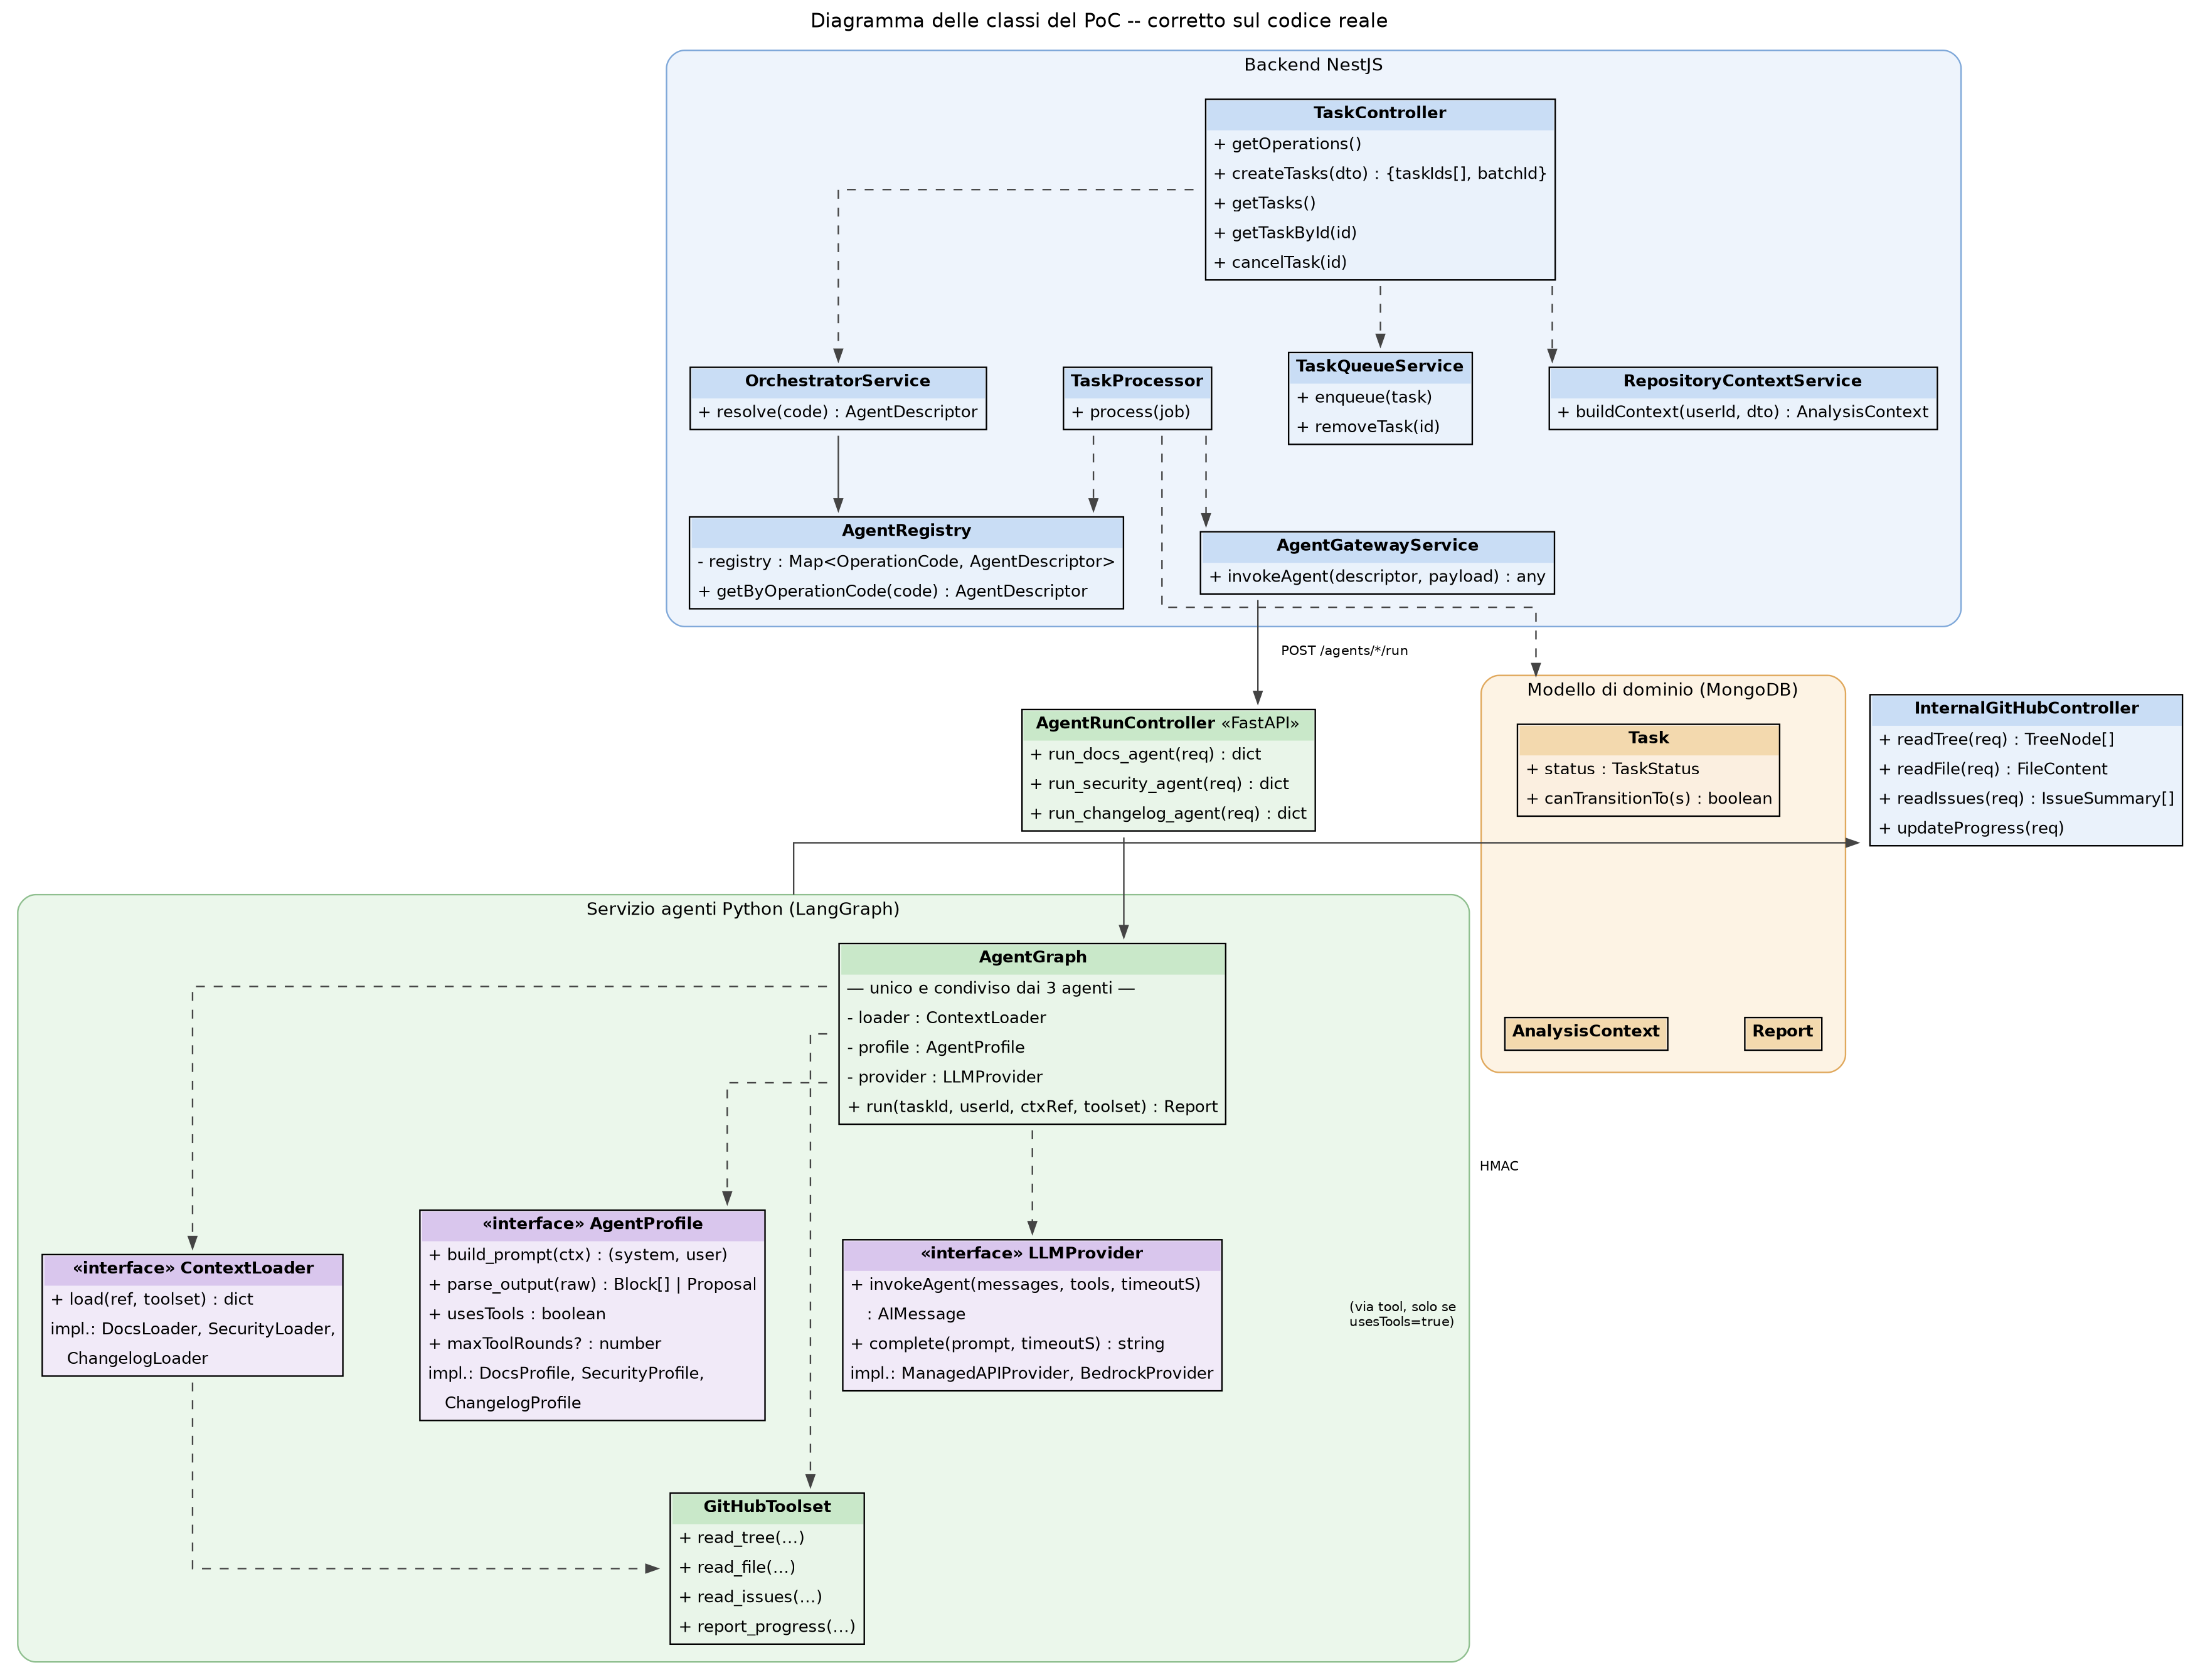
\includegraphics[width=\textwidth]{figures/class_diagram.png}
\caption[Diagramma delle classi]{Diagramma delle classi del PoC.}
\label{fig:class-diagram}
\end{figure}

\begin{figure}[H]
\centering
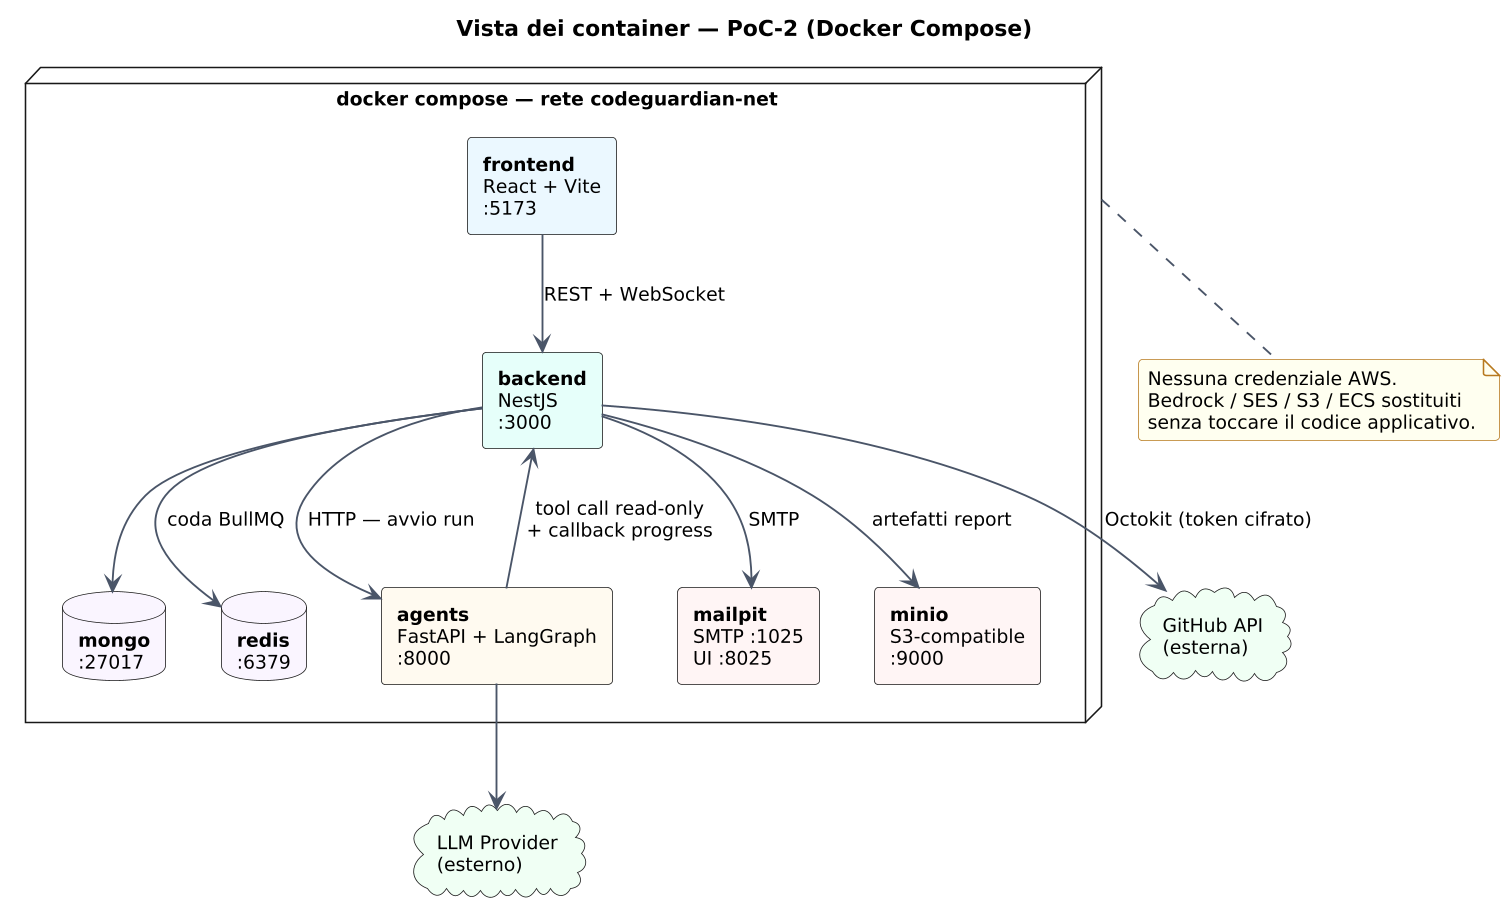
\includegraphics[width=0.95\textwidth]{figures/arch-container.png}
\caption[Architettura a container del PoC]{Architettura a container. Tre servizi portano codice nostro (frontend, backend, agents); i restanti sono infrastruttura. Le uniche connessioni verso l'esterno sono backend$\to$GitHub e agents$\to$provider LLM. La freccia agents$\to$backend (traffico inverso) è la facade di lettura descritta in \S~\ref{sec:github}.}
\label{fig:architettura}
\end{figure}

\subsection{Un solo scheletro, tre configurazioni}
\label{sec:scheletro-condiviso}
L'osservazione che rende economico coprire tutti e tre gli agenti resta valida: i tre agenti condividono la stessa struttura interna. Il grafo LangGraph è fisso, ed è più articolato di un semplice ``carica contesto $\to$ costruisci prompt $\to$ chiama il modello'': oltre ai nodi di caricamento contesto, composizione del prompt, invocazione del modello, validazione/parsing e assemblaggio del report, il grafo include un nodo di \textbf{esecuzione dei tool} con un arco condizionale che, quando il modello richiede una chiamata, riporta l'esecuzione al nodo di invocazione del modello: è il loop che permette a un agente di leggere un file, ricevere il contenuto, e decidere se leggerne un altro prima di rispondere. Questo loop è predisposto nello scheletro condiviso ma viene effettivamente percorso solo dagli agenti che lo attivano. Ciò che varia da un agente all'altro resta comunque confinato in due porte (nel senso di \emph{ports-and-adapters}). Lungo il grafo scorre un unico oggetto di stato, \texttt{AgentState}, che i nodi leggono e arricchiscono: parte da \{\texttt{context\_ref}, \texttt{profilo}\}, si popola con il contesto caricato, il prompt, la cronologia dei messaggi scambiati col modello (comprese le eventuali chiamate a tool e i loro risultati), la risposta grezza, i blocchi o la proposta, e infine il report; un campo \texttt{error} opzionale devia verso lo stato fallito.

Le porte che variano sono due:
\begin{itemize}
  \item \textbf{ContextLoader} --- dato un riferimento, restituisce il contesto iniziale da dare al modello. Nel PoC-2 gli adattatori \textbf{non} leggono più da clone locale o fixture: leggono dal repository reale attraverso i tool della facade GitHub. Per Docs e Changelog questo passo carica \emph{tutto} ciò che serve (rispettivamente: albero e contenuto dei file dell'ambito per Docs; le issue chiuse per Changelog), perché questi due agenti non hanno tool a disposizione durante l'esecuzione del grafo e devono ricevere l'intero materiale già pronto nel prompt. Per Security, invece, \texttt{ContextLoader} carica solo l'albero del repository (e l'eventuale \texttt{POLICY.md}): il contenuto dei singoli file non viene letto in questo passo, ma più avanti nel grafo, durante il ciclo di invocazione del modello, tramite i tool descritti sotto.
  \item \textbf{AgentProfile} --- incapsula le cose specifiche di ogni agente: costruire il prompt (caricando il template esterno e iniettando il contesto: è qui che vive l'isolamento dei prompt) e rileggere la risposta (validarla e trasformarla nei blocchi del report secondo lo schema dell'agente). Il profilo dichiara inoltre se l'agente ha accesso ai tool di lettura durante l'esecuzione (\texttt{usesTools}) e, in caso affermativo, quante iterazioni del ciclo modello$\to$tool$\to$modello sono ammesse prima di considerare l'agente fallito (\texttt{maxToolRounds}). È questo flag, letto dallo scheletro condiviso, a decidere se il grafo percorre il nodo di esecuzione tool oppure lo salta: per Docs e Changelog è disattivato, per Security è attivo con un tetto di iterazioni.
\end{itemize}

C'è poi una terza porta, \texttt{LLMProvider}, condivisa e identica per tutti: cambia solo per configurazione, non per agente. È questa astrazione a rendere il passaggio a Bedrock un cambio di configurazione. Il metodo principale non è una singola chiamata testo-a-testo, ma un'invocazione che riceve anche l'elenco dei tool disponibili (eventualmente vuoto) e la cronologia dei messaggi, così da poter restituire sia una risposta finale sia una richiesta di chiamata a un tool.

Rispetto alla prima stesura, il core dell'agente non è più invocato da un driver a riga di comando, ma da un use case del backend NestJS, che inietta \texttt{context\_ref} e \texttt{profilo}, avvia il grafo ed espone il \texttt{Report} risultante come risposta REST.

\begin{lstlisting}[caption={Porte dell'agente e composizione degli adapter. ContextLoader e AgentProfile variano per agente; il ciclo di tool-calling è parte dello scheletro condiviso ma è attivo solo per i profili con usesTools=true.}]
// Porte (interfacce) -- l'unico codice che varia per agente
interface ContextLoader { load(ref): LoadedContext }   // via facade GitHub
interface AgentProfile  { build_prompt(ctx): Prompt
                          parse_output(raw): Block[] | Proposal
                          usesTools: boolean            // false per Docs, Changelog
                          maxToolRounds?: number }       // usato solo se usesTools = true

interface LLMProvider   {                               // condiviso
  invokeAgent(messages: Message[], tools: Tool[], timeoutS): AIMessage
  complete(prompt: string, timeoutS): string             // scorciatoia quando tools = []
}

// Composizione degli adapter per agente (3 Loader, 7 Profile -- uno per OperationCode)
Docs/README   -> GitHubCodeLoader   + DocsReadmeProfile        (usesTools: false)
Docs/Inline   -> GitHubCodeLoader   + DocsInlineProfile        (usesTools: false)
Docs/API      -> GitHubCodeLoader   + DocsApiProfile           (usesTools: false)
Security/OWASP  -> GitHubTreeLoader + OwaspScanProfile         (usesTools: true, maxToolRounds: 8)
Security/Policy -> GitHubTreeLoader + SecurityPolicyProfile    (usesTools: true, maxToolRounds: 8)
                                      (legge anche POLICY.md)
Changelog/Tech  -> GitHubIssuesLoader + ChangelogTechnicalProfile (usesTools: false)
Changelog/Biz   -> GitHubIssuesLoader + ChangelogBusinessProfile  (usesTools: false)

% Backend NestJS -- sostituisce il driver CLI
POST /contexts { repoOwner, repoName, ref, scopeType, paths? } -> 201 { contextId }
GET  /operations -> elenco OperationDescriptorDto disponibili per l'UI
POST /tasks { contextId, operations: OperationCode[] } -> 202 { taskIds: string[], batchId }
GET  /tasks?{query} -> TaskSummaryDto[]
GET  /tasks/:id -> TaskDetailDto
POST /tasks/:id/cancel -> void
GET  /reports/:id -> Report persistito su MongoDB
GET  /reports/:id/export?format=md -> file scaricabile (Report -> Markdown)
WS   task.progress / task.updated -> avanzamento e stato finale (non polling)
\end{lstlisting}

Il frontend costruisce prima l'\texttt{AnalysisContext} tramite
\texttt{POST /contexts} (repository, ambito, riferimento), quindi avvia
una o più operazioni con \texttt{POST /tasks}, che risponde immediatamente
con gli identificativi delle task create in stato \texttt{PENDING} e non
con il report. L'avanzamento e la transizione di stato (\texttt{COMPLETED},
\texttt{FAILED}, \texttt{CANCELLED}) arrivano via WebSocket
(\texttt{task.progress}, \texttt{task.updated}), non tramite interrogazione
ripetuta di \texttt{GET /reports/:id}. Gli endpoint \texttt{/internal/*}
restano riservati alla comunicazione agente\textrightarrow{}backend e non
sono mai chiamati dal frontend.

\subsection{Modello di dominio}
\label{sec:domain-model}
Il diagramma in figura~\ref{fig:domain-model} mostra le entità persistite su MongoDB. Al centro c'è \texttt{Task}: ogni esecuzione richiesta
dall'utente ne è un'istanza. Attorno ruotano \texttt{AnalysisContext} (su cosa si lavora:
repository, riferimento risolto a SHA, ambito), \texttt{OperationCode} (cosa si fa: la chiave
che l'orchestratore usa per instradare) e \texttt{Report} (cosa ne è uscito). L'\texttt{AccessLog}
registra ogni lettura effettuata su GitHub per conto di una task -- nello schema reale i campi
sono \texttt{taskId}, \texttt{endpoint} e \texttt{resource} (non esistono un \texttt{userId} né
un campo \texttt{operation} propri del log: l'endpoint richiamato già identifica il tipo di
lettura) -- ed è l'evidenza che rende verificabile il vincolo di sola lettura.

\texttt{AnalysisContext} è deliberatamente persistito e non passato inline: più task dello
stesso avvio lo condividono senza duplicarlo, e il pin del riferimento a uno SHA rende i
report riproducibili anche dopo nuovi commit sul repository. Il campo opzionale
\texttt{sprintId} è usato solo dall'operazione Changelog, per filtrare le issue sulla
milestone richiesta.\texttt{AnalysisContext} non espone alcun metodo di validazione dimensionale:
il controllo sulla dimensione del contesto (\texttt{max\_scope\_chars}, fissato a \textbf{60.000 caratteri}, equivalenti a circa 15.000 token per i modelli Qwen3) è implementato lato
agente Python, nel nodo \emph{componi\_prompt} del grafo LangGraph.

Il \texttt{Report} è un envelope unico e generico: qualunque sia l'agente che lo produce, la
struttura è sempre \texttt{\{..., body: Block[], proposal?: Proposal, error?: ReportError\}}.

Infine, \texttt{ServiceCredential} custodisce il token GitHub cifrato: oltre a
\texttt{ciphertext} e \texttt{authTag}, lo schema reale include \texttt{iv} (vettore di
inizializzazione) e \texttt{salt}, entrambi necessari alla cifratura AES; il campo \texttt{provider} è una stringa libera
(di fatto sempre \texttt{"GITHUB"} in questo PoC), non un'enumerazione chiusa. Gli
sviluppatori implementano questi schemi con Mongoose.

\begin{figure}[h]
  \centering
  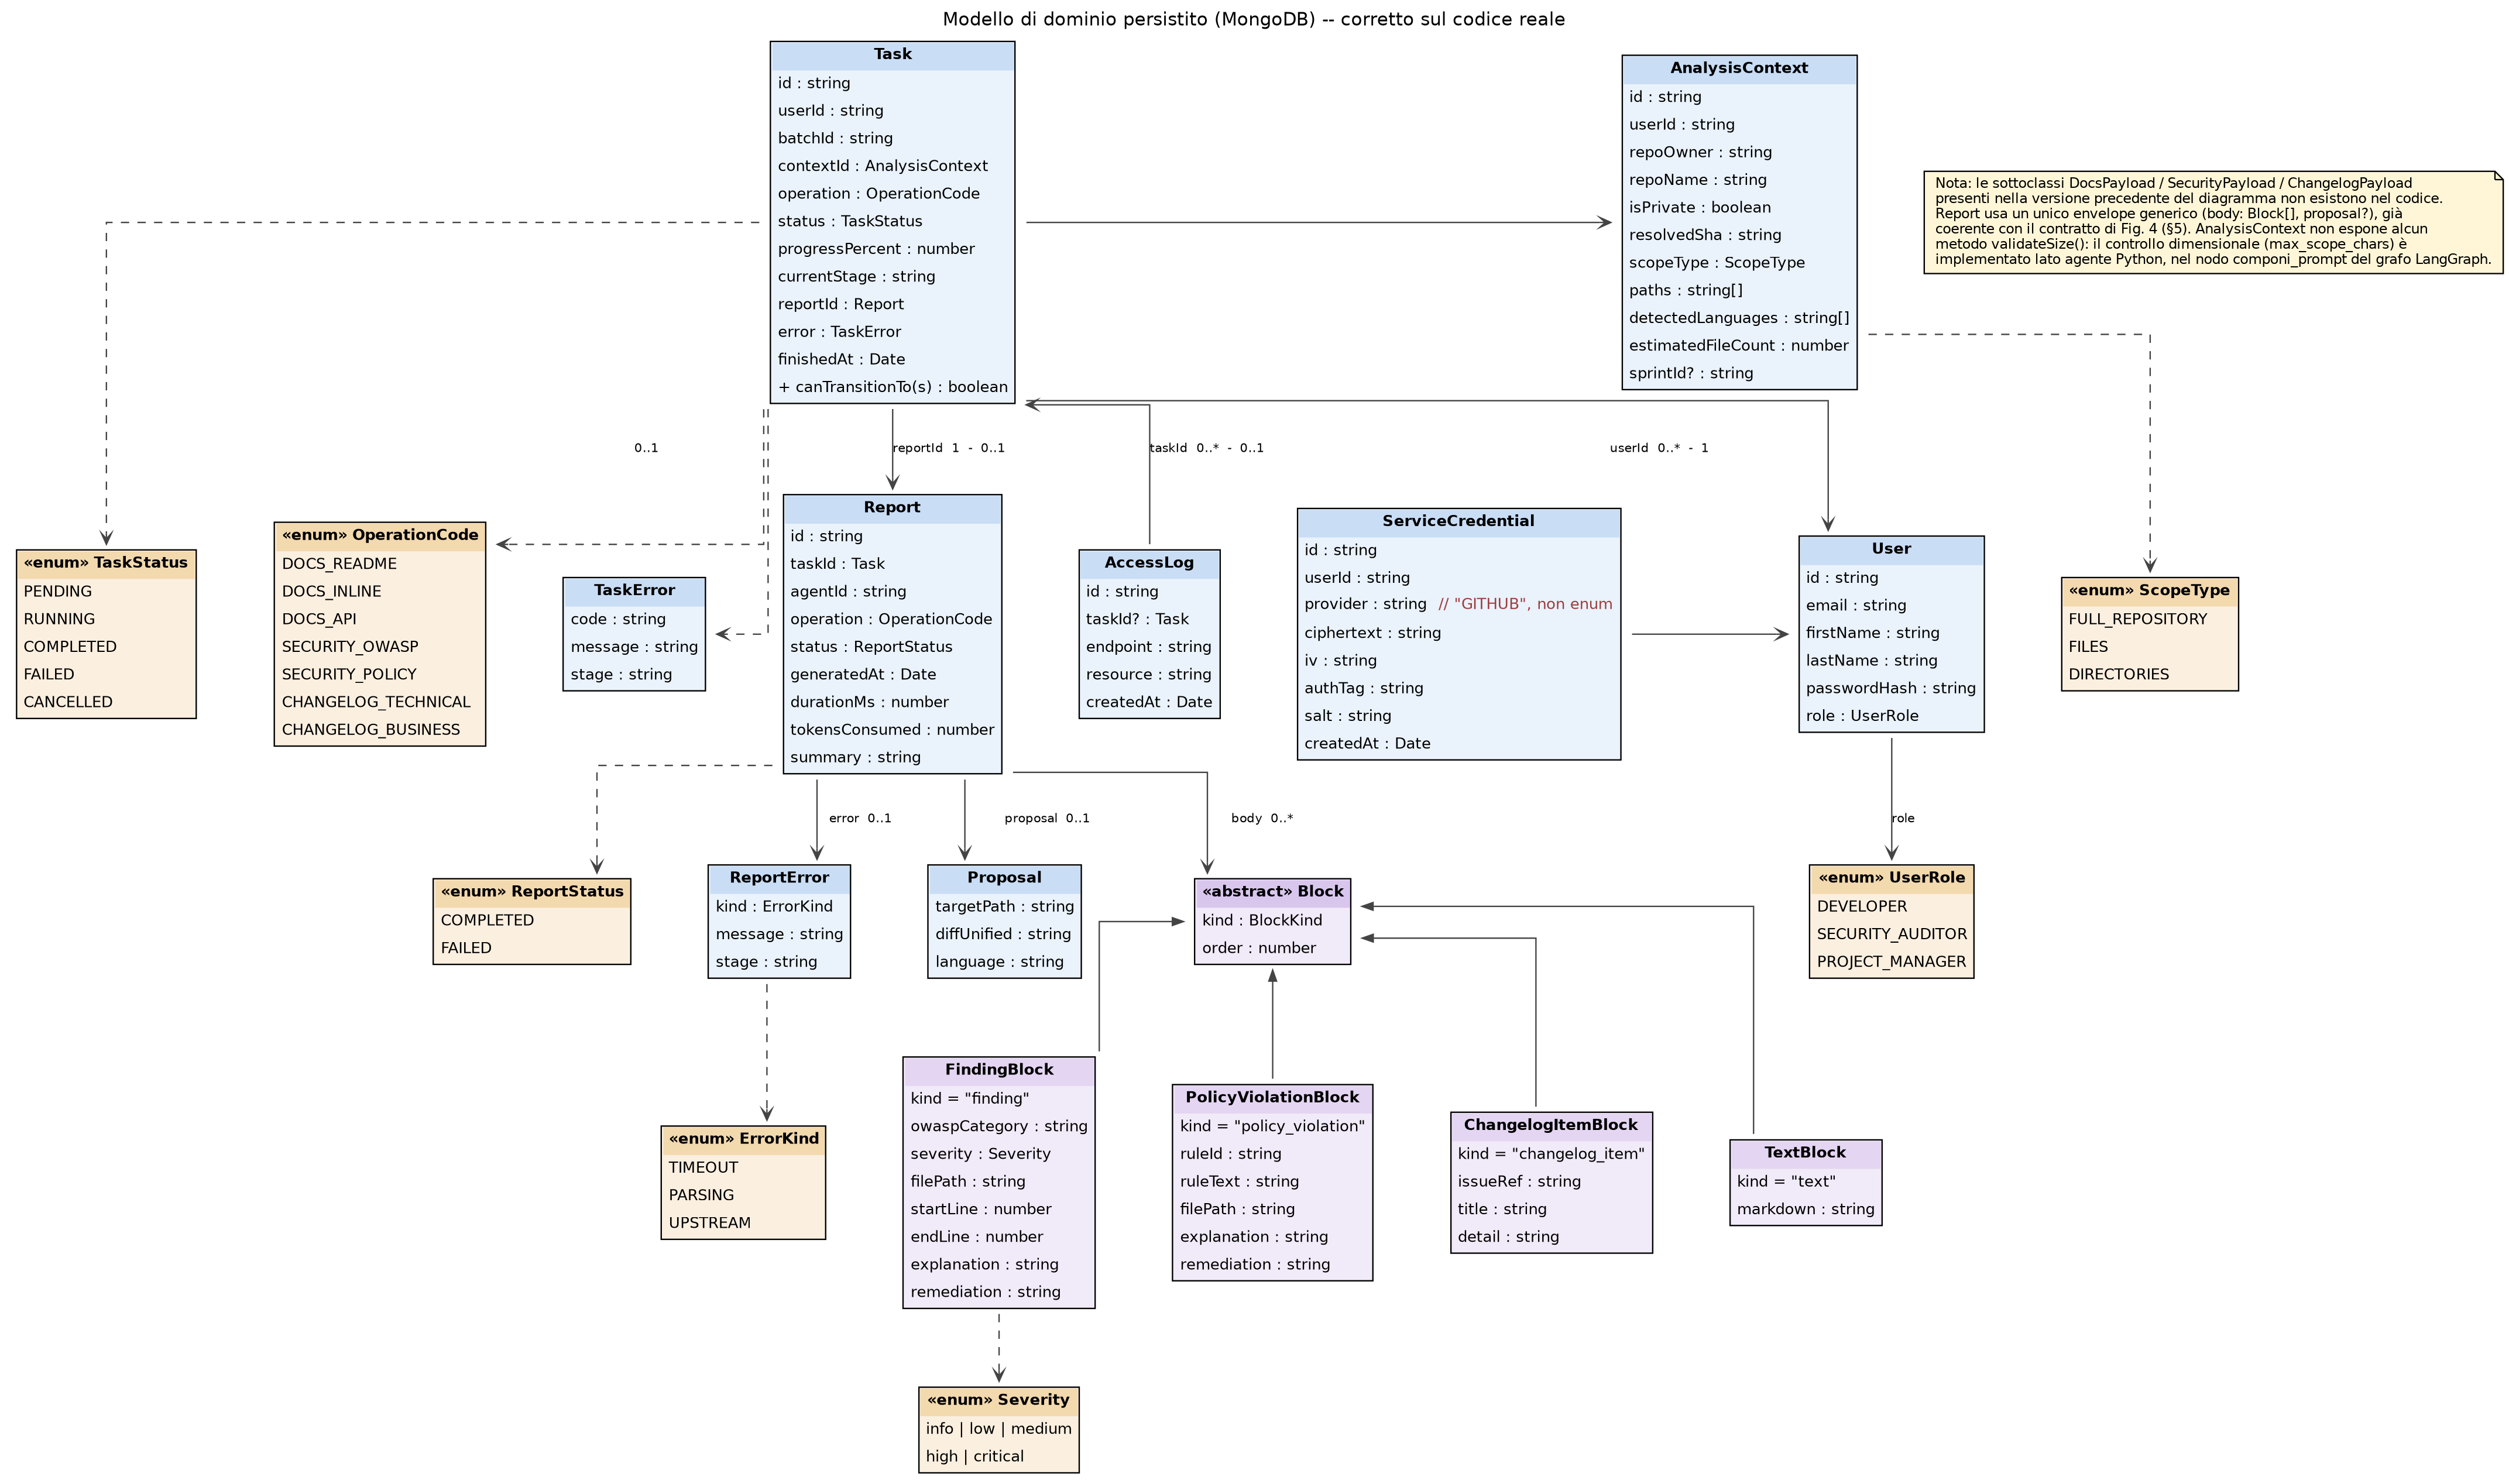
\includegraphics[width=\textwidth]{figures/fig3_domain_model_corretta.png}
  \caption{Modello di dominio persistito su MongoDB, corretto sul codice reale. Le
  sottoclassi \texttt{Payload} sono state rimosse (ridondanti con la figura~\ref{fig:report});
  \texttt{AccessLog} e \texttt{ServiceCredential} riportano i campi effettivamente presenti
  negli schemi Mongoose.}
  \label{fig:domain-model}
\end{figure}

\section{Il contratto di output condiviso}
\label{sec:contratto}

Il nodo finale del grafo, \emph{Assembla report}, produce sempre lo stesso oggetto \texttt{Report}, qualunque sia l'agente. È questo a rendere i tre output un contratto unico: sia il backend sia il frontend trattano sempre un \texttt{Report}, senza sapere quale agente l'ha prodotto. La struttura è un \emph{envelope}: un'intestazione comune, un corpo fatto di blocchi ordinati, e un eventuale artefatto di proposta (il diff). Il \texttt{Report} viene persistito su MongoDB dal backend e reso via API REST al frontend, che lo renderizza nell'interfaccia grafica.

\begin{figure}[H]
\centering
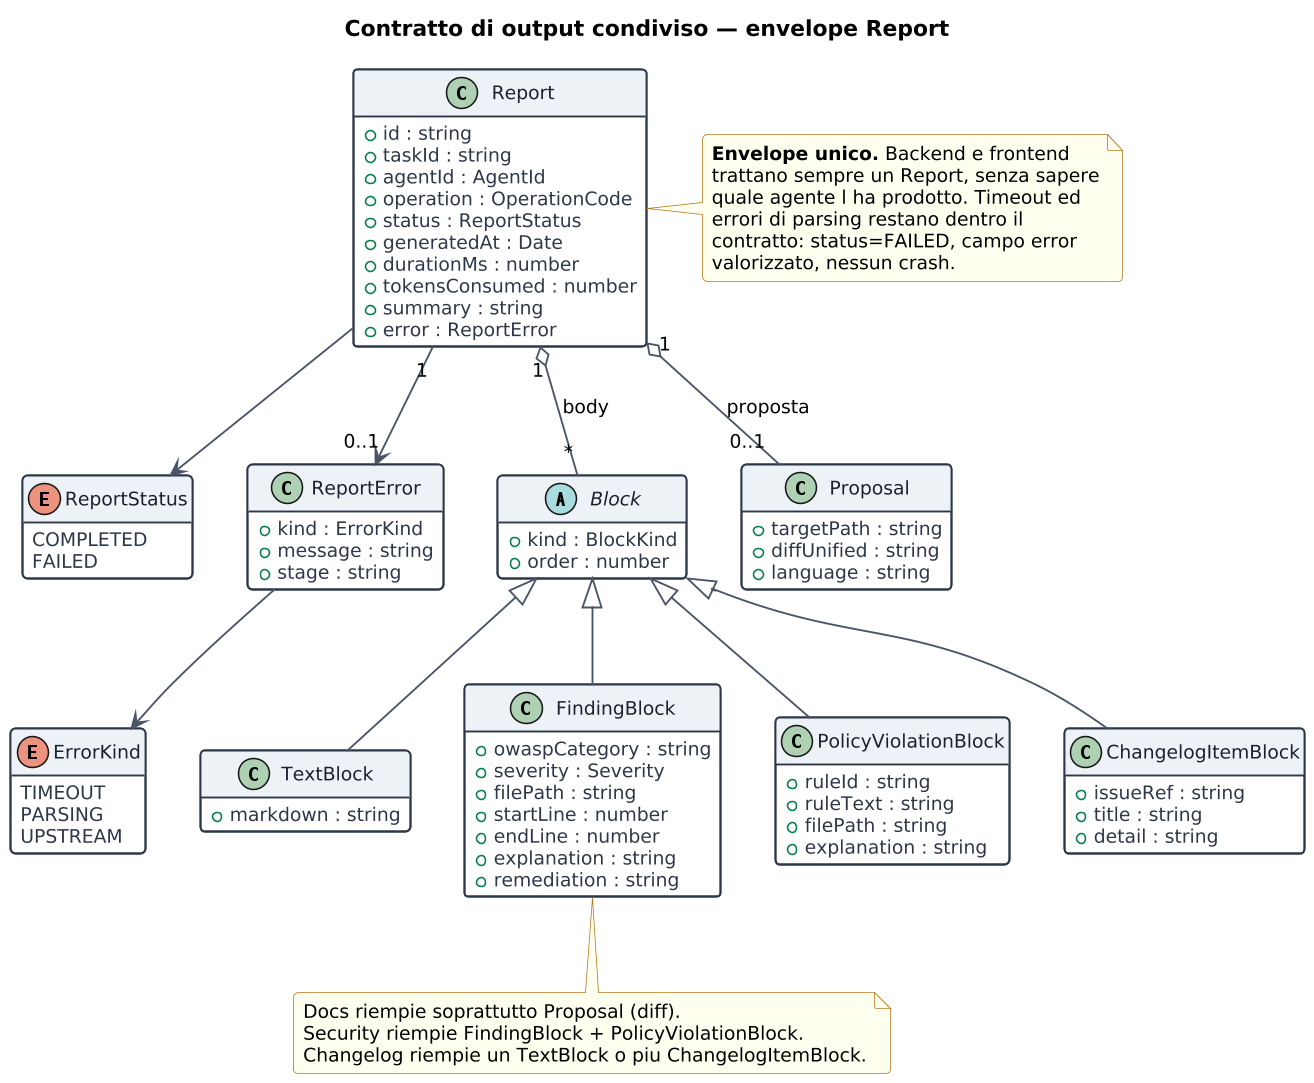
\includegraphics[width=0.82\textwidth]{figures/report-contract.png}
\caption[Contratto Report]{Il contratto \texttt{Report}: envelope comune, blocchi polimorfi nel corpo, proposta opzionale. Timeout ed errori di parsing restano dentro il contratto (\texttt{status=FAILED}, campo \texttt{error} valorizzato), senza provocare crash.}
\label{fig:report}
\end{figure}

Ogni agente riempie lo stesso envelope in modo diverso: Security con \texttt{FindingBlock} ed eventuale \texttt{PolicyViolationBlock}; Docs soprattutto con una \texttt{Proposal} di diff; Changelog con un \texttt{TextBlock} o più \texttt{ChangelogItemBlock}. In tutti i casi, timeout ed errori di parsing non provocano crash: valorizzano \texttt{error} e portano \texttt{status} a \texttt{FAILED}, restando dentro il contratto; il frontend mostra questi stati con un componente di errore dedicato, senza gestione speciale lato backend.

\section{Integrazione con GitHub}
\label{sec:github}

Questa è la sezione che gli sviluppatori devono leggere con più attenzione, perché è dove è più facile sbagliare in un modo che viola un vincolo di sicurezza. La regola da tenere ferma è una sola: \textbf{il token GitHub non lascia mai il backend NestJS}, e \textbf{gli agenti non chiamano mai GitHub direttamente}.

\subsection{Come l'agente legge dal repository}

L'agente non possiede il token e non conosce l'URL di GitHub. Quando ha bisogno di leggere qualcosa, invoca un \emph{tool} LangGraph che, sotto il cofano, chiama un endpoint interno del backend. È il backend a decifrare il token, chiamare GitHub in sola lettura, registrare l'accesso e restituire il contenuto. La figura~\ref{fig:github} mostra le classi coinvolte.

\begin{figure}[H]
\centering
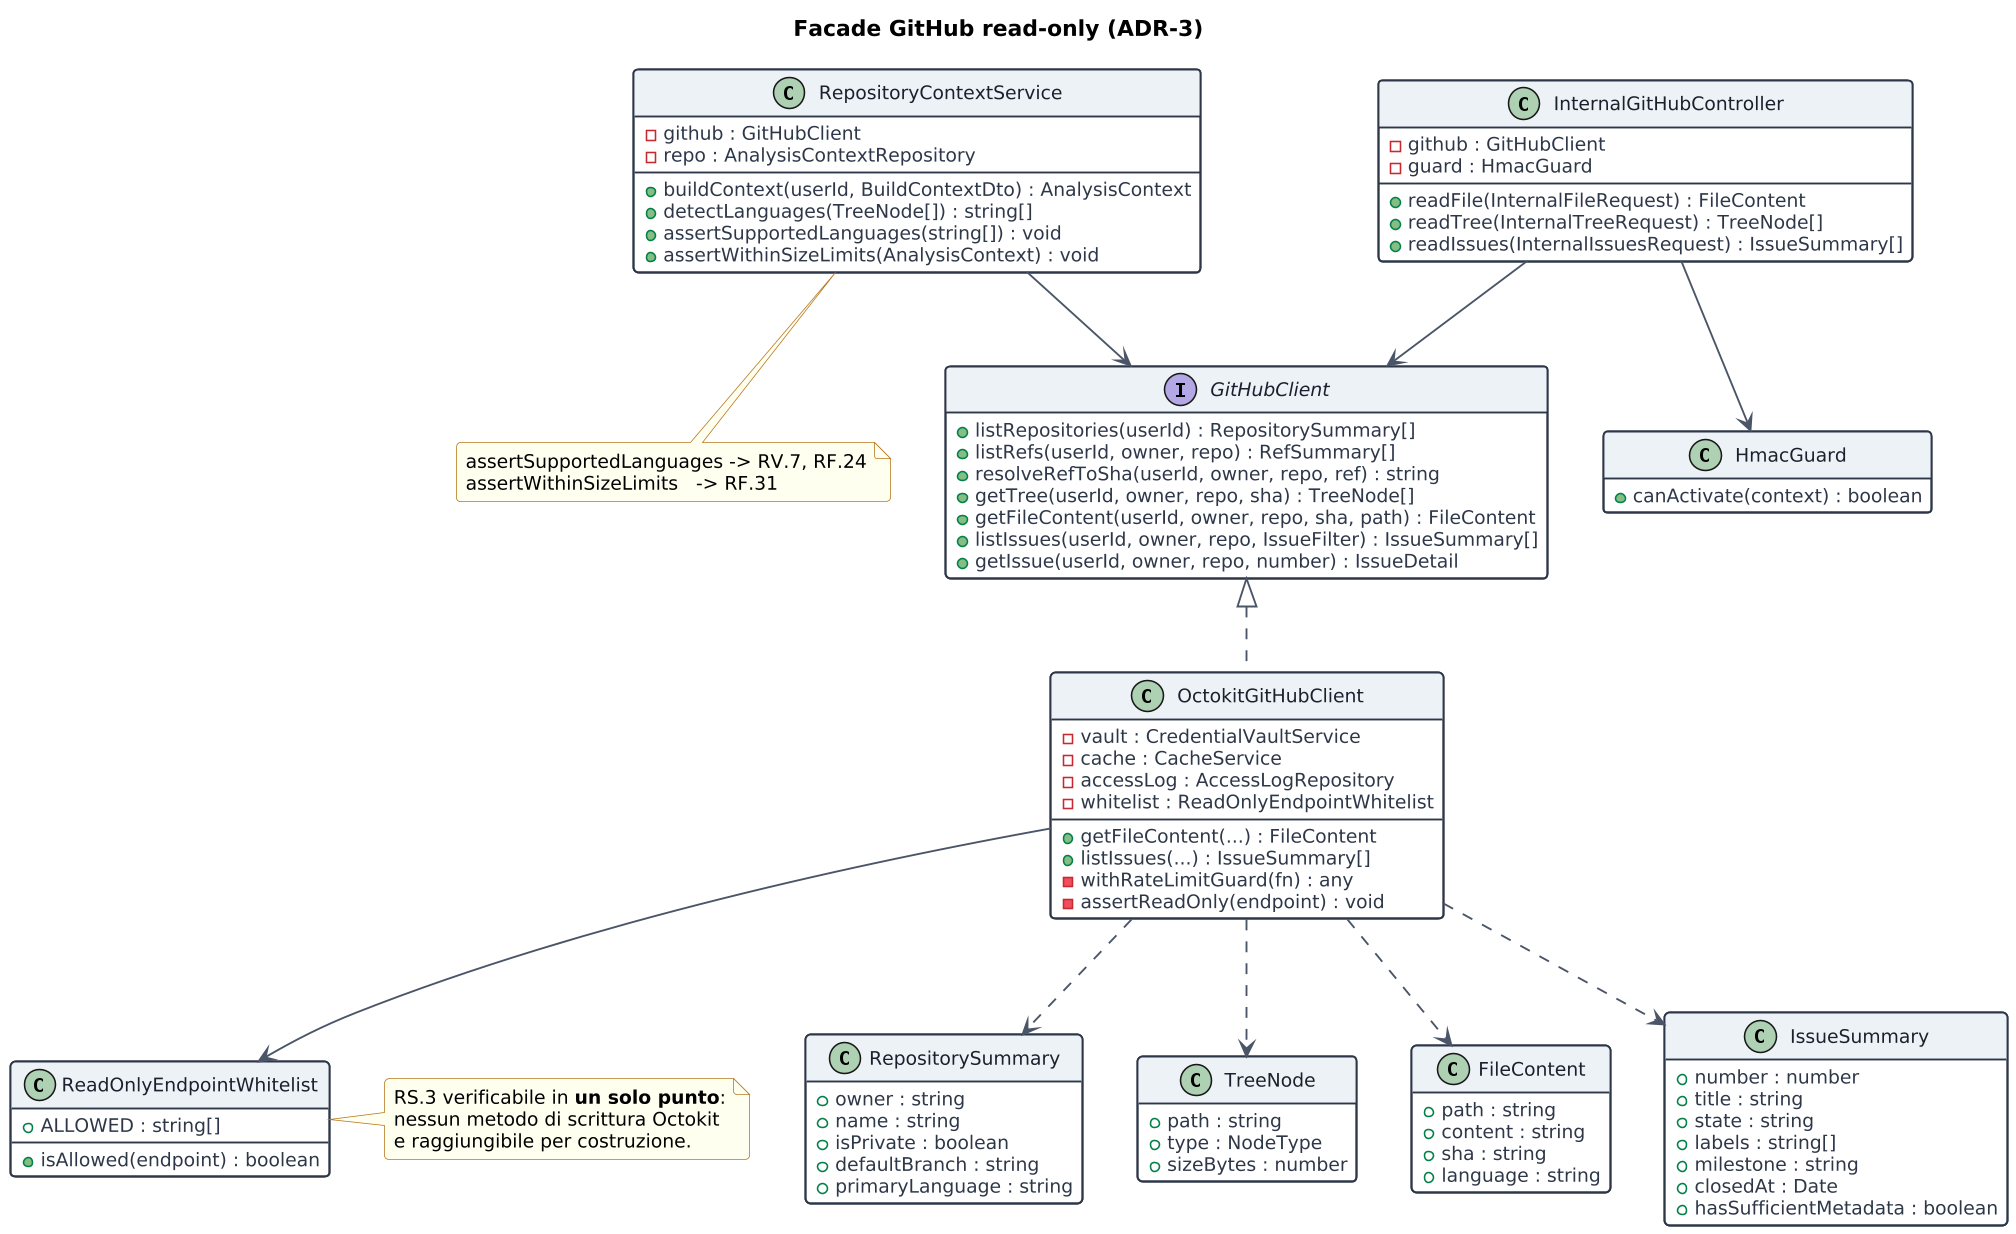
\includegraphics[width=0.95\textwidth]{figures/github-facade.png}
\caption[Facade GitHub read-only]{La facade GitHub. \texttt{ReadOnlyEndpointWhitelist} rende il vincolo di sola lettura verificabile in un solo punto: nessun metodo di scrittura è raggiungibile per costruzione. Gli endpoint \texttt{/internal/*} sono usati dagli agenti e protetti da HMAC.}
\label{fig:github}
\end{figure}

I tool disponibili all'agente sono tre, tutti di lettura: \texttt{read\_tree} (struttura del repository a un dato SHA), \texttt{read\_file} (contenuto di un file) e \texttt{read\_issues} (elenco e dettaglio delle issue, filtrabili). Mentre l'agente Security sfrutta un vero tool-calling autonomo e iterativo per esplorare i file, gli agenti Docs e Changelog seguono un flusso deterministico: un loader Python pre-carica interamente il contesto (file di codice o issue) prima dell'invocazione del modello, al quale viene esplicitamente vietato l'uso di tool esterni, ed è ciò che le stesure precedenti non dimostravano.

\subsection{I quattro controlli su ogni chiamata}

Ogni lettura verso GitHub attraversa quattro meccanismi, che gli sviluppatori implementano una sola volta in \texttt{OctokitGitHubClient}:

\begin{itemize}
  \item \textbf{Whitelist} (\texttt{ReadOnlyEndpointWhitelist}): se un endpoint non è nell'elenco chiuso di operazioni di lettura, la chiamata non parte. Il vincolo RS.3 non dipende dall'attenzione di chi scrive il codice, ma è garantito per costruzione.
  \item \textbf{Cache Redis} con chiave \texttt{repo@sha:path}: poiché il contesto è pinnato a uno SHA, il contenuto di un file a quel commit è immutabile e la cache non può servire dati stantii. Serve a contenere il consumo di rate limit quando l'agente rilegge lo stesso file in iterazioni diverse.
  \item \textbf{Rate limit guard}: legge le intestazioni di quota di GitHub e, in prossimità dell'esaurimento, rallenta invece di fallire.
  \item \textbf{AccessLog}: ogni chiamata lascia una riga con task, endpoint e risorsa. È l'evidenza che rende RS.3 dimostrabile invece che dichiarata.
\end{itemize}

\subsection{Autenticazione degli endpoint interni}

Gli endpoint \texttt{/internal/github/*} e \texttt{/internal/tasks/:id/progress} non sono esposti al frontend e non compaiono nello Swagger pubblico. Sono raggiungibili solo dalla rete Docker e autenticati con \textbf{HMAC-SHA256} tramite un segreto condiviso tra backend e servizio agenti (\texttt{INTERNAL\_SHARED\_SECRET}), perché il chiamante non è un utente ma un servizio. Gli sviluppatori del servizio agenti firmano ogni richiesta; gli sviluppatori del backend verificano la firma in un guard dedicato (\texttt{InternalAuthGuard}).

Il messaggio firmato ha la struttura:
\begin{center}
\texttt{HMAC-SHA256(timestamp + ":" + method + ":" + path + ":" + bodyHash,\ INTERNAL\_SHARED\_SECRET)}
\end{center}
dove \texttt{timestamp} è lo Unix timestamp in secondi (stringa), \texttt{method} è il verbo HTTP in maiuscolo (\texttt{POST}, \texttt{GET}), \texttt{path} è il path completo senza query string (es.\ \texttt{/internal/tasks/abc123/progress}) e \texttt{bodyHash} è lo SHA-256 hex del body JSON (stringa vuota \texttt{""} per request senza body). La finestra anti-replay è di $\pm\texttt{HMAC\_WINDOW\_S}$ secondi (default 30). La request include gli header:
\begin{center}
\texttt{X-Internal-Timestamp: <timestamp>} \quad \texttt{X-Internal-Signature: <hmac-hex>}
\end{center}

\subsection{Il caso dell'Agente Docs}

L'Agente Docs merita una nota, perché è l'unico che \emph{produce un file che potrebbe già esistere} nel repository, e quindi il vincolo di sola lettura sembra confliggere con la sua funzione. Non è così: l'agente legge dal repository ma non ci scrive.

\begin{figure}[H]
\centering
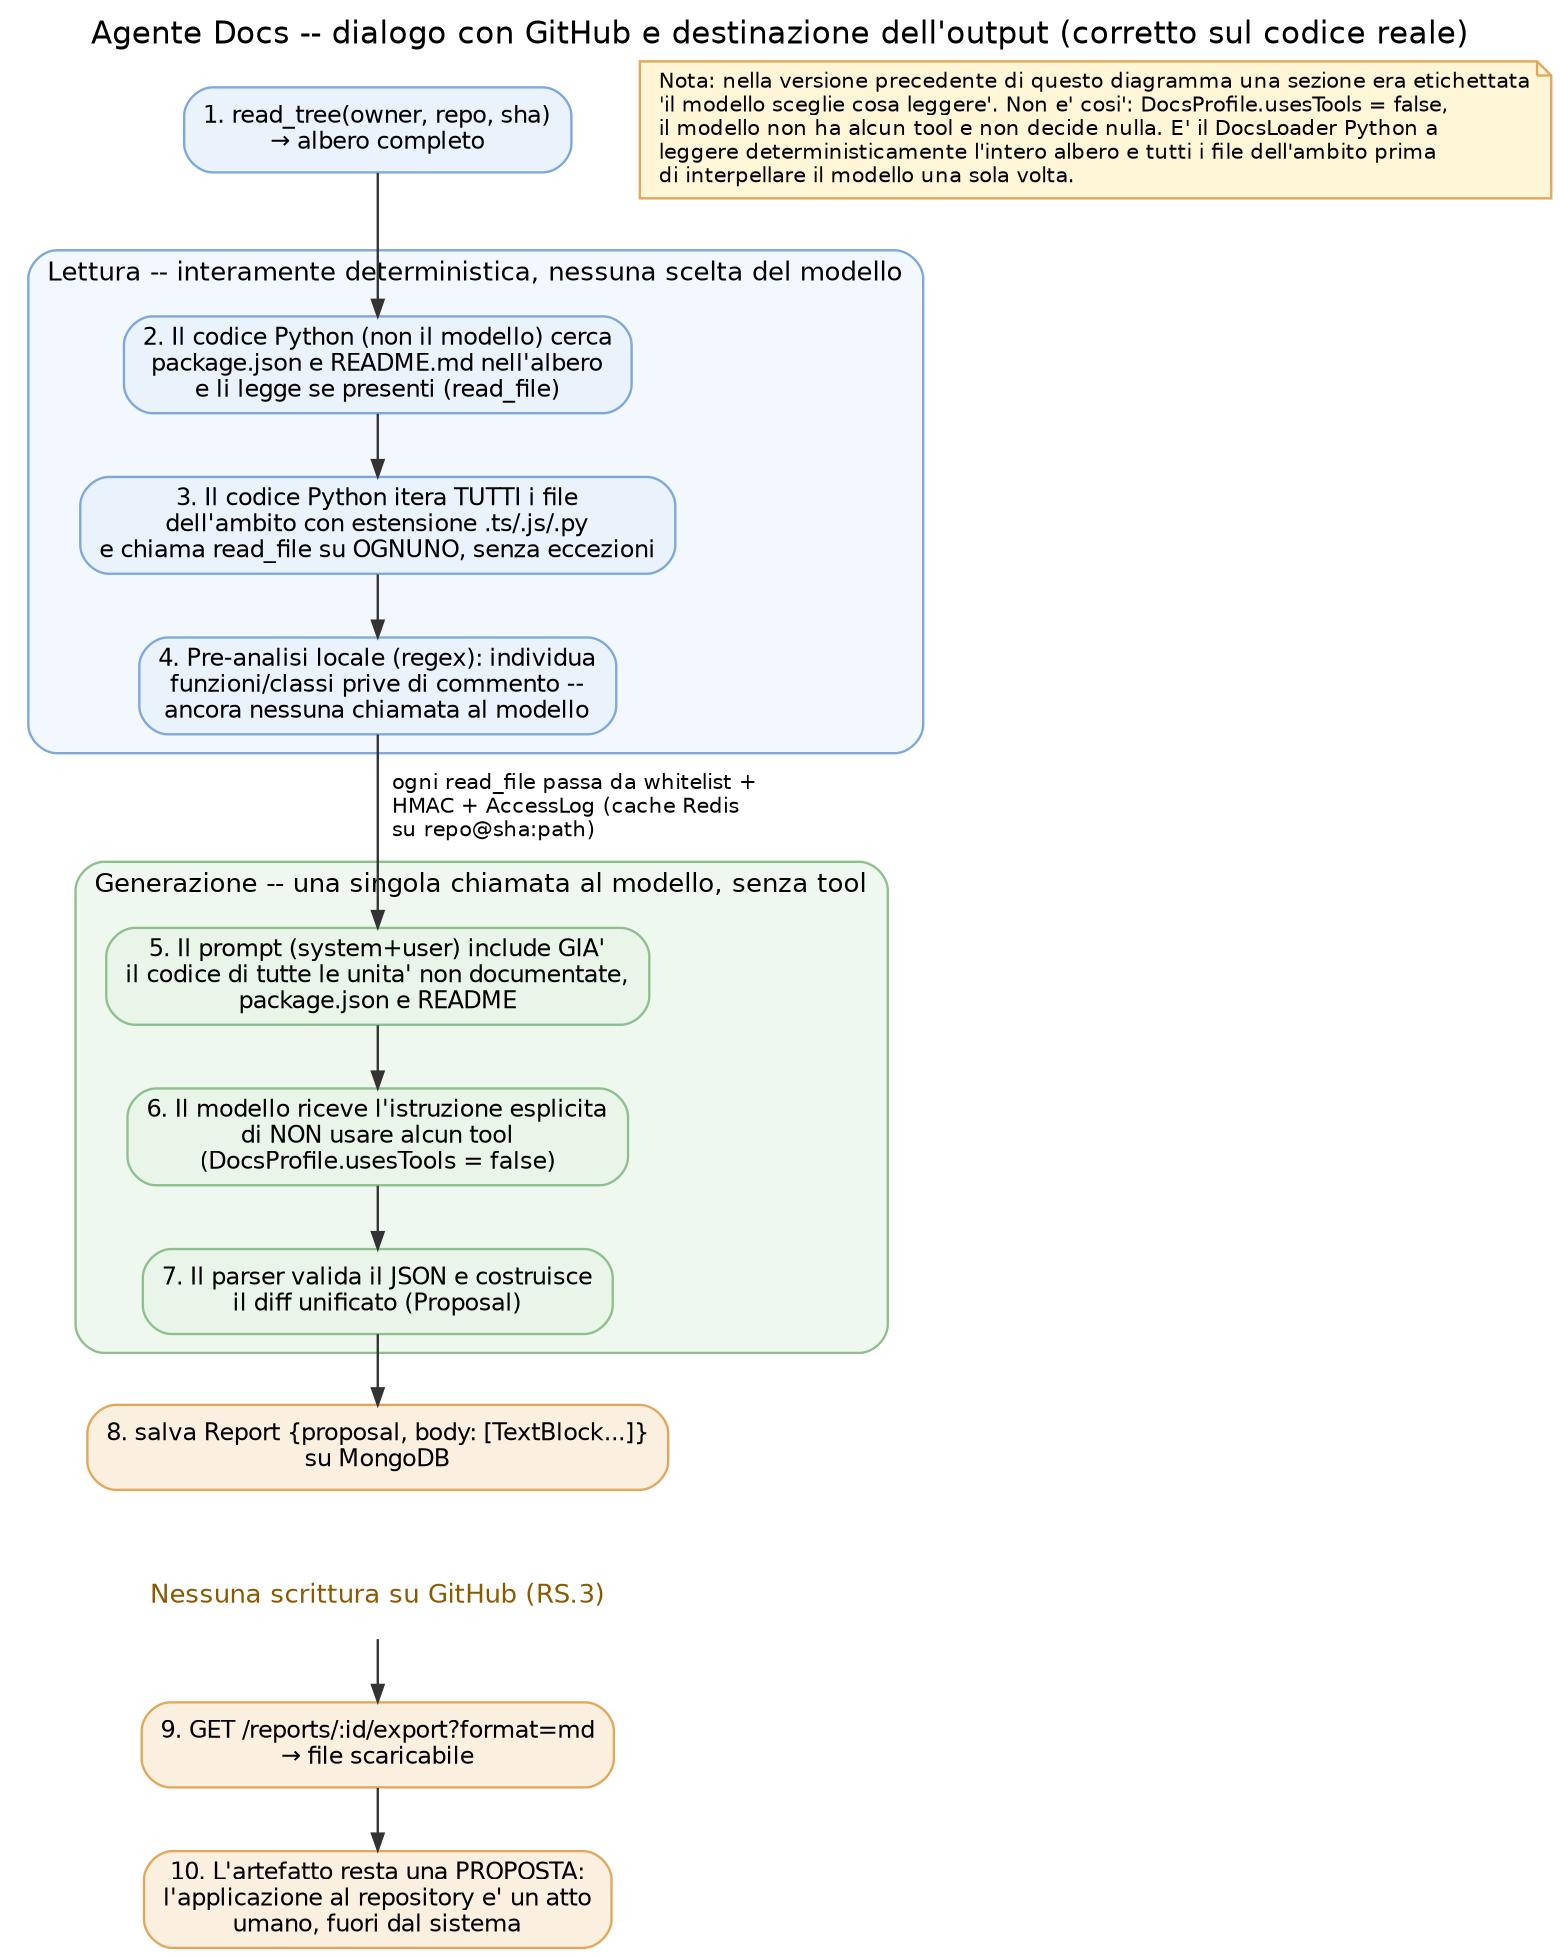
\includegraphics[width=0.80\textwidth]{figures/docs.png}
\caption[Agente Docs e destinazione dell'output]{Agente Docs: legge in modo più esteso degli altri (deve prima capire che progetto è), ma in scrittura produce solo una proposta di diff salvata come \texttt{Report}. Nel PoC l'applicazione al repository è un atto umano (nessuna PR viene aperta). \textbf{Aggiornamento MVP}: il backend apre la Pull Request automaticamente ricevuta la \texttt{Proposal} (ADR-AWS-10, \S~\ref{sec:aws-adr}); il \emph{merge} resta un atto umano condotto su GitHub.}
\label{fig:docs}
\end{figure}

In lettura, l'Agente Docs ha un profilo diverso dagli altri: mentre Security legge pochi file mirati in profondità, Docs deve prima capire \emph{che progetto è}, quindi parte con un'esplorazione a largo raggio (albero completo, \texttt{package.json}, README esistente). La presenza di un README trasforma il compito da generazione ad aggiornamento. In scrittura, l'output è un \texttt{Proposal} (diff verso il file di destinazione) salvato come \texttt{Report}: l'applicazione al repository resta un atto umano, coerente con RS.3.

\section{Contratto delle API: comunicazione frontend--backend}
\label{sec:api}

Questa sezione è il riferimento operativo per chi implementa il backend (deve realizzare questi endpoint) e per il progettista frontend (deve sapere quali chiamare da ogni pagina). Elenca il contratto in modo che le due parti possano procedere in parallelo senza ambiguità.

\subsection{Due piani di comunicazione distinti}

Il punto da cui partire, perché è la fonte di errore più comune: esistono \textbf{due piani di comunicazione separati}, e il frontend ne usa uno solo.

Il frontend è un'applicazione React che gira \textbf{nel browser dell'utente}, non dentro la rete Docker. Raggiunge quindi il backend attraverso la porta esposta sull'host (\texttt{localhost:3000}), non attraverso l'hostname interno del container. Gli agenti Python, invece, vivono \emph{dentro} la rete Docker e raggiungono il backend all'hostname interno (\texttt{backend:3000}) su endpoint diversi, protetti da HMAC (\S~\ref{sec:github}). Il frontend non tocca mai gli endpoint interni, e gli agenti non toccano mai quelli pubblici: è questa separazione a garantire che il token GitHub non lasci il backend (ADR-1).

\begin{table}[H]
\centering
\caption{Indirizzi base dei servizi in ambiente di sviluppo.}
\label{tab:indirizzi}
\vspace{2mm}
\renewcommand{\arraystretch}{1.2}
\begin{tabularx}{\textwidth}{|l|l|l|}
\hline
\textbf{Servizio} & \textbf{Dal browser} & \textbf{Nella rete Docker} \\ \hline
Frontend (Vite) & \texttt{http://localhost:5173} & \texttt{http://frontend:5173} \\ \hline
Backend (NestJS) & \texttt{http://localhost:3000} & \texttt{http://backend:3000} \\ \hline
Agenti (FastAPI) & --- (non esposto) & \texttt{http://agents:8000} \\ \hline
\end{tabularx}
\end{table}

Il frontend non ha l'indirizzo del backend cablato nel codice: lo legge dalla variabile \texttt{VITE\_\allowbreak{}API\_\allowbreak{}BASE\_\allowbreak{}URL}, così in produzione cambia senza ricompilare. Il backend adotta un prefisso globale versionato (\texttt{app.\allowbreak{}setGlobalPrefix('api/v1')}), quindi la base REST effettiva è \texttt{http://\allowbreak{}localhost:3000/\allowbreak{}api/v1}. Sia il prefisso \texttt{/api/v1} sia la scelta del canale realtime (WebSocket, \S~\ref{sub:ws}) sono proposte del progettista: se il team decide diversamente, questa sezione è il punto in cui aggiornarle.

\subsection{API REST pubbliche (browser $\to$ backend)}

Tutti i path che seguono sono relativi alla base \texttt{/api/v1} e documentati in Swagger, raggiungibile durante lo sviluppo a \texttt{http://localhost:3000/api/docs}. Le chiamate autenticate portano il JWT nell'header \texttt{Authorization: Bearer}.

\begin{table}[H]
\centering
\caption{Endpoint REST pubblici, raggruppati per pagina del frontend.}
\label{tab:rest}
\vspace{2mm}
\renewcommand{\arraystretch}{1.15}
\begin{tabularx}{\textwidth}{|l|X|l|}
\hline
\textbf{Metodo e path} & \textbf{Scopo} & \textbf{Requisiti} \\ \hline
\multicolumn{3}{|l|}{\textit{Autenticazione}} \\ \hline
\texttt{POST /auth/register} & Registrazione di un nuovo utente (stub nel PoC, si veda nota) & RF.1--RF.6 \\ \hline
\texttt{POST /auth/login} & Login, restituisce il JWT (stub nel PoC, si veda nota) & RF.7--RF.9 \\ \hline
\texttt{GET /auth/me} & Profilo dell'utente autenticato & RF.9 \\ \hline
\texttt{GET /auth/health} & Healthcheck del backend (uso interno, Docker Compose) & --- \\ \hline
\multicolumn{3}{|l|}{\textit{Credenziali di servizio}} \\ \hline
\texttt{POST /credentials} & Salva il token GitHub (cifrato) & RF.10--RF.11, RS.2 \\ \hline
\texttt{GET /credentials} & Elenco delle credenziali configurate & RF.12 \\ \hline
\texttt{POST /credentials/:id/validate} & Verifica validità e scope & RF.12, RS.4 \\ \hline
\texttt{DELETE /credentials/:id} & Revoca una credenziale & RF.12 \\ \hline
\multicolumn{3}{|l|}{\textit{Selezione del repository e dell'ambito}} \\ \hline
\texttt{GET /repositories} & Elenco dei repository dell'utente & RF.21--RF.23 \\ \hline
\texttt{GET /repositories/\allowbreak{}:owner/\allowbreak{}:repo/refs} & Branch e tag disponibili & RF.24 \\ \hline
\texttt{GET /repositories/\allowbreak{}:owner/\allowbreak{}:repo/tree?ref=} & Struttura del repository & RF.24--RF.30 \\ \hline
\texttt{POST /contexts} & Crea l'\texttt{AnalysisContext}, ritorna \texttt{contextId} & RF.25--RF.31 \\ \hline
\multicolumn{3}{|l|}{\textit{Avvio ed esecuzione}} \\ \hline
\texttt{GET /operations} & Operazioni disponibili (per i pulsanti) & RF.32--RF.34 \\ \hline
\texttt{POST /tasks} & Avvia una o più task in batch, ritorna 202 + \texttt{\{taskIds[], batchId\}} & RF.35--RF.42 \\ \hline
\texttt{GET /tasks} & Elenco delle task per la dashboard & RF.43--RF.45 \\ \hline
\texttt{GET /tasks/:id} & Dettaglio di una singola task & RF.45 \\ \hline
\texttt{POST /tasks/:id/cancel} & Annulla una task & RF.46 \\ \hline
\multicolumn{3}{|l|}{\textit{Storico e report}} \\ \hline
\texttt{GET /reports?operation=\&from=\&to=} & Storico dei report, filtrabile & RF.49--RF.51 \\ \hline
\texttt{GET /reports/:id} & Dettaglio di un report & UC33 \\ \hline
\texttt{GET /reports/:id/export?format=} & Esporta il report (\texttt{md} o \texttt{json}) & RF.51 \\ \hline
\end{tabularx}
\end{table}

\texttt{POST /auth/register} e \texttt{POST /auth/login} sono implementati come \textbf{stub}: il primo restituisce un messaggio statico senza creare alcun utente, il secondo firma sempre lo stesso JWT per un utente fisso, senza verificare alcuna credenziale. È una scelta coerente con il perimetro dichiarato in \S~\ref{sec:tecnologie} (``il PoC assume un utente già noto''), ma va tenuta presente da chi consuma questo contratto: gli endpoint esistono e rispondono, ma non implementano ancora RF.1--RF.9.

\subsection{Canale realtime (browser $\to$ backend)}
\label{sub:ws}

L'avanzamento delle task arriva al frontend via WebSocket (Socket.IO), coerentemente con l'esecuzione asincrona su coda (ADR-3): la \texttt{POST /tasks} ritorna subito, e il frontend si iscrive al canale usando i \texttt{taskId} ricevuti. La connessione è a \texttt{ws://localhost:3000} e viene autenticata passando il JWT all'handshake. Il server emette quattro eventi verso il client nel PoC; il frontend non emette eventi applicativi, solo iscrizione. \textbf{Nota MVP:} la Parte~\ref{part:backend-mvp} (\S~\ref{sec:be-contratto-api}) aggiunge un quinto evento (\texttt{task.inputRequired}) e costituisce il contratto vincolante per l'implementazione.

\begin{table}[H]
\centering
\caption{Eventi WebSocket emessi dal backend verso il frontend.}
\label{tab:ws}
\vspace{2mm}
\renewcommand{\arraystretch}{1.2}
\begin{tabularx}{\textwidth}{|l|X|X|}
\hline
\textbf{Evento} & \textbf{Payload} & \textbf{Uso nel frontend} \\ \hline
\texttt{task.updated} & \texttt{\{ taskId, status, reportId? \}} & Aggiorna il badge di stato in dashboard \\ \hline
\texttt{task.progress} & \texttt{\{ taskId, stage, percent \}} & Muove la barra di avanzamento \\ \hline
\texttt{task.failed} & \texttt{\{ taskId, error \}} & Mostra un toast; non blocca le altre task \\ \hline
\texttt{batch.completed} & \texttt{\{ batchId, completed, failed \}} & Abilita i controlli successivi (RF.47) \\ \hline
\end{tabularx}
\end{table}

\subsection{Gli schemi dei DTO principali}

Per tipizzare le chiamate lato frontend bastano gli schemi degli oggetti che attraversano il confine. Gli altri (elenchi, riassunti) sono proiezioni di questi. Il contratto \texttt{Report} completo è in \S~\ref{sec:contratto}, figura~\ref{fig:report}.

\begin{lstlisting}[caption={Schemi dei DTO che il frontend consuma e produce. I tipi sono condivisi tra backend e frontend riusando le stesse definizioni TypeScript.}]
// --- Body di POST /contexts ---
interface CreateContextDto {
  repoOwner: string
  repoName: string
  ref: string                    // branch, tag o SHA
  scopeType: 'FULL_REPOSITORY' | 'FILES' | 'DIRECTORIES'
  paths?: string[]               // richiesto se scopeType != FULL_REPOSITORY
  sprintId?: string               // opzionale: milestone usata dall'agente Changelog
}

// --- Risposta di POST /contexts ---
interface AnalysisContextDto {
  id: string
  repoOwner: string
  repoName: string
  isPrivate: boolean
  resolvedSha: string            // ref risolto a commit, per riproducibilita'
  scopeType: string
  detectedLanguages: string[]
  estimatedFileCount: number
}

// --- Body di POST /tasks ---
interface CreateTaskBatchDto {
  contextId: string
  operations: OperationCode[]    // una o piu' operazioni, avviate insieme
}

// --- Elemento restituito da GET /tasks e GET /tasks/:id ---
interface TaskDto {
  id: string
  batchId: string
  operation: OperationCode
  status: 'PENDING' | 'RUNNING' | 'COMPLETED' | 'FAILED' | 'CANCELLED'
  progressPercent: number
  currentStage: string | null
  reportId: string | null        // valorizzato quando status = COMPLETED
  error: { code: string, message: string, stage: string } | null
}

// --- Risposta di GET /reports/:id (envelope, vedi fig. contratto Report) ---
interface ReportDto {
  id: string
  taskId: string
  operation: OperationCode
  status: 'COMPLETED' | 'FAILED'
  generatedAt: string
  summary: string
  body: Block[]                  // TextBlock | FindingBlock | ...
  proposal?: { targetPath: string, diffUnified: string, language: string }
  error?: { kind: string, message: string, stage: string }
}

type OperationCode =
  | 'DOCS_README' | 'DOCS_INLINE' | 'DOCS_API'
  | 'SECURITY_OWASP' | 'SECURITY_POLICY'
  | 'CHANGELOG_TECHNICAL' | 'CHANGELOG_BUSINESS'
\end{lstlisting}

\subsection{API interne (agenti $\to$ backend)}

Elencate qui per completezza, ma \textbf{il frontend non le usa} e non compaiono in Swagger. Vivono sulla rete Docker a \texttt{http://backend:3000/internal/*}, autenticate via HMAC con \texttt{INTERNAL\_SHARED\_SECRET}. Sono la porta con cui gli agenti leggono da GitHub (\S~\ref{sec:github}): \texttt{POST /internal/github/tree}, \texttt{POST /internal/github/file}, \texttt{POST /internal/github/issues} (i tre tool di lettura) e \texttt{POST /internal/tasks/:id/progress} (il callback di avanzamento, che il backend inoltra sul WebSocket).

\bigskip
\noindent\textbf{Evoluzione MVP.} Il contratto qui sopra è quello validato nel PoC: autenticazione e credenziali sono stub, \texttt{CreateContextDto} usa i campi \texttt{repoOwner}/\texttt{repoName}/\texttt{ref} (superati in MVP) e non esiste un endpoint per l'input asincrono dell'utente. La \textbf{Parte~\ref{part:backend-mvp}} (\S~\ref{sec:be-contratto-api}) costituisce il contratto vincolante per l'implementazione MVP: autenticazione reale (Argon2id + JWT), \texttt{CreateContextDto} con \texttt{repoUrl}/\texttt{branch}/\texttt{commitSha?}, endpoint \texttt{POST /tasks/:id/input}, quinto evento WebSocket \texttt{task.inputRequired}. Il prefisso \texttt{/api/v1} e la separazione dei piani pubblico/interno restano invariati.

\section{Orchestrazione ed esecuzione}
\label{sec:orchestratore}

\subsection{Instradamento deterministico}

Anche nella sua forma minima, l'instradamento operazione$\to$agente è \textbf{deterministico}, come impone il vincolo RV.1: non c'è alcun LLM nella logica di smistamento. Il componente responsabile (\texttt{AgentRegistry}) è una mappa statica popolata a bootstrap; dato un \texttt{OperationCode}, la destinazione è determinata senza inferenza. In sede di revisione è la prima classe da mostrare, perché il vincolo si verifica a occhio.

\begin{figure}[H]
\centering
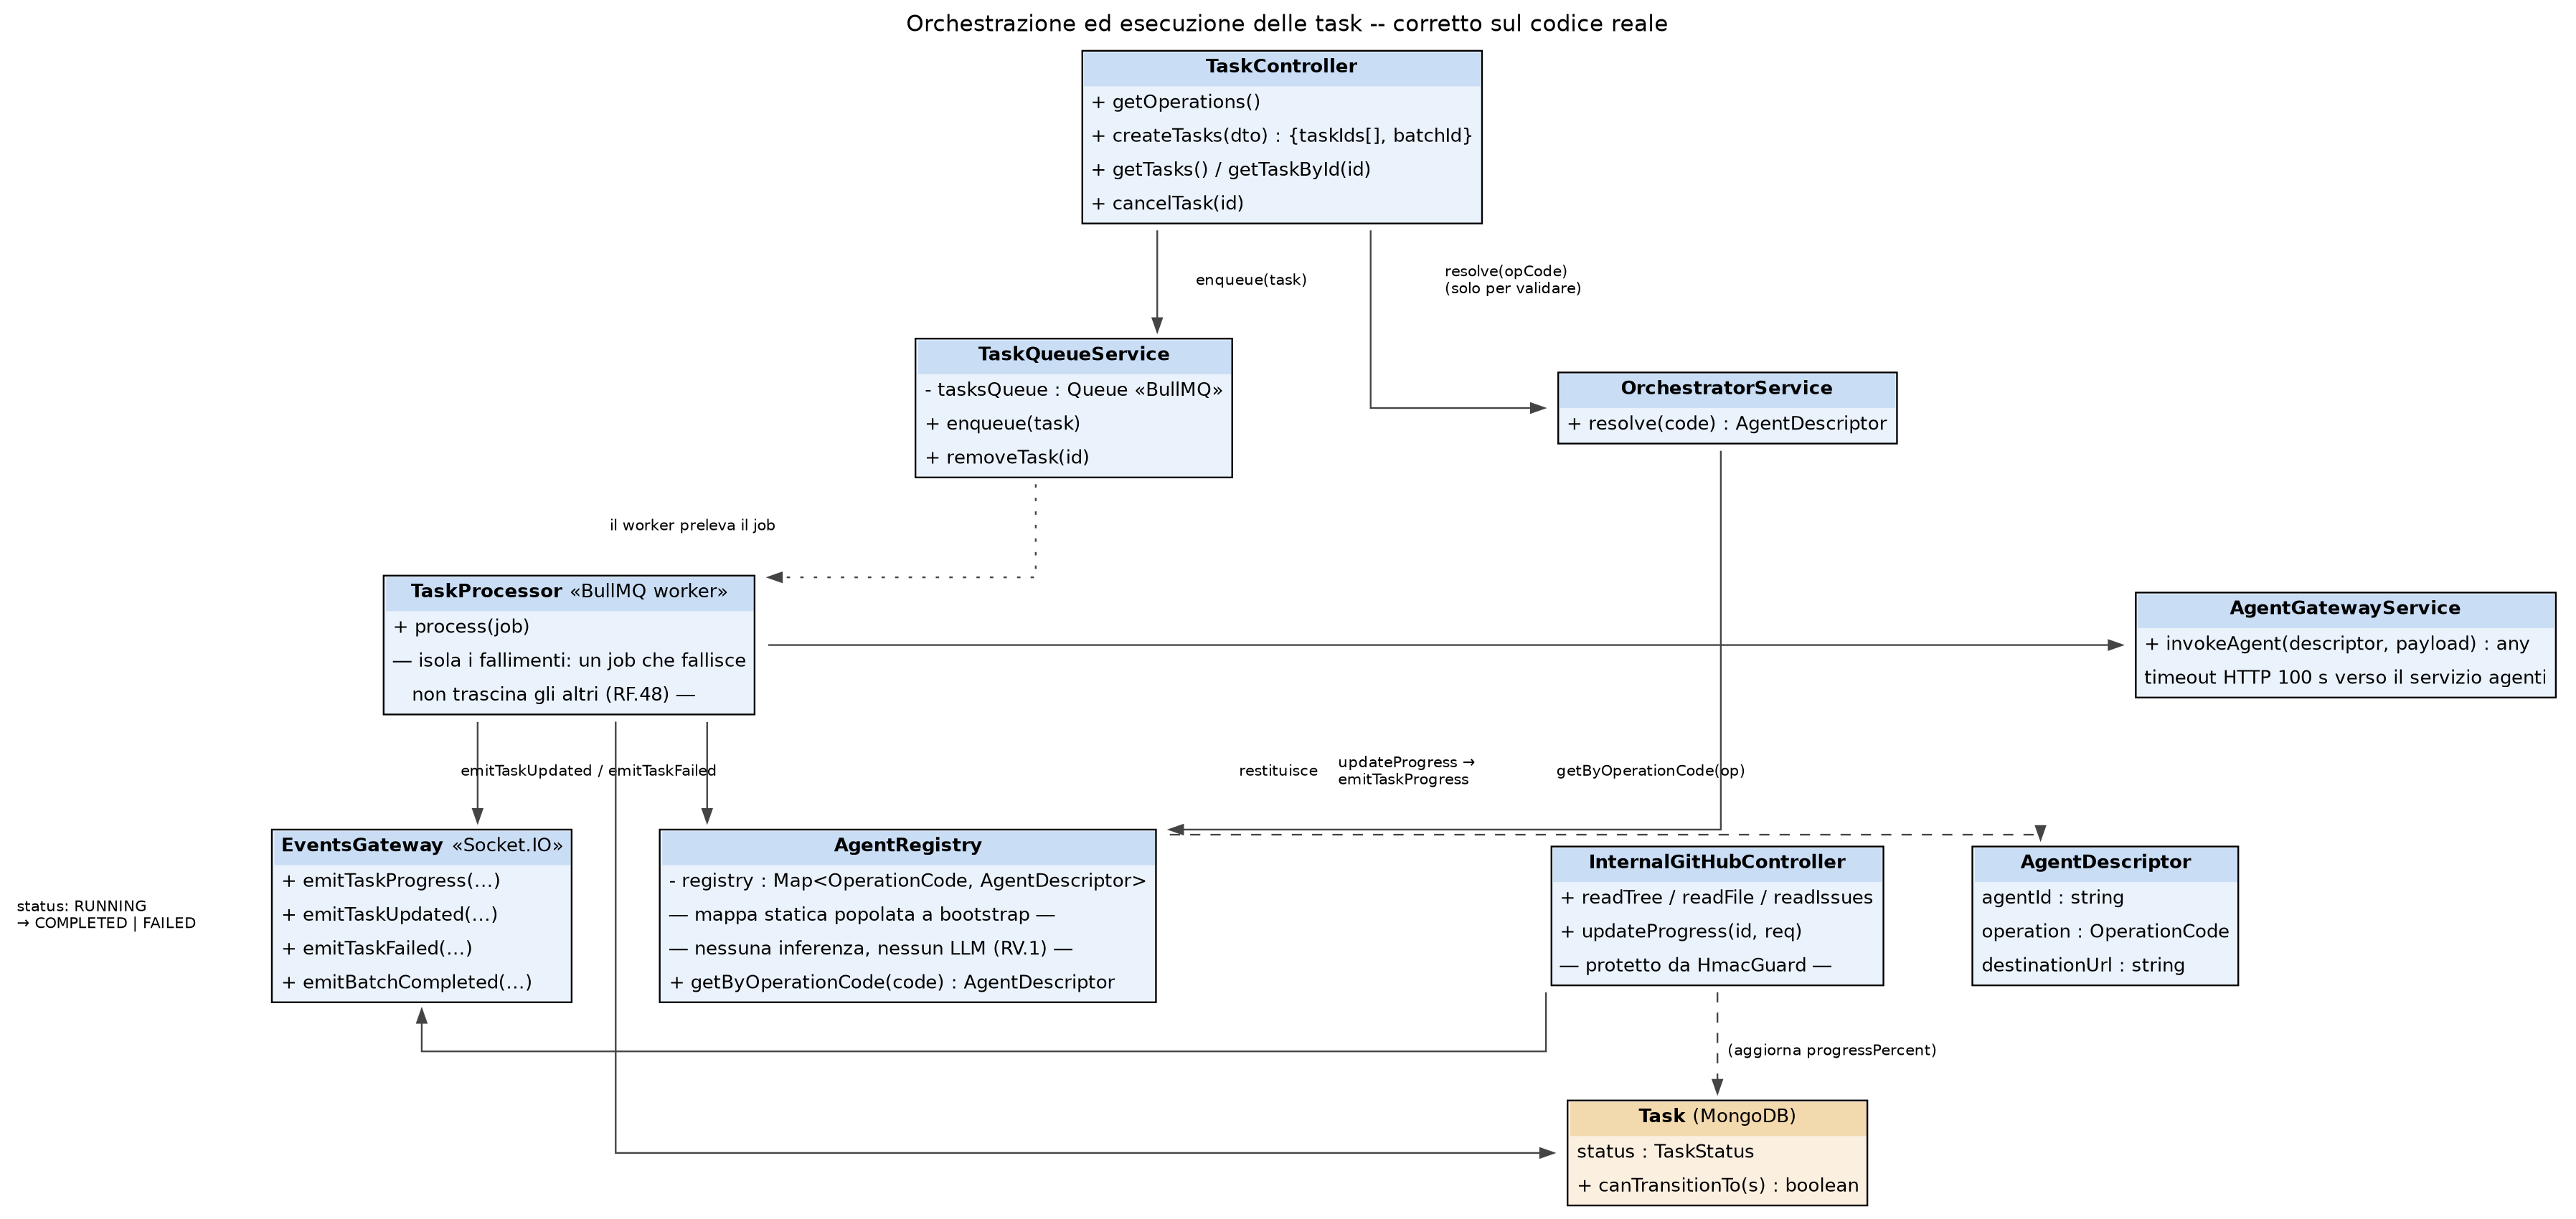
\includegraphics[width=0.98\textwidth]{figures/orchestratore.png}
\caption[Orchestrazione ed esecuzione]{Orchestrazione ed esecuzione. \texttt{AgentRegistry} è il cuore di RV.1 (mappa statica, nessun LLM). Il \texttt{TaskProcessor} isola i fallimenti: un job che fallisce non trascina gli altri (RF.48).}
\label{fig:orchestratore}
\end{figure}

\subsection{Ciclo di vita di una Task}

Una Task attraversa cinque stati (figura~\ref{fig:stati}): le transizioni ammesse sono solo quelle disegnate, e \texttt{Task.canTransitionTo()} rifiuta le altre. Nessuno stato terminale ha uscite: un rilancio è una Task nuova che tiene il riferimento alla precedente, così lo storico dei report resta interpretabile.

\begin{figure}[H]
\centering
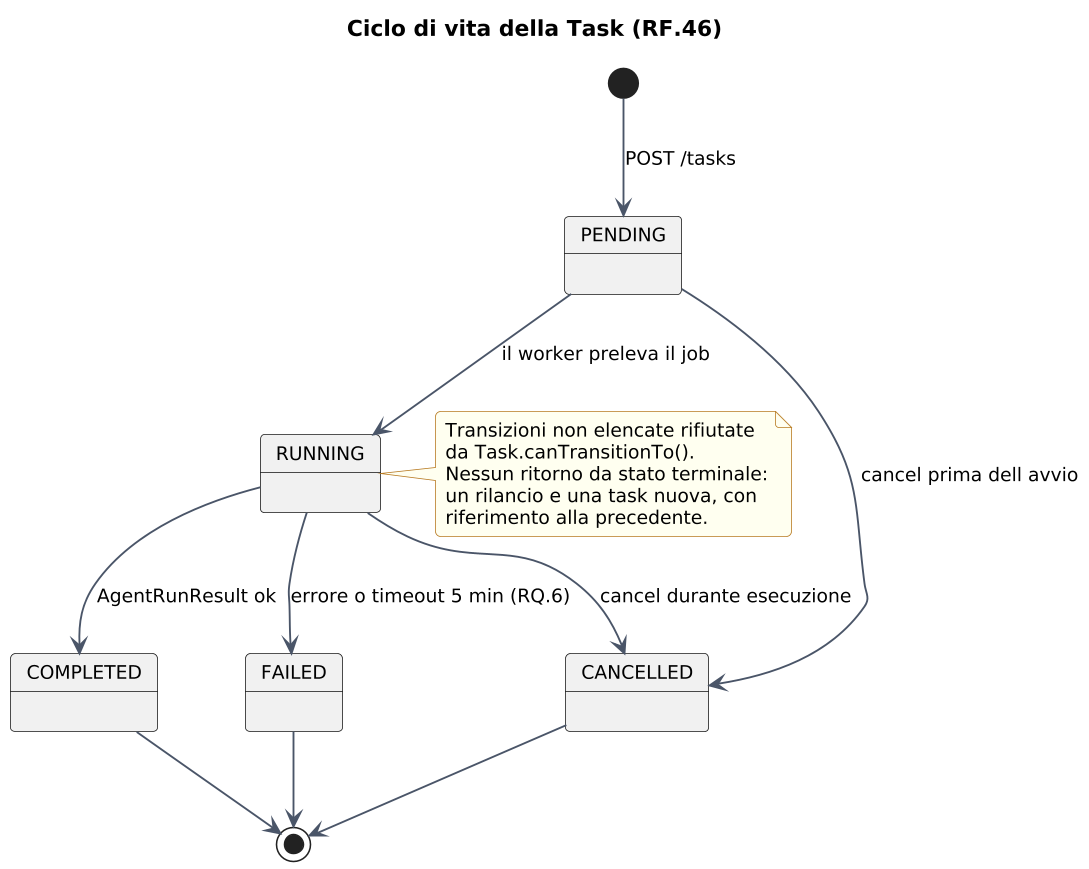
\includegraphics[width=0.72\textwidth]{figures/stati.png}
\caption[Ciclo di vita della Task]{Ciclo di vita della Task (RF.46). Il superamento del timeout globale del task (RQ.6, 5 minuti nell'implementazione PoC) porta a \texttt{FAILED} restando dentro il contratto \texttt{Report}. I timeout per-agente configurabili via variabile d'ambiente (\texttt{AGENT\_GATEWAY\_TIMEOUT\_DOCS\_S} / \texttt{AGENT\_\allowbreak{}GATEWAY\_\allowbreak{}TIMEOUT\_\allowbreak{}SECURITY\_S}, cfr.~\S~\ref{sub:adr3}) agiscono a livello di gateway e hanno valori inferiori (90 s per Docs e Changelog, 200 s per Security). Il diagramma mostra inoltre lo stato \texttt{CANCELLED} (annullamento esplicito da parte dell'utente).}
\label{fig:stati}
\end{figure}

Nel PoC questi cinque stati bastano perché nessun agente richiede input a metà esecuzione. L'MVP introduce l'agente Changelog con un flusso realmente interattivo (Sprint ID, esclusione di task con metadati insufficienti, conferma del Changelog di business): la Parte~\ref{part:frontend-spec} (\S~\ref{sec:fe-tasksstore}, figura~\ref{fig:fe-task-lifecycle}) estende questo stesso ciclo di vita con un campo \texttt{pendingInput}, una condizione sospensiva \emph{interna} allo stato \texttt{RUNNING} e non un sesto stato: i cinque stati qui sopra restano quindi l'unica fonte di verità sulle transizioni, anche nell'MVP.

\subsection{Il giro completo end-to-end}

La figura~\ref{fig:sequenza} mostra lo scambio di messaggi per un'operazione concreta (scansione OWASP su un repository privato). Il blocco centrale è quello su cui fermarsi in revisione: l'agente chiede l'albero, \emph{decide} di aprire un file, lo chiede, lo riceve. Nessuno di questi passi è programmato da noi: sono tool call scelte dal modello, e ognuna passa dal backend, che tiene il token e registra l'accesso. Un solo giro attraversa React, Vite, TanStack, NestJS, TypeScript, MongoDB, Redis, Python, LangGraph, Octokit, l'API GitHub, Docker, WebSocket e Swagger: è la dimostrazione di integrazione che le stesure precedenti non fornivano. Questo pattern di tool-calling guidato dal modello, qui illustrato sulla scansione OWASP, è specifico dell'agente Security: Docs e Changelog non lo attivano, perché il loro \texttt{ContextLoader} carica l'intero contesto necessario in un unico passo deterministico prima di interpellare il modello (\S~\ref{sec:scheletro-condiviso}).

\begin{figure}[H]
\centering
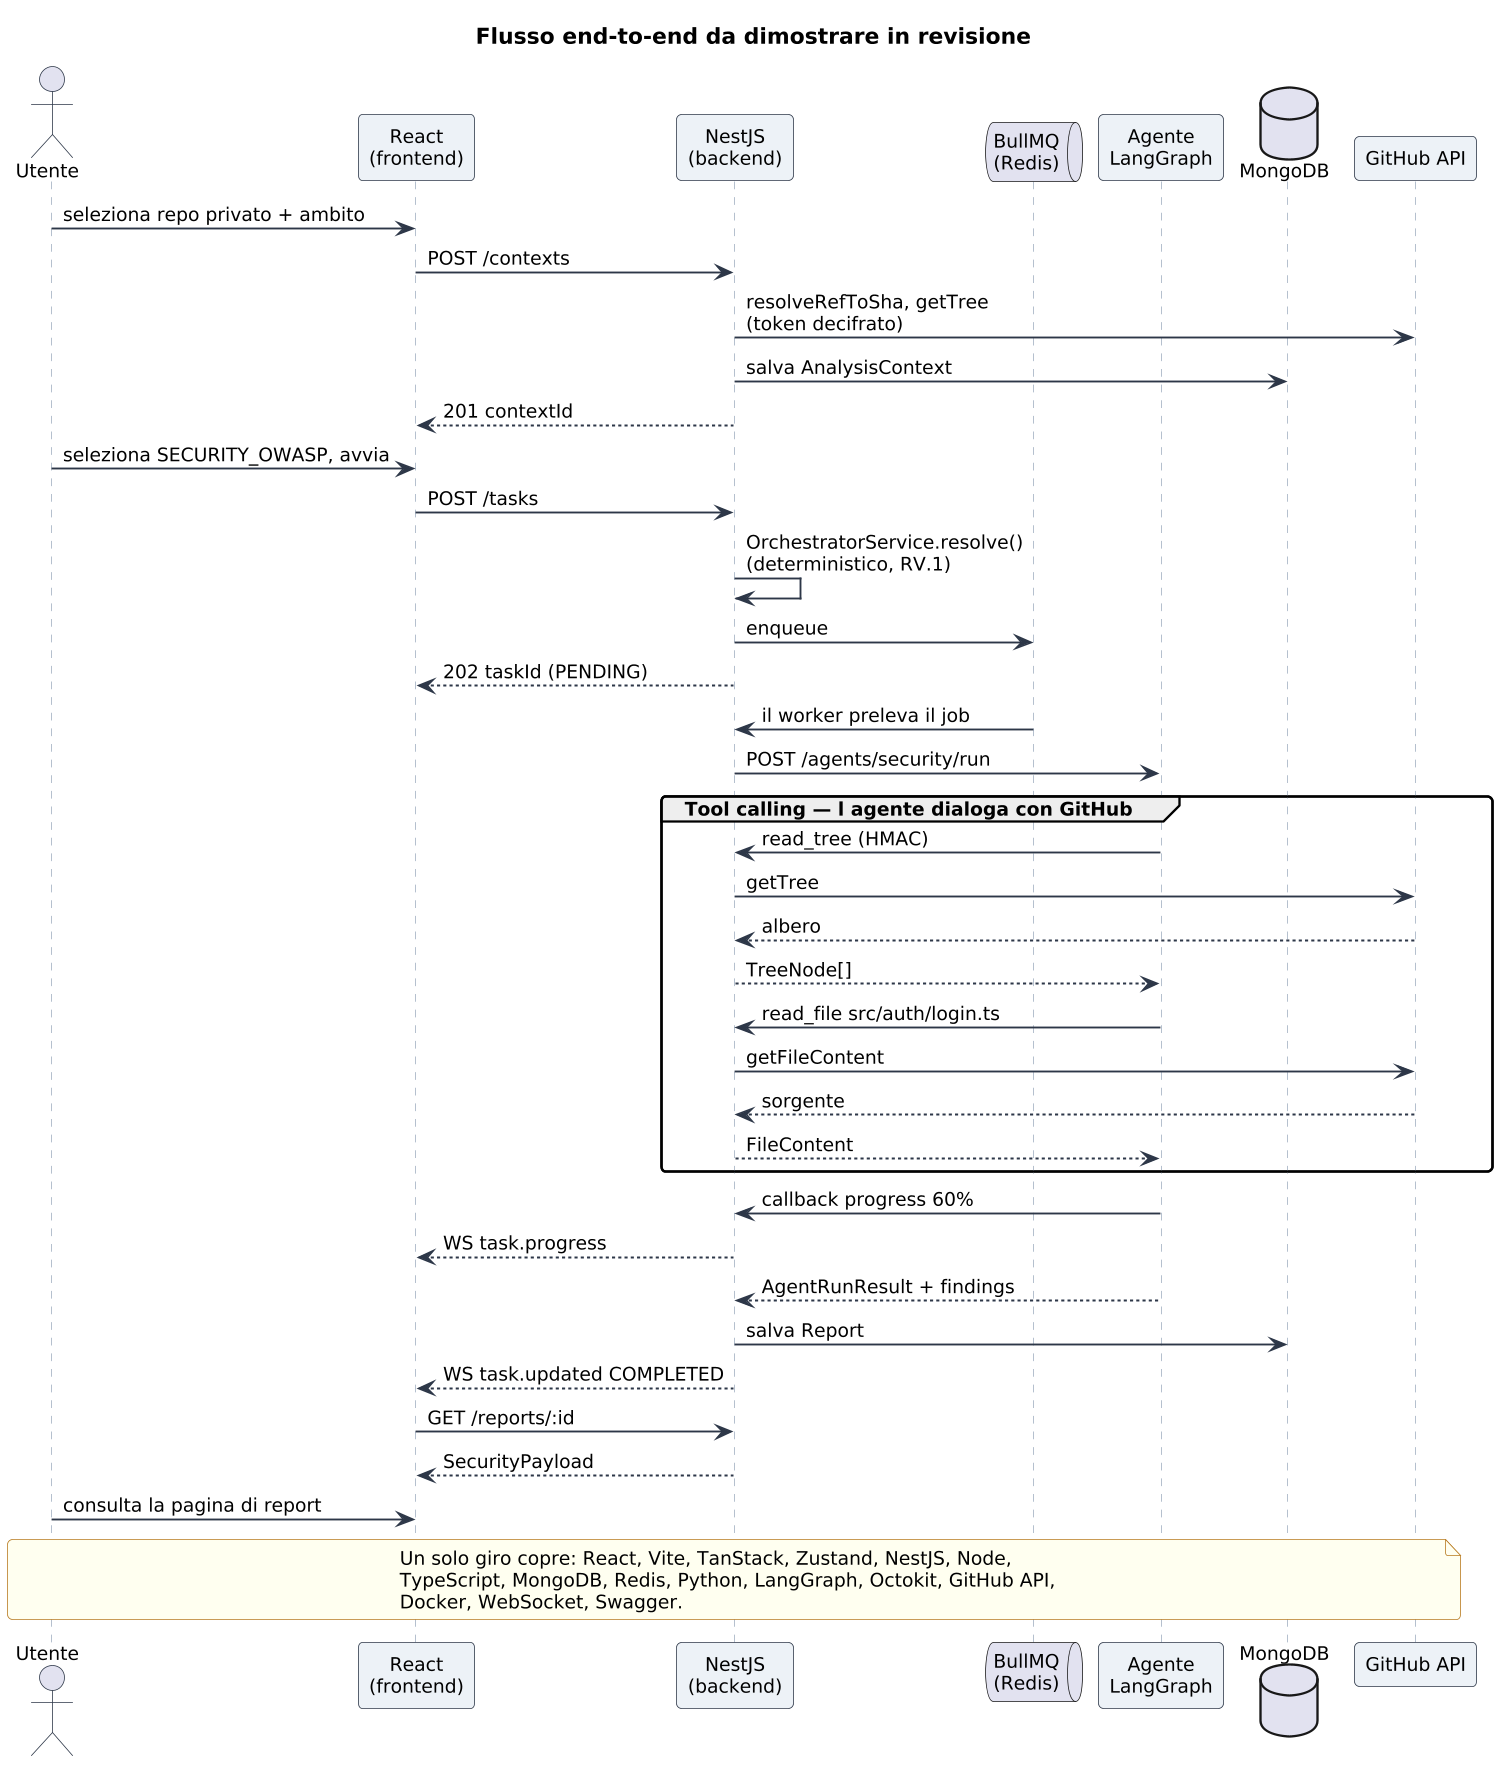
\includegraphics[width=0.86\textwidth]{figures/sequenza.png}
\caption[Giro completo end-to-end]{Sequenza end-to-end di una scansione. Il tool-calling dell'agente (blocco centrale) attraversa la facade GitHub, non GitHub direttamente.}
\label{fig:sequenza}
\end{figure}

\section{Cosa implemento per ciascun agente}

Poiché grafo, provider, envelope e gestione degli errori sono condivisi, ``implementare un agente'' significa scrivere sempre e solo tre cose: l'adattatore che carica il contesto (dai tool GitHub), il profilo con il suo template di prompt, e il parser che rilegge la risposta. L'esposizione via backend e la visualizzazione via frontend sono uguali per tutti e tre, scritte una sola volta contro il contratto \texttt{Report}. La figura~\ref{fig:agenti} mostra la gerarchia.

\begin{figure}[H]
\centering
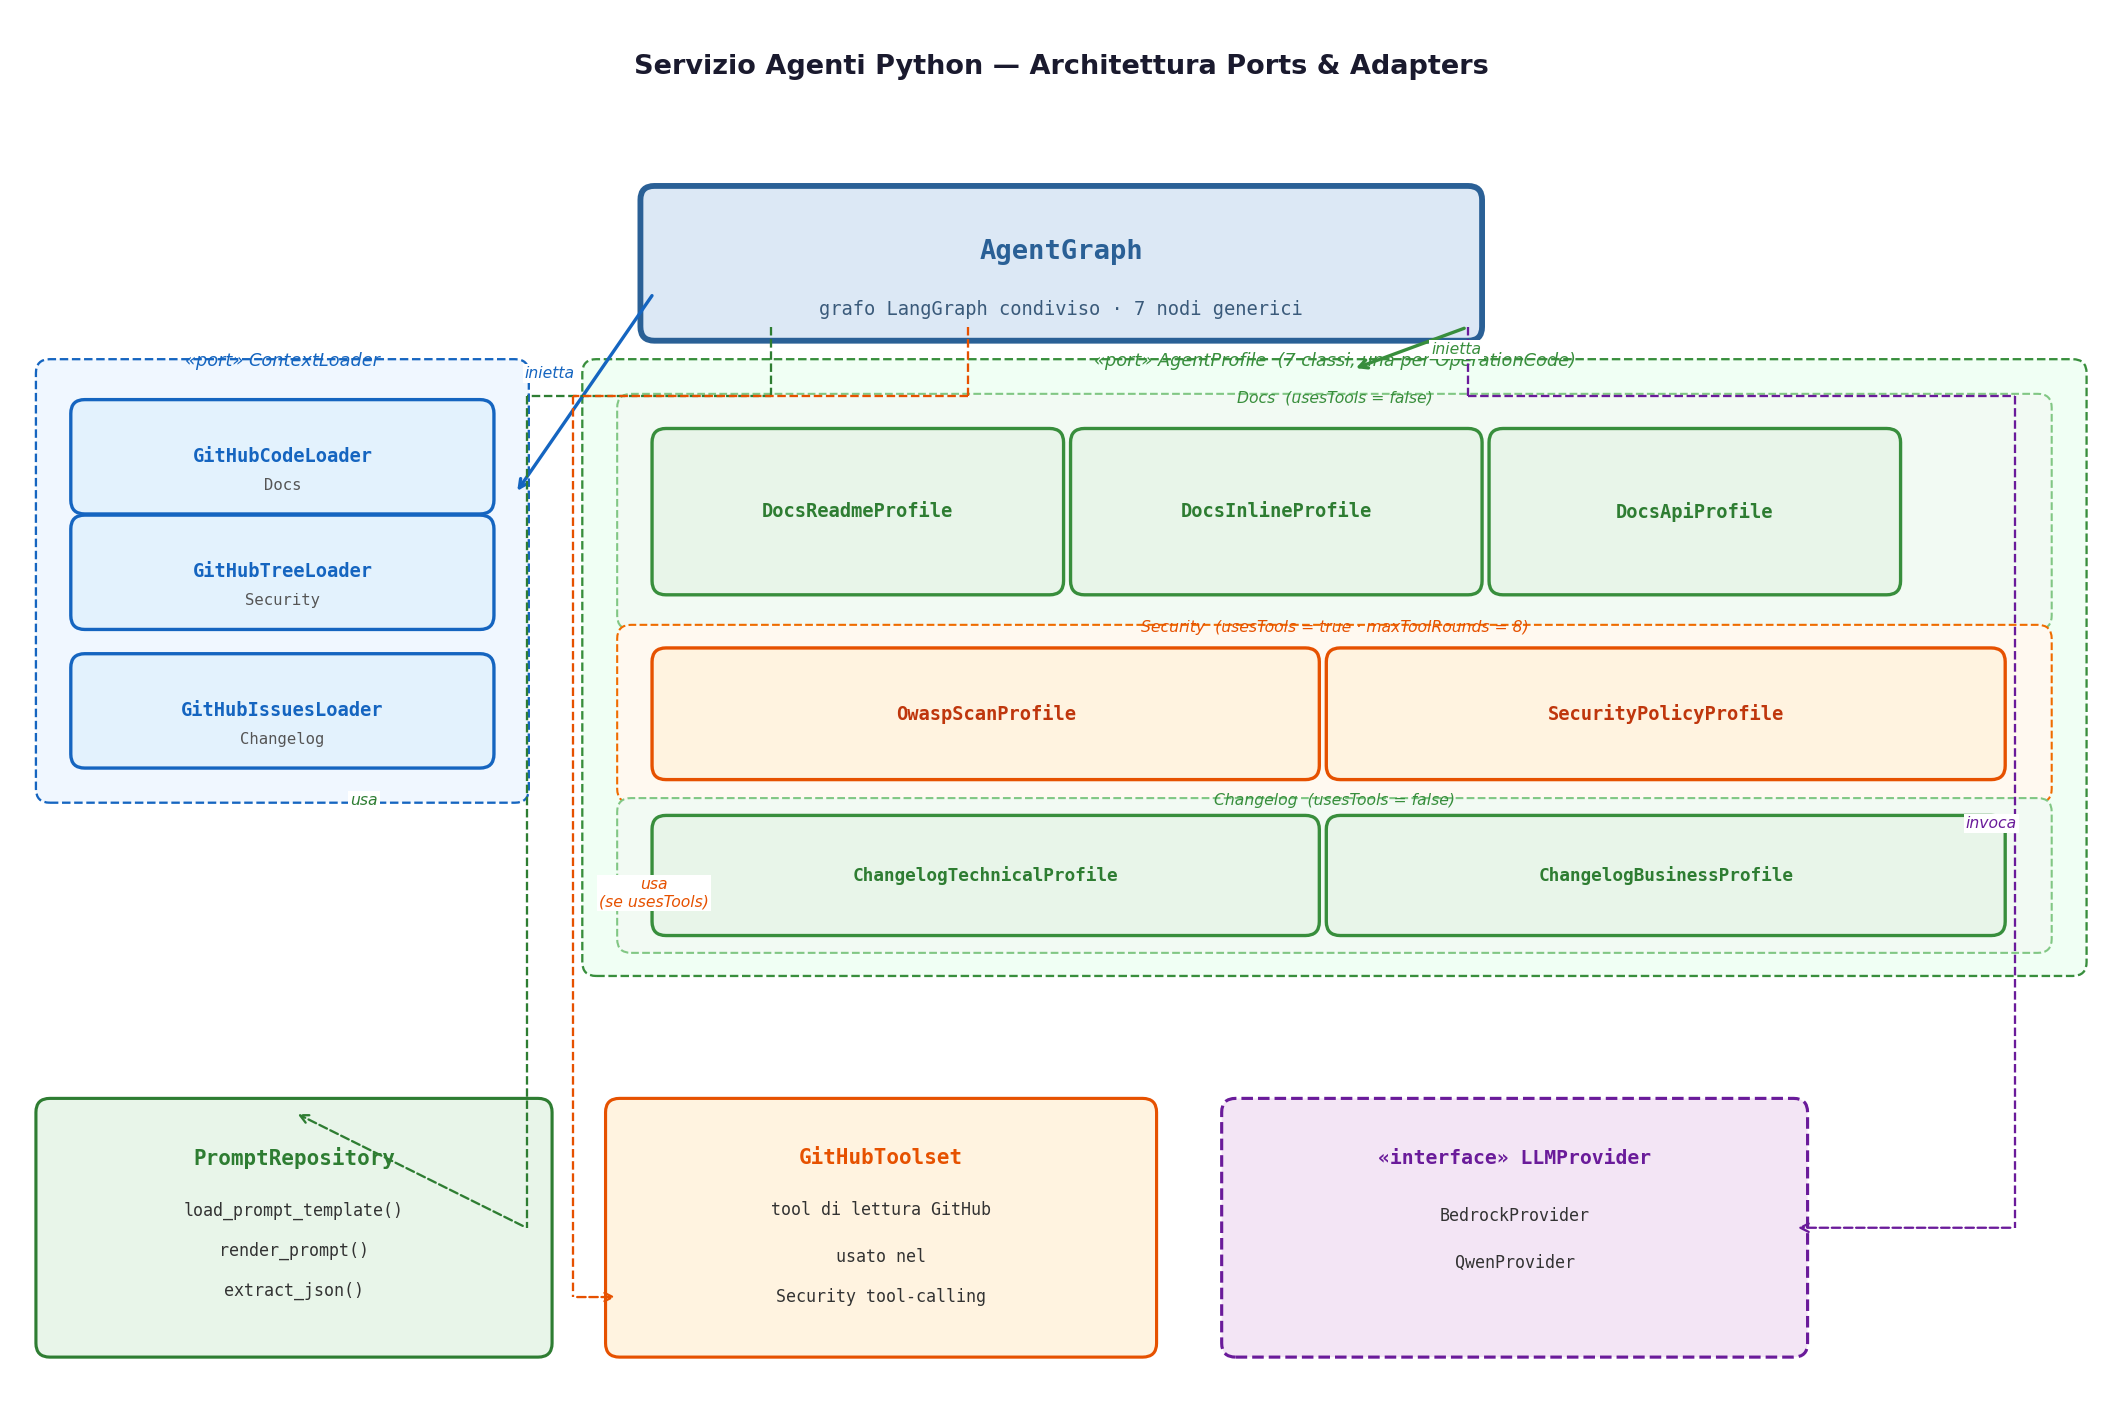
\includegraphics[width=\textwidth]{figures/agenti.png}
\caption[Servizio agenti Python]{Il servizio agenti. Il grafo LangGraph è unico e condiviso da tutti gli agenti (classe \texttt{AgentGraph}, sette nodi generici, cfr.~\S~\ref{sec:scheletro-condiviso}): non esiste un \texttt{build\_graph()} né un insieme di nodi distinto per sottoclasse. Ciò che varia per agente sono solo il \texttt{Loader} e il \texttt{Profile} iniettati (le porte descritte in \S~\ref{sec:scheletro-condiviso}). Il \texttt{PromptRepository} centralizza le funzioni di gestione dei prompt (\texttt{load\_prompt\_template}, \texttt{render\_prompt}, \texttt{extract\_json}), rendendo misurabile l'isolamento dei prompt (RQ.4); \texttt{GitHubToolset} espone i tool di lettura.}
\label{fig:agenti}
\end{figure}

\subsection{Agente Docs --- documentazione inline}

L'adattatore di contesto legge il codice dal repository \textbf{tramite i tool della facade} (\texttt{read\_tree}, \texttt{read\_file}), limitandosi all'ambito selezionato e ai soli linguaggi supportati. Prima di chiamare il modello c'è una piccola preparazione: attraversare quei file e individuare le unità che meritano documentazione (funzioni, classi, metodi) che ne sono prive o il cui commento è disallineato. Per un PoC non serve un analizzatore sintattico completo: basta riconoscere le definizioni senza un blocco di documentazione sopra. Il profilo carica il proprio template e vi inietta il codice di quelle unità, chiedendo al modello il commento nella convenzione corretta (JSDoc per TS/JS, docstring per Python). Il parser verifica che ogni commento sia ben formato e lo riaggancia a file e riga; il report è una \texttt{Proposal} di diff, mostrata nel frontend con una vista diff dedicata. Dove il codice è troppo intricato, l'agente emette un avviso strutturato invece di forzare un commento sbagliato.

\textbf{Implemento:} lettura del codice dall'ambito via facade, rilevamento delle unità non documentate, generazione del commento conforme, diff proposto, avviso per complessità eccessiva, visualizzazione del diff nell'interfaccia.\\
\textbf{Non implemento:} README di progetto e documentazione API (le altre due operazioni di Docs), e l'apertura effettiva della Pull Request.

\subsection{Agente Security --- scansione vulnerabilità OWASP}

L'adattatore di contesto usa gli stessi tool di lettura; nella variante policy-as-code legge in più il file \texttt{POLICY.md} alla radice. Qui non c'è pre-analisi: il codice dell'ambito, spezzato in porzioni che stanno nella finestra di contesto, va direttamente al modello. Il profilo carica il template di scansione, che istruisce il modello a cercare i pattern dell'OWASP Top 10 (SQL injection, cross-site scripting, segreti in chiaro, crittografia insicura, controllo accessi incompleto) e a restituire per ogni riscontro categoria, gravità, file e righe, spiegazione e rimedio. Il parser attende una risposta strutturata, la valida, normalizza la gravità sui livelli previsti e controlla i riferimenti alle righe; se la risposta è malformata scatta il ramo di parsing, se il modello è troppo lento quello di timeout, fissato per questo agente a 180 secondi (più ampio del default degli altri due, perché la scansione richiede più cicli di lettura file). Il report è una lista di \texttt{FindingBlock}, ciascuno con il suo rimedio, mostrata nel frontend come elenco filtrabile per gravità.

\paragraph{Scelta di \texttt{maxToolRounds = 8}.} Una scansione OWASP realistica non richiede di aprire l'intero repository: il modello esplora l'albero, individua i file ad alto rischio (entrypoint, gestione autenticazione, validazione degli input, configurazioni) e vi accede selettivamente. In pratica questo equivale a \textbf{4 coppie tool\_call/tool\_result} --- abbondantemente sufficienti per i pattern dell'OWASP Top 10 sui linguaggi supportati (TypeScript, JavaScript, Python). Il valore \textbf{8} bilancia tre vincoli in tensione:
\begin{itemize}
  \item \emph{Copertura}: 8 round consentono di ispezionare tra 4 e 6 file significativi con margine per revisitarne uno; scendere sotto 4 rischierebbe di non coprire percorsi di esecuzione critici.
  \item \emph{Budget di token}: \texttt{Qwen3-Coder-30B-A3B-Instruct} ha una finestra nativa di $\sim$32 K token. Ogni coppia tool\_call/tool\_result produce in media 1.500--2.000 token di overhead (richiesta strutturata + risposta dell'agente); 8 round aggiungono quindi $\sim$12--16 K token alla cronologia, compatibili con il \texttt{max\_scope\_chars} di 60.000 caratteri fissato in \S~\ref{sec:domain-model} e con il margine riservato al system prompt e alla risposta finale.
  \item \emph{Timeout}: 8 round completano ampiamente entro i 180 secondi del timeout interno, anche tenendo conto della latenza di rete verso la facade GitHub e dei tempi di inferenza del modello.
\end{itemize}
Il valore è esposto come variabile d'ambiente (\texttt{MAX\_TOOL\_ROUNDS=8}) e va trattato come punto di partenza: se la validazione sul golden set del Piano di Qualifica mostrasse che la copertura è insufficiente, basta alzare l'env var senza rilascio del codice.

\textbf{Implemento:} estrazione del codice via facade, scansione OWASP Top 10, output strutturato (categoria/gravità/posizione/rimedio), gestione di timeout e parsing, elenco dei finding nell'interfaccia. In opzione, la variante policy-as-code su \texttt{POLICY.md}, che riusa identico il grafo cambiando solo il template.\\
\textbf{Non implemento:} copertura esaustiva dell'intera OWASP Top 10 e applicazione automatica dei rimedi --- l'agente segnala, è il Security Auditor a validare.

\subsection{Agente Changelog --- changelog tecnico}

Rispetto alle stesure precedenti, l'adattatore di contesto \textbf{non} legge più una fixture JSON: interroga \textbf{GitHub Issues dal vivo} tramite il tool \texttt{read\_issues}, recuperando le storie di uno Sprint (titolo, descrizione, criteri di accettazione, stato, etichette, milestone). Il lavoro prima del modello è interno: filtrare le issue effettivamente chiuse per lo Sprint indicato e poi passarle al controllo di qualità dei metadati, che mette da parte quelle con descrizione vuota o troppo povera. Si segue il percorso ``procedi escludendo'': si registra quali task sono state scartate e si prosegue solo con quelle valide, così il report è onesto su cosa copre. Il profilo carica il template del changelog tecnico e chiede al modello un resoconto per sviluppatori in Markdown; siccome l'output è prosa, la validazione è più lieve, e il testo viene arricchito con i collegamenti ai ticket. Il report è composto da un unico \texttt{TextBlock} in Markdown, generato dal modello, che contiene già tutte le voci incluse con i link ai ticket; gli eventuali \texttt{ChangelogItemBlock} che seguono non sono altre voci del changelog, ma l'elenco --- per trasparenza --- delle issue \emph{escluse} dal cancello di qualità sui metadati. Il tutto è mostrato nel frontend come Markdown renderizzato, con la lista delle esclusioni in coda.

\textbf{Implemento:} lettura delle issue da GitHub dal vivo, filtro delle chiuse, cancello di qualità sui metadati (scarto delle povere), sintesi tecnica in Markdown, arricchimento con i link ai ticket, rendering Markdown nell'interfaccia.\\
\textbf{Non implemento:} il changelog di business (sarebbe un nodo in più che rigira il testo tecnico in un secondo prompt).

\subsection{Il filo comune}

In tutti e tre i casi l'unica cosa che scrivo davvero di nuovo, lato agente, è ``da dove leggo'' (quale tool della facade) e ``cosa chiedo e come rileggo la risposta''. Orchestrazione dei nodi, chiamata al modello con timeout, forma del report e gestione degli errori arrivano dallo scheletro condiviso. A questo si aggiunge il filo comune lato stack applicativo: gli endpoint REST, la persistenza su MongoDB e i componenti dell'interfaccia che mostrano il \texttt{Report} sono scritti una sola volta e riusati identici, perché tutti parlano lo stesso contratto.

\paragraph{Nota implementativa --- 7 classi \texttt{AgentProfile}, una per \texttt{OperationCode}.}
Il listing di composizione degli adapter mostra tre righe (Docs, Security, Changelog), ma in implementazione il numero di classi \texttt{AgentProfile} è \textbf{sette} --- una per ciascun valore di \texttt{OperationCode}:

\begin{center}
\small
\texttt{DocsReadmeProfile} · \texttt{DocsInlineProfile} · \texttt{DocsApiProfile} ·
\texttt{OwaspScanProfile} · \texttt{SecurityPolicyProfile} ·
\texttt{ChangelogTechnicalProfile} · \texttt{ChangelogBusinessProfile}
\end{center}

La scelta di 7 classi distinte invece di 3 profili parametrizzati è motivata dalla struttura stessa dell'interfaccia \texttt{AgentProfile}: i metodi \texttt{build\_prompt()} e \texttt{parse\_output()} hanno implementazioni \emph{genuinamente diverse} per ciascuna operazione --- il prompt per generare un README differisce strutturalmente da quello per documentare API REST; il parser di \texttt{FindingBlock} OWASP differisce da quello di \texttt{PolicyViolationBlock}. Aggregare operazioni diverse in un solo profilo parametrizzato produrrebbe catene \texttt{if/elif} su \texttt{operation} dentro ogni metodo, violando il principio di singola responsabilità e rendendo i test per operazione più fragili. Con 7 classi invece:

\begin{itemize}
  \item Il dispatch \texttt{OperationCode} $\to$ \texttt{AgentProfile} è una mappa statica in \texttt{AgentRegistry}, con zero logica condizionale nei profili stessi.
  \item Ogni profilo si testa in isolamento iniettando un provider LLM simulato, il che è essenziale per validare la copertura del golden set (PdQ).
  \item Aggiungere una nuova operazione significa aggiungere un file, non modificare classi esistenti (Principio Open/Closed).
  \item Il collegamento profilo $\to$ template di prompt nel \texttt{PromptRepository} è verificabile a colpo d'occhio: \texttt{docs/\allowbreak{}readme.txt}\penalty0\ $\to$ \texttt{DocsReadmeProfile}, \texttt{security/\allowbreak{}owasp.txt}\penalty0\ $\to$ \texttt{OwaspScanProfile}, ecc.
\end{itemize}

I tre ``agenti'' del listing restano l'unità concettuale corretta (Docs, Security, Changelog condividono rispettivamente \texttt{Loader} e comportamento \texttt{usesTools}); i 7 profili sono la granularità implementativa, invisibile al grafo LangGraph condiviso che li riceve già istanziati.

\section{Decisioni architetturali (ADR)}
\label{sec:adr}

Queste decisioni sono vincolanti per l'implementazione: sono i punti dove la strada più comoda viola un requisito. Gli sviluppatori le seguano anche quando una scorciatoia sembra allettante.

\paragraph{ADR-1 --- Il token GitHub non lascia NestJS.} Gli agenti devono dialogare con GitHub, ma RS.3 vieta loro la scrittura e RS.2 impone token cifrati. \textbf{Decisione}: facade read-only su NestJS, esposta agli agenti come tool LangGraph. Il token resta cifrato nel backend; l'agente decide cosa leggere e itera, ma ogni chiamata passa dalla whitelist. \textbf{Da non fare}: passare il token al servizio Python perché ``è più semplice''. Sposterebbe il segreto oltre un secondo confine e renderebbe RS.3 da verificare in due codebase.

\paragraph{ADR-2 --- L'LLM dietro una porta, fornitore della famiglia di Bedrock.} Credenziali AWS assenti. \textbf{Decisione}: \texttt{LLMProvider} con implementazione attiva verso API gestita della stessa famiglia di modelli che useremo su Bedrock, e \texttt{BedrockProvider} scritto ma non attivo. \textbf{Da non fare}: eseguire un modello locale, che non direbbe nulla di utile sul prodotto e costringerebbe a ritarare i prompt.

\paragraph{ADR-3 --- Coda per l'esecuzione, non chiamata sincrona.}\label{sub:adr3} RQ.6 fissa a $\leq 5$ minuti il tempo di risposta per l'esecuzione di un singolo agente, e i fallimenti vanno isolati (RF.48). Il timeout interno dell'agente è configurato a \textbf{90 secondi} per Docs e Changelog e a \textbf{180 secondi} per Security (che itera più cicli di lettura file via tool-calling): entrambi i valori restano ampiamente entro il limite di RQ.6; l'ottimizzazione di prompt e numero di letture nelle fasi successive resta utile per contenere costi e tempo percepito, non per rientrare in un vincolo già rispettato.

Il timeout HTTP del gateway (\texttt{AgentGatewayService}) è configurato \textbf{per operation code} per garantire che non si chiuda prima del timeout interno dell'agente: \textbf{90 s} per le operazioni Docs e Changelog, \textbf{200 s} per le operazioni Security (10 s di margine rispetto al timeout interno di 180 s). Il valore è letto da variabile d'ambiente (\texttt{AGENT\_GATEWAY\_TIMEOUT\_DOCS\_S} / \texttt{AGENT\_GATEWAY\_TIMEOUT\_SECURITY\_S}), così cambia la configurazione, non il codice. \textbf{Decisione}: \texttt{POST /tasks} accoda e ritorna subito; un worker esegue; gli aggiornamenti arrivano via WebSocket. \textbf{Da non fare}: eseguire l'agente dentro il ciclo della richiesta HTTP, che accoppierebbe l'interfaccia ai tempi del modello.

\paragraph{ADR-4 --- Gli artefatti degli agenti sono proposte, non modifiche.} \textbf{Decisione PoC}: l'output è un \texttt{Report} immutabile scaricabile, mai un commit. Il token richiesto ha scope di sola lettura. \textbf{Aggiornamento MVP}: l'apertura della Pull Request è delegata al \emph{backend} NestJS (ADR-AWS-10, \S~\ref{sec:aws-adr}), non all'agente --- che rimane read-only. L'umano che esercita la supervisione richiesta da ADR-4 è l'utente che clicca \emph{Applica} nella UI del report, avviando la chiamata verso il backend che apre la PR; il \emph{merge} resta poi un atto distinto, condotto dall'utente direttamente su GitHub. Non esiste un endpoint \texttt{/apply} separato: il backend apre la PR immediatamente al completamento del task, e il link alla PR viene reso disponibile nella pagina del report (ADR-FE-1). Il token GitHub nell'MVP richiede scope di scrittura (\texttt{repo}), ma resta esclusivo del backend.

Queste quattro ADR sono le uniche vincolanti per il PoC e per l'orchestrazione minima (\S~\ref{sec:orchestratore}). Quattro decisioni ulteriori (ADR-5--ADR-8), relative al componente di \emph{orchestratore di produzione} proposto per una fase successiva al MVP, sono presentate in \S~\ref{sub:orch-adr}, subito dopo la descrizione del componente a cui si riferiscono (\texttt{BatchStep}, \texttt{RetryPolicy\allowbreak{}Engine}, \texttt{Circuit\allowbreak{}Breaker\allowbreak{}Service}, \texttt{Agent\allowbreak{}Pool\allowbreak{}Manager}), invece che qui, per non costringere chi legge a memorizzare nomi di classi non ancora introdotte.

\section{Come validiamo il PoC}

Il PoC si aggancia direttamente alle metriche del Piano di Qualifica.

L'\textbf{accuratezza} (obiettivo $>85\%$) si misura preparando un piccolo golden set di file con vulnerabilità note e confrontando l'output dell'agente Security. Con il provider via API gestita, questa metrica va verificata presto sul fornitore effettivamente scelto.

Il \textbf{tempo di risposta} si misura per singola esecuzione, dall'invocazione dell'endpoint REST alla disponibilità del report, e include l'overhead di persistenza su MongoDB e delle letture GitHub (mitigate dalla cache). \textit{Nota di coerenza (verificata sull'Analisi dei Requisiti v1.0.0):} RQ.6 fissa il vincolo a $\leq 5$ minuti (Obbligatorio, fonte UC27.2/PdQ MPD 12), come già riportato nella Tabella~\ref{tab:aws-req-decisioni}. I timeout attualmente configurati nel PoC (90 s per Docs e Changelog, 180 s per Security) restano quindi ampiamente \emph{sotto} quella soglia vincolante, non sopra: il target interno più stringente che il team si è dato in fase di ottimizzazione va visto come un margine di sicurezza aggiuntivo da mantenere stretto per l'esperienza utente (\S~\ref{sec:orchestratore}, RQ.10), non come un vincolo di RQ.6 ancora da rispettare.

L'\textbf{isolamento dei prompt} è verificabile per costruzione, perché i prompt sono file esterni. Conviene aggiungere un test statico che fallisce se un modulo agente contiene literal di stringa oltre una soglia: rende la metrica MPD\_14 una prova automatica.

La \textbf{copertura dei test} è raggiungibile perché sia \texttt{LLMProvider} sia la facade GitHub sono dietro interfaccia: nei test si iniettano un provider simulato e un client GitHub finto con risposte registrate, così i test girano offline, deterministici e a costo zero.

Si aggiunge la verifica dell'\textbf{integrazione end-to-end}: un test che, partendo da una chiamata simulata dal frontend, verifica che il backend instradi correttamente l'agente, che l'agente legga via facade (con client GitHub finto), che il report sia persistito su MongoDB e restituito nel formato atteso.

\paragraph{Uso dei dati per l'addestramento (RS.5).} Il vincolo RS.5 impone di garantire che il codice sorgente inviato al modello \textbf{non venga trattenuto né usato per addestrare modelli di terzi}. Questo punto merita attenzione perché, con la scelta di un'API gestita, la garanzia dipende dal fornitore e dal canale, e i due canali che il progetto usa in momenti diversi \textbf{non offrono la stessa copertura in modo automatico}.

Quando il modello sarà servito da \textbf{AWS Bedrock}, in produzione, la copertura è netta: AWS dichiara che i dati dei clienti non vengono mai usati per addestrare i modelli sottostanti, e questo vale anche per i modelli open-weight di terzi serviti tramite Bedrock, perché l'inferenza avviene nel perimetro AWS. In quella configurazione RS.5 è soddisfatto dai termini del servizio.

Durante il \textbf{PoC}, però, il modello non passa da Bedrock ma dall'\textbf{API diretta del fornitore} (nel nostro esempio, DashScope di Alibaba Cloud): la garanzia di Bedrock non si estende a questo canale, che è retto dai propri termini di servizio. La documentazione dei fornitori è esplicita nel rimandare le politiche sui dati al provider effettivamente usato. Ne consegue un adempimento preciso, non tecnico ma con scadenza esterna, da svolgere \textbf{prima} di inviare al modello il primo file di un repository privato del proponente:
\begin{enumerate}
  \item verificare, nei termini del piano API scelto (per Qwen: il piano DashScope internazionale, regione di Singapore/Model Studio), la clausola specifica sulla ritenzione dei dati e sul loro eventuale uso per addestramento, controllando se esista un'opzione o un tier che escluda esplicitamente tale uso;
  \item mettere a verbale l'esito della verifica, con data e versione dei termini consultati, perché è la forma in cui RS.5 è dimostrabile in sede di collaudo;
  \item tracciare il requisito nel Piano di Qualifica come \textbf{controllo documentale}, non come test automatico: nessun test può dimostrare che un terzo non usi i dati, solo i termini contrattuali possono.
\end{enumerate}
Se la verifica sui termini dell'API diretta non desse garanzie sufficienti, l'alternativa a costo maggiore è anticipare l'uso di un canale con garanzie enterprise sui dati (Bedrock stesso, se e quando le credenziali arrivano, o un intermediario equivalente), accettando però che questo tolga al PoC la sua indipendenza dalle credenziali AWS. È una decisione da prendere consapevolmente, non un dettaglio da rimandare.

\section{Estensioni di scalabilità dell'orchestratore (roadmap oltre l'MVP)}
\label{sec:orchestratore-produzione}

\textbf{Precisazione terminologica.} L'\emph{Orchestratore} richiesto da RV.1 --- lo smistamento deterministico delle operazioni verso gli agenti, senza LLM nella logica di instradamento --- \textbf{è interamente implementato ed è parte del perimetro valutato per l'MVP}, non di questa roadmap. Nel PoC, \texttt{AgentRegistry} risolve un \texttt{OperationCode} nel proprio agente con una mappa statica e \texttt{TaskProcessor} esegue le Task isolandone i fallimenti (RF.48); nell'MVP questa stessa coppia di componenti resta l'unico orchestratore in esecuzione ed è completata dalla dashboard di monitoraggio del Frontend MVP (RF.43--RF.47, Parte~\ref{part:frontend-spec}), che ne rende visibile in tempo reale lo stato delle Task. È questo insieme --- instradamento deterministico (\S~\ref{sec:orchestratore}) più dashboard (Parte~\ref{part:frontend-spec}) --- a soddisfare RV.1 e RF.40--RF.48, ed è questo insieme a essere oggetto di valutazione per l'MVP.

Quello che \textbf{questa sezione} progetta non è quindi ``l'orchestratore'', ma un insieme di \emph{estensioni di scalabilità e resilienza} che l'orchestratore minimo non regge in un prodotto a pieno carico: incatenare più operazioni con dipendenze, ritentare automaticamente un fallimento transitorio, distribuire il carico su più istanze del servizio agenti, dare a chi supervisiona un quadro d'insieme operativo dedicato (batch, code, pool, circuit breaker, distinto dalla dashboard utente della Parte~\ref{part:frontend-spec}). Il disegno mantiene due vincoli ereditati dal PoC/MVP: l'instradamento resta deterministico (RV.1) e il contratto \texttt{Report}/\texttt{Task} non cambia forma, così il frontend esistente continua a funzionare senza riscritture.

\textbf{Nota di perimetro.} Quanto segue è un disegno architetturale, non una specifica implementata: i suoi requisiti (\S~\ref{sub:orch-requisiti}) non sono ancora nel registro ufficiale e restano al di fuori del perimetro dell'MVP descritto nella Parte~\ref{part:frontend-spec} (Frontend) e nella Parte~\ref{part:aws-manuale} (Infrastruttura AWS): nessuna delle due usa \texttt{BatchStep}, \texttt{AgentPoolManager} o i circuit breaker qui definiti --- l'MVP resta sull'orchestrazione minima di \S~\ref{sec:orchestratore} (\texttt{AgentRegistry}/\texttt{TaskProcessor}, \texttt{Desired Count: 1} su ECS Fargate, nessun pool di istanze), che è a tutti gli effetti \emph{l'Orchestratore dell'MVP}, non un suo sostituto provvisorio. Il componente qui descritto è collocato a chiusura della Parte~\ref{part:poc} perché estende direttamente l'orchestrazione minima e le ADR-1--ADR-4 del PoC/MVP; va letto come roadmap per l'evoluzione oltre l'MVP, da formalizzare con il proponente prima di essere pianificato in una release.

\subsection{Obiettivo e perimetro}

L'orchestratore di produzione sostituisce la coppia \texttt{AgentRegistry}/\texttt{TaskProcessor} con un insieme di componenti cooperanti che rispondono a quattro esigenze lasciate fuori dal PoC:

\begin{itemize}
    \item \textbf{Batch complessi}: un batch non è più un insieme di operazioni indipendenti avviate insieme, ma un grafo diretto aciclico (DAG) di passi con dipendenze --- ad esempio, ``esegui Security, e solo se non emergono finding \texttt{critical} esegui Docs sugli stessi file''.
    \item \textbf{Resilienza}: un fallimento transitorio (timeout di rete verso GitHub, errore 5xx del provider LLM) non deve richiedere un nuovo avvio manuale, ma un retry automatico e limitato.
    \item \textbf{Scaling}: il servizio agenti Python deve poter girare in più istanze, con il carico distribuito tra loro e senza che una singola istanza sovraccarica diventi un collo di bottiglia.
    \item \textbf{Osservabilità}: chi gestisce il sistema deve vedere, in tempo reale, quanti batch sono in corso, dove si sono fermati, quali agenti sono in salute e quali soglie di errore si stanno avvicinando.
\end{itemize}

Restano fermi, ereditati dal PoC: l'invarianza del contratto \texttt{Report} (\S~\ref{sec:contratto}), la separazione tra API pubbliche e interne (\S~\ref{sec:api}), il vincolo che il token GitHub non lasci il backend (ADR-1) e l'astrazione \texttt{LLMProvider} (ADR-2). L'orchestratore non introduce un nuovo linguaggio né un nuovo datastore: resta su NestJS, MongoDB, Redis e BullMQ, coerentemente col principio di minimizzare le variabili tecnologiche nuove (\S~\ref{sec:tecnologie}).

\subsection{Requisiti}
\label{sub:orch-requisiti}

I requisiti che seguono \textbf{non sono ancora presenti nel registro dei requisiti} (RF.1--RF.105, RQ.1--RQ.11, RS.1--RS.5, RV.1--RV.21): descrivono capacità di produzione (batch come DAG, retry, circuit breaker, scaling, dashboard estesa) che il registro attuale non copre, perché il registro si ferma al perimetro del MVP e questa sezione guarda oltre. I codici proseguono la numerazione esistente per evitare collisioni (RF.106+, RQ.12+, RS.6) e vanno intesi come una \textbf{proposta} da sottoporre al proponente e formalizzare nel registro prima di essere trattati come requisiti vincolanti.

\begin{table}[H]
\centering
\caption{Requisiti aggiuntivi dell'orchestratore di produzione.}
\label{tab:orch-requisiti}
\vspace{2mm}
\renewcommand{\arraystretch}{1.3}
\begin{tabularx}{\textwidth}{|c|X|}
\hline
\textbf{Codice} & \textbf{Descrizione} \\ \hline
RF.106 & Un Batch è definito come DAG di passi (\texttt{BatchStep}), ciascuno con zero o più dipendenze verso altri passi dello stesso batch. \\ \hline
RF.107 & Una Task fallita per errore classificato come transitorio (RS.6, sotto) viene ritentata automaticamente secondo una \texttt{RetryPolicy} configurabile per operazione. \\ \hline
RF.108 & Il carico verso il servizio agenti è distribuito su più istanze registrate in un pool, senza affinità tra Task e istanza. \\ \hline
RF.109 & Una dashboard mostra, in tempo reale, lo stato dei batch attivi, la profondità delle code, la salute del pool di agenti e lo stato dei circuit breaker. \\ \hline
RF.110 & Ogni batch ha una priorità di coda configurabile; a parità di altre condizioni, i batch a priorità più alta sono schedulati per primi. \\ \hline
RF.111 & Il fallimento di un passo del DAG non blocca i rami del batch che non ne dipendono; blocca (o salta, secondo la policy) solo i suoi discendenti. \\ \hline
RF.112 & Le chiamate verso il provider LLM e verso l'API GitHub sono protette da un circuit breaker dedicato per bersaglio, che apre il circuito dopo una soglia di fallimenti consecutivi. \\ \hline
RQ.12 & L'overhead di scheduling introdotto dall'orchestratore (dal momento in cui una Task è pronta al momento in cui viene inviata a un'istanza agente) resta sotto i 200\,ms in condizioni nominali. \\ \hline
RQ.13 & Il sistema sostiene almeno $N$ Task concorrenti in esecuzione (valore di capacity planning da definire in fase di dimensionamento, non fissato in questo documento). \\ \hline
RQ.14 & Gli eventi mostrati in dashboard riflettono lo stato reale con una latenza inferiore a 1\,s dal loro verificarsi. \\ \hline
RS.6 & Un errore è classificato \emph{transitorio} (rete, timeout, 5xx, rate limit) o \emph{permanente} (401/403, 404, errore di parsing ripetuto); solo il primo tipo attiva il retry automatico (RF.107). \\ \hline
RV.1 & \emph{(ereditato dal PoC, invariato)} L'instradamento operazione$\to$agente resta deterministico: nessun componente dell'orchestratore usa un LLM per decidere cosa eseguire o in che ordine. \\ \hline
\end{tabularx}
\end{table}

\subsection{Architettura dei componenti}

La figura~\ref{fig:orch-componenti} mostra i componenti nuovi (in blu) accanto a quelli del PoC che restano, riorganizzati (in verde). Il principio architetturale è lo stesso della facade GitHub (ADR-1): ogni responsabilità nuova è un servizio con un'interfaccia stretta, così da poter essere testato e sostituito in isolamento.

\begin{figure}[H]
\centering
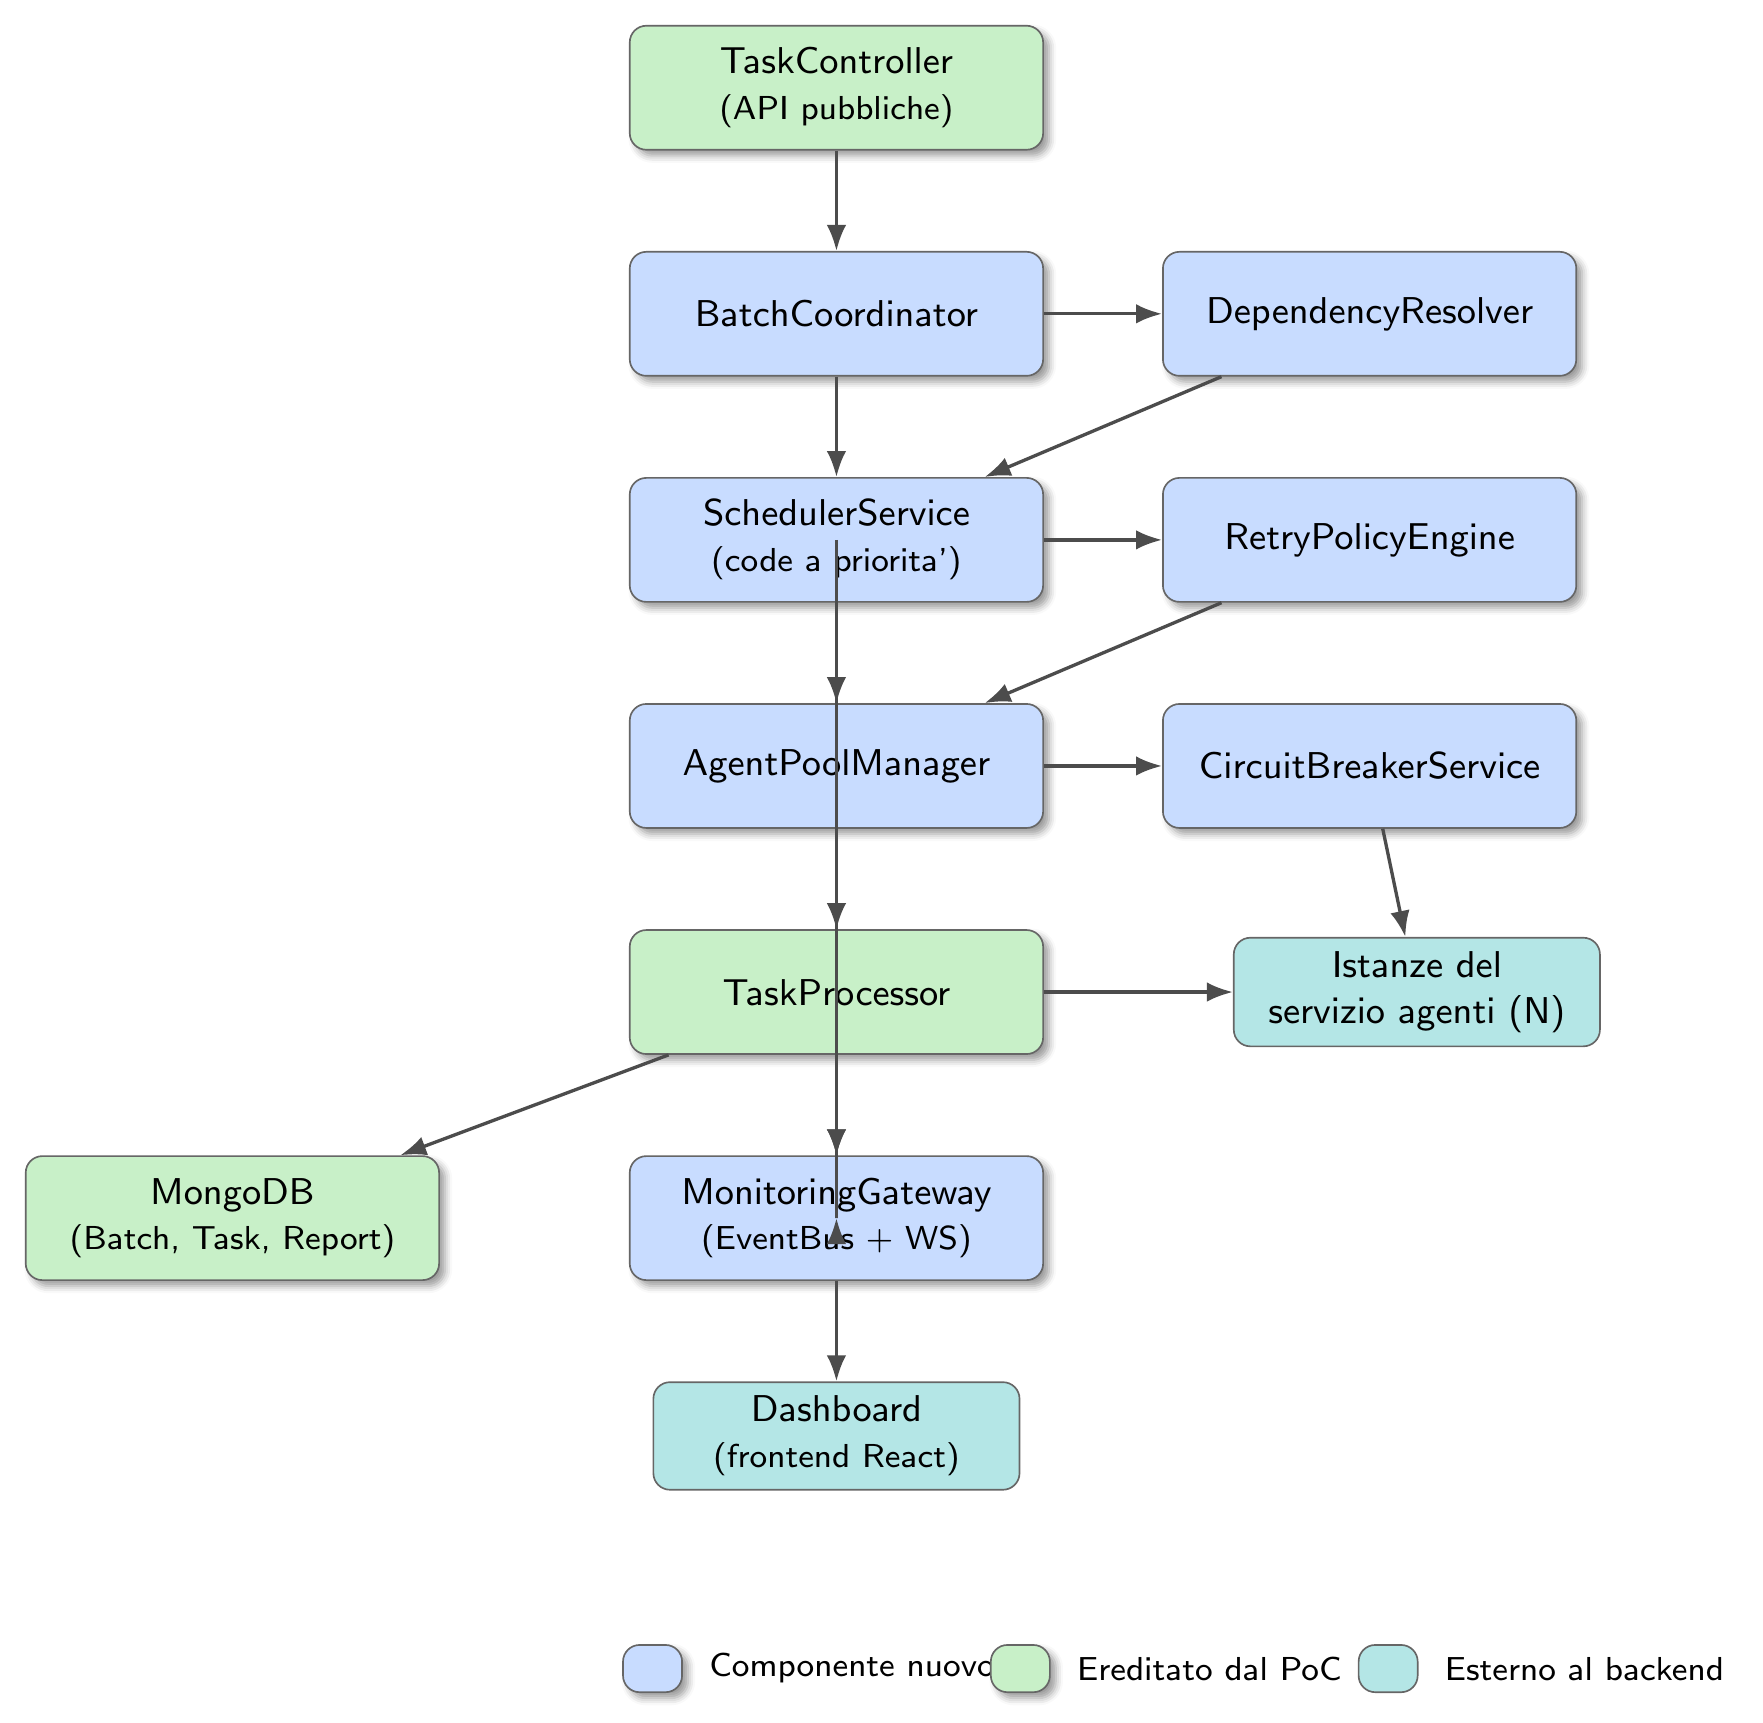
\includegraphics[width=0.62\textwidth]{figures/orchestratore-produzione-componenti.png}
\caption[Architettura dei componenti dell'orchestratore di produzione]{Architettura dei componenti dell'orchestratore di produzione. In blu i componenti nuovi; in verde quelli ereditati dal PoC (adattati); in azzurro gli elementi esterni al backend.}
\label{fig:orch-componenti}
\end{figure}

Il flusso è lineare: \texttt{BatchCoordinator} riceve la definizione del batch dal frontend e la traduce in \texttt{BatchStep} persistiti; \texttt{DependencyResolver} calcola, a ogni transizione di stato, quali passi sono \emph{pronti} (tutte le dipendenze soddisfatte); \texttt{SchedulerService} li accoda rispettando le priorità; \texttt{RetryPolicyEngine} decide, quando un passo fallisce, se e quando riprovarlo; \texttt{AgentPoolManager} sceglie un'istanza sana del servizio agenti e vi inoltra l'esecuzione tramite \texttt{TaskProcessor}, passando per \texttt{CircuitBreakerService} che può rifiutare la chiamata a priori se il bersaglio (LLM o GitHub) è in stato aperto. Ogni componente emette eventi verso \texttt{MonitoringGateway}, che li inoltra alla dashboard via WebSocket e ne persiste un riassunto per le metriche storiche.

\subsection{Modello di dominio esteso}

Il modello del PoC (figura~\ref{fig:domain-model}) si estende con cinque entità nuove, senza modificare \texttt{Report} né la forma esterna di \texttt{Task} (si aggiungono solo campi opzionali retro-compatibili).

\begin{lstlisting}[caption={Entita' nuove del modello di dominio dell'orchestratore.}, label={lst:orch-dominio}]
// Un batch e' ora un grafo, non piu' un insieme piatto di operazioni
interface Batch {
  id: string
  userId: string
  contextId: string
  status: 'DRAFT' | 'SCHEDULED' | 'RUNNING'
         | 'COMPLETED' | 'PARTIALLY_FAILED' | 'FAILED' | 'CANCELLED'
  priority: number              // usata da SchedulerService, default 0
  createdAt: Date
  finishedAt?: Date
}

// Un nodo del DAG: una singola operazione dentro un batch
interface BatchStep {
  id: string
  batchId: string
  operation: OperationCode
  dependsOn: string[]           // id di altri BatchStep dello stesso batch
  status: 'PENDING' | 'READY' | 'RUNNING'
        | 'COMPLETED' | 'FAILED' | 'SKIPPED' | 'CANCELLED'
  taskId?: string                // valorizzato quando lo step viene eseguito
  onFailure: 'BLOCK_DESCENDANTS' | 'SKIP_DESCENDANTS'  // RF.111
}

// Estensione non distruttiva del Task esistente (Sez. 4.3, modello di dominio)
interface Task {
  // ... campi invariati (id, userId, batchId, contextId, operation,
  //     status, progressPercent, currentStage, reportId, error, finishedAt)
  batchStepId?: string          // nullo per le task fuori da un batch DAG
  retryCount: number            // default 0
  retryPolicyId?: string
}

interface RetryPolicy {
  id: string
  operation: OperationCode | '*'   // '*' = policy di default
  maxAttempts: number               // include il primo tentativo
  backoffStrategy: 'EXPONENTIAL' | 'FIXED'
  baseDelayMs: number
  maxDelayMs: number
  retryableErrorKinds: ('TIMEOUT' | 'UPSTREAM')[]  // mai 'PARSING' esaurito
}

interface AgentInstance {
  id: string
  baseUrl: string                 // es. http://agents-2:8000
  status: 'HEALTHY' | 'DEGRADED' | 'DOWN'
  activeTasks: number
  lastHeartbeatAt: Date
}

interface CircuitBreakerState {
  target: 'LLM_PROVIDER' | 'GITHUB_API'
  state: 'CLOSED' | 'OPEN' | 'HALF_OPEN'
  failureCount: number
  openedAt?: Date
}
\end{lstlisting}

Il campo \texttt{onFailure} su \texttt{BatchStep} rende esplicita, per ogni passo, la scelta tra due semantiche legittime quando un suo predecessore fallisce: \texttt{BLOCK\_DESCENDANTS} lascia i discendenti in \texttt{PENDING} indefinitamente (il batch resta \texttt{PARTIALLY\_FAILED} finché un umano non decide), \texttt{SKIP\_DESCENDANTS} li marca \texttt{SKIPPED} e lascia proseguire il resto del DAG. Il default proposto è \texttt{SKIP\_DESCENDANTS}, coerente con l'isolamento dei fallimenti già adottato per i batch piatti del PoC (RF.48): un batch parzialmente riuscito resta più utile di un batch bloccato.

\subsection{Decisioni architetturali dell'orchestratore di produzione (ADR-5 -- ADR-8)}
\label{sub:orch-adr}

Queste quattro decisioni completano le ADR-1--ADR-4 del PoC (\S~\ref{sec:adr}) e riguardano esclusivamente il componente appena descritto; non sono vincolanti per l'MVP (\S~\ref{sec:orchestratore-produzione}, Nota di perimetro), ma lo diventano nel momento in cui l'orchestratore di produzione viene pianificato.

\paragraph{ADR-5 --- Il DAG è persistito come lista di adiacenza in MongoDB, non delegato a un motore esterno.} Un motore di workflow dedicato (Temporal, Camunda) risolverebbe elegantemente retry, timeout e stato distribuito, ma introdurrebbe una dipendenza tecnologica nuova non presente nel capitolato e un secondo sistema di persistenza dello stato da tenere sincronizzato con MongoDB. \textbf{Decisione}: \texttt{BatchStep} come collezione MongoDB con riferimenti \texttt{dependsOn}, risolta lato applicativo da \texttt{DependencyResolver} a ogni transizione di stato. \textbf{Da non fare}: introdurre un motore di workflow esterno finché la complessità dei DAG reali (profondità, fan-out) non lo giustifica; è un'evoluzione possibile, non un prerequisito.

\paragraph{ADR-6 --- Il retry è responsabilità del backend NestJS, non del servizio agenti Python.} Il servizio agenti già implementa una propria autocorrezione a grana fine per gli errori di parsing (fino a due tentativi dentro il grafo LangGraph); estendere quella logica al retry di un intero fallimento \texttt{TIMEOUT}/\texttt{UPSTREAM} frammenterebbe la fonte di verità sullo stato della Task tra due servizi. \textbf{Decisione}: il servizio agenti resta stateless rispetto ai retry; ogni tentativo è un'invocazione nuova e indipendente decisa da \texttt{RetryPolicyEngine} nel backend, che è anche l'unico scrittore dello stato \texttt{Task}. \textbf{Da non fare}: far ritentare al servizio agenti le proprie chiamate al provider LLM oltre l'autocorrezione di parsing già presente, per non duplicare la policy in due posti.

\paragraph{ADR-7 --- Il circuit breaker è per bersaglio condiviso, non per utente o per Task.} LLM e GitHub sono risorse a quota globale: se il circuito restasse per singolo utente, un utente rumoroso potrebbe esaurire la quota mentre il sistema continua a segnalare tutti gli altri circuiti come chiusi, ritentando invano. \textbf{Decisione}: uno stato di circuito per \texttt{LLM\_PROVIDER} e uno per \texttt{GITHUB\_API}, condivisi da tutte le Task di tutti gli utenti. \textbf{Da non fare}: dimensionare le soglie di apertura sul traffico di un singolo utente; vanno tarate sul throughput aggregato atteso.

\paragraph{ADR-8 --- Nessuna affinità tra Task e istanza agente.} Legare una Task all'istanza che l'ha iniziata (per riprendere un tool-calling interrotto, ad esempio) semplificherebbe alcuni casi di ripresa, ma impedirebbe lo scaling orizzontale reale: un'istanza sovraccarica resterebbe tale per le sue Task già assegnate anche se altre istanze sono libere. \textbf{Decisione}: ogni tentativo (primo avvio o retry) può andare a qualunque istanza \texttt{HEALTHY}; lo stato che deve sopravvivere a un cambio di istanza (contesto caricato, cronologia dei messaggi) resta interno all'esecuzione del grafo LangGraph di un singolo tentativo, mai persistito lato Python tra un tentativo e l'altro. \textbf{Da non fare}: introdurre sticky session tra frontend e istanza agente; la sessione utile è quella verso il backend (WebSocket autenticato), non verso il servizio agenti.

\subsection{Ciclo di vita del Batch}

La figura~\ref{fig:orch-batch-lifecycle} mostra gli stati di \texttt{Batch}. A differenza della Task (che ha un ciclo di vita lineare, figura~\ref{fig:stati}), il Batch ha due esiti intermedi possibili (\texttt{COMPLETED} solo se \emph{tutti} i passi sono completati, \texttt{PARTIALLY\_FAILED} se almeno uno è fallito ma altri sono comunque riusciti) oltre al fallimento totale.

\begin{figure}[H]
\centering
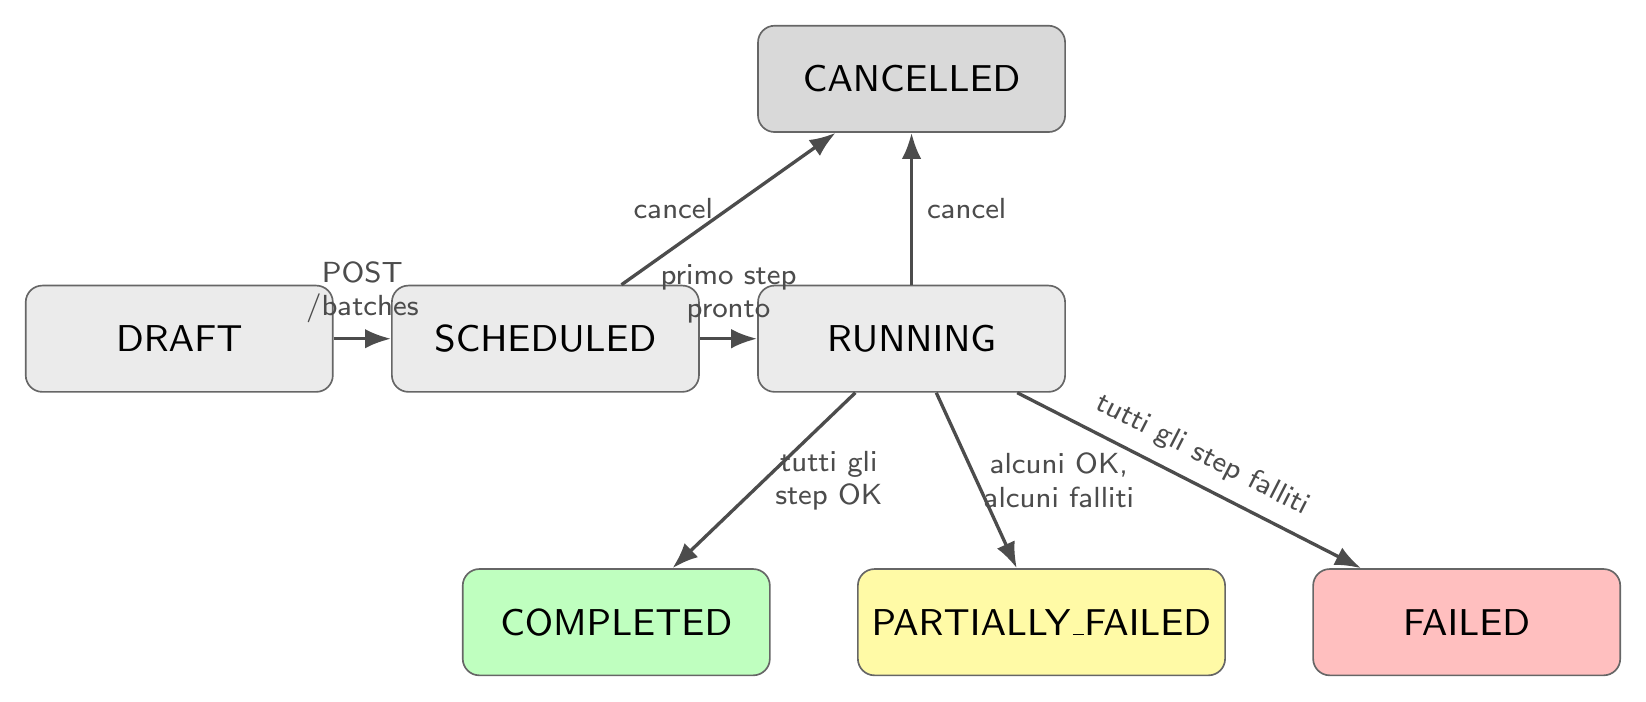
\includegraphics[width=0.85\textwidth]{figures/orchestratore-produzione-stati-batch.png}
\caption[Ciclo di vita di un Batch]{Ciclo di vita di un Batch (RF.106, RF.111). Gli stati terminali (verde/giallo/rosso/grigio) non hanno uscite, come per Task (figura~\ref{fig:stati}).}
\label{fig:orch-batch-lifecycle}
\end{figure}

Un \texttt{BatchStep} attraversa uno stato aggiuntivo rispetto a \texttt{Task}: \texttt{READY}, che rappresenta l'istante in cui \texttt{DependencyResolver} ha verificato che tutte le sue dipendenze sono \texttt{COMPLETED} ma \texttt{SchedulerService} non lo ha ancora estratto dalla coda. La distinzione tra \texttt{READY} e \texttt{RUNNING} è ciò che rende misurabile RQ.12 (l'overhead di scheduling è il tempo trascorso in \texttt{READY}).

\subsection{Retry e circuit breaker}

\texttt{RetryPolicyEngine} interviene in un solo punto: quando \texttt{TaskProcessor} riceve un \texttt{Report} con \texttt{status=FAILED}. Non tutti i fallimenti sono uguali (RS.6): un errore \texttt{PARSING} persistente (il modello non produce mai un JSON valido) non migliora ripetendo la stessa chiamata, mentre un \texttt{TIMEOUT} o un errore \texttt{UPSTREAM} (5xx dal provider, connessione GitHub caduta) spesso sì. Per questo la policy limita il retry automatico ai soli \texttt{error.kind} elencati in \texttt{retryableErrorKinds} --- di default \texttt{TIMEOUT} e \texttt{UPSTREAM}, mai \texttt{PARSING} (che nel servizio agenti ha già un suo meccanismo di autocorrezione a grana più fine, interno al grafo LangGraph, prima ancora di arrivare come \texttt{Report} fallito).

Il ritardo tra un tentativo e il successivo segue un backoff esponenziale con \emph{jitter}, per evitare che più Task fallite nello stesso istante ripartano tutte insieme e ricreino il picco di carico che le aveva fatte fallire:
$$\text{delay}_n = \min(\text{maxDelayMs},\ \text{baseDelayMs} \times 2^{n}) + \text{jitter}(0, \text{baseDelayMs})$$
dove $n$ è il numero del tentativo (0-indicizzato). Ogni retry crea una \emph{nuova} esecuzione della stessa Task (stesso \texttt{id}, incrementando \texttt{retryCount}), non una nuova Task: questo mantiene coerente la relazione uno-a-uno tra Task e la sua storia nel BatchStep, mentre il \texttt{Report} fallito dei tentativi precedenti resta comunque persistito per motivi di audit (l'AccessLog verso GitHub, \S~\ref{sec:github}, resta corretto anche quando un tentativo fallito ha già letto dei file).

Il circuit breaker è per bersaglio (\texttt{LLM\_PROVIDER} o \texttt{GITHUB\_API}), non per singola Task: entrambi sono risorse condivise --- una quota API, un rate limit GitHub --- e un errore a cascata su una li riguarda indipendentemente da quale Task lo ha causato. Segue il pattern standard a tre stati: \texttt{CLOSED} (funzionamento normale) $\to$ \texttt{OPEN} dopo $k$ fallimenti consecutivi entro una finestra temporale (rifiuta le nuove chiamate immediatamente, senza nemmeno tentarle, e le mette in coda per un nuovo giro di retry) $\to$ \texttt{HALF\_OPEN} dopo un periodo di raffreddamento (lascia passare una singola chiamata di prova) $\to$ \texttt{CLOSED} se ha successo o di nuovo \texttt{OPEN} se fallisce. Aprire il circuito verso GitHub non blocca le Task che non hanno tool GitHub attivi (Docs e Changelog, se il loro \texttt{ContextLoader} ha già completato la lettura); aprire il circuito verso il provider LLM blocca invece qualunque Task, perché tutti e tre gli agenti dipendono da \texttt{LLMProvider}.

\subsection{Scaling: il pool di agenti}

Nel PoC il servizio agenti è una singola istanza raggiunta a un indirizzo fisso (\texttt{http://agents:8000}, \S~\ref{sec:scheletro-condiviso}). In produzione questo non basta: se un'istanza è occupata su una scansione Security da 180\,s, le Task in coda aspettano anche se altre istanze sono libere. \texttt{AgentPoolManager} sostituisce l'indirizzo fisso con un registro dinamico di istanze, popolato dalla piattaforma di orchestrazione dei container (repliche Docker Compose in sviluppo, repliche ECS/Fargate in produzione, coerentemente con il target AWS già fissato in \S~\ref{sec:tecnologie}) tramite service discovery, e applica tre meccanismi:

\begin{itemize}
    \item \textbf{Health check}: ogni istanza espone \texttt{GET /health}; \texttt{AgentPoolManager} la interroga ogni 10\,s con timeout 3\,s. Tre fallimenti consecutivi portano lo stato a \texttt{DOWN} e la escludono dal bilanciamento finché non torna a rispondere.
    \item \textbf{Bilanciamento a connessioni attive}: tra le istanze \texttt{HEALTHY}, la Task pronta va a quella con \texttt{activeTasks} più basso (least-connections), non a rotazione semplice: gli agenti hanno tempi di esecuzione molto diversi tra loro (90\,s Docs/Changelog contro 180\,s Security), e una rotazione cieca finirebbe per accumulare lavoro sulle istanze più lente.
    \item \textbf{Nessuna affinità}: ogni Task può essere eseguita da qualunque istanza (ADR-8, sotto), perché lo stato che conta --- Task, Report, AccessLog --- vive nel backend, non nel processo Python. Questo è ciò che rende lo scaling orizzontale possibile senza cambiare il servizio agenti: un'istanza in più è solo un altro consumatore identico della stessa coda.
\end{itemize}

Quando tutte le istanze sono sature o \texttt{DOWN}, le Task pronte restano in coda su BullMQ (nessuna Task viene persa o eseguita in autonomia dal backend): è la stessa garanzia di back-pressure già presente nel PoC (ADR-3), estesa a più consumatori.

\subsection{Dashboard di monitoraggio}

La dashboard (RF.109) è una nuova pagina del frontend React esistente, non un servizio separato: riusa la stessa connessione WebSocket già autenticata (\S~\ref{sub:ws}), sottoscrivendo in più i canali emessi da \texttt{MonitoringGateway}. Mostra quattro riquadri:

\begin{enumerate}
    \item \textbf{Batch attivi}: lista dei batch \texttt{RUNNING} con il loro DAG visualizzato come grafo (nodo verde = \texttt{COMPLETED}, blu = \texttt{RUNNING}, grigio = \texttt{PENDING}/\texttt{READY}, rosso = \texttt{FAILED}, tratteggiato = \texttt{SKIPPED}).
    \item \textbf{Code}: profondità della coda per priorità, età della Task più vecchia in attesa (indicatore diretto di RQ.12 in degrado).
    \item \textbf{Pool di agenti}: stato di ogni \texttt{AgentInstance} (salute, task attive, ultimo heartbeat).
    \item \textbf{Circuit breaker}: stato corrente per \texttt{LLM\_PROVIDER} e \texttt{GITHUB\_API}, con il conteggio dei fallimenti nella finestra corrente.
\end{enumerate}

\begin{table}[H]
\centering
\caption{Nuovi eventi WebSocket emessi da \texttt{MonitoringGateway}, in aggiunta ai quattro già presenti nel PoC (tabella~\ref{tab:ws}).}
\label{tab:orch-eventi-ws}
\vspace{2mm}
\renewcommand{\arraystretch}{1.3}
\begin{tabularx}{\textwidth}{|l|X|}
\hline
\textbf{Evento WS} & \textbf{Payload} \\ \hline
\texttt{batch.step.updated} & \{ batchId, stepId, status, taskId? \} \\ \hline
\texttt{batch.updated} & \{ batchId, status \} \\ \hline
\texttt{agent.health.changed} & \{ instanceId, status, activeTasks \} \\ \hline
\texttt{circuitbreaker.changed} & \{ target, state, failureCount \} \\ \hline
\texttt{queue.depth.updated} & \{ priority, depth, oldestWaitMs \} \\ \hline
\end{tabularx}
\end{table}

\subsection{Contratto API esteso}

Gli endpoint REST pubblici del PoC (\S~\ref{sec:api}) restano validi; l'orchestratore ne aggiunge di nuovi, mantenendo lo stesso prefisso \texttt{/api/v1} e la stessa autenticazione JWT.

\begin{table}[H]
\centering
\caption{Endpoint REST pubblici aggiunti dall'orchestratore.}
\label{tab:orch-endpoint}
\vspace{2mm}
\renewcommand{\arraystretch}{1.3}
\begin{tabularx}{\textwidth}{|l|X|}
\hline
\textbf{Metodo e path} & \textbf{Scopo} \\ \hline
\texttt{POST /batches} & Crea un Batch a partire da una definizione di DAG (\texttt{BatchStep[]} con le rispettive \texttt{dependsOn}); ritorna \texttt{202} + \texttt{\{batchId\}}. \\ \hline
\texttt{GET /batches} & Elenco dei batch dell'utente, con stato aggregato. \\ \hline
\texttt{GET /batches/:id} & Dettaglio di un batch, incluso lo stato di ogni \texttt{BatchStep}. \\ \hline
\texttt{POST /batches/:id/cancel} & Annulla un batch (cancella gli step \texttt{PENDING}/\texttt{READY}, richiede annullamento cooperativo per quelli \texttt{RUNNING}, come già fatto per la singola Task). \\ \hline
\texttt{GET /metrics/summary} & Metriche aggregate: throughput, tasso di successo per operazione, tempo medio di esecuzione. Uso interno/dashboard. \\ \hline
\texttt{GET /agents/pool/status} & Stato corrente del pool di istanze agenti (sola lettura, per la dashboard). \\ \hline
\texttt{GET /circuit-breakers} & Stato corrente dei circuit breaker per bersaglio (sola lettura, per la dashboard). \\ \hline
\end{tabularx}
\end{table}

Gli endpoint interni si estendono di uno solo: \texttt{POST /internal/agents/heartbeat}, che ogni istanza del servizio agenti chiama periodicamente per registrarsi nel pool --- alternativa più semplice alla service discovery quando l'orchestrazione dei container non la offre nativamente (ad esempio in Docker Compose puro).

\subsection{Migrazione dal PoC}

La migrazione è pensata per essere incrementale e non richiedere una riscrittura: ogni passo aggiunge un componente sopra quelli esistenti, mantenendo il sistema funzionante a ogni tappa.

\begin{enumerate}
    \item \textbf{DAG piatto retro-compatibile}: si introduce \texttt{BatchCoordinator} e \texttt{DependencyResolver}, ma ogni batch creato dal frontend attuale (un insieme di operazioni senza dipendenze, come oggi) genera un DAG con zero archi --- ogni \texttt{BatchStep} è già \texttt{READY} dal primo istante. Il comportamento osservabile non cambia finché il frontend non inizia a dichiarare dipendenze esplicite.
    \item \textbf{Retry sopra il TaskProcessor esistente}: si inserisce \texttt{RetryPolicyEngine} nel punto in cui \texttt{TaskProcessor} già gestisce un \texttt{Report} con \texttt{status=FAILED} (\S~\ref{sec:orchestratore}): invece di segnare la Task immediatamente come \texttt{FAILED}, si consulta la policy e si ri-accoda se applicabile. Nessuna modifica al servizio agenti.
    \item \textbf{Pool dinamico}: si sostituisce l'URL statico verso il servizio agenti con \texttt{AgentPoolManager}, inizialmente con una sola istanza registrata (comportamento identico al PoC), poi con repliche multiple quando il capacity planning (RQ.13) lo richiede.
    \item \textbf{Circuit breaker e dashboard}: ultimo livello, perché richiede che i primi tre siano stabili --- non ha senso mostrare in dashboard uno stato di retry o di pool che non esiste ancora.
\end{enumerate}

Nessuno di questi passi tocca il contratto \texttt{Report} né gli endpoint pubblici già consumati dal frontend (\S~\ref{sec:api}): l'orchestratore è un'evoluzione del \emph{come} le Task vengono eseguite, non del \emph{cosa} il frontend riceve.

\subsection{Pattern architetturali aggiuntivi raccomandati}
\label{sub:orch-pattern-aggiuntivi}

I pattern già adottati nel PoC e nell'orchestratore di produzione (facade in \S~\ref{sec:github}, strategy/adapter su \texttt{LLMProvider} e sui \texttt{ContextLoader} per agente, coda con backpressure in ADR-3, circuit breaker per bersaglio in ADR-7, retry con backoff esponenziale e jitter in \S~\ref{sub:orch-adr}, artefatto immutabile in ADR-4) coprono bene la resilienza dell'esecuzione. Restano alcuni punti ciechi, individuati rileggendo il documento nel suo complesso, che non richiedono nuovi servizi AWS né nuove tecnologie: sono estensioni dei componenti già disegnati. Vengono proposti qui come parte della stessa roadmap post-MVP di \S~\ref{sec:orchestratore-produzione}, non come requisiti dell'MVP corrente.

\begin{center}
\footnotesize
\renewcommand{\arraystretch}{1.25}
\begin{xltabular}{\textwidth}{|l|X|X|}
\caption{Pattern architetturali aggiuntivi proposti, con il problema che chiudono e dove si innestano nel disegno esistente.}
\label{tab:orch-pattern-aggiuntivi} \\
\hline
\textbf{Pattern} & \textbf{Problema che chiude} & \textbf{Dove si innesta} \\ \hline
\endfirsthead
\multicolumn{3}{l}{\normalsize\itshape Tabella~\ref{tab:orch-pattern-aggiuntivi} (segue dalla pagina precedente)} \\
\hline
\textbf{Pattern} & \textbf{Problema che chiude} & \textbf{Dove si innesta} \\ \hline
\endhead
\hline
\multicolumn{3}{r}{\normalsize\itshape (continua)} \\
\endfoot
\hline
\endlastfoot
Idempotency Key &
La Parte Frontend segnala come rischio accettato l'assenza di retry automatici client-side (Tabella~\ref{tab:fe-compromessi}): un doppio invio manuale dopo un timeout di rete può creare due batch identici. Un header \texttt{Idempotency-Key} generato dal client, con indice univoco lato \texttt{Batch}/\texttt{Task} per una finestra di deduplica, chiude il buco senza introdurre retry automatici. &
\texttt{POST /tasks} (\S~\ref{sec:api}) e \texttt{POST /batches} (Tabella~\ref{tab:orch-endpoint}). \\ \hline
Outbox Pattern &
Lo stato \texttt{Task} è scritto su MongoDB e l'evento è emesso via WebSocket/BullMQ come due operazioni distinte: se il processo cade tra le due, l'evento si perde e il polling di riallineamento (\S~\ref{sub:ws}) resta l'unica rete di sicurezza. Un outbox transazionale (l'evento scritto nella stessa transazione Mongo dello stato, drenato da un publisher separato) elimina la classe di bug ``evento perso silenziosamente''. &
\texttt{TaskProcessor} e \texttt{MonitoringGateway} (\S~\ref{sec:orchestratore-produzione}, Architettura dei componenti). \\ \hline
Bulkhead &
\texttt{AgentPoolManager} bilancia a connessioni attive su un pool omogeneo, ma Security (timeout 180\,s) e Docs/Changelog (90\,s) hanno profili di esecuzione molto diversi: una raffica di scansioni OWASP può occupare tutte le istanze anche con bilanciamento a least-connections. Isolare code/capacità per famiglia di operazione evita che un agente ne affami un altro. &
Scaling: il pool di agenti (\S~\ref{sec:orchestratore-produzione}). \\ \hline
Dead Letter Queue &
Una Task che esaurisce \texttt{maxAttempts} in \texttt{RetryPolicyEngine} oggi diventa semplicemente \texttt{FAILED}: nessun posto dedicato la rende ispezionabile in massa dal team operativo, che deve altrimenti filtrare lo storico report a mano. &
Retry e circuit breaker (\S~\ref{sub:orch-adr}); si aggancia a RF.109 (dashboard). \\ \hline
Optimistic Concurrency Control &
Con \texttt{Desired Count: 1} il rischio è nullo, ma nel momento in cui anche il backend NestJS (non solo il pool agenti) scala orizzontalmente, due istanze potrebbero contendersi la stessa transizione di stato su \texttt{Task}/\texttt{BatchStep}. Un campo di versione (o un compare-and-swap sullo status atteso) previene la corsa critica prima che serva. &
Modello di dominio esteso (\S~\ref{sec:orchestratore-produzione}): campi \texttt{Task} e \texttt{BatchStep}. \\ \hline
Feature Flag &
La Tabella~\ref{tab:fe-compromessi} prevede già un fallback ``stub'' per l'input interattivo del Changelog in caso di taglio budget (RF.98--RF.102): oggi sarebbe un ramo di codice da ricompilare e ridistribuire. Un booleano letto da Parameter Store rende il fallback un toggle operativo invece di un nuovo deploy --- utile proprio nello scenario di emergenza per cui è previsto. &
Segreti e Configurazione (\S~\ref{sec:aws-config}), variabile aggiuntiva accanto a quelle di Tabella~\ref{tab:aws-env}. \\ \hline
Secret Rotation &
\texttt{JWT\_SECRET}, \texttt{CREDENTIAL\_MASTER\_KEY} e \texttt{INTERNAL\_SHARED\_SECRET} sono creati una volta in Secrets Manager (\S~\ref{sec:aws-checklist}) ma nessuna politica ne prevede la rotazione periodica: un gap tipico in sede di audit di sicurezza. &
Segreti e Chiavi (\S~\ref{sec:aws-checklist}) e Segreti e Configurazione (\S~\ref{sec:aws-config}). \\ \hline
\end{xltabular}
\end{center}

Nessuno di questi sette punti richiede una nuova ADR vincolante per l'MVP: sono annotati qui come debito tecnico consapevole, da valutare insieme al proponente quando si pianifica l'evoluzione oltre il perimetro descritto nella Parte~\ref{part:frontend-spec} e nella Parte~\ref{part:aws-manuale}.

\section{Sintesi e prossimi passi}
\label{sec:sintesi}

Il PoC dimostra molto più di ``un agente funziona'': prova che i tre agenti condividono backbone, provider e contratto di output, differendo solo in due punti localizzati, e prova che l'intero stack applicativo (backend NestJS/MongoDB, frontend React, servizio agenti Python) si integra con quel core e con GitHub in modo end-to-end. È un'affermazione architetturale più forte di quella delle stesure precedenti, e copre la soglia di integrazione richiesta dal proponente. Resta un PoC: una operazione per agente, orchestrazione minima, gli stessi rami d'errore per tutti, nessuna scrittura verso l'esterno e infrastruttura locale in attesa della migrazione ad AWS.

I passi immediatamente successivi, una volta condiviso questo perimetro, sono: la stesura dei template di prompt (Docs, OWASP, Changelog) che i profili caricheranno; la scelta e la validazione del fornitore LLM sul golden set; l'implementazione della facade GitHub con la sua whitelist e i tre tool; e la preparazione dei componenti di interfaccia condivisi per la visualizzazione del \texttt{Report}. Il passo successivo, quando l'orchestrazione minima (\S~\ref{sec:orchestratore}) non basterà più, è l'evoluzione verso l'orchestratore di produzione progettato in \S~\ref{sec:orchestratore-produzione}: batch come DAG, retry automatico, scaling del pool di agenti e dashboard di monitoraggio, migrabile in modo incrementale senza toccare il contratto \texttt{Report} né gli endpoint già consumati dal frontend.

Questi passi sono stati effettivamente percorsi. Le due Parti che seguono documentano il risultato: la Parte~\ref{part:frontend-spec}--\ref{part:frontend-adr} progetta il frontend dell'MVP (autenticazione, ruoli, credenziali, storico, esportazione PDF) riusando lo stack e i contratti validati qui; la Parte~\ref{part:aws-manuale}--\ref{part:aws-adr} progetta l'infrastruttura AWS di produzione (VPC, ECS su Fargate, MongoDB Atlas, Bedrock) che sostituisce Docker Compose senza toccare il codice applicativo. Insieme, le tre parti raccontano l'intero percorso dal PoC all'MVP.

\part{Frontend MVP --- Specifica Operativa (UX/UI)}
\label{part:frontend-spec}

\emph{Questa parte contiene esclusivamente le specifiche implementative, la mappa delle pagine, i flussi operativi e le regole di visibilità del frontend. I principi guida, le motivazioni delle scelte e le decisioni architetturali (ADR-FE) sono documentati nella Parte~\ref{part:frontend-adr}.}

\section{Perimetro del documento}
\label{sec:fe-perimetro}

\subsection{Obiettivo}

Il presente documento definisce la progettazione UX/UI del frontend di \textbf{Code Guardian} per la release MVP, a partire dai requisiti descritti nell'Analisi dei Requisiti (AdR). L'architettura e lo stack tecnologico validati nel Proof of Concept (Parte~\ref{part:poc}) vengono riutilizzati come base implementativa; le funzionalità non coperte in quella fase (autenticazione, storico, esportazione PDF) vengono qui progettate ex novo. Tutte le scelte operative rispettano i vincoli definiti nella Parte~\ref{part:aws-manuale} (Progettazione Infrastruttura AWS).

\subsection{Cosa progetto}
\label{sec:fe-cosa-progetto}

\begin{itemize}
    \item L'intero flusso di autenticazione e la gestione del ruolo operativo dell'utente (\textbf{Sviluppatore}, \textbf{Security Auditor}, \textbf{Project Manager}), definito in fase di registrazione.
    \item La configurazione delle credenziali dei servizi esterni (GitHub e Task Management unificati).
    \item La selezione del contesto operativo (repository, riferimento di base, ambito di analisi).
    \item La configurazione, l'avvio e il monitoraggio delle operazioni degli agenti tramite canale realtime.
    \item La visualizzazione del report strutturato, estesa con il collegamento alla Pull Request generata dal backend e l'esportazione in formato PDF.
    \item Lo storico dei report pregressi.
    \item Le regole di visibilità e abilitazione delle interfacce in base al ruolo dell'utente autenticato.
\end{itemize}

\subsection{Cosa non progetto (fuori perimetro MVP)}

I seguenti requisiti sono esclusi dal perimetro della presente progettazione:

\begin{itemize}
    \item \textbf{RF.18} --- Selezione di una Pull Request come riferimento di base (UC9.2, UC9.5, UC14). Il tipo di riferimento supportato è esclusivamente \emph{Branch} (con hash di Commit opzionale).
    \item \textbf{RF.38, RF.75--RF.78} --- Impostazioni di notifica e flussi di invio email (UC21.2, UC30--UC33).
    \item \textbf{RF.79--RF.81} --- Gestione e personalizzazione del template del README (UC34, UC34.1--UC34.3). L'Agente Docs opera esclusivamente con il template di default.
\end{itemize}

\subsection{Mappatura Componenti PoC $\to$ Frontend MVP}

La Tabella~\ref{tab:fe-mappatura-componenti} mappa le aree funzionali validate nel Proof of Concept rispetto alle azioni implementative previste per il frontend dell'MVP.

\begin{table}[H]
\centering
\caption{Mappatura dei componenti del PoC riutilizzati, estesi o introdotti ex novo per il frontend dell'MVP.}
\label{tab:fe-mappatura-componenti}
\vspace{2mm}
\renewcommand{\arraystretch}{1.2}
\begin{tabularx}{\textwidth}{|X|l|X|}
\hline
\textbf{Area validata nel PoC} & \textbf{Riuso} & \textbf{Azione per l'MVP} \\ \hline
Stack (React, Vite, TanStack Router, pnpm, Zustand) & Totale & Nessuna modifica: stack confermato e utilizzato come base di partenza. \\ \hline
\texttt{sessionStore} & Esteso & Conversione da store di sola presenza del token a store di sessione autenticata (aggiunta utente, JWT, ruolo attivo e stato credenziali). \\ \hline
\texttt{selectionStore} & Totale & Nessuna modifica strutturale: rimozione dell'opzione Pull Request dal tipo di riferimento. \\ \hline
\texttt{tasksStore} + Client WebSocket & Esteso & Integrazione della gestione degli stati interattivi (UC41.1, UC43) per le richieste di input utente. Questo flusso costituisce un'estensione reale rispetto al PoC e richiede l'introduzione di un nuovo evento WS e di un nuovo endpoint REST. \\ \hline
Configurazione Token (GitHub) & Esteso & Evoluzione in schermata generica di ``Servizi connessi'', per supportare estensioni future. \\ \hline
Pagina \texttt{/select} & Totale & Riuso dell'albero di selezione contestuale; rimosso il ramo Pull Request. \\ \hline
Pagina \texttt{/run} & Esteso & Aggiunta logica di disabilitazione e filtraggio delle operazioni in base al ruolo attivo. \\ \hline
Pagina \texttt{/tasks} (Dashboard) & Esteso & Supporto alla renderizzazione condizionale per gli stati interattivi (inserimento Sprint ID, conferma metadati). \\ \hline
Rendering del Report & Esteso & Mantenuto il dispatcher a blocchi polimorfi. Il componente \texttt{Proposal} viene esteso promuovendo a elemento primario il link alla Pull Request. \\ \hline
Esportazione report & Esteso & Sostituzione dei formati \texttt{.md}/\texttt{.json} con l'invocazione dell'endpoint backend per il download del file \texttt{.pdf}. \\ \hline
Autenticazione e Storico & Nuovo & Componenti e viste progettate ex novo, in quanto non necessarie nella validazione tecnologica del PoC. \\ \hline
\end{tabularx}
\end{table}

\section{Architettura dell'informazione}

\subsection{Ruoli e permessi}

Il sistema prevede tre specializzazioni di Utente Generico: lo \textbf{Sviluppatore}, il \textbf{Security Auditor / Team Lead} e il \textbf{Project Manager}. Il ruolo viene selezionato in fase di registrazione e rimane fisso per l'intera durata dell'account, coerentemente con i requisiti di base del sistema.

Ogni ruolo eredita le funzionalità trasversali (selezione del repository, monitoraggio, visualizzazione ed esportazione dei report) e aggiunge l'accesso privilegiato alle operazioni del proprio dominio, come delineato nella Tabella~\ref{tab:fe-ruoli-operazioni}.

\begin{table}[H]
\centering
\caption{Mappatura delle operazioni per ruolo operativo.}
\label{tab:fe-ruoli-operazioni}
\vspace{2mm}
\renewcommand{\arraystretch}{1.2}
\begin{tabularx}{\textwidth}{|X|X|l|}
\hline
\textbf{Operazione} & \textbf{Attore abilitato} & \textbf{Codice Op.} \\ \hline
Generazione/aggiornamento README & Sviluppatore & \texttt{DOCS\_README} \\ \hline
Documentazione inline (JSDoc) & Sviluppatore & \texttt{DOCS\_INLINE} \\ \hline
Documentazione API & Sviluppatore & \texttt{DOCS\_API} \\ \hline
Scansione vulnerabilità OWASP Top 10 & Security Auditor / Team Lead & \texttt{SECURITY\_OWASP} \\ \hline
Verifica conformità Policy-as-code & Security Auditor / Team Lead & \texttt{SECURITY\_POLICY} \\ \hline
Changelog tecnico & Project Manager / Sviluppatore & \texttt{CHANGELOG\_TECHNICAL} \\ \hline
Changelog di business & Project Manager & \texttt{CHANGELOG\_BUSINESS} \\ \hline
\end{tabularx}
\end{table}

\textbf{Regola di visibilità (Filtraggio):} La lista delle operazioni disponibili sulla pagina di avvio mostra \emph{esclusivamente} le opzioni abilitate per il ruolo attivo dell'utente. Le operazioni non permesse vengono omesse dall'interfaccia (nessuna visualizzazione in stato disabilitato). Questo filtraggio è applicato nativamente dall'endpoint backend in base al ruolo dichiarato nel token di sessione.

\subsection{Mappa delle pagine e delle rotte}

L'accesso alle pagine è regolato dallo stato di autenticazione e dallo stato della credenziale GitHub. La Figura~\ref{fig:fe-navmap} illustra la mappa di navigazione principale e i reindirizzamenti (redirect) condizionali applicati dalle guardie di rotta (dettagliate in \S~\ref{sec:fe-guardie}).

\begin{figure}[H]
\centering
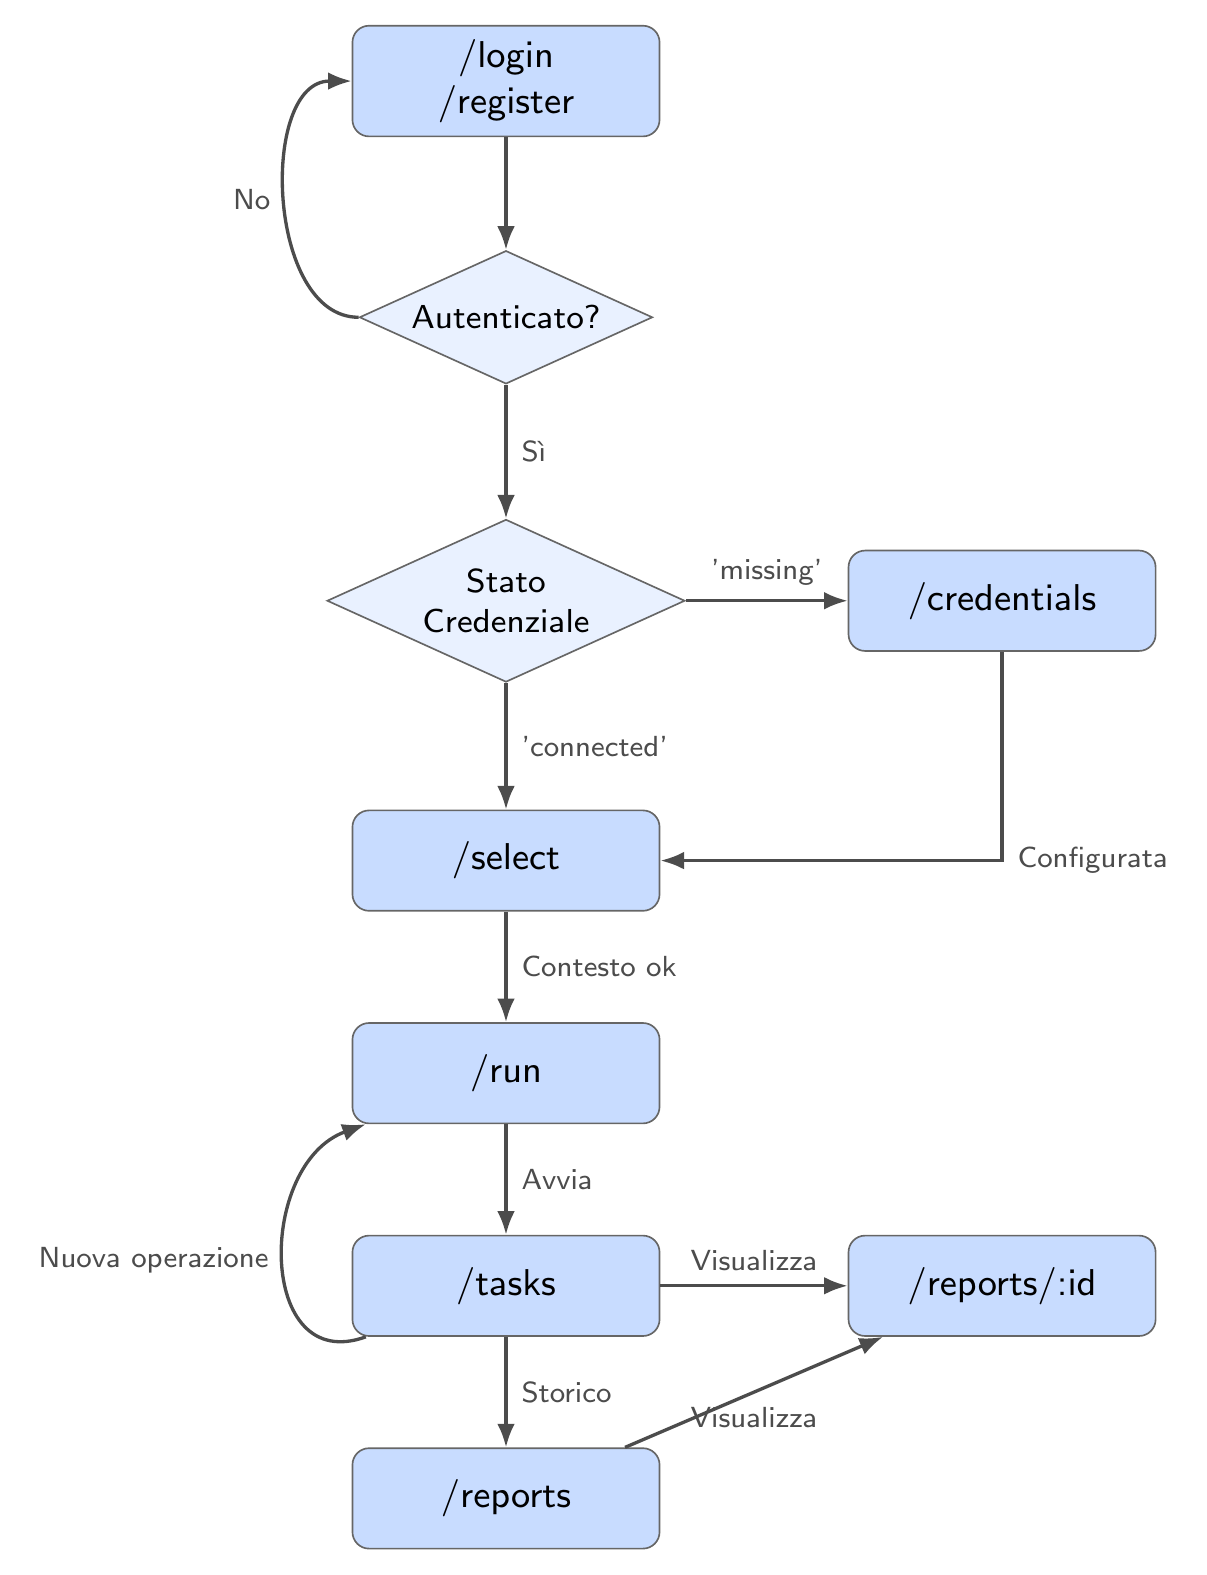
\includegraphics[width=0.6\textwidth]{figures/fe-navmap.png}
\caption[Mappa di navigazione principale e reindirizzamenti condizionali del frontend]{Mappa di navigazione principale e reindirizzamenti condizionali del frontend.}
\label{fig:fe-navmap}
\end{figure}

La Tabella~\ref{tab:fe-rotte} definisce le rotte dell'applicazione, i ruoli ammessi e gli endpoint REST consumati da ciascuna di esse.

\begin{table}[H]
\centering
\caption{Mappa delle rotte del frontend e relative dipendenze API.}
\label{tab:fe-rotte}
\vspace{2mm}
\renewcommand{\arraystretch}{1.2}
\begin{tabularx}{\textwidth}{|l|l|l|X|}
\hline
\textbf{Pagina} & \textbf{Rotta} & \textbf{Ruoli} & \textbf{Endpoint consumati} \\ \hline
Registrazione & \texttt{/register} & Non autenticato & \texttt{POST /auth/register} \\ \hline
Login & \texttt{/login} & Non autenticato & \texttt{POST /auth/login} \\ \hline
Servizi connessi & \texttt{/credentials} & Tutti & \texttt{POST /credentials}, \texttt{.../validate}, \texttt{GET /credentials} \\ \hline
Selezione contesto & \texttt{/select} & Tutti & \texttt{GET /repositories}, \texttt{.../refs}, \texttt{.../tree}, \texttt{POST /contexts} \\ \hline
Avvio operazioni & \texttt{/run} & Tutti (filtrate) & \texttt{GET /operations}, \texttt{POST /tasks} \\ \hline
Dashboard & \texttt{/tasks} & Tutti & \texttt{GET /tasks}, \texttt{POST /tasks/:id/cancel}, \texttt{POST /tasks/:id/input}, WebSocket \\ \hline
Storico report & \texttt{/reports} & Tutti & \texttt{GET /reports} \\ \hline
Dettaglio report & \texttt{/reports/:id} & Tutti & \texttt{GET /reports/:id}, \texttt{GET /reports/:id/export?format=pdf} \\ \hline
\end{tabularx}
\end{table}

\subsection{Credenziali e servizi esterni}

La schermata \texttt{/credentials} è implementata come una lista scalabile di \texttt{ServiceCredential}. Nell'MVP è presente un unico servizio esterno configurabile: \textbf{GitHub}. Questo singolo token assolve a entrambe le necessità descritte nei requisiti (accesso al codice e accesso al sistema di Task Management/Issue).

\textbf{Invalidazione a runtime:} Se durante l'esecuzione di un'operazione il backend rileva che il token GitHub non è più valido (es. scadenza o revoca), l'operazione in corso fallisce con codice \texttt{CREDENTIAL\_INVALID}. Il frontend intercetta questo stato tramite l'evento WebSocket, aggiorna lo stato globale dell'utente a \texttt{'invalid'} e mostra un banner persistente che invita a riconfigurare la credenziale su \texttt{/credentials}, bloccando nel frattempo l'avvio di nuove analisi.

\section{Flussi utente per ruolo}

\subsection{Notazione}

I flussi sono descritti come sequenze ordinate di schermate, per mantenere la tracciabilità rispetto agli scenari principali dell'Analisi dei Requisiti. I punti di diramazione per errore (validazioni fallite, timeout, superamento soglie) non sono ripetuti qui, poiché seguono tutti il pattern di stato interrotto descritto in \S~\ref{sec:fe-errori}.

\subsection{Flusso trasversale: accesso e configurazione iniziale}

Comune a tutti e tre i ruoli, precede qualunque operazione degli agenti.

\begin{enumerate}
    \item L'utente non autenticato arriva su \texttt{/login}. Se non possiede un account, passa a \texttt{/register}, compila l'anagrafica, le credenziali e seleziona il proprio ruolo operativo iniziale.
    \item Al primo login, l'utente privo di credenziali configurate viene reindirizzato a \texttt{/credentials}: nessuna operazione degli agenti è raggiungibile senza almeno un servizio connesso e validato.
    \item L'utente inserisce il token GitHub; il sistema esegue la validazione sintattica locale e la chiamata di test prima di persistere la credenziale.
    \item Completata la configurazione, l'utente accede a \texttt{/select} per definire il contesto operativo: URL del repository, branch e, opzionalmente, hash del commit e ambito di analisi.
    \item Il contesto salvato (\texttt{contextId}) è condiviso da tutte le operazioni successive avviate nella stessa sessione di lavoro; l'utente procede a \texttt{/run}.
\end{enumerate}

Le credenziali e il contesto restano validi tra una sessione e l'altra: un utente già configurato, ai login successivi, salta direttamente da \texttt{/login} a \texttt{/run} o a \texttt{/select} se desidera cambiare repository.

\subsection{Selezione ed avvio multiplo delle operazioni (trasversale)}

Questo flusso è indipendente dal ruolo attivo, il quale determina unicamente le operazioni visibili sulla schermata.

\begin{enumerate}
    \item Su \texttt{/run} il sistema recupera ed elenca le operazioni disponibili per il ruolo attivo dell'utente.
    \item L'utente seleziona/deseleziona una o più operazioni (selezione multipla supportata).
    \item L'utente conferma l'avvio. Il sistema verifica lato client la presenza di almeno un'operazione selezionata e dei prerequisiti di contesto raccolti in \S~3.2.
    \item Il sistema invia \texttt{POST /tasks} con l'elenco delle operazioni e reindirizza l'utente a \texttt{/tasks}, dove ciascuna operazione avviata compare come elemento indipendente della dashboard, partendo dallo stato di \emph{In attesa} (\texttt{PENDING}).
    \item Ogni operazione procede in isolamento, delegando al backend la gestione della concorrenza (le operazioni per lo stesso agente rimarranno \emph{In attesa} finché l'orchestrazione non le sbloccherà). Il fallimento di un'analisi non blocca o invalida le altre.
\end{enumerate}

\subsection{Flusso Sviluppatore --- Agente Docs}

Copre le operazioni di Generazione README, Documentazione inline e Documentazione API. Condividono lo stesso flusso a livello di interfaccia.

\begin{enumerate}
    \item Lo Sviluppatore segue il flusso comune (\S~3.2, \S~3.3), selezionando una o più operazioni del dominio Docs.
    \item Su \texttt{/tasks}, l'operazione avanza attraverso gli stati \emph{In attesa} $\to$ \emph{In elaborazione} $\to$ \emph{Completato}, senza ulteriori input richiesti.
    \item Al completamento, lo Sviluppatore apre il report. Il corpo del report mostra come elemento primario il collegamento alla Pull Request aperta automaticamente dal backend; per la documentazione inline, include inoltre gli avvisi di complessità eccessiva come elementi a gravità informativa.
    \item Lo Sviluppatore valuta la proposta direttamente su GitHub: l'interfaccia non prevede un passo di approvazione interno.
\end{enumerate}

\subsection{Flusso Security Auditor / Team Lead --- Agente Security}

Copre la Scansione vulnerabilità OWASP e la Verifica conformità Policy-as-code.

\begin{enumerate}
    \item Il Security Auditor / Team Lead segue il flusso comune, selezionando le operazioni di sicurezza.
    \item Per la verifica policy-as-code, nessun input aggiuntivo è richiesto (la presenza del file \texttt{POLICY.md} è validata automaticamente dal backend).
    \item Al completamento, il report mostra l'elenco dei riscontri come lista strutturata filtrabile per gravità: per ciascun elemento vengono esposti categoria, gravità, riferimento al file/riga e la \emph{remediation} proposta tramite snippet di codice o testo descrittivo.
\end{enumerate}

\subsection{Flusso Project Manager --- Agente Changelog}

È il flusso con la maggiore interattività, in quanto prevede punti di sospensione a metà esecuzione per l'inserimento e la validazione di input da parte dell'utente. La Figura~\ref{fig:fe-changelog-seq} illustra lo scambio di eventi e schermate.

Al termine dell'elaborazione, il Project Manager visualizza il changelog tecnico formattato in Markdown con i collegamenti ipertestuali ai ticket di origine.

\subsubsection{Dipendenza di esecuzione tra Changelog tecnico e di business}

Coerentemente con la precondizione di UC41 (``L'utente ha selezionato l'operazione `Generazione changelog tecnico' o `Generazione changelog di business'''), la selezione di \texttt{CHANGELOG\_BUSINESS} in \texttt{/run} è sufficiente e autonoma: non richiede la co-selezione di \texttt{CHANGELOG\_TECHNICAL}. L'Orchestratore avvia un'unica Task con \texttt{operation: 'CHANGELOG\_BUSINESS'} che attraversa due fasi interne allo stesso stato \texttt{RUNNING}:

\begin{enumerate}
    \item Generazione del Changelog tecnico (UC41), il cui esito viene reso disponibile all'utente come report intermedio.
    \item Sospensione dell'esecuzione: la Task valorizza \texttt{pendingInput} con \texttt{kind: 'BUSINESS\_\allowbreak{}CONFIRMATION'}, forzando in Dashboard l'espansione dell'area interattiva con i comandi ``Accetta e genera Business'' / ``Annulla'' (UC45/UC46) --- lo stesso pattern grafico già usato per lo Sprint ID.
    \item Alla conferma, la medesima Task riprende l'elaborazione e genera il Changelog di business (UC45), transitando infine a \texttt{COMPLETED}.
\end{enumerate}

\begin{figure}[H]
\centering
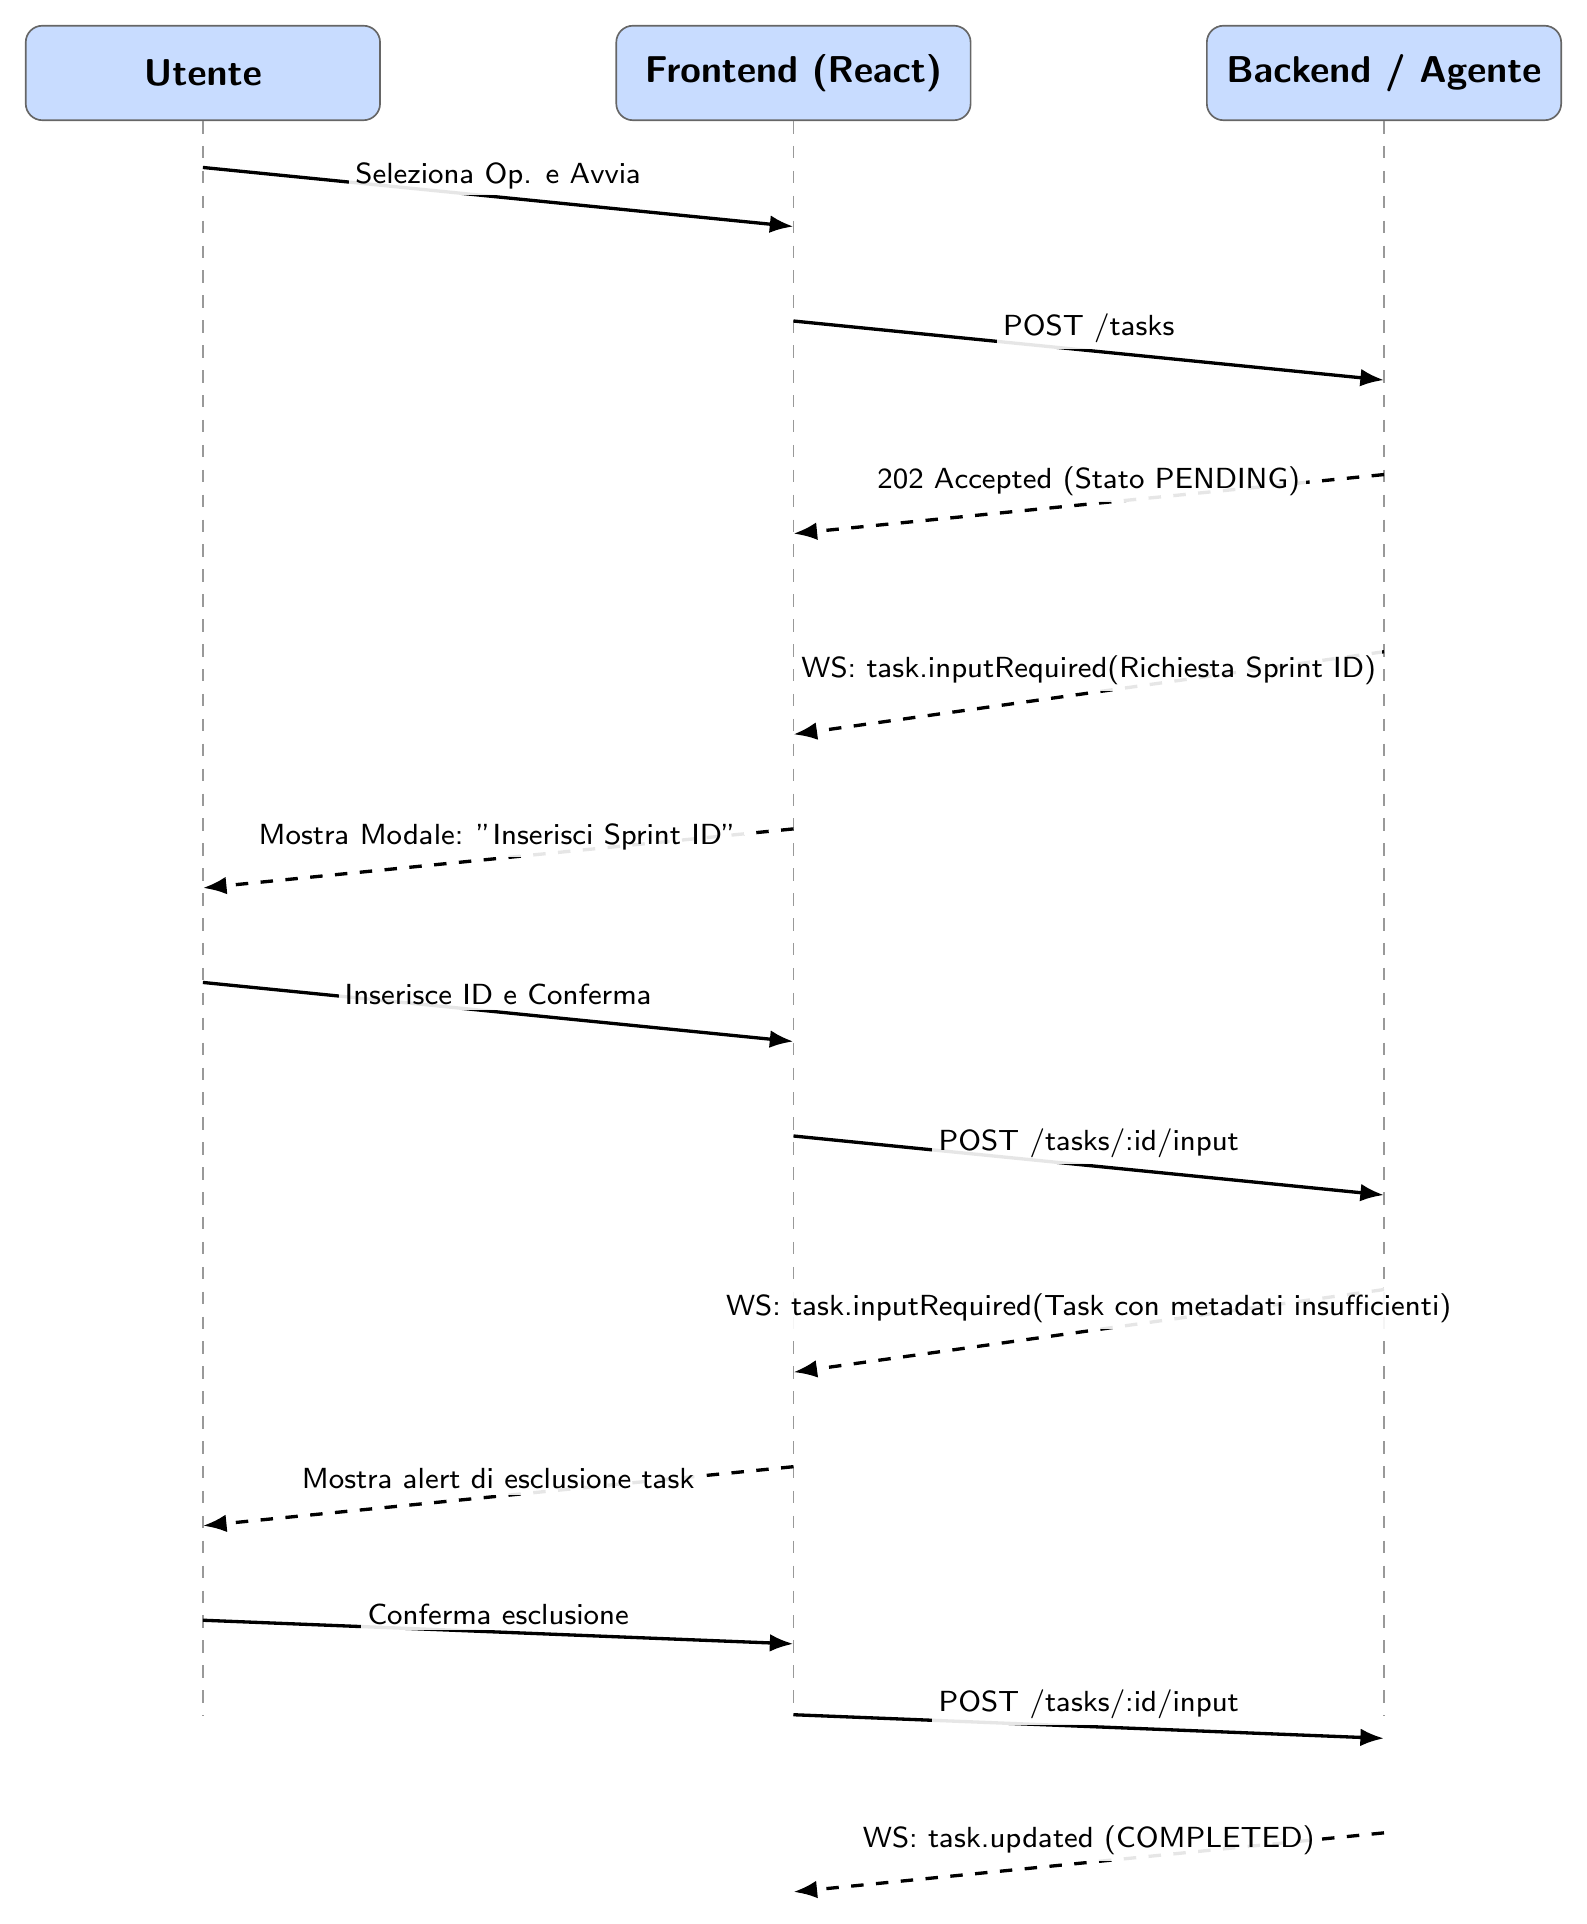
\includegraphics[width=0.85\textwidth]{figures/fe-changelog-seq.png}
\caption[Diagramma di sequenza delle interazioni intermedie per l'Agente Changelog]{Diagramma di sequenza delle interazioni intermedie per l'Agente Changelog.}
\label{fig:fe-changelog-seq}
\end{figure}

In Dashboard, dall'avvio alla conclusione, l'operazione compare quindi come un \textbf{singolo elemento}, non come due Task distinte. Se l'utente desidera anche un report tecnico standalone (senza business), seleziona separatamente \texttt{CHANGELOG\_TECHNICAL}: in tal caso viene creata una seconda Task indipendente, che non ha alcuna relazione con l'eventuale Task \texttt{CHANGELOG\_BUSINESS} avviata in parallelo (nessuna Task condivide risultati con l'altra; ciascuna esegue la propria generazione tecnica in isolamento).

\begin{quote}
\textbf{Nota Implementativa.} La scelta di mantenere disaccoppiati i comandi di selezione in UI e delegare l'attesa all'Orchestratore backend evita di inserire rigida logica di business all'interno del client. Il frontend si limita a leggere lo stato \texttt{pendingInput} inoltrato tramite WebSocket e a renderizzare le modali di conseguenza, ignorando del tutto le motivazioni sequenziali che lo hanno innescato.
\end{quote}

\subsection{Flusso trasversale: consultazione dei report pregressi}

\begin{enumerate}
    \item Da qualunque punto dell'applicazione, l'utente autenticato raggiunge \texttt{/reports}, che elenca i report salvati con identificativo, titolo, data e ora di generazione.
    \item La selezione di un elemento apre \texttt{/reports/:id}. La pagina di dettaglio del report è un unico componente condiviso, raggiungibile sia dalla dashboard (a operazione appena completata) sia dallo storico.
    \item Da entrambi i punti di ingresso, l'utente può richiedere l'esportazione in PDF, generato lato backend e reso disponibile in download.
\end{enumerate}

\subsection{Flusso trasversale: rilevamento di una credenziale non più valida}

Questo evento può interrompere qualunque flusso in qualsiasi momento.

\begin{enumerate}
    \item Durante l'esecuzione di un'operazione, il backend incontra un errore 401/403 nel leggere dal servizio esterno.
    \item Il backend marca la Task come \texttt{FAILED} con codice \texttt{CREDENTIAL\_INVALID}; l'evento WebSocket trasporta questa informazione.
    \item Il frontend aggiorna la Task interessata come un normale fallimento e imposta lo stato della credenziale globale a \texttt{'invalid'} (\S~2.3).
    \item L'intestazione applicativa mostra un banner persistente su tutte le pagine finché lo stato resta \texttt{'invalid'}, offrendo un collegamento diretto a \texttt{/credentials}.
    \item Ripristinata la connessione, il banner scompare e le guardie di rotta (\S~\ref{sec:fe-guardie}) tornano a consentire l'accesso pieno alle operazioni.
\end{enumerate}

\section{Wireframe descrittivi delle schermate}

\subsection{Notazione}

Ogni schermata è descritta per regioni di layout (intestazione, corpo, aree laterali o modali) e per elementi ordinati dall'alto verso il basso. I riferimenti tra parentesi (UC/RF) individuano il requisito di origine; i riferimenti preceduti da \texttt{Componente:} rimandano al catalogo del Design System (\S~5.3), in cui l'elemento è definito e stilizzato una singola volta.

\subsection{Registrazione --- \texttt{/register}}

\textbf{Corpo.} Modulo centrato a colonna singola:
\begin{itemize}
    \item Campo testo \textbf{Nome} (UC1.1, RF.2).
    \item Campo testo \textbf{Cognome} (UC1.1, RF.2).
    \item Campo testo \textbf{Indirizzo email} (UC1.3, RF.3), con validazione inline al cambio del focus.
    \item Campo \textbf{Password} (UC1.4, RF.3).
    \item \textbf{Selettore di ruolo} (UC1.5, RF.4) a scelta singola (Sviluppatore, Security Auditor / Team Lead, Project Manager) con riga di descrizione sintetica per opzione.
    \item Pulsante di conferma primario ``Crea account''.
    \item Collegamento secondario verso \texttt{/login} per l'utente già registrato.
\end{itemize}

\textbf{Stati.}
\begin{itemize}
    \item \emph{Email già registrata} (UC2/RF.5): messaggio non bloccante sopra il modulo, con link diretto a \texttt{/login}.
    \item \emph{Dati non validi} (UC3/RF.6): \texttt{Componente: Campo di modulo con validazione inline}. Il pulsante primario resta disabilitato.
\end{itemize}

\subsection{Login --- \texttt{/login}}

\textbf{Corpo.} Modulo centrato:
\begin{itemize}
    \item Campo testo \textbf{Indirizzo email} (UC4.1, RF.8).
    \item Campo \textbf{Password} (UC4.2, RF.8).
    \item Pulsante di conferma primario ``Accedi''.
    \item Collegamento secondario verso \texttt{/register}.
\end{itemize}

\textbf{Stati.}
\begin{itemize}
    \item \emph{Credenziali errate} (UC5/RF.9): messaggio d'errore generico posizionato sopra il modulo, senza indicare quale campo specifico è errato.
    \item \emph{Successo}: redirect condizionale a \texttt{/credentials} (se token assente) o \texttt{/select} (se token presente e valido).
\end{itemize}

\subsection{Servizi connessi --- \texttt{/credentials}}

\textbf{Corpo.} Lista generica di provider (nell'MVP, un solo elemento).
\begin{itemize}
    \item Elemento ``GitHub'' con sottotitolo esplicativo. Come argomentato in \S~2.3, questo singolo campo collassa e assolve contestualmente all'inserimento del token per l'accesso al codice (RF.11) e per l'accesso al sistema di Task Management (RF.12).
    \item \emph{Se non configurato}: campo di input per il token e pulsante ``Connetti''.
    \item \emph{Se configurato}: etichetta di stato ``Connesso'' con timestamp, pulsanti ``Verifica di nuovo'' e ``Rimuovi''.
    \item Area informativa inferiore sulla predisposizione per futuri provider.
\end{itemize}

\textbf{Stati.}
\begin{itemize}
    \item \emph{Formato non valido} (UC8/RF.14): errore inline sul campo prima dell'invio.
    \item \emph{Validazione fallita} (UC7/RF.13): messaggio d'errore del servizio. Pulsante ``Continua'' disabilitato.
    \item \emph{Credenziale invalidata a runtime} (\S~2.3): messaggio dedicato ``Il token risulta scaduto o revocato'', stesso comportamento dello stato di validazione fallita.
\end{itemize}

\subsection{Selezione del contesto --- \texttt{/select}}

\textbf{Corpo, prima area (Repository e riferimento).}
\begin{itemize}
    \item Campo testo \textbf{URL del repository Git} (UC9.1, RF.16).
    \item Campo testo \textbf{Nome del branch} (UC9.3, RF.17), con autocompletamento attivo post-validazione URL (UC11/RF.20).
    \item Campo testo opzionale \textbf{Hash del commit} (UC9.4, RF.17).
\end{itemize}

\textbf{Corpo, seconda area (Ambito di analisi, abilitata post-validazione).}
\begin{itemize}
    \item \texttt{Componente: Albero file} per la selezione a tre stati (file/directory). Selezionare una directory marca ricorsivamente i figli (UC16.2, RF.28).
    \item Comando rapido ``Seleziona intero repository'' (UC16.1, RF.26).
    \item Contatore in tempo reale (file e righe stimate) con soglia visiva (UC19/RF.31).
    \item Pulsante di conferma primario ``Conferma contesto''.
\end{itemize}

\textbf{Stati.}
\begin{itemize}
    \item \emph{Repository o riferimento non trovati/permessi mancanti}: errore inline sul campo.
    \item \emph{Linguaggio non supportato}: avviso non bloccante sopra l'albero (UC15/RF.24).
    \item \emph{Ambito vuoto/inaccessibile}: messaggio d'errore bloccante prima dell'invio (UC17, UC18).
\end{itemize}

\subsection{Avvio operazioni --- \texttt{/run}}

\textbf{Corpo.}
\begin{itemize}
    \item Lista delle operazioni disponibili, già filtrata in base al ruolo utente (\S~2.1). Ogni operazione della Tabella~\ref{tab:fe-ruoli-operazioni} --- incluso \texttt{CHANGELOG\_BUSINESS} --- compare come voce indipendente e paritetica, coerentemente con UC20.1/UC21.1.
    \item Per ogni operazione: Nome, descrizione sintetica, casella di selezione.
    \item \texttt{CHANGELOG\_BUSINESS} è selezionabile e avviabile autonomamente, senza necessità di selezionare anche \texttt{CHANGELOG\_TECHNICAL}: la generazione tecnica è inclusa come primo passo interno della stessa Task (\S~3.6.1).
    \item Pulsante di conferma primario ``Avvia''.
\end{itemize}

\textbf{Stati.}
\begin{itemize}
    \item \emph{Nessuna operazione selezionata}: impedimento all'attivazione del pulsante (UC21.4/RF.41).
\end{itemize}

\subsection{Dashboard --- \texttt{/tasks}}

\textbf{Corpo.} Lista delle operazioni del batch corrente (UC22).
\begin{itemize}
    \item Nome dell'operazione.
    \item \texttt{Componente: Indicatore di stato} (\emph{In attesa}, \emph{In elaborazione}, \emph{Completato}, \emph{Fallito}, \emph{Annullato}) e barra di avanzamento (RF.46).
    \item Comando ``Annulla'' (attivo in \emph{attesa}/\emph{elaborazione}).
    \item Comando ``Visualizza report'' (attivo in \emph{Completato} o \emph{Fallito}).
\end{itemize}

\textbf{Aree interattive (Agente Changelog).} Espansioni \emph{inline} per le task in stato di richiesta input:
\begin{itemize}
    \item \emph{Richiesta Sprint ID} (UC41.1): campo testo, comandi ``Conferma/Annulla'' (UC42).
    \item \emph{Metadati insufficienti} (UC43): elenco identificativi scartabili, comandi ``Procedi escludendo/Annulla operazione'' (UC44).
    \item \emph{Conferma Changelog di business} (\texttt{pendingInput.kind === 'BUSINESS\_CONFIRMATION'}): anteprima del changelog tecnico appena generato, comandi ``Accetta e genera Business'' (UC45) / ``Annulla'' (UC46).
\end{itemize}

L'elemento della Dashboard associato a un'operazione \texttt{CHANGELOG\_BUSINESS} resta un unico elemento per l'intera durata del flusso (generazione tecnica, attesa conferma, generazione business): non vengono mai mostrate due righe distinte per la stessa selezione.

\textbf{Stati.}
\begin{itemize}
    \item \emph{Errore di orchestrazione}: \texttt{Componente: Stato d'errore} limitato al singolo elemento fallito, garantendo l'isolamento visivo (UC23/RF.48).
\end{itemize}

\subsection{Dettaglio report --- \texttt{/reports/:id}}

\textbf{Intestazione.} Riga di metadati: repository, riferimento, ambito analizzato, tempo di esecuzione, timestamp (UC26.1).

\textbf{Corpo (Dispatcher a blocchi).} Ordine e tipo definiti dalla risposta API:
\begin{itemize}
    \item \texttt{TextBlock}: Markdown renderizzato (changelog).
    \item \texttt{FindingBlock} / \texttt{PolicyViolationBlock}: Liste strutturate filtrabili per gravità (Agente Security) con \texttt{Componente: Snippet di codice} per le remediation.
    \item \texttt{Proposal}: \texttt{Componente: Collegamento Pull Request} (elemento primario) e anteprima diff collassabile (Agente Docs).
    \item \texttt{Modulo di validazione}: Comandi di accettazione/annullamento (changelog di business).
\end{itemize}

\textbf{Comandi di pagina.}
\begin{itemize}
    \item Pulsante ``Esporta PDF'' (UC28/RF.73) con indicatore di caricamento.
\end{itemize}

\textbf{Stati.}
\begin{itemize}
    \item \emph{Status FAILED}: Corpo sostituito dal \texttt{Componente: Stato d'errore} (tipo, fase, messaggio).
    \item \emph{Esportazione fallita}: Errore transitorio a pagina (UC29).
\end{itemize}

\subsection{Storico report --- \texttt{/reports}}

\textbf{Corpo.}
\begin{itemize}
    \item Lista di elementi report (UC24): identificativo, titolo descrittivo, timestamp.
    \item Selezione elemento $\to$ navigazione verso \texttt{/reports/:id} (UC25).
\end{itemize}

\subsection{Intestazione applicativa}

Elemento persistente su tutte le rotte autenticate.
\begin{itemize}
    \item Nome dell'utente autenticato.
    \item \texttt{Componente: Indicatore di stato} utilizzato come badge di sola lettura per il ruolo assegnato.
    \item \textbf{Banner di credenziale invalidata} (\S~2.3): fascia d'avviso non bloccante per la navigazione in lettura, con collegamento a \texttt{/credentials}.
    \item Comando ``Esci''.
\end{itemize}

\textbf{Stati.}
\begin{itemize}
    \item \emph{Fallimento di rete (Logout)}: Errore contestuale al tentativo di uscita.
\end{itemize}

\section{Design System e componenti condivisi}

\subsection{Stack di implementazione}

Il design system dell'MVP è implementato utilizzando \textbf{Tailwind CSS} come base per le classi di utilità (\emph{utility-first}) e \textbf{shadcn/ui} come libreria di primitive accessibili per i componenti interattivi complessi (modali, selettori, form). Questa scelta tecnologica garantisce nativamente il rispetto del requisito \textbf{RV.5}, assicurando la piena compatibilità senza anomalie grafiche sulle versioni più recenti dei principali browser desktop (Google Chrome, Mozilla Firefox, Microsoft Edge v145 o superiore).

\subsection{Token visivi}

I token sono definiti come variabili di tema globali, in modo da poter essere declinati visivamente senza modificare il codice dei singoli componenti che li consumano.

\begin{table}[H]
\centering
\caption{Categorie di token visivi condivisi e ambito di applicazione.}
\label{tab:fe-token}
\vspace{2mm}
\renewcommand{\arraystretch}{1.2}
\begin{tabularx}{\textwidth}{|l|X|}
\hline
\textbf{Categoria di token} & \textbf{Uso previsto} \\ \hline
Colori semantici di stato & Un colore per ciascuno dei cinque stati operativi (\emph{Attesa, Elaborazione, Completato, Fallito, Annullato}). Riusati identicamente nell'Indicatore di stato e in ogni badge o messaggio che comunica un esito. \\ \hline
Colori semantici di gravità & Un colore per ciascun livello di gravità delle segnalazioni dell'Agente Security (\emph{Critica, Alta, Media, Bassa, Informativa}). Il livello informativo è riusato per gli avvisi di complessità dell'Agente Docs. \\ \hline
Colore di superficie neutra & Sfondo di pagina, delle card e dei moduli; un'unica scala di grigi utilizzata per l'intera applicazione. \\ \hline
Tipografia & Una famiglia font per il testo dell'interfaccia (etichette, corpo, moduli) e una famiglia monospaziata dedicata esclusivamente agli Snippet di codice e ai riferimenti a percorsi/righe di file. \\ \hline
Spaziatura & Scala unica su base 4px, applicata uniformemente per garantire coerenza tra densità informative molto diverse (es. form di login vs lista report Security). \\ \hline
Raggio e ombreggiatura & Valori unici per card, finestre modali e badge, per mantenere la stessa grammatica visiva tra le diverse aree dell'applicativo. \\ \hline
\end{tabularx}
\end{table}

\subsection{Catalogo dei componenti condivisi}

I seguenti componenti sono definiti una sola volta e riusati in tutte le schermate descritte in \S~4.

\begin{itemize}
    \item \textbf{Indicatore di stato:} Etichetta testuale con colore semantico associato, usata nella Dashboard e per lo stato dei servizi connessi. Include opzionalmente una barra di avanzamento.
    \item \textbf{Badge di gravità:} Etichetta compatta con colore semantico, usata per i riscontri di sicurezza e gli avvisi di complessità del codice.
    \item \textbf{Albero file:} Struttura ad albero navigabile con caselle di selezione a tre stati (non selezionato, selezionato, parzialmente selezionato), usata nella selezione dell'ambito di analisi.
    \item \textbf{Blocco di report:} Componente \emph{dispatcher} che, dato un elemento del payload di risposta, renderizza il sottocomponente corretto in base al tipo (testo, lista, snippet, modulo).
    \item \textbf{Collegamento Pull Request:} Pulsante o link in evidenza verso la Pull Request aperta dal backend, con anteprima del \emph{diff} disponibile come dettaglio secondario collassabile.
    \item \textbf{Snippet di codice:} Contenitore monospaziato con evidenziazione sintattica minima, usato per il codice correttivo proposto e per le anteprime diff.
    \item \textbf{Modulo di validazione:} Coppia di comandi (primario/secondario) con testo esplicativo, usato per innescare i changelog di business e per le aree interattive della Dashboard.
    \item \textbf{Stato d'errore:} Componente a pagina intera o a riquadro che riporta il tipo di errore, la fase in cui si è verificato e il messaggio descrittivo (\S~\ref{sec:fe-errori}).
    \item \textbf{Campo di modulo con validazione inline:} Campo di input con stato neutro/errore e messaggio contestuale posizionato al di sotto del campo stesso.
\end{itemize}

\subsection{Stati interattivi comuni}

Ogni componente che avvia una richiesta di rete (REST) espone sempre tre stati distinti, per garantire un feedback visivo immediato:

\begin{enumerate}
    \item \textbf{In corso:} Il controllo che ha originato la richiesta mostra un indicatore di caricamento e viene disabilitato per prevenire invii duplicati.
    \item \textbf{Esito positivo:} Transizione visiva immediata verso lo stato successivo previsto (es. redirect, aggiornamento lista, chiusura modale). L'utente non viene mai lasciato sulla schermata originaria con un semplice messaggio di conferma senza indicazioni.
    \item \textbf{Esito negativo:} Attivazione del componente \texttt{Stato d'errore} o del campo in stato di errore (\S~\ref{sec:fe-errori}), senza perdita dei dati già inseriti dall'utente nella form.
\end{enumerate}

\subsection{Accessibilità (A11y)}

L'utilizzo di \texttt{shadcn/ui} fornisce nativamente la navigazione da tastiera, la corretta attribuzione dei ruoli ARIA e la gestione visibile del focus. Come regola aggiuntiva di progettazione, i colori semantici di stato e gravità (\S~5.2) devono essere sempre accompagnati da un'etichetta testuale esplicita, e non essere mai affidati alla sola percezione cromatica.

\section{Stato applicativo}

\subsection{Principio generale}

L'applicazione adotta una politica rigorosa per la gestione dello stato globale: entra in uno \emph{store} Zustand esclusivamente ciò che deve sopravvivere a un cambio di rotta (pagina) o che deve essere letto contemporaneamente da più componenti distanti nell'albero. Tutto il resto rimane relegato allo stato locale del singolo componente o della singola pagina.

La Figura~\ref{fig:fe-store-arch} illustra l'architettura dei tre store globali dell'applicativo e le loro direttrici di comunicazione.

\begin{figure}[H]
\centering
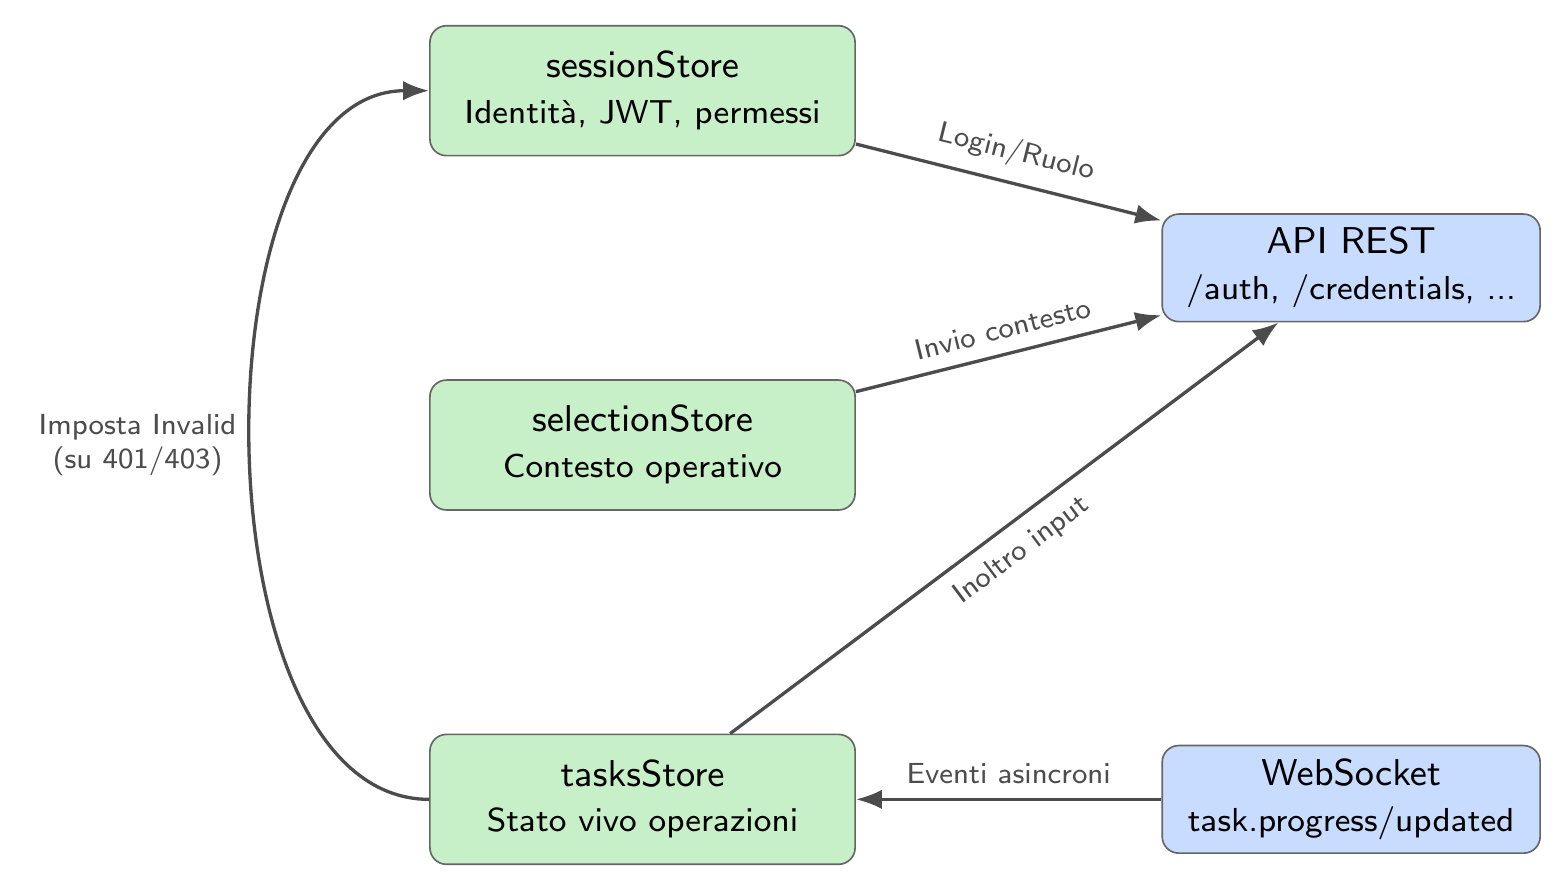
\includegraphics[width=0.85\textwidth]{figures/fe-store-arch.png}
\caption[Architettura degli store applicativi]{Architettura degli store applicativi, comunicazione di rete ed effetti collaterali.}
\label{fig:fe-store-arch}
\end{figure}

\begin{quote}
\textbf{Attenzione.} Il JSON Web Token non deve \textbf{mai} essere salvato all'interno del \texttt{localStorage} o del \texttt{sessionStorage} del browser. Poiché l'MVP non prevede protezioni WAF avanzate contro attacchi XSS, conservare il token esclusivamente nella memoria volatile dello store Zustand garantisce che uno script malevolo non possa estrarlo in modo persistente.
\end{quote}

\subsection{\texttt{sessionStore} --- Identità e credenziali}
\label{sec:fe-sessionstore}

Mantiene la sessione utente e lo stato autorizzativo. Il JSON Web Token (JWT) è mantenuto esclusivamente in memoria (nello store) e mai persistito nel \texttt{localStorage}. Una ricarica completa della pagina richiede un nuovo login.

\begin{lstlisting}[caption={Interfaccia del sessionStore.}]
interface SessionState {
  user: { id: string; firstName: string; role: UserRole } | null
  token: string | null
  credentialsStatus: 'unknown' | 'missing' | 'connected' | 'invalid'
  isAuthenticated: () => boolean

  login(user, token): void
  logout(): void
  setCredentialsStatus(status): void
  markCredentialsInvalid(): void
}

type UserRole = 'DEVELOPER' | 'SECURITY_AUDITOR' | 'PROJECT_MANAGER'
\end{lstlisting}

\begin{itemize}
    \item \textbf{Campo \texttt{role}:} Unica fonte di verità per le regole di visibilità delle operazioni (\S~2.1). Popolato al login e immutabile per la durata della sessione.
    \item \textbf{Campo \texttt{credentialsStatus}:} Evita di interrogare \texttt{GET /credentials} su ogni rotta protetta. Il valore \texttt{'invalid'} differisce da \texttt{'missing'}: indica che una credenziale configurata è stata revocata o è scaduta durante l'utilizzo.
\end{itemize}

\subsection{\texttt{selectionStore} --- Contesto operativo}

Contiene il \texttt{contextId} e i parametri dell'ambito di analisi in uso nella sessione corrente. Viene popolato dalla pagina \texttt{/select} e letto in fase di avvio dalle richieste della pagina \texttt{/run}.

\subsection{\texttt{tasksStore} --- Stato vivo delle operazioni}
\label{sec:fe-tasksstore}

Contiene lo stato in tempo reale delle operazioni correnti, aggiornato asincronamente dagli eventi WebSocket inviati dal backend. La Figura~\ref{fig:fe-task-lifecycle} descrive la macchina a stati di una Task gestita da questo store.

\begin{figure}[H]
\centering
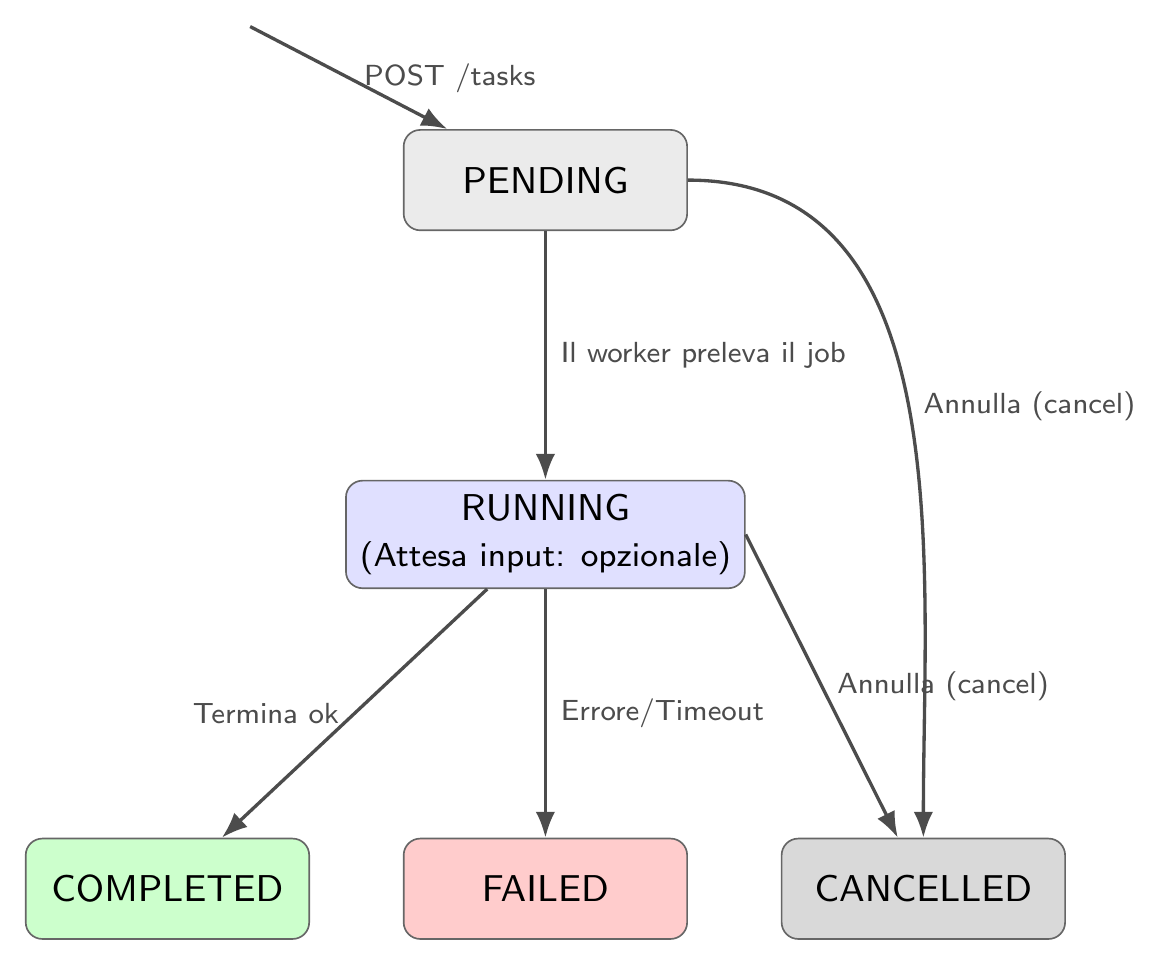
\includegraphics[width=0.85\textwidth]{figures/fe-task-lifecycle.png}
\caption[Ciclo di vita di una Task (frontend)]{Ciclo di vita di una Task. La richiesta di input (\texttt{pendingInput}) non costituisce un nuovo stato, ma una condizione sospensiva interna allo stato \texttt{RUNNING}.}
\label{fig:fe-task-lifecycle}
\end{figure}

Il campo \texttt{pendingInput}, quando valorizzato, è il segnale che innesca l'espansione dell'area interattiva sulla Dashboard (\S~4). L'annullamento della Task, anche durante la fase di input, avviene invocando l'azione unificata \texttt{cancel(taskId)}.

\begin{lstlisting}[caption={Interfaccia del tasksStore con gestione input interattivi.}]
interface TasksState {
  tasks: Record<string, TaskEntry>
  upsertFromEvent(event: TaskEvent): void  // event: task.progress | task.updated
  cancel(taskId): void                     // chiamata a POST /tasks/:id/cancel
  resolvePendingInput(taskId, response): void  // risoluzione input utente
}

interface TaskEntry {
  id: string
  operation: OperationCode
  status: 'PENDING' | 'RUNNING' | 'COMPLETED' | 'FAILED' | 'CANCELLED'
  progressPercent: number
  currentStage: string | null
  reportId: string | null
  error: { code: string; message: string; stage: string } | null

  pendingInput: PendingInput | null
}

type PendingInput =
  | { kind: 'SPRINT_ID' }
  | { kind: 'INCOMPLETE_TASKS'; taskIds: string[] }
  | { kind: 'BUSINESS_CONFIRMATION'; technicalReportId: string }
\end{lstlisting}

\textbf{Effetto collaterale su \texttt{session\allowbreak{}Store}:} Alla ricezione dell'evento \texttt{task.failed} con \texttt{error.code === 'CREDENTIAL\_\allowbreak{}INVALID'}, l'handler del \texttt{tasks\allowbreak{}Store} invoca l'azione \texttt{mark\allowbreak{}Credentials\allowbreak{}Invalid()} del \texttt{session\allowbreak{}Store}. È l'unico punto architetturale in cui uno store modifica lo stato di un altro, in risposta a un evento di rete che invalida le credenziali a livello globale.

\subsection{Dati intenzionalmente non globali}

Per il principio di separazione dichiarato, le seguenti entità rimangono confinate allo stato locale di React (\texttt{useState} o \texttt{useQuery}):

\begin{itemize}
    \item La lista dei servizi connessi (\texttt{GET /credentials}), letta e mostrata unicamente dalla pagina \texttt{/credentials}.
    \item L'albero dei file del repository e l'elenco di \emph{refs}, necessari solo in \texttt{/select}.
    \item La cache dello storico dei report (\texttt{GET /reports}), mantenuta per la sola pagina \texttt{/reports}.
    \item Il contenuto del singolo report aperto (\texttt{GET /reports/:id}).
\end{itemize}

\subsection{Guardie di rotta}
\label{sec:fe-guardie}

Le restrizioni di navigazione client-side si basano unicamente sulla lettura sincrona del \texttt{sessionStore}. Non vengono effettuate chiamate di rete al momento del cambio rotta.

\begin{itemize}
    \item \textbf{Accesso bloccato per utenti autenticati:} \texttt{/login} e \texttt{/register} (redirect a \texttt{/run}).
    \item \textbf{Accesso bloccato per utenti non autenticati:} Tutte le altre rotte (redirect a \texttt{/login}).
    \item \textbf{Accesso in lettura a Task e Report:} Libero per tutti gli utenti autenticati, indipendentemente dallo stato delle credenziali GitHub (inclusi \texttt{'missing'} o \texttt{'invalid'}).
    \item \textbf{Avvio nuove operazioni bloccato:} Se \texttt{credentialsStatus} è \texttt{'missing'} o \texttt{'invalid'}, l'accesso a \texttt{/select} e la conferma di avvio su \texttt{/run} effettuano un redirect immediato a \texttt{/credentials}.
\end{itemize}

\section{Contratto API consumato}
\label{sec:fe-contratto-api}

\subsection{Principi generali del contratto}

Il contratto API si appoggia sul design architetturale già validato nella fase di Proof of Concept (Parte~\ref{part:poc}). Il frontend aderisce ai seguenti vincoli strutturali:

\begin{itemize}
    \item \textbf{Prefisso globale:} Tutte le rotte consumate dal frontend sono esposte sotto il prefisso \texttt{/api/v1}. Le chiamate utilizzano esclusivamente percorsi relativi, delegando l'instradamento all'infrastruttura sottostante (dettagliato in \S~\ref{sec:fe-vincoli-aws}).
    \item \textbf{Separazione dei piani:} Esiste una netta separazione tra il piano pubblico (browser $\to$ backend) e il piano interno (agenti $\to$ backend). Il frontend ha visibilità e accesso unicamente al piano pubblico.
    \item \textbf{Autenticazione realtime:} La connessione al canale WebSocket viene autenticata trasmettendo il JSON Web Token (JWT) durante la fase di \emph{handshake}.
\end{itemize}

\begin{quote}
\textbf{Attenzione --- Vincoli di Rete Ereditati dall'Infrastruttura AWS:}
\begin{itemize}
    \item \textbf{Nessun setup CORS:} Il frontend e il backend sono serviti dalla stessa origine (CloudFront). Non configurare intercettori per preflight OPTIONS, né iniettare header CORS custom nei client HTTP (come Axios o Fetch API).
    \item \textbf{Path Relativi (Vite):} È categoricamente vietato inserire URL assoluti (es. \texttt{https://api...}) all'interno della variabile d'ambiente \texttt{VITE\_API\_BASE\_URL}. Usare sempre percorsi relativi (es. \texttt{/api/v1}). Hardcodare un dominio causerà il fallimento silente delle pipeline CI/CD tra i vari ambienti.
\end{itemize}
\end{quote}

\subsection{Endpoint REST pubblici}

La Tabella~\ref{tab:fe-endpoint} elenca gli endpoint del piano pubblico consumati dal frontend, inclusivi delle estensioni implementate per l'MVP (autenticazione, gestione credenziali, storico, esportazione PDF ed elaborazione input asincroni).

L'endpoint di esportazione report utilizza esclusivamente il formato PDF. La generazione avviene lato backend e il frontend consuma il file direttamente in streaming (nel corpo della risposta HTTP).

\begin{table}[H]
\centering
\caption{Endpoint REST pubblici consumati dal frontend, raggruppati per area funzionale.}
\label{tab:fe-endpoint}
\vspace{2mm}
\renewcommand{\arraystretch}{1.15}
\begin{tabularx}{\textwidth}{|X|X|l|}
\hline
\textbf{Metodo e Path} & \textbf{Scopo} & \textbf{Requisiti} \\ \hline
\multicolumn{3}{|l|}{\textit{Autenticazione}} \\ \hline
\texttt{POST /auth/register} & Registrazione, include il ruolo operativo & RF.1--6 \\ \hline
\texttt{POST /auth/login} & Login, restituisce il JWT & RF.7--9 \\ \hline
\texttt{GET /auth/me} & Profilo e ruolo dell'utente autenticato & RF.7 \\ \hline
\multicolumn{3}{|l|}{\textit{Servizi Connessi}} \\ \hline
\texttt{GET /credentials} & Elenco dei provider configurati e relativo stato & RF.10 \\ \hline
\texttt{POST /credentials} & Salva una credenziale per un provider & RF.10--11 \\ \hline
\texttt{POST /credentials/:id/validate} & Verifica la validità e i permessi del token & RF.13, RS.4 \\ \hline
\texttt{DELETE /credentials/:id} & Rimuove una credenziale & UC6 \\ \hline
\multicolumn{3}{|l|}{\textit{Contesto Operativo}} \\ \hline
\texttt{GET /repositories} & Elenco dei repository accessibili dall'utente & RF.15 \\ \hline
\texttt{GET /repositories/\allowbreak{}:owner/\allowbreak{}:repo/refs} & Branch disponibili & RF.16--17 \\ \hline
\texttt{GET /repositories/\allowbreak{}:owner/\allowbreak{}:repo/tree} & Struttura del repository (richiede \texttt{?ref=}) & RF.25--28 \\ \hline
\texttt{POST /contexts} & Crea l'\texttt{AnalysisContext} & RF.15--31 \\ \hline
\multicolumn{3}{|l|}{\textit{Avvio ed Esecuzione}} \\ \hline
\texttt{GET /operations} & Operazioni disponibili (già filtrate per ruolo) & RF.32--34 \\ \hline
\texttt{POST /tasks} & Avvia una o più task & RF.36--42 \\ \hline
\texttt{GET /tasks} & Elenco delle task per la Dashboard & RF.43--45 \\ \hline
\texttt{GET /tasks/:id} & Dettaglio di una singola task & RF.45--46 \\ \hline
\texttt{POST /tasks/:id/cancel} & Annulla una task, anche durante l'attesa di input & RF.46, UC42, UC44 \\ \hline
\texttt{POST /tasks/:id/input} & Risolve una richiesta di input utente in sospeso (Sprint ID o esclusione task) & UC41.1, UC43, RF.98 \\ \hline
\multicolumn{3}{|l|}{\textit{Storico e Report}} \\ \hline
\texttt{GET /reports} & Storico dei report & RF.49--52 \\ \hline
\texttt{GET /reports/:id} & Dettaglio di un report & RF.53--64 \\ \hline
\texttt{GET /reports/:id/\linebreak[0]export?format=pdf} & Esporta il report in PDF (streaming binario) & RF.73--74 \\ \hline
\end{tabularx}
\end{table}

\subsection{Canale realtime (WebSocket)}

Il canale WebSocket è utilizzato in modalità unidirezionale (backend $\to$ frontend) per il flusso applicativo. Il frontend emette unicamente l'evento di sottoscrizione, mentre le risposte applicative fornite dall'utente non transitano per il socket, bensì tramite l'endpoint REST \texttt{POST /tasks/:id/input}.

In caso di caduta della connessione di rete, alla riapertura del socket il frontend esegue un polling di riallineamento tramite \texttt{GET /tasks} per recuperare l'eventuale stato \texttt{pendingInput} o gli avanzamenti persi.

\begin{quote}
\textbf{Attenzione.} I meccanismi di riconnessione automatica integrati nel client Socket.IO non recuperano i messaggi persi durante il periodo di disconnessione. È responsabilità del frontend, all'evento di \texttt{reconnect}, invocare l'endpoint REST \texttt{GET /tasks} per allineare forzatamente lo stato del \texttt{tasksStore}, recuperando eventuali variazioni di percentuale o richieste di input sfuggite al socket.
\end{quote}

\begin{table}[H]
\centering
\caption{Eventi WebSocket emessi dal backend verso il frontend.}
\label{tab:fe-ws-eventi}
\vspace{2mm}
\renewcommand{\arraystretch}{1.2}
\begin{tabularx}{\textwidth}{|l|X|X|}
\hline
\textbf{Evento} & \textbf{Payload} & \textbf{Uso nel frontend} \\ \hline
\texttt{task.updated} & \texttt{\{ taskId, status, reportId? \}} & Aggiorna l'indicatore di stato nella Dashboard. \\ \hline
\texttt{task.progress} & \texttt{\{ taskId, stage, percent \}} & Avanza la barra di progresso. \\ \hline
\texttt{task.failed} & \texttt{\{ taskId, error \}} & Attiva lo stato di errore isolato sulla singola task (\S~\ref{sec:fe-errori}). Il codice \texttt{'CREDENTIAL\_INVALID'} ha effetti globali. \\ \hline
\texttt{batch.completed} & \texttt{\{ batchId, completed, failed \}} & Sblocca i controlli successivi (es. abilitazione link Report). \\ \hline
\texttt{task.inputRequired} & Il payload coincide con il tipo \texttt{PendingInput} (\S~\ref{sec:fe-contratto-api}): \texttt{\{ kind: 'SPRINT\_ID' \}} oppure \texttt{\{ kind: 'WORK\_ITEM\_QUALITY', insufficientItems: [...] \}} oppure \texttt{\{ kind: 'TECHNICAL\_CHANGELOG\_CONFIRMATION', technicalChangelogPreview: string \}}. & Valorizza \texttt{pendingInput} nel \texttt{tasksStore} (\S~\ref{sec:fe-tasksstore}), forzando l'espansione dell'area interattiva con il pannello di input specifico per il \texttt{kind} ricevuto. \\ \hline
\end{tabularx}
\end{table}

\subsection{Schemi dei DTO principali}

Gli schemi (Data Transfer Object) implementati nel frontend riflettono esattamente il contratto TypeScript fornito dall'API. L'enumerazione \texttt{OperationCode} ricalca le operazioni definite in \S~2.1.

\begin{lstlisting}[caption={Schemi dei DTO necessari al frontend per l'MVP.}]
// --- Body di POST /auth/register
interface RegisterDto {
  firstName: string
  lastName: string
  email: string
  password: string
  role: 'DEVELOPER' | 'SECURITY_AUDITOR' | 'PROJECT_MANAGER'
}

// --- Risposta di POST /auth/login
// (il profilo completo si ottiene con GET /auth/me)
interface AuthTokenDto {
  accessToken: string
}

// --- Risposta di GET /auth/me
interface UserProfileDto {
  id: string
  firstName: string
  lastName: string
  email: string
  role: 'DEVELOPER' | 'SECURITY_AUDITOR' | 'PROJECT_MANAGER'
}

// --- Credenziali di Servizio ---
interface ServiceCredentialDto {
  id: string
  provider: 'GITHUB'
  status: 'CONNECTED' | 'INVALID'
  lastValidatedAt: string | null
}

// --- Struttura di una Task e degli Input Asincroni ---
interface TaskDto {
  id: string
  batchId: string
  operation: OperationCode
  status: 'PENDING' | 'RUNNING' | 'COMPLETED' | 'FAILED' | 'CANCELLED'
  progressPercent: number
  currentStage: string | null
  reportId: string | null
  error: { code: string; message: string; stage: string } | null
  // sempre presente (null se nessun input richiesto)
  pendingInput: PendingInput
}

// Allineato con il contratto Backend MVP (Parte V, sez. be-contratto-api)
// FONTE DI VERITA' per i kind name: sezione Backend MVP, sez. 6.3
type PendingInput =
  | { kind: 'SPRINT_ID' }
  | { kind: 'INCOMPLETE_TASKS'; taskIds: string[] }
  | { kind: 'BUSINESS_CONFIRMATION'; technicalReportId: string }
  | null

// --- Body di POST /tasks/:id/input ---
type SubmitInputDto =
  | { kind: 'SPRINT_ID'; sprintId: string }
  | { kind: 'INCOMPLETE_TASKS'; action: 'PROCEED' | 'CANCEL' }
  | { kind: 'BUSINESS_CONFIRMATION'; action: 'PROCEED' | 'CANCEL' }

// --- Elemento restituito da GET /reports ---
interface ReportSummaryDto {
  id: string
  operation: OperationCode
  status: 'COMPLETED' | 'FAILED'
  generatedAt: string
  title: string
}
\end{lstlisting}

\subsection{API interne}

Le API interne (\texttt{/internal/*}) sono adibite alla sola comunicazione machine-to-machine tra gli agenti intelligenti e il backend applicativo. Sono autenticate tramite firme HMAC. Il frontend non le consuma, non vi ha accesso di rete e non è tenuto a integrarne le interfacce nel proprio perimetro di progetto.

\section{Gestione degli errori}
\label{sec:fe-errori}

\subsection{Due famiglie di errore}

Il frontend gestisce due categorie distinte di errori, trattate con due pattern di interfaccia differenti:

\begin{itemize}
    \item \textbf{Errori di validazione e configurazione:} Sincroni. Emergono durante la compilazione di un modulo o la conferma di una selezione. Vengono risolti immediatamente dall'utente rimanendo sulla stessa schermata.
    \item \textbf{Errori di esecuzione di un'operazione:} Asincroni. Emergono a distanza di tempo dall'avvio di un'operazione, solitamente notificati tramite canale realtime o al caricamento della Dashboard.
\end{itemize}

\subsection{Pattern per gli errori di validazione e configurazione}

La regola generale prevede che il messaggio di errore compaia \emph{contestualmente} (al di sotto del campo o dell'area interessata), avvalendosi del \texttt{Componente: Campo di modulo con validazione inline}.

\textbf{Eccezioni e regole di comportamento:}
\begin{itemize}
    \item \textbf{Login (Credenziali errate):} Il messaggio è generico e posizionato sopra il modulo, senza indicare quale campo specifico (email o password) sia errato.
    \item \textbf{Persistenza dati:} I dati già inseriti dall'utente restano sempre visibili e non vengono mai azzerati a seguito di un errore di validazione.
    \item \textbf{Blocco rete:} Nessuna chiamata di rete aggiuntiva verso le API o verso servizi esterni (es. validazione token GitHub) viene effettuata finché l'errore locale non è stato corretto.
\end{itemize}

\subsection{Pattern per gli errori di esecuzione di un'operazione}

Gli errori che si verificano durante l'esecuzione dell'agente o dell'orchestrazione vengono propagati all'interfaccia seguendo questo flusso:

\begin{enumerate}
    \item Il backend porta lo stato della task a \texttt{FAILED} e lo notifica via WebSocket.
    \item Nella Dashboard, esclusivamente l'elemento interessato passa allo stato ``Fallito'', garantendo l'isolamento (le altre operazioni continuano ad aggiornarsi senza interruzione).
    \item L'elemento fallito espone il comando ``Visualizza report''. L'apertura della vista dettaglio sostituisce i blocchi di contenuto con il \texttt{Componente: Stato d'errore}.
\end{enumerate}

Il componente \texttt{Stato d'errore} è parametrizzato per mostrare il messaggio specifico, la fase di interruzione e un'eventuale azione secondaria, come mappato nella Tabella~\ref{tab:fe-errori-mappatura}.

\begin{table}[H]
\centering
\caption{Mappatura degli errori di esecuzione sul componente Stato d'errore.}
\label{tab:fe-errori-mappatura}
\vspace{2mm}
\renewcommand{\arraystretch}{1.2}
\begin{tabularx}{\textwidth}{|X|X|l|}
\hline
\textbf{Causa / Trigger} & \textbf{Messaggio in interfaccia} & \textbf{Azione secondaria} \\ \hline
Superamento soglia massima di utilizzo LLM & Limite di utilizzo del modello AI raggiunto; riprovare successivamente. & Nessuna (blocco temporizzato) \\ \hline
Timeout del modello LLM (oltre soglia configurata) & Il modello AI ha impiegato troppo tempo a rispondere. & ``Riprova'' (riavvia sola task) \\ \hline
Output del modello LLM non parsabile & L'output generato dall'AI non è nel formato atteso. & ``Riprova'' \\ \hline
Superamento dei limiti dimensionali a runtime & Il contesto analizzato eccede la capacità di lettura del modello. & Rimanda a \texttt{/select} per ridurre l'ambito \\ \hline
Risorsa di contesto mancante (es. \texttt{POLICY.md}, Sprint ID) & Risorsa richiesta non trovata: [nome risorsa]. & Nessuna \\ \hline
Risorsa di contesto malformata & La risorsa richiesta non è interpretabile: [dettaglio problema]. & Nessuna \\ \hline
Fallimento creazione Pull Request (permessi insufficienti) & Impossibile aprire la Pull Request; verificare i permessi del token. & Rimanda a \texttt{/credentials} \\ \hline
Token GitHub scaduto o revocato a runtime & Il token configurato non è più valido; verificalo su ``Servizi connessi''. & Rimanda a \texttt{/credentials} \\ \hline
\end{tabularx}
\end{table}

\subsubsection{Errore di orchestrazione o routing}

I fallimenti dovuti a disservizi infrastrutturali o di rete che non derivano esplicitamente dalla logica interna degli agenti o dalle validazioni (es. caduta connettività verso GitHub) vengono gestiti dal frontend come errori generici. Il messaggio mostrato è: \emph{``Impossibile completare l'operazione per un errore interno di sistema''}. L'unica azione secondaria proposta è il comando generale ``Riprova''.

\subsection{Errore di esportazione (Report)}

Il fallimento dell'esportazione PDF lato backend diverge dal pattern di esecuzione: l'errore viene mostrato come messaggio transitorio (toast/alert) nella pagina di dettaglio del report. Non altera lo stato del report (che rimane \texttt{COMPLETED}) e non sostituisce i blocchi di contenuto renderizzati a schermo, permettendo all'utente di continuare la consultazione.

\section{Tracciamento Requisito $\to$ Decisione Frontend}
\label{sec:fe-tracciamento}

Questa sezione mappa i requisiti funzionali e qualitativi (definiti nell'Analisi dei Requisiti) sulle scelte operative e implementative applicate nel frontend. Al fine di mantenere la tabella focalizzata sulle scelte architetturali, non sono elencati i requisiti funzionali di base (relativi alla mera presenza di campi di testo o pulsanti) o i requisiti fuori dal perimetro di competenza del client.

\subsection{Decisioni Operative e Architetturali}

\begin{center}
\footnotesize
\renewcommand{\arraystretch}{1.2}
\begin{xltabular}{\textwidth}{|l|X|X|l|}
\caption{Mappatura Requisiti - Decisioni operative del Frontend.}
\label{tab:fe-req-decisioni} \\
\hline
\textbf{Requisito} & \textbf{Descrizione Sintetica} & \textbf{Implementazione Frontend} & \textbf{Rif.} \\ \hline
\endfirsthead
\multicolumn{4}{l}{\normalsize\itshape Tabella~\ref{tab:fe-req-decisioni} (segue dalla pagina precedente)} \\
\hline
\textbf{Requisito} & \textbf{Descrizione Sintetica} & \textbf{Implementazione Frontend} & \textbf{Rif.} \\ \hline
\endhead
\hline
\multicolumn{4}{r}{\normalsize\itshape (continua)} \\
\endfoot
\hline
\endlastfoot
RQ.10 & Tempo di risposta percepito $\leq$ 2 secondi & Adozione di \texttt{sessionStore} in memoria per guardie di rotta sincrone (zero chiamate bloccanti al cambio pagina) ed esposizione nativa degli stati di caricamento per ogni componente interattivo. & \S~5.4, \S~\ref{sec:fe-guardie} \\ \hline
RQ.11 & Apprendibilità sistema $\leq$ 30 minuti & Filtraggio visivo a monte: la pagina di avvio operazioni nasconde totalmente le opzioni disabilitate per il ruolo attivo, abbassando il carico cognitivo. & \S~2.1 \\ \hline
RF.4 & Scelta del ruolo operativo & \texttt{Componente: Selettore di ruolo} integrato esclusivamente nella fase di registrazione, definendo il ruolo per l'intera vita dell'account. & \S~4 \\ \hline
RF.14, RS.4 & Validazione sintattica e logica token & Componente di validazione \emph{inline} sul client per la sintassi, seguito da validazione esplicita via API per garantire autorizzazioni remote sufficienti prima del salvataggio. & \S~8.2 \\ \hline
RF.36, RF.37 & Selezione e avvio multiplo & Adozione di una lista con caselle di controllo indipendenti in \texttt{/run} e invio batch tramite array nel payload della \texttt{POST /tasks}. & \S~3.3 \\ \hline
\makecell[l]{RF.96, RF.103--RF.105\\UC41, UC45, UC46} & Dipendenza Changelog tecnico $\to$ business & \texttt{CHANGELOG\_BUSINESS} è selezionabile in \texttt{/run} come operazione indipendente e autonoma (UC21.1, UC41), senza richiedere la co-selezione di \texttt{CHANGELOG\_TECHNICAL}. L'Orchestratore genera il changelog tecnico come primo passo interno della stessa Task e la sospende (\texttt{pendingInput.kind === 'BUSINESS\_CONFIRMATION'}) finché l'utente non conferma esplicitamente dal report intermedio (UC26.2.5), riusando il medesimo meccanismo già adottato per lo Sprint ID. & \S~3.6.1, \S~\ref{sec:fe-tasksstore} \\ \hline
RF.46 & Avanzamento stato esecuzione & Sottoscrizione WebSocket agli eventi \texttt{task.progress} e \texttt{task.updated}, aggiornamento reattivo nella Dashboard tramite \texttt{tasksStore}. & \S~\ref{sec:fe-tasksstore} \\ \hline
RF.48 & Isolamento dei fallimenti in esecuzione & L'errore di una singola Task attiva il \texttt{Componente: Stato d'errore} limitato al solo elemento in Dashboard, le altre Task proseguono l'aggiornamento grafico. & \S~8.3 \\ \hline
RF.98--RF.101 & Richiesta input umano a metà esecuzione & Gestione dello stato \texttt{pendingInput} interno allo stato \texttt{RUNNING}; l'UI espande un'area modale \emph{inline} direttamente sull'elemento della lista. In caso di taglio budget, l'interfaccia non ostacola un approccio automatizzato stub. & \S~3.6, \S~12 \\ \hline
RF.73 & Esportazione report PDF & Consumo del file tramite streaming binario su rete same-origin senza redirect esterni; indicatore di caricamento globale per la durata del download. & \S~7 \\ \hline
RF.63, RS.3 & Divieto scrittura autonoma e accesso PR & Coerentemente al vincolo RS.3, il frontend non espone comandi di approvazione interna o "Push" verso Git: sostituisce la \emph{diff view} primaria con un \texttt{Collegamento Pull Request} delegando l'azione umana alla piattaforma GitHub. & \S~5.3 \\ \hline
RS.2 & Token e credenziali protetti & Il JWT di sessione non viene mai scritto nel \texttt{localStorage} per mitigare l'estrazione via attacchi XSS; conservazione in sola memoria volatile. & \S~6.2 \\ \hline
\end{xltabular}
\end{center}

\subsection{Requisiti mappati a livello di Flussi e Wireframe}

Per evitare estrema ridondanza documentale, i requisiti puramente funzionali relativi alla presenza di specifici campi di input, pulsanti, visualizzazione formattata dei report o logiche standard di routing (es. RF.1--RF.3, RF.15--RF.35, RF.49--RF.64) non sono elencati singolarmente in questa tabella. La loro soddisfazione è garantita strutturalmente e visivamente all'interno dei Flussi Utente (\S~3) e dei Wireframe descrittivi (\S~4), in cui ogni elemento grafico o schermata cita esplicitamente il requisito funzionale (RF) e il caso d'uso (UC) di origine.

\subsection{Requisiti Fuori Perimetro Frontend}

I seguenti requisiti non compaiono nel tracciamento poiché la loro soddisfazione dipende interamente dall'infrastruttura AWS, dal backend Node.js o dal core degli agenti Python, e non richiedono alcuna implementazione tecnica specifica nel codice sorgente del Frontend:

\begin{itemize}
    \item \textbf{RV.1, RV.10--RV.15, RV.21:} Vincoli tecnologici e architetturali di backend, database, agenti e infrastruttura AWS.
    \item \textbf{RF.82--RF.97, RF.104:} Logica di business per l'individuazione di vulnerabilità, documentazione del codice, scraping dei ticket e traduzione da parte dei modelli LLM.
    \item \textbf{RS.1, RS.5:} Sicurezza crittografica degli hash delle password nel database e isolamento e data-residency sul modello LLM.
    \item \textbf{RQ.1--RQ.8:} Copertura test di codice sorgente backend/agenti, complessità ciclomatica, efficienza e accuratezza del modello AI e metriche Flesch Reading Ease.
\end{itemize}

\part{Frontend MVP --- Motivazioni e Decisioni Architetturali}
\label{part:frontend-adr}

\emph{Questa parte raccoglie le argomentazioni, i principi guida e le decisioni architetturali (ADR-FE) che hanno portato alla definizione delle interfacce, degli stati e dei flussi descritti nella Parte~\ref{part:frontend-spec}.}

\section{Principi Guida e Vincoli di Progetto}

Le scelte architetturali e di design del frontend per questo MVP sono state guidate da un set di vincoli applicati trasversalmente all'intero documento. Invece di ribadire queste giustificazioni in ogni singola schermata o flusso, vengono dichiarate qui come fondamento delle decisioni successive.

\begin{itemize}
    \item \textbf{Vincolo Tempo/Risorse (Pragmatismo e Riuso):} Il team di sviluppo è composto da sei sviluppatori non a regime pieno, con una finestra di tempo di meno di due settimane per l'implementazione dell'MVP. Questo vincolo ha imposto il riuso sistematico di ogni componente, scelta di libreria e pattern architettonico già validato nella progettazione del Proof of Concept (stack React, Vite, TanStack Router, Zustand), estendendo e riprogettando solo le parti scritte originariamente per validare l'integrazione tecnologica ma non allineate ai requisiti.
    \item \textbf{Feedback immediato e reattività (RQ.10):} Il tempo di risposta percepito dell'interfaccia non deve superare i 2 secondi tra l'azione dell'utente e il feedback visivo. Poiché diverse operazioni dipendono da chiamate asincrone o tempi di latenza di rete (es. attesa dell'avvio degli agenti o esportazione PDF in streaming dal backend), il frontend deve sempre fornire indicatori di stato (es. \emph{In corso}, \emph{Esito positivo/negativo}) senza mai bloccare l'interfaccia in attesa della risoluzione.
    \item \textbf{Coerenza sopra varietà (RQ.11):} Un nuovo utente deve poter apprendere il sistema in 30 minuti o meno. Si predilige un numero ridotto di componenti condivisi e riusati ovunque (ad esempio, un unico componente per gli stati d'errore o per i moduli di validazione inline) rispetto a varianti specifiche create per singola schermata. Questo riduce drasticamente sia il carico cognitivo per l'utente, sia i tempi di sviluppo.
    \item \textbf{Interfaccia Desktop-First:} Code Guardian è uno strumento concepito per essere utilizzato da Sviluppatori, Security Auditor e Project Manager da postazione fissa durante il normale flusso di lavoro. L'Analisi dei Requisiti non pone alcun vincolo di supporto mobile; pertanto, il layout è progettato esclusivamente per viewport desktop, evitando di disperdere il budget di tempo nello sviluppo di versioni \emph{responsive} non richieste per l'MVP.
\end{itemize}

Per offrire una visione immediata di come questi principi si traducano in scelte pratiche, la Tabella~\ref{tab:fe-vincoli-impatto} mappa i vincoli principali sulle conseguenti direttive di progettazione del frontend.

\begin{table}[H]
\centering
\caption{Sintesi dei vincoli di progetto e relativo impatto sulla progettazione Frontend.}
\label{tab:fe-vincoli-impatto}
\vspace{2mm}
\renewcommand{\arraystretch}{1.2}
\begin{tabularx}{\textwidth}{|X|X|}
\hline
\textbf{Vincolo / Principio} & \textbf{Impatto Architetturale e UX} \\ \hline
Tempi di sviluppo ristretti (Team ridotto) & Adozione di librerie pronte per le primitive di stile (Tailwind CSS, shadcn/ui) anziché creare un design system da zero. Adozione totale del contratto API REST e WebSocket già stabilito dal PoC. \\ \hline
Natura desktop dello strumento & Layout progettato a pagina intera, ottimizzando la densità informativa per le liste strutturate (es. report Agente Security) e l'albero dei file, senza logiche di impaginazione mobile. \\ \hline
Reattività (Soglia 2 secondi, RQ.10) & Nessuna rotta protetta effettua chiamate di rete bloccanti per verificare i permessi durante la navigazione: lo stato di autenticazione e ruolo è letto in modo sincrono da un \texttt{sessionStore} in memoria. \\ \hline
Semplicità di apprendimento (RQ.11) & Filtraggio a monte delle azioni: l'utente vede esclusivamente le operazioni che il suo ruolo operativo lo abilita a eseguire, eliminando la frustrazione visiva di elementi permanentemente disabilitati. \\ \hline
\end{tabularx}
\end{table}

\section{Decisioni Architetturali (ADR-FE) e Motivazioni}
\label{sec:fe-adr}

Di seguito vengono espanse e contestualizzate le decisioni architetturali cardine del frontend (ADR-FE), raggruppate per dominio di competenza. L'inventariazione di queste decisioni chiarisce il razionale dietro le specifiche descritte nella Parte~\ref{part:frontend-spec}.

\subsection{Identità, Sessione e Ruoli}

\begin{itemize}
    \item \textbf{ADR-FE-2 --- Filtraggio delle operazioni disponibili per ruolo:} La schermata di avvio mostra esclusivamente le operazioni permesse al ruolo attivo dell'utente, omettendo del tutto quelle disabilitate. Un elenco pre-filtrato riduce il carico cognitivo, azzera il rischio di interazioni non valide e soddisfa il requisito di apprendibilità (RQ.11). La sicurezza resta comunque garantita dal backend, che verifica il token a ogni richiesta.
    \item \textbf{ADR-FE-5 --- Persistenza del JWT in sola memoria:} Il token di sessione viene conservato esclusivamente nello stato dell'applicazione (\texttt{sessionStore}) e mai nel \texttt{localStorage} o in cookie non-\texttt{httpOnly}. Questo minimizza la superficie di attacco XSS. Si accetta il compromesso UX che una ricarica completa della pagina (F5) comporti la perdita della sessione e richieda un nuovo login. Questa scelta è complementare, ma indipendente, dal rischio accettato lato infrastruttura sul trasporto in chiaro tra CloudFront e ALB (\S~\ref{sec:aws-compromessi}).
    \item \textbf{ADR-FE-6 --- Changelog di business come Task singola con checkpoint interno:} Coerentemente con la precondizione di UC41 (selezione di ``changelog tecnico'' \emph{o} ``changelog di business''), il frontend tratta \texttt{CHANGELOG\_BUSINESS} come un'unica Task che incorpora al proprio interno la generazione tecnica come fase preliminare, riusando il medesimo meccanismo di sospensione già adottato per l'inserimento dello Sprint ID (\texttt{pendingInput}, \S~\ref{sec:fe-tasksstore}). Questa scelta evita di introdurre un secondo concetto di ``Task bloccante'' nel \texttt{tasksStore} e mantiene un solo elemento in Dashboard per l'intero ciclo di vita dell'operazione, in linea con il principio di coerenza sopra varietà (\S~10).
\end{itemize}

\subsection{Integrazioni e Credenziali}

\begin{itemize}
    \item \textbf{ADR-FE-3 --- Credenziale Task Management unificata con GitHub (copre RF.11 e RF.12):} L'AdR modella concettualmente due credenziali distinte --- accesso al codice (RF.11) e accesso al Sistema di Task Management (RF.12). Tuttavia, poiché nell'MVP il Sistema di Task Management \emph{è} GitHub Issues, le due credenziali convergono sullo stesso token: si è deciso di non richiedere all'utente di inserirlo due volte. Questo scostamento da RF.12 è intenzionale: GitHub Issues è l'equivalente operativo del ``Sistema di Task Management'' richiesto dall'AdR per l'MVP, e un unico token con scope \texttt{repo} copre entrambe le funzioni. La schermata dei Servizi Connessi è stata progettata come lista generica (con un solo elemento ``GitHub'' per ora) affinché l'aggiunta futura di un provider diverso (es. Jira) richieda solo un nuovo elemento nella lista, senza alcuna riprogettazione della pagina o del database.
\end{itemize}

\subsection{Stack, Design System e Report}

\begin{itemize}
    \item \textbf{ADR-FE-4 --- Adozione di Tailwind CSS e shadcn/ui:} In assenza di un design system preesistente, la necessità di sviluppare l'intera interfaccia in meno di due settimane ha reso impraticabile la scrittura di stili CSS personalizzati da zero. Tailwind CSS garantisce coerenza e velocità tramite classi di utilità, mentre shadcn/ui fornisce primitive accessibili (focus, ruoli ARIA, navigazione da tastiera) già pronte. La scelta è puramente di tempo-su-mercato (Time-to-Market) e non vincola la futura identità visiva del prodotto, essendo i token incapsulati in variabili di tema.
    \item \textbf{ADR-FE-1 --- Il blocco Proposal privilegia il link alla Pull Request:} Nel PoC (Parte~\ref{part:poc}), la proposta dell'Agente Docs era visualizzata solo come un blocco diff isolato. Coerentemente con le decisioni di Progettazione AWS (e nello specifico con \textbf{ADR-AWS-10}, \S~\ref{sec:aws-adr}, che delega al backend l'apertura automatica della PR per rispettare il vincolo RS.3), il frontend dell'MVP promuove il link alla Pull Request come elemento primario dell'interfaccia. L'anteprima del diff rimane disponibile come elemento secondario collassabile. Questo ribadisce che l'applicazione effettiva della modifica al repository resta un atto umano condotto esternamente al sistema, su GitHub.
\end{itemize}

\section{Compromessi e Rischi Accettati}
\label{sec:fe-compromessi}

Il rispetto del vincolo temporale per lo sviluppo dell'MVP ha reso necessario bilanciare la completezza della \emph{User Experience} (UX) con il pragmatismo del rilascio rapido. La Tabella~\ref{tab:fe-compromessi} consolida i compromessi accettati a livello di frontend.

\begin{table}[H]
\centering
\caption{Matrice dei Compromessi e Rischi Accettati per il Frontend MVP.}
\label{tab:fe-compromessi}
\vspace{2mm}
\renewcommand{\arraystretch}{1.2}
\begin{tabularx}{\textwidth}{|X|X|X|}
\hline
\textbf{Risorsa / Scelta} & \textbf{Compromesso UX/Architetturale} & \textbf{Rischio Accettato} \\ \hline
Design System Desktop-First & Nessuna media query o layout alternativo è stato implementato per gli schermi degli smartphone. L'interfaccia assume una larghezza minima tipica dei monitor da postazione di lavoro. & L'applicazione risulta difficilmente navigabile da dispositivi mobili (sovrapposizioni, tabelle tagliate). Rischio accettato in base ai casi d'uso tipici definiti nell'AdR. \\ \hline
Autenticazione Volatile (ADR-FE-5) & Conservazione del token in memoria (variabile di stato) per proteggerlo da vettori di attacco XSS comuni sul \texttt{localStorage}. & Una ricarica accidentale della scheda del browser chiude la sessione attiva, forzando l'utente a ripetere il login (peggioramento della \emph{Quality of Life}). \\ \hline
Assenza di Retry Automatici Client-Side & Se una chiamata REST (es. configurazione del contesto, avvio task) fallisce per cause di rete, il frontend mostra un errore e richiede all'utente un'azione manuale (es. click su ``Riprova''). L'unica eccezione automatizzata è la riconnessione del WebSocket. & Potenziale frustrazione dell'utente in caso di microdisconnessioni, poiché deve reinviare attivamente il modulo. Evita tuttavia la complessità logica di gestire \emph{idempotency keys} lato frontend in questa fase. \\ \hline
Validazioni Sincrone non esaustive & Le validazioni sui moduli (es. robustezza password, sintassi URL Git) forniscono un \emph{feedback} rapido ma non duplicano la logica di business o i controlli di sicurezza completi del backend. & Un utente malintenzionato può bypassare la UI e inviare payload non validi all'API. Accettato perché il frontend non è considerato, per definizione, un confine di sicurezza (nessuna protezione WAF attiva, \S~\ref{sec:fe-vincoli-rete}). \\ \hline
Interattività Agente Changelog & L'MVP implementa la richiesta di input a metà esecuzione tramite eventi WS (\texttt{task.inputRequired}) e \texttt{POST /tasks/:id/input}. Essendo un rischio architetturale alto non validato dal PoC, in caso di esaurimento budget si adotterà il fallback al comportamento del PoC (decisione autonoma dell'agente e stub), sacrificando temporaneamente i requisiti RF.98--RF.102. & Parziale scostamento dall'AdR se il fallback si rende necessario, con l'agente che processerà tutti i task indiscriminatamente senza chiedere l'intervento umano per l'inserimento dello Sprint ID o l'esclusione. \\ \hline
\end{tabularx}
\end{table}

\section{Vincoli Ereditati dall'Infrastruttura AWS}
\label{sec:fe-vincoli-aws}

Le sezioni della Specifica Operativa (Parte~\ref{part:frontend-spec}) assumono come valide alcune proprietà fondamentali del sistema di esecuzione (ad esempio l'assenza di policy CORS o l'uso di URL relativi). Questa sezione rende esplicito il legame tra tali assunzioni e le decisioni prese nella Parte~\ref{part:aws-manuale} (Progettazione Infrastruttura AWS). Raccogliere questi vincoli in un unico punto garantisce che un eventuale cambiamento futuro dell'infrastruttura comporti una revisione mirata di questa sola sezione, evitando disallineamenti silenti nel resto della progettazione.

\subsection{Origine unica e assenza di policy CORS}

L'infrastruttura AWS pone il frontend (ospitato su S3) e il backend (gestito tramite Application Load Balancer) dietro un'unica distribuzione CloudFront condivisa. Il comportamento di routing instrada le richieste ai percorsi API (\texttt{/api/*} e \texttt{/socket.io/*}) verso il backend, e tutto il resto verso l'artefatto statico del frontend. Poiché frontend e backend condividono lo stesso dominio agli occhi del browser, nessuna richiesta effettuata dall'interfaccia è considerata \emph{cross-origin}. Di conseguenza, il frontend non richiede alcuna configurazione, gestione o negoziazione di policy CORS, eliminando alla radice un'intera classe di potenziali anomalie di rete.

\subsection{Routing lato client e Custom Error Response}

L'applicazione frontend gestisce il routing interamente lato client (tramite TanStack Router). Una richiesta diretta del browser a un percorso specifico (es. \texttt{/reports/abc123}) raggiungerebbe S3, che non possedendo tale file restituirebbe un errore 403/404. L'infrastruttura risolve questo comportamento configurando su CloudFront una \emph{Custom Error Response} che intercetta questi errori e restituisce il file \texttt{index.html} con stato HTTP 200. Per lo sviluppo frontend, questo vincolo impone che ogni rotta protetta o pubblica sia in grado di auto-risolversi e di leggere lo stato di autenticazione in modo sincrono direttamente al caricamento (come garantito dalle guardie di rotta lette dal \texttt{sessionStore}), permettendo il corretto funzionamento dell'accesso diretto o della ricarica della pagina tramite browser.

\subsection{Configurazione a build-time per risorse statiche}

A differenza del backend, che riceve la configurazione a \emph{runtime} tramite variabili d'ambiente iniettate nel container, il frontend è distribuito come artefatto statico puro. Variabili come l'indirizzo base delle API (\texttt{VITE\_API\_BASE\_URL}) vengono risolte in fase di compilazione (\emph{build-time}) e integrate irreversibilmente nel pacchetto JavaScript. Per supportare deploy multi-ambiente senza dover ricompilare artefatti diversi, l'infrastruttura impone l'uso di percorsi relativi (es. \texttt{/api/v1}). Il frontend non deve quindi mai concatenare domini assoluti nelle chiamate ai servizi interni.

\subsection{Requisiti per connessioni WebSocket}

Il canale realtime bidirezionale necessario per monitorare l'avanzamento delle Task è supportato nativamente dall'infrastruttura tramite specifiche policy CloudFront (che inoltrano gli header \texttt{Upgrade} e \texttt{Connection}) e configurazioni dell'Application Load Balancer (che implementa \emph{stickiness} e \emph{idle timeout} estesi). Questo solleva il frontend dal dover implementare logiche complesse di \emph{failover} o \emph{long-polling} di fallback: una semplice logica di riconnessione automatica del \emph{socket} è sufficiente a garantire la resilienza, in quanto l'infrastruttura stessa mantiene la connessione aperta durante l'esecuzione di agenti a lunga durata.

\subsection{Streaming dei file ed Esportazione PDF}

Il bucket S3 designato per ospitare gli artefatti applicativi (come i report PDF generati) è strettamente privato e accessibile unicamente dai container del backend tramite VPC Endpoint. Questo vincolo di sicurezza impedisce categoricamente al frontend di tentare l'accesso diretto ai file tramite URL pubbliche o di generare \emph{presigned URL}. Il comando di esportazione del PDF nel frontend deve consumare un endpoint REST del backend che scarica l'oggetto da S3 e lo trasmette in \emph{streaming} nel corpo della risposta HTTP same-origin. L'indicatore di caricamento sulla UI deve coprire l'intera durata di questo transito.

\subsection{Gestione degli errori di rete e Sicurezza Trasversale}
\label{sec:fe-vincoli-rete}

L'infrastruttura AWS accetta determinati rischi a fronte di un forte contenimento dei costi e dei tempi di rilascio dell'MVP. Questi si riflettono direttamente sulla gestione errori e sulla sicurezza del frontend:

\begin{itemize}
    \item \textbf{SPOF del NAT Gateway:} L'uso di un singolo NAT Gateway per far dialogare il backend con GitHub introduce un punto singolo di fallimento di rete. Se questa connettività si interrompe, l'errore che l'utente visualizza nel frontend ricade nella famiglia degli errori generici di sistema, e non deve innescare falsi avvisi di ``Credenziale GitHub non valida''.
    \item \textbf{Trasporto in chiaro interno:} Il perimetro MVP esclude l'adozione di un dominio custom, costringendo l'Application Load Balancer a operare senza certificato TLS pubblico (ricevendo traffico da CloudFront in chiaro). Questo vincolo infrastrutturale giustifica pienamente la decisione architetturale del frontend (ADR-FE-5) di mantenere il JSON Web Token esclusivamente in memoria, evitando ulteriori esposizioni sul client.
    \item \textbf{Assenza di Web Application Firewall (WAF):} In mancanza di un WAF perimetrale, le validazioni condotte dal frontend (formati, lunghezze, correttezza sintattica) sono classificate puramente come ausili per la \emph{User Experience} (UX). Non costituiscono una barriera di sicurezza, e non si deve assumere che il backend sia esentato dal ri-validare strettamente ogni singolo payload ricevuto.
\end{itemize}

\begin{table}[H]
\centering
\caption{Riepilogo dei vincoli tecnici imposti al frontend dalle decisioni infrastrutturali.}
\label{tab:fe-vincoli-riepilogo}
\vspace{2mm}
\renewcommand{\arraystretch}{1.2}
\begin{tabularx}{\textwidth}{|X|X|X|}
\hline
\textbf{Vincolo per il frontend} & \textbf{Origine Architetturale} & \textbf{Impatto sullo Sviluppo} \\ \hline
Nessuna gestione delle policy CORS & Distribuzione CloudFront condivisa per routing traffico statico (S3) e dinamico (ALB). & Tutte le chiamate API e WebSocket risultano same-origin. Nessun preflight o gestione header CORS necessaria lato client. \\ \hline
Risoluzione rotta garantita ad ogni punto di ingresso & Custom Error Response configurata su CloudFront (403/404 da S3 reindirizzati a \texttt{index.html}). & Le guardie di rotta devono poter validare lo stato (\texttt{isAuthenticated}, \texttt{credentialsStatus}) immediatamente al caricamento diretto di un URL profondo. \\ \hline
Path API relativo & Artefatti su S3 immutabili a \emph{runtime}; \texttt{VITE\_API\_BASE\_URL} compilata a \emph{build-time}. & Il client usa esclusivamente prefissi relativi (es. \texttt{/api/v1}) per non legarsi a un dominio statico, agevolando le pipeline CI/CD. \\ \hline
Autenticazione WebSocket all'handshake & CloudFront Origin Request Policy (Forward All) e ALB con \emph{stickiness} abilitata. & La libreria Socket.IO può autenticarsi al momento dell'apertura inviando header custom senza dipendere da riconnessioni complesse o long-polling. \\ \hline
Download dei PDF interamente mediato & Bucket S3 degli artefatti privato e inaccessibile da Internet pubblico (solo via VPC Endpoint). & I PDF non vengono mai referenziati o aperti con URL esterne. Il frontend attende il completamento dello streaming binario dal backend. \\ \hline
Validazioni client-side a puro scopo UX & Assenza di Web Application Firewall nel perimetro MVP. & Il frontend evita chiamate di rete inutili bloccando input errati (es. email malformate), ma la validazione formale e la sicurezza restano in capo al backend. \\ \hline
\end{tabularx}
\end{table}

\part{Infrastruttura AWS --- Manuale Operativo}
\label{part:aws-manuale}

\emph{Questa parte contiene esclusivamente i parametri di configurazione, le tabelle di mappatura e le istruzioni operative per il rilascio. Tutte le argomentazioni, le motivazioni delle scelte e le assunzioni di rischio sono documentate nella Parte~\ref{part:aws-adr}.}

\section{Guida Operativa di Rilascio (Checklist)}
\label{sec:aws-checklist}

\begin{quote}
\textbf{Nota Implementativa.} Questa sequenza descrive le \textbf{dipendenze logiche} tra risorse, non l'ordine di scrittura del codice CDK. CDK/CloudFormation crea in parallelo tutto ciò che non ha dipendenze esplicite; se una risorsa referenzia l'oggetto/ARN di un'altra, la dipendenza è inferita automaticamente, altrimenti va dichiarata con \texttt{.node.addDependency()}.
\end{quote}

Questa sequenza riflette le dipendenze tecniche tra le risorse. Le fasi indipendenti (es. richiesta Bedrock e Rete) possono procedere in parallelo.

\subsection{Attività da avviare il Giorno 1}

Queste richieste hanno tempi di approvazione AWS non controllabili dal team:
\begin{itemize}
    \item \textbf{Amazon Bedrock:} Richiedere l'accesso ai modelli nella regione \texttt{eu-south-1}. \emph{Verificare in anticipo l'assenza di Service Control Policy (SCP) organizzative bloccanti.}
\end{itemize}

\subsection{Rete e Sicurezza}

\begin{enumerate}
    \item Creazione VPC (\texttt{10.0.0.0/16}) su due AZ, con \texttt{enableDnsSupport} e \texttt{enableDnsHostnames} attivi.
    \item Creazione 4 subnet (2 pubbliche, 2 private), 2 route table e Internet Gateway.
    \item Creazione NAT Gateway singolo in \texttt{public-a}.
\end{enumerate}

\begin{quote}
\textbf{Attenzione.} Il traffico da \texttt{private-b} verso il NAT Gateway in \texttt{public-a} attraversa un confine di Availability Zone: AWS addebita i costi di \textbf{trasferimento dati cross-AZ} in aggiunta al costo orario/per-GB del NAT stesso. Non è solo un rischio di disponibilità (Parte~\ref{part:aws-adr}) ma una voce di costo da includere nella stima con AWS Pricing Calculator (\S~10.2).
\end{quote}

\begin{enumerate}
    \setcounter{enumi}{3}
    \item Creazione VPC Endpoints con Private DNS abilitato.
\end{enumerate}

\begin{quote}
\textbf{Nota Implementativa.} Poiché i task ECS girano in subnet private senza IP pubblico, il pull delle immagini da ECR avviene esclusivamente tramite i VPC Endpoint \texttt{api}/\texttt{dkr} configurati in questo stesso punto: non è necessaria alcuna route verso Internet per il deploy dei container.
\end{quote}

\begin{enumerate}
    \setcounter{enumi}{4}
    \item Creazione Security Group rispettando l'ordine di dipendenza: prima \texttt{sg-alb}, \texttt{sg-atlas}, \texttt{sg-redis}, \texttt{sg-vpce}; successivamente \texttt{sg-backend} e \texttt{sg-agents}.
\end{enumerate}

\begin{quote}
\textbf{Attenzione.} Le regole tra \texttt{sg-backend} e \texttt{sg-agents} sono \textbf{reciproche} (backend $\to$ agents in egress, agents $\to$ backend in ingress, e viceversa). Definirle inline nel costruttore del \texttt{SecurityGroup} genera un errore di \textbf{dipendenza circolare} in CloudFormation. Istanziare i due SG vuoti e aggiungere le regole \emph{dopo} con \texttt{addIngressRule()} / \texttt{addEgressRule()}:
\end{quote}

\begin{lstlisting}[caption={Pattern corretto per evitare dipendenza circolare tra SG}]
// 1. Istanziare i SG vuoti
const sgBackend = new ec2.SecurityGroup(this, 'SgBackend', { vpc });
const sgAgents  = new ec2.SecurityGroup(this, 'SgAgents',  { vpc });

// 2. Aggiungere le regole reciproche DOPO la creazione
sgBackend.addEgressRule(sgAgents, ec2.Port.tcp(8000), 'To agents');
sgAgents.addIngressRule(sgBackend, ec2.Port.tcp(8000), 'From backend');

sgAgents.addEgressRule(sgBackend, ec2.Port.tcp(3000), 'To backend');
sgBackend.addIngressRule(sgAgents, ec2.Port.tcp(3000), 'From agents');
\end{lstlisting}

\subsection{Segreti e Chiavi}

\begin{enumerate}
    \item Creazione chiave KMS condivisa (Parte~\ref{part:aws-adr}: Compromessi e Rischi).
\end{enumerate}

\begin{quote}
\textbf{Attenzione.} La cifratura a riposo di \textbf{ElastiCache} deve essere specificata \emph{al momento della creazione}: non è possibile abilitarla in un secondo momento su un nodo esistente. Se dimenticata, l'unica soluzione è ricreare la risorsa da zero. Verificare la \emph{key policy} della CMK: deve concedere esplicitamente l'uso ai Task Execution Role di \texttt{backend} e \texttt{agents}, altrimenti anche con permessi IAM corretti le chiamate falliscono con \texttt{KMS.AccessDeniedException}.
\end{quote}

\begin{enumerate}
    \setcounter{enumi}{1}
    \item Creazione voci in Secrets Manager e Parameter Store con valori effettivi (vietati i placeholder in ambiente condiviso).
\end{enumerate}

\begin{quote}
\textbf{Attenzione.} Se un segreto in Secrets Manager è salvato come oggetto JSON, l'ARN referenziato nella Task Definition deve specificare la chiave da estrarre con la sintassi \texttt{<secret-arn>:<jsonKey>::}, altrimenti ECS inietta l'intero blob JSON come valore della variabile d'ambiente:
\end{quote}

\begin{lstlisting}[caption={Estrazione di una singola chiave da un secret JSON}]
containerDefinitions: [{
  secrets: [{
    name: 'MONGO_URI',
    valueFrom: `${secret.secretArn}:MONGO_URI::`, // nota il suffisso
  }],
}]
\end{lstlisting}

\begin{enumerate}
    \setcounter{enumi}{2}
    \item Creazione ruoli IAM separati: Task Execution Role e Task Role per \texttt{backend} e \texttt{agents}.
\end{enumerate}

\begin{quote}
\textbf{Nota Implementativa.} Chi arriva da Docker Compose spesso confonde i due ruoli IAM di ECS. La tabella seguente chiarisce la differenza:
\end{quote}

\begin{table}[H]
\centering
\renewcommand{\arraystretch}{1.2}
\begin{tabularx}{\textwidth}{|l|X|X|}
\hline
\textbf{Ruolo} & \textbf{Usato da} & \textbf{Permessi tipici} \\ \hline
Task Execution Role & L'agente ECS, \emph{prima} che il container parta & Pull immagine da ECR, lettura segreti da iniettare come env var, scrittura log su CloudWatch \\ \hline
Task Role & Il codice applicativo, \emph{dentro} il container in esecuzione & Chiamate API AWS runtime: \texttt{bedrock:InvokeModel}, accesso S3, ecc. \\ \hline
\end{tabularx}
\end{table}

\begin{quote}
\textbf{Attenzione.} Assegnare i permessi Bedrock/S3 al ruolo sbagliato (es. Execution Role invece di Task Role) non impedisce l'avvio del container: la chiamata AWS fallisce a runtime con \texttt{AccessDenied}, un errore silenzioso e difficile da diagnosticare se non si sa dove guardare.
\end{quote}

\subsection{Dati e Caching}

\begin{enumerate}
    \item Provisioning cluster \textbf{MongoDB Atlas} (tier M10, regione AWS \texttt{eu-south-1}) tramite console/API Atlas o Atlas Terraform/CDK provider.
    \item Configurazione \textbf{AWS PrivateLink} verso Atlas: creazione del Private Endpoint dal progetto Atlas e dell'Interface VPC Endpoint corrispondente lato AWS (endpoint service fornito da Atlas) su \texttt{private-a}/\texttt{private-b}.
    \item Creazione cluster ElastiCache Redis (nodo singolo), subnet group privato e cifratura KMS.
    \item \emph{Azione Dev:} Recuperare da Atlas la \emph{connection string del Private Endpoint}, restringere la \emph{Network Access List} al solo Private Endpoint e verificare la connettività dal task \texttt{backend}. Nessuno spike di compatibilità richiesto: Atlas è MongoDB nativo.
\end{enumerate}

\begin{quote}
\textbf{Nota Implementativa.} A differenza di DocumentDB, Atlas è MongoDB nativo: non esistono divergenze di compatibilità sul driver Mongoose (operatori di aggregazione, transazioni multi-documento, tipi di indice e upsert su array nidificati si comportano come in un MongoDB self-hosted). L'attività di setup si sposta quindi dalla validazione applicativa alla \textbf{configurazione della connettività PrivateLink} e della \emph{Network Access List} lato Atlas.
\end{quote}

\subsection{Immagini e Registro (ECR)}

\begin{enumerate}
    \item Creazione repository ECR \texttt{codeguardian/backend} e \texttt{codeguardian/agents}.
    \item Attivazione scansione vulnerabilità e Lifecycle Policy.
    \item Creazione ruolo IAM CI/CD per push immagini.
    \item Primo push manuale per test del flusso.
\end{enumerate}

\subsection{Calcolo e Orchestrazione (ECS)}

\begin{enumerate}
    \item Creazione cluster ECS (Capacity provider: \texttt{FARGATE}).
    \item Creazione Task Definition (\texttt{backend}, \texttt{agents}) con iniezione segreti via ARN.
    \item Creazione namespace Cloud Map (\texttt{codeguardian.local}).
    \item Creazione servizi ECS (Desired count: 1, Rete: \texttt{awsvpc}, Service Discovery abilitata).
\end{enumerate}

\begin{quote}
\textbf{Attenzione.} Se il container \texttt{backend} impiega alcuni secondi ad avviarsi (connessione a MongoDB Atlas/Redis, caricamento moduli NestJS), l'ALB può marcarlo \texttt{unhealthy} e forzarne il riavvio prima ancora che sia pronto, generando un \textbf{restart-loop}. Impostare esplicitamente \texttt{healthCheckGracePeriod} sul servizio ECS:
\end{quote}

\begin{lstlisting}[caption={Grace period per evitare restart-loop in avvio}]
const service = new ecs.FargateService(this, 'BackendService', {
  cluster,
  taskDefinition,
  desiredCount: 1,
  healthCheckGracePeriod: cdk.Duration.seconds(60),
});
\end{lstlisting}

\begin{enumerate}
    \setcounter{enumi}{4}
    \item Creazione Application Load Balancer (ALB), target group (\texttt{ip} su porta 3000) e listener (HTTP 80).
\end{enumerate}

\subsection{Frontend e Distribuzione}

\begin{enumerate}
    \item Creazione bucket S3 statico (privato, Origin Access Control).
\end{enumerate}

\begin{quote}
\textbf{Attenzione.} ``Origin Access Control'' da solo \textbf{non basta}: va aggiunta esplicitamente una \emph{bucket policy} che conceda \texttt{s3:GetObject} al principal {\ttfamily cloudfront.\allowbreak{}amazonaws.com}, con una condizione su \texttt{AWS:SourceArn} che punta alla distribuzione. Dimenticarlo è la causa più comune di \texttt{403 Forbidden} su tutto il sito dopo il deploy.
\end{quote}

\begin{lstlisting}[caption={Bucket policy minima per accesso via OAC}]
{
  "Effect": "Allow",
  "Principal": { "Service": "cloudfront.amazonaws.com" },
  "Action": "s3:GetObject",
  "Resource": "arn:aws:s3:::<bucket-name>/*",
  "Condition": {
    "StringEquals": {
      "AWS:SourceArn": "arn:aws:cloudfront::<account-id>:distribution/<dist-id>"
    }
  }
}
\end{lstlisting}

\begin{enumerate}
    \setcounter{enumi}{1}
    \item Creazione distribuzione CloudFront condivisa (Behavior \texttt{/*} verso S3, Behavior \texttt{/api/*} e \texttt{/socket.io/*} verso ALB).
\end{enumerate}

\begin{quote}
\textbf{Nota Implementativa.} Una distribuzione CloudFront impiega tipicamente \textbf{15--20 minuti} per la propagazione iniziale completa (pochi minuti per le modifiche successive). Non vedere il sito funzionante subito dopo il primo deploy è comportamento atteso, non un errore di configurazione.
\end{quote}

\begin{enumerate}
    \setcounter{enumi}{2}
    \item Configurazione Custom Error Response (403/404 $\to$ \texttt{index.html}).
    \item Build di Vite con \texttt{VITE\_API\_BASE\_URL} relativo, caricamento e invalidazione cache.
\end{enumerate}

\subsection{Storage Applicativo}

\begin{enumerate}
    \item Creazione bucket S3 per export report (privato, policy limitata al Task Role del backend, Lifecycle 30 giorni).
\end{enumerate}

\subsection{Osservabilità e Budget}

\begin{enumerate}
    \item Creazione Log Group CloudWatch e resource policy per Bedrock invocation logging.
\end{enumerate}

\begin{quote}
\textbf{Attenzione.} Un CloudWatch Log Group ha di default retention \textbf{infinita} (\emph{Never Expire}), con costo di storage che cresce indefinitamente. Impostare una retention esplicita su ogni Log Group creato:
\end{quote}

\begin{lstlisting}[caption={Retention esplicita sul Log Group}]
const logGroup = new logs.LogGroup(this, 'BackendLogs', {
  retention: logs.RetentionDays.TWO_WEEKS,
});
\end{lstlisting}

\begin{enumerate}
    \setcounter{enumi}{1}
    \item Abilitazione Container Insights su ECS.
    \item Creazione Argomento SNS (\texttt{codeguardian-alerts}) e sottoscrizione email del team.
\end{enumerate}

\begin{quote}
\textbf{Attenzione.} La sottoscrizione email a SNS richiede un \textbf{click di conferma} nella mail ricevuta. Se nessuno lo effettua, gli allarmi non verranno mai recapitati e il problema resta invisibile finché non serve davvero. Verificare lo stato \texttt{Confirmed} della subscription in console SNS prima di considerare questo punto completato.
\end{quote}

\begin{enumerate}
    \setcounter{enumi}{3}
    \item Creazione allarmi operativi CloudWatch verso SNS.
    \item Calcolo stima tramite AWS Pricing Calculator e creazione allarmi AWS Budgets verso SNS.
\end{enumerate}

\section{Perimetro e Scope}
\label{sec:aws-perimetro}

\subsection{Servizi AWS per Area (MVP)}

\begin{table}[H]
\centering
\caption{Mappa dei servizi AWS dell'MVP.}
\label{tab:aws-servizi}
\vspace{2mm}
\renewcommand{\arraystretch}{1.2}
\begin{tabularx}{\textwidth}{|l|X|}
\hline
\textbf{Area} & \textbf{Servizi AWS Configurati} \\ \hline
Rete e Sicurezza & VPC dedicata (2 AZ), Subnet pubbliche/private, 1 NAT Gateway, VPC Endpoints, Security Group dedicati. \\ \hline
Compute & Amazon ECS su Fargate, Amazon ECR, ALB, AWS Cloud Map (Service Discovery). \\ \hline
Dati e Caching & MongoDB Atlas (cluster M10, via AWS PrivateLink), Amazon ElastiCache Redis (1 nodo). \\ \hline
LLM & Amazon Bedrock (Famiglia Qwen3 in \texttt{eu-south-1}). \\ \hline
Storage e Frontend & Amazon S3 (2 bucket: artefatti e build React), Amazon CloudFront (distribuzione condivisa). \\ \hline
Segreti & AWS Secrets Manager, Parameter Store, 1 Chiave AWS KMS. \\ \hline
Osservabilità \& Costi & Amazon CloudWatch Logs/Insights, AWS Budgets, SNS. \\ \hline
\end{tabularx}
\end{table}

\subsection{Fuori Perimetro}

Le seguenti architetture \textbf{non} fanno parte dell'MVP (Parte~\ref{part:aws-adr}: Compromessi e Rischi Accettati):

\begin{itemize}
    \item Auto-scaling dinamico per ECS.
    \item Alta disponibilità avanzata / Multi-Region (Single NAT e nodo Redis singolo accettati; il cluster Atlas M10 è già multi-AZ nella regione).
    \item Dominio Custom (Route53) e relativi certificati validati.
    \item AWS WAF (Web Application Firewall).
\end{itemize}

\subsection{Mappatura Componenti PoC $\to$ AWS}

L'unità di deploy (immagine Docker) e il codice applicativo \textbf{non subiscono modifiche} infrastrutturali (Parte~\ref{part:aws-adr}: Principio di Migrazione).

\begin{table}[H]
\centering
\caption{Mappatura operativa PoC verso AWS.}
\label{tab:aws-mappatura}
\vspace{2mm}
\renewcommand{\arraystretch}{1.2}
\begin{tabularx}{\textwidth}{|X|X|X|}
\hline
\textbf{Componente PoC} & \textbf{Target AWS} & \textbf{Azione / Vincolo per i Dev} \\ \hline
Container \texttt{backend} e \texttt{agents} & ECS Fargate & Sostituire variabili d'ambiente. \textbf{Vincolo:} i prompt non possono usare bind mount; richiedono bake-in e nuova build dell'immagine per le modifiche (\S~\ref{sec:aws-limiti-piattaforma}). \\ \hline
Frontend Vite (Dev Server) & S3 + CloudFront & Modificare configurazione Vite: compilazione statica con URL base relativo. Nessuna gestione CORS necessaria (Parte~\ref{part:aws-adr}: ADR-AWS-9). \\ \hline
Rete Docker (\texttt{agents:8000}) & Cloud Map & URL aggiornato a \texttt{agents.codeguardian.local}. \\ \hline
LLM API Esterna (DashScope) & Amazon Bedrock & Passaggio da chiave API statica a permessi IAM (Task Role). \\ \hline
MongoDB & MongoDB Atlas (via PrivateLink) & Aggiornare \texttt{MONGO\_URI} con la \emph{connection string} del Private Endpoint fornita da Atlas. Nessuna validazione di compatibilità necessaria (MongoDB nativo). \\ \hline
Redis & ElastiCache & Aggiornare \texttt{REDIS\_URL}. Duplice uso (coda + cache) mantenuto sulla stessa istanza. \\ \hline
MinIO & Amazon S3 & Aggiornare l'endpoint SDK nel backend. Passaggio ad autenticazione tramite Task Role. \\ \hline
\end{tabularx}
\end{table}

\section{Rete e Sicurezza (VPC)}

\subsection{Parametri VPC base}

\begin{itemize}
    \item \textbf{Strumento IaC:} AWS CDK (TypeScript).
    \item \textbf{Regione:} \texttt{eu-south-1} (Milano).
    \item \textbf{CIDR VPC:} \texttt{10.0.0.0/16}.
    \item \textbf{Availability Zones:} \texttt{eu-south-1a}, \texttt{eu-south-1b}.
    \item \textbf{Impostazioni DNS:} \texttt{enableDnsSupport=true}, \texttt{enableDnsHostnames=true}.
\end{itemize}

\subsection{Subnet e Routing}

\begin{table}[H]
\centering
\caption{Parametri di Subnetting.}
\label{tab:aws-subnet}
\vspace{2mm}
\renewcommand{\arraystretch}{1.2}
\begin{tabularx}{\textwidth}{|l|l|l|X|}
\hline
\textbf{Subnet} & \textbf{CIDR} & \textbf{Tipo} & \textbf{Risorse allocate} \\ \hline
\texttt{public-a} & \texttt{10.0.0.0/24} & Pubblica & ALB, NAT Gateway (Rischio Single-NAT, \S~\ref{sec:aws-compromessi}) \\ \hline
\texttt{private-a} & \texttt{10.0.1.0/24} & Privata & ECS, ElastiCache, VPC Endpoints (incl. Atlas PrivateLink) \\ \hline
\texttt{public-b} & \texttt{10.0.2.0/24} & Pubblica & ALB (nodo AZ secondaria) \\ \hline
\texttt{private-b} & \texttt{10.0.3.0/24} & Privata & ECS, ElastiCache, VPC Endpoints (incl. Atlas PrivateLink) \\ \hline
\end{tabularx}
\end{table}

\begin{table}[H]
\centering
\caption{Route table della VPC e relative associazioni.}
\label{tab:aws-route}
\vspace{2mm}
\renewcommand{\arraystretch}{1.2}
\begin{tabularx}{\textwidth}{|l|X|X|}
\hline
\textbf{Route table} & \textbf{Associazione} & \textbf{Regola} \\ \hline
\texttt{rt-public} & \texttt{public-a}, \texttt{public-b} & \texttt{0.0.0.0/0} $\to$ Internet Gateway \\ \hline
\texttt{rt-private} & \texttt{private-a}, \texttt{private-b} & \texttt{0.0.0.0/0} $\to$ NAT Gateway (\texttt{public-a}) \\ \hline
\end{tabularx}
\end{table}

\begin{figure}[H]
\centering
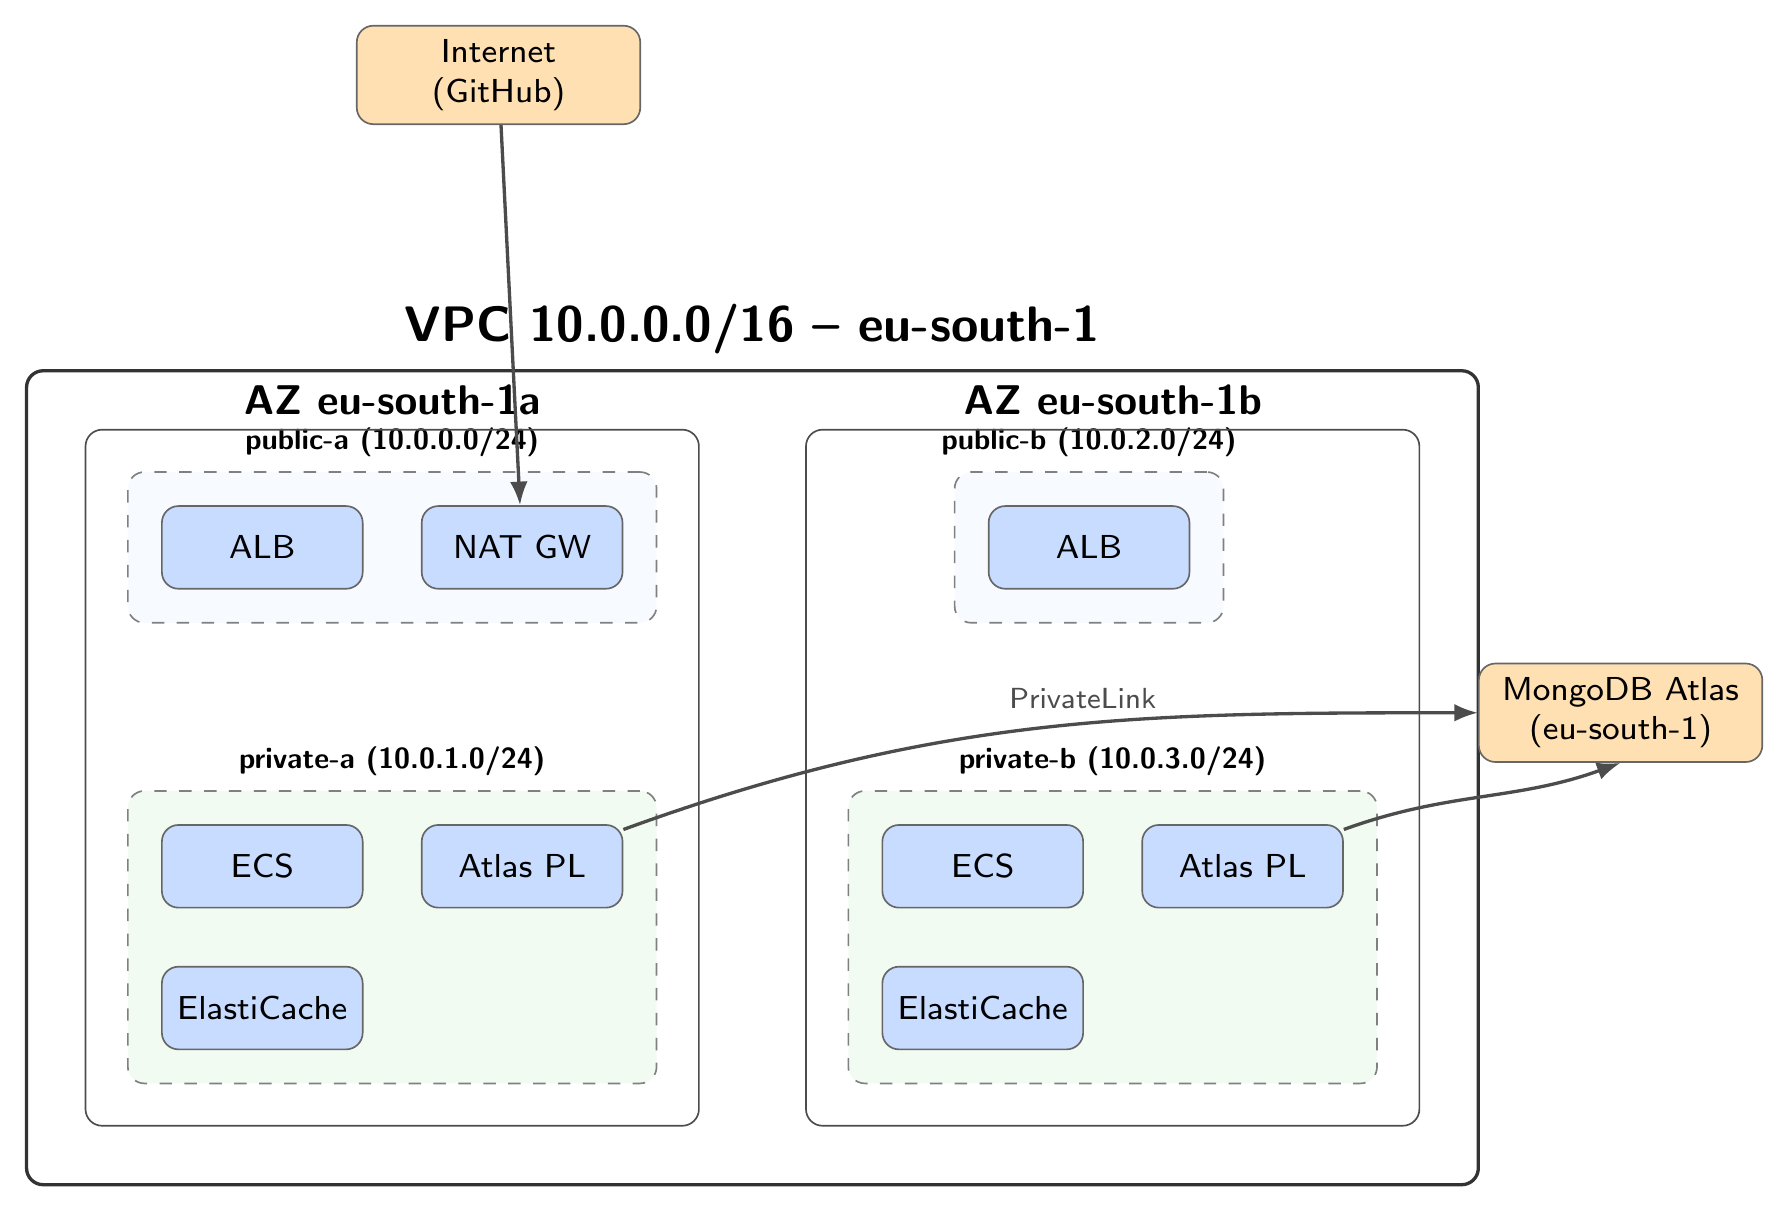
\includegraphics[width=0.85\textwidth]{figures/aws-vpc.png}
\caption[VPC del MVP]{VPC del MVP: due Availability Zone, subnet pubbliche e private, NAT Gateway unico in \texttt{public-a}. Il database MongoDB Atlas è esterno alla VPC e raggiunto via AWS PrivateLink (Interface Endpoint ``Atlas PL'' nelle subnet private). Gli altri VPC Endpoint verso i servizi AWS interni sono omessi da questo diagramma.}
\label{fig:aws-vpc}
\end{figure}

\subsection{VPC Endpoints (PrivateLink)}

Tutto il traffico AWS interno deve restare nella VPC. Il NAT serve esclusivamente per GitHub. Tutti gli Endpoint ``Interface'' richiedono l'abilitazione del Private DNS.

\begin{table}[H]
\centering
\caption{Elenco VPC Endpoints da configurare.}
\label{tab:aws-vpce}
\vspace{2mm}
\renewcommand{\arraystretch}{1.2}
\begin{tabularx}{\textwidth}{|l|l|X|}
\hline
\textbf{Servizio AWS} & \textbf{Tipo} & \textbf{Note Operative} \\ \hline
S3 & Gateway & Agisce su Route Table, no Private DNS necessario. \\ \hline
Bedrock Runtime & Interface & Indispensabile per sicurezza Prompt (ADR-AWS-6, \S~\ref{sec:aws-adr}). \\ \hline
Secrets Manager & Interface & Interrogato dai task all'avvio. \\ \hline
ECR (\texttt{api}, \texttt{dkr}) & Interface & Pull immagini senza uscita web. \\ \hline
CloudWatch Logs & Interface & Traffico streaming logs continuo. \\ \hline
SSM, SSM Msgs, EC2 Msgs & Interface & Necessari per ECS Exec senza Bastion Host (ADR-AWS-7, \S~\ref{sec:aws-adr}). \\ \hline
MongoDB Atlas (PrivateLink) & Interface & Endpoint verso l'\emph{endpoint service} di Atlas (non \texttt{com.amazonaws.*}). Usare la \emph{connection string del Private Endpoint} fornita da Atlas per la risoluzione DNS. \\ \hline
\end{tabularx}
\end{table}

\begin{quote}
\textbf{Nota Implementativa.} Ogni VPC Endpoint di tipo \emph{Interface} viene fatturato per ora \textbf{per ogni AZ} in cui è distribuito. Con 7 endpoint Interface (incluso Atlas PrivateLink) su 2 AZ si tratta di 14 ENI fatturati continuativamente, da includere nella stima con AWS Pricing Calculator (\S~10.2) insieme al NAT Gateway.
\end{quote}

\subsection{Matrice Security Groups (Regole di Rete)}

Ogni componente possiede un SG dedicato. Il traffico non in elenco è implicitamente negato.

\begin{table}[H]
\centering
\caption{Matrice delle Regole Security Group. *L'endpoint Bedrock accetta ingress solo da \texttt{sg-agents}.}
\label{tab:aws-sg}
\vspace{2mm}
\renewcommand{\arraystretch}{1.2}
\begin{tabularx}{\textwidth}{|l|X|X|}
\hline
\textbf{Security Group} & \textbf{Ingress (In Entrata)} & \textbf{Egress (In Uscita)} \\ \hline
\texttt{sg-alb} & TCP 80 dal Prefix List AWS {\ttfamily com.\allowbreak{}amazonaws.\allowbreak{}global.\allowbreak{}cloudfront.\allowbreak{}origin-facing} & TCP 3000 verso \texttt{sg-backend} \\ \hline
\texttt{sg-backend} & TCP 3000 da \texttt{sg-alb} & TCP 27017 verso \texttt{sg-atlas} (endpoint Atlas PrivateLink); TCP 6379 verso \texttt{sg-redis}; TCP 443 verso \texttt{sg-vpce}; Porta interna verso \texttt{sg-agents}; TCP 443 verso \texttt{0.0.0.0/0} (Solo NAT/GitHub) \\ \hline
\texttt{sg-agents} & Porta interna da \texttt{sg-backend} & Porta interna verso \texttt{sg-backend}; TCP 443 verso \texttt{sg-vpce}; \textbf{NESSUNA} regola verso \texttt{0.0.0.0/0} (ADR-AWS-4, \S~\ref{sec:aws-adr}) \\ \hline
\texttt{sg-atlas} & TCP 27017 da \texttt{sg-backend} & (Nessuna regola) \\ \hline
\texttt{sg-redis} & TCP 6379 da \texttt{sg-backend} & (Nessuna regola) \\ \hline
\texttt{sg-vpce} & TCP 443 da \texttt{sg-backend}; TCP 443 da \texttt{sg-agents}* & (Nessuna regola) \\ \hline
\end{tabularx}
\end{table}

\begin{quote}
\textbf{Attenzione.} Il Security Group \texttt{sg-atlas} è associato all'\emph{Interface VPC Endpoint} di Atlas PrivateLink, non a un'istanza database nella VPC. La porta esatta (27017 o l'eventuale range indicato da Atlas) va confermata dalla \emph{connection string del Private Endpoint} generata in fase di pairing e usata come sorgente di verità per le regole di egress di \texttt{sg-backend}.
\end{quote}

\section{Compute e Orchestrazione (ECS su Fargate)}
\label{sec:aws-compute}

Il deploy dell'applicativo si basa sulle stesse immagini Docker validate nel PoC (Parte~\ref{part:poc}), senza modifiche al codice sorgente (Parte~\ref{part:aws-adr}: Principio di Migrazione).

\subsection{Cluster ECS e Task Definition}

\begin{itemize}
    \item \textbf{Capacity Provider:} Esclusivamente \texttt{FARGATE} (nessun \texttt{FARGATE\_SPOT}).
    \item \textbf{Modalità di Rete:} \texttt{awsvpc} (interfacce dedicate nelle subnet private).
    \item \textbf{Log Driver:} \texttt{awslogs} (inoltro standard output/error a CloudWatch Logs).
\end{itemize}

\begin{table}[H]
\centering
\caption{Dimensionamento e configurazione Task ECS per l'MVP.}
\label{tab:aws-ecs}
\vspace{2mm}
\renewcommand{\arraystretch}{1.2}
\begin{tabularx}{\textwidth}{|l|l|l|l|X|}
\hline
\textbf{Servizio ECS} & \textbf{vCPU} & \textbf{Memoria} & \textbf{Desired Count} & \textbf{Configurazioni Task} \\ \hline
\texttt{backend} & 0.5 & 1 GB & 1 (\S~\ref{sec:aws-adr}) & Health check breve su \texttt{/health}. \textbf{Vincolo implementativo}: la generazione PDF deve usare una libreria di composizione programmatica (\textbf{pdfkit}), \textbf{non} rendering via browser headless; dimensionamento da confermare con test di carico su export concorrenti prima del rilascio (\S~\ref{sec:aws-compromessi}, Tabella~\ref{tab:aws-compromessi}). \\ \hline
\texttt{agents} & 1.0 & 2 GB & 1 (\S~\ref{sec:aws-adr}) & Valori di base, aggiornabili dopo test di carico su LangGraph e Bedrock. \\ \hline
\end{tabularx}
\end{table}

\subsection{Gestione Immagini Container (Amazon ECR)}

\begin{table}[H]
\centering
\caption{Configurazione dei registri ECR.}
\label{tab:aws-ecr}
\vspace{2mm}
\renewcommand{\arraystretch}{1.2}
\begin{tabularx}{\textwidth}{|l|X|}
\hline
\textbf{Parametro} & \textbf{Valore / Configurazione} \\ \hline
Repository & \texttt{codeguardian/backend}, \texttt{codeguardian/agents} \\ \hline
Tagging & Uso obbligatorio dello SHA breve del commit (es. \texttt{:a1b2c3d}). Tag \texttt{latest} solo come puntatore di comodo in dev. \\ \hline
Security Scan & Scansione automatica base abilitata al push. \\ \hline
Lifecycle Policy & Mantenere ultime 20 immagini taggate; eliminare immagini untagged vecchie di $>1$ giorno. \\ \hline
Permessi IAM Push & Ruolo CI/CD (\texttt{codeguardian-ci-role}). \\ \hline
Permessi IAM Pull & Task Execution Role di ECS. \\ \hline
\end{tabularx}
\end{table}

\subsection{Application Load Balancer (ALB)}

Nessun dominio custom o certificato TLS è installato sull'ALB (ADR-AWS-8, \S~\ref{sec:aws-adr}).

\begin{table}[H]
\centering
\caption{Configurazione ALB.}
\label{tab:aws-alb}
\vspace{2mm}
\renewcommand{\arraystretch}{1.2}
\begin{tabularx}{\textwidth}{|l|X|}
\hline
\textbf{Parametro} & \textbf{Valore Operativo} \\ \hline
Posizionamento & Subnet pubbliche (\texttt{public-a}, \texttt{public-b}). \\ \hline
Listener & Protocollo HTTP, Porta 80. \\ \hline
Target Group & Tipo \texttt{ip}, Porta 3000, Protocollo HTTP (puntato ai task del backend). Path Health Check: \texttt{/health}. \\ \hline
Idle Timeout & 3600 secondi (Necessario per connessioni WebSocket). \\ \hline
Stickiness & Abilitata, cookie \texttt{AWSALB}, durata 3600 secondi. \\ \hline
Deregistration & 30 secondi (Ridotto per deploy più rapidi). \\ \hline
\end{tabularx}
\end{table}

\subsection{Service Discovery (AWS Cloud Map)}

Usata per la comunicazione interna (Backend $\leftrightarrow$ Agents).

\begin{itemize}
    \item \textbf{Namespace Privato:} \texttt{codeguardian.local} (associato alla VPC).
    \item \textbf{TTL Record DNS:} 10 secondi.
\end{itemize}

\begin{table}[H]
\centering
\caption{Record Service Discovery Cloud Map.}
\label{tab:aws-clmap}
\vspace{2mm}
\renewcommand{\arraystretch}{1.2}
\begin{tabularx}{\textwidth}{|X|l|l|X|}
\hline
\textbf{Servizio DNS} & \textbf{Porta} & \textbf{Tipo} & \textbf{Scopo} \\ \hline
\texttt{agents.codeguardian.local} & 8000 & A & Chiamato dal backend per avvio run. \\ \hline
\texttt{backend.codeguardian.local} & 3000 & A & Chiamato dagli agenti per tool-calls (GitHub read-only) e callback di progresso (ADR-AWS-3, \S~\ref{sec:aws-adr}). \\ \hline
\end{tabularx}
\end{table}

\subsection{Flussi Applicativi End-to-End}

Il diagramma di rete (Figura~\ref{fig:aws-vpc}) mostra il posizionamento delle risorse, non i flussi dati. La Figura~\ref{fig:aws-flussi} integra le due viste, mostrando chi chiama chi e con quale protocollo.

\begin{figure}[H]
\centering
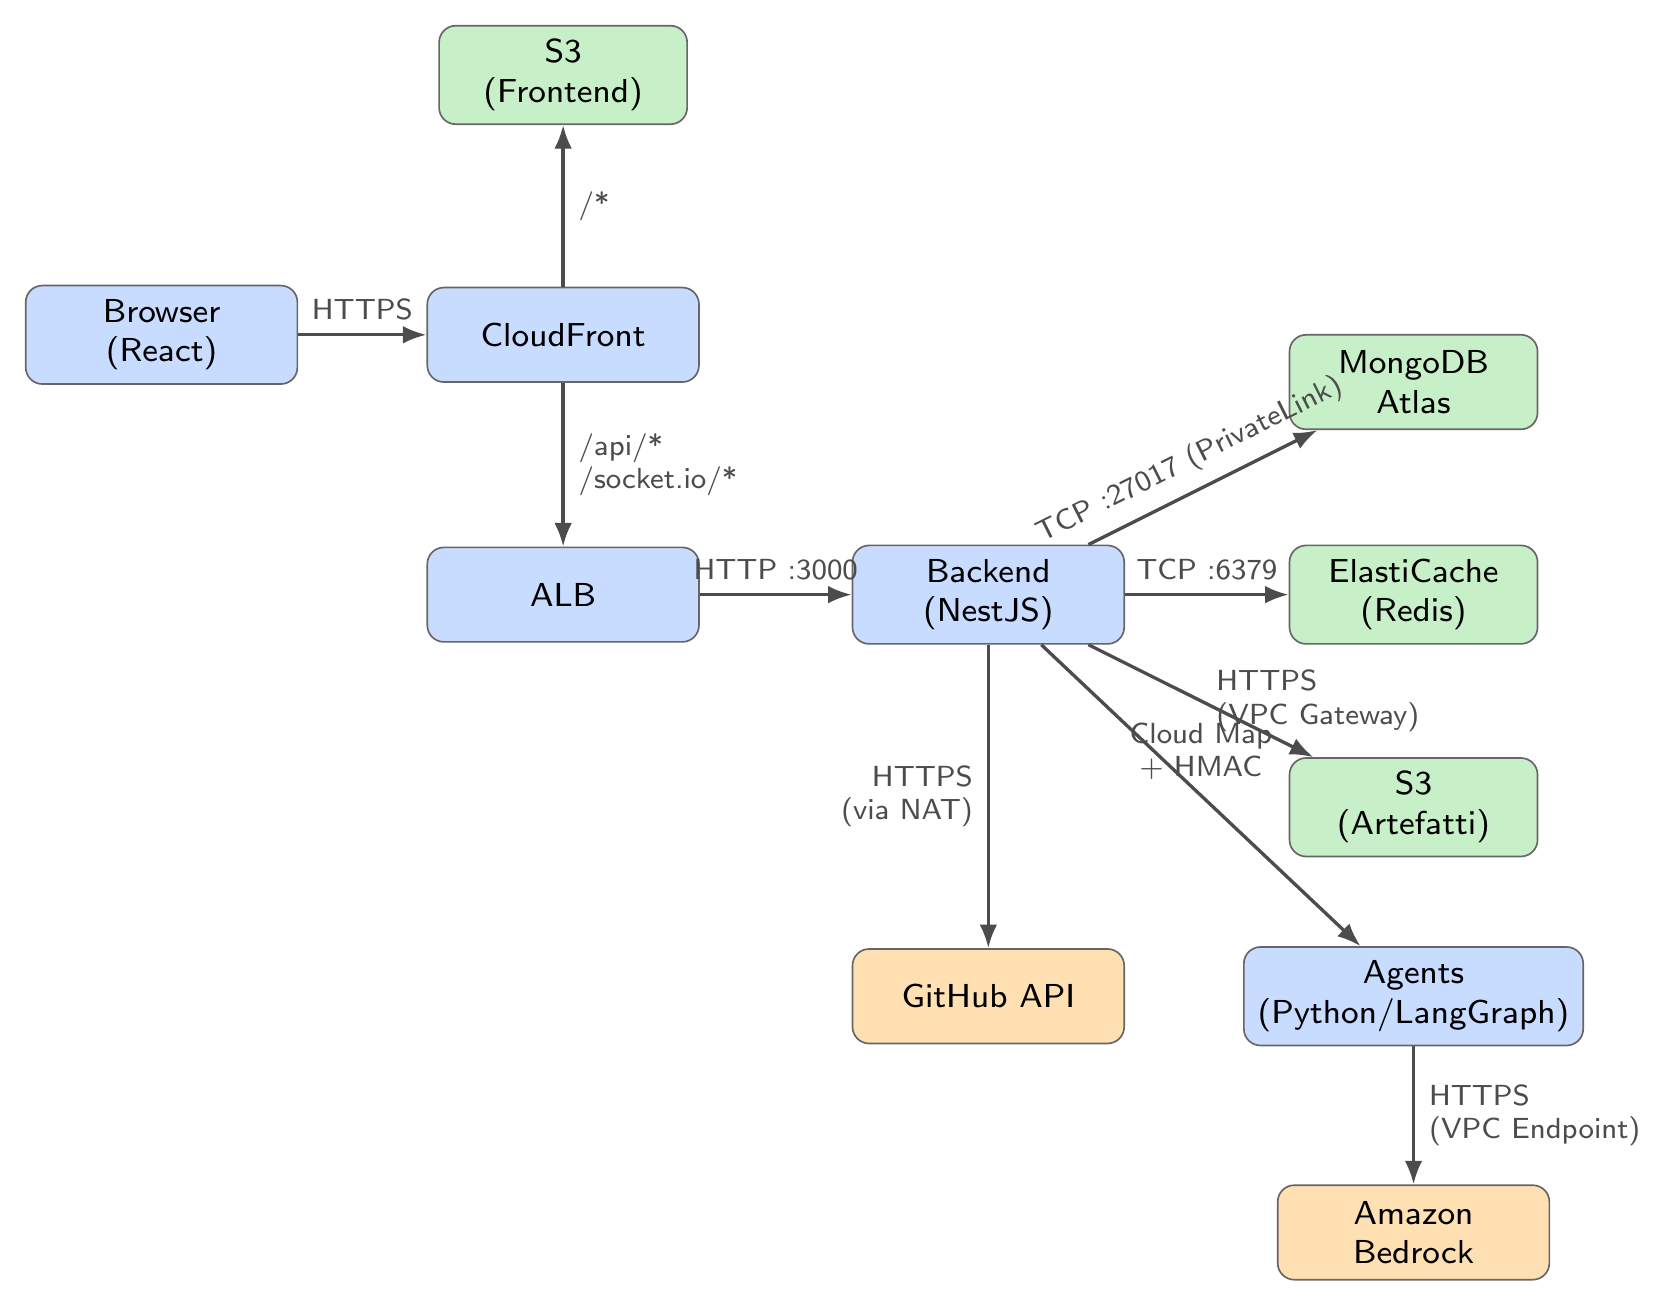
\includegraphics[width=0.95\textwidth]{figures/aws-flussi.png}
\caption[Flussi applicativi principali]{Flussi applicativi principali con protocollo e direzione. Il traffico agents$\to$GitHub non esiste: ogni lettura passa dalla facade del backend (\S~\ref{sec:github}, ADR-AWS-1).}
\label{fig:aws-flussi}
\end{figure}

\section{Livello Dati e Caching}
\label{sec:aws-dati}

\subsection{MongoDB Atlas (via AWS PrivateLink)}

Sostituisce il container MongoDB del PoC con un cluster \textbf{MongoDB Atlas} gestito, deployato su AWS nella regione \texttt{eu-south-1} e raggiunto esclusivamente tramite \textbf{AWS PrivateLink} (nessun transito su Internet pubblico e nessuna dipendenza dal NAT Gateway per il livello dati).

\begin{table}[H]
\centering
\caption{Configurazione MongoDB Atlas.}
\label{tab:aws-atlas}
\vspace{2mm}
\renewcommand{\arraystretch}{1.2}
\begin{tabularx}{\textwidth}{|l|X|}
\hline
\textbf{Parametro} & \textbf{Valore Operativo} \\ \hline
Tier & \texttt{M10} dedicato (minimo che abilita PrivateLink). \\ \hline
Topologia & Replica set a 3 nodi distribuiti sulle AZ della regione (alta disponibilità per costruzione, gestita da Atlas). \\ \hline
Regione & AWS \texttt{eu-south-1} (Milano), per data residency coerente col resto dello stack. \\ \hline
Versione & Ultima major MongoDB supportata da Atlas nella regione. \\ \hline
Connettività & AWS PrivateLink (Interface Endpoint su \texttt{private-a}/\texttt{private-b}); \emph{Network Access List} Atlas ristretta al Private Endpoint. \\ \hline
Rete e Sicurezza & Porta MongoDB (27017), SG \texttt{sg-atlas} sull'endpoint (Ingresso solo da \texttt{sg-backend}). \\ \hline
Cifratura & A riposo gestita da Atlas (AES-256); BYOK via KMS fuori scope MVP. In transito TLS obbligatoria (CA pubblica). \\ \hline
Backup & Atlas Cloud Backup (snapshot gestiti da Atlas, non da AWS Backup). \\ \hline
\end{tabularx}
\end{table}

\begin{quote}
\textbf{Attenzione.} Con PrivateLink la connessione deve usare la \emph{connection string del Private Endpoint} generata da Atlas (host che risolvono a IP privati), \textbf{non} la connection string standard \texttt{mongodb+srv://} pubblica: quest'ultima risolverebbe a IP pubblici non instradabili senza NAT, con connessione in timeout senza un errore esplicito. Atlas usa certificati TLS da CA pubblica: \textbf{non} serve alcun CA bundle custom (a differenza di DocumentDB, che imponeva il bundle RDS).
\end{quote}

\begin{lstlisting}[caption={Connessione Mongoose a MongoDB Atlas (Private Endpoint)}]
// MONGO_URI = connection string del PRIVATE ENDPOINT
// (Atlas -> Connect -> Private Endpoint), es.:
// mongodb+srv://<user>:<pwd>@<cluster>-pl-0.<hash>.mongodb.net/<db>?retryWrites=true

mongoose.connect(process.env.MONGO_URI, {
  // TLS implicito con mongodb+srv; nessun tlsCAFile custom (CA pubblica)
});
\end{lstlisting}

\emph{Azione Dev:} Configurare Private Endpoint e Network Access List su Atlas e verificare la connessione dal task \texttt{backend}. Lo schema design della base dati resta di competenza del team backend (RV.21), senza spike di compatibilità.

\subsection{Amazon ElastiCache (Redis)}

Duplice uso applicativo: coda BullMQ (\texttt{bull:*}) e cache GitHub (\texttt{repo@sha:*}).

\begin{table}[H]
\centering
\caption{Configurazione ElastiCache (Redis).}
\label{tab:aws-redis}
\vspace{2mm}
\renewcommand{\arraystretch}{1.2}
\begin{tabularx}{\textwidth}{|l|X|}
\hline
\textbf{Parametro} & \textbf{Valore Operativo} \\ \hline
Topologia & Nodo singolo (No cluster, no repliche) (\S~\ref{sec:aws-compromessi}). \\ \hline
Subnet Group & Subnet private (\texttt{private-a}, \texttt{private-b}). \\ \hline
Rete e Sicurezza & Porta 6379, SG \texttt{sg-redis} (Ingresso solo da \texttt{sg-backend}). \\ \hline
Cifratura & A riposo abilitata (Stessa chiave KMS), in transito (\texttt{in-transit encryption}) abilitata. \\ \hline
\end{tabularx}
\end{table}

\begin{quote}
\textbf{Attenzione.} Abilitare \texttt{in-transit encryption} su ElastiCache \textbf{non è trasparente} lato applicativo: il client (\texttt{ioredis} / \texttt{node-redis}) deve connettersi specificando esplicitamente l'opzione TLS, altrimenti la connessione fallisce in timeout senza un messaggio di errore chiaro.
\end{quote}

\begin{lstlisting}[caption={Connessione ioredis con TLS abilitato}]
const redis = new Redis({
  host: process.env.REDIS_HOST,
  port: 6379,
  tls: {}, // richiesto se in-transit encryption e' abilitata
});
\end{lstlisting}

\textbf{Rate Limiting Applicativo (RQ.8).} Oltre agli usi già previsti (coda BullMQ, cache letture GitHub), l'istanza Redis supporta un \textbf{rate limiter applicativo} lato backend NestJS con \textbf{sliding window}, con chiave per utente (\texttt{userId}): il limite è fissato a \textbf{60 richieste al minuto per utente} sugli endpoint che invocano l'API GitHub (variabile d'ambiente \texttt{RATE\_LIMIT\_\allowbreak{}GITHUB\_\allowbreak{}RPM=60}). Questo copre RQ.8 con un controllo architetturale reale, senza affidarsi ai soli limiti di default dell'account Bedrock (insufficienti da soli a soddisfare il requisito in modo verificabile). Non introduce nuovi servizi AWS: riusa l'istanza ElastiCache già provisionata.

\section{Integrazione Amazon Bedrock}

Tutte le comunicazioni con Bedrock avvengono via VPC Endpoint, garantendo che il codice analizzato non transiti su Internet pubblico (Conformità RS.5, \S~\ref{sec:aws-adr}).

\subsection{Modelli e Accessi}

L'accesso ai modelli va richiesto \textbf{immediatamente} tramite console Bedrock (sezione \emph{Model access}) nella regione \texttt{eu-south-1}.

\begin{table}[H]
\centering
\caption{Assegnazione Modelli e Richieste di Accesso Bedrock.}
\label{tab:aws-bedrock-modelli}
\vspace{2mm}
\renewcommand{\arraystretch}{1.2}
\begin{tabularx}{\textwidth}{|l|X|X|}
\hline
\textbf{Agente} & \textbf{Modello Selezionato} & \textbf{Priorità di Richiesta} \\ \hline
Docs, Changelog & Qwen3-32B (dense) & Alta (Assegnazione primaria). \\ \hline
Security & Qwen3-Coder-30B-A3B-Instruct & Alta (Assegnazione primaria). \\ \hline
N/A (Scalata) & Qwen3-235B-A22B & Media (Richiedere subito come fallback in caso di accuratezza insufficiente in fase di validazione) (\S~\ref{sec:aws-adr}). \\ \hline
\end{tabularx}
\end{table}

\begin{quote}
\textbf{Attenzione.} Verificare in console Bedrock (sezione \emph{Model access / Cross-region inference}) se i modelli Qwen3 richiedono un \textbf{Inference Profile ARN} invece dell'ARN diretto del foundation model per l'invocazione on-demand. Se richiesto, l'ARN nella policy IAM e nel codice applicativo va aggiornato di conseguenza; l'errore tipico in caso di mismatch è \texttt{ValidationException: Invocation of model ID ... is not supported}.
\end{quote}

\subsection{Autenticazione e Policy IAM}

Nessuna chiave API statica (ADR-AWS-1, \S~\ref{sec:aws-adr}). L'invocazione avviene tramite il Task Role del servizio \texttt{agents}.

\begin{table}[H]
\centering
\caption{Configurazione IAM per l'accesso a Bedrock.}
\label{tab:aws-bedrock-iam}
\vspace{2mm}
\renewcommand{\arraystretch}{1.2}
\begin{tabularx}{\textwidth}{|l|X|}
\hline
\textbf{Parametro Policy} & \textbf{Valore Operativo} \\ \hline
Azioni Ammesse & \texttt{bedrock:InvokeModel}, \texttt{bedrock:InvokeModelWithResponseStream} \\ \hline
Risorse (ARNs) & \texttt{arn:aws:bedrock:eu-south-1::foundation-model/qwen.*} (Scoping limitato alla famiglia Qwen3 per impedire l'uso accidentale di modelli costosi). \\ \hline
Condizioni & \texttt{aws:RequestedRegion == eu-south-1}. \\ \hline
\end{tabularx}
\end{table}

\subsection{Model Invocation Logging}

\begin{itemize}
    \item \textbf{Cosa registrare:} Solo i metadati (Modello invocato, timestamp, token consumati).
    \item \textbf{Cosa NON registrare:} Corpo del prompt e della risposta (per policy di sicurezza sul codice).
    \item \textbf{Vincolo:} Aggiungere resource policy al Log Group per permettere al principal {\ttfamily bedrock.\allowbreak{}amazonaws.com} la scrittura.
\end{itemize}

\section{Storage e Comunicazioni Esterne}

\subsection{Amazon S3 (Artefatti Applicativi)}

Sostituisce MinIO per il salvataggio dei report generati.

\begin{table}[H]
\centering
\caption{Configurazione Bucket S3 (Artefatti).}
\label{tab:aws-s3-artefatti}
\vspace{2mm}
\renewcommand{\arraystretch}{1.2}
\begin{tabularx}{\textwidth}{|l|X|}
\hline
\textbf{Parametro} & \textbf{Valore Operativo} \\ \hline
Accesso di Rete & Nessun accesso pubblico (\texttt{Block Public Access = True}). Accesso solo via VPC Endpoint Gateway. \\ \hline
Permessi IAM & Concessi in lettura/scrittura esclusivamente al Task Role del servizio \texttt{backend}. \\ \hline
Cifratura \& Versioning & Cifratura KMS abilitata. Versioning disabilitato. \\ \hline
Lifecycle Policy & Eliminazione automatica oggetti $>30$ giorni. \\ \hline
\end{tabularx}
\end{table}

\section{Frontend Web Hosting}
\label{sec:aws-frontend-hosting}

Il frontend React (Vite) viene compilato come sito statico. Un'unica distribuzione CloudFront serve sia il Frontend sia le API, eliminando la necessità di configurare policy CORS (ADR-AWS-9, \S~\ref{sec:aws-adr}).

\subsection{Amazon S3 (Hosting Statico)}

\begin{itemize}
    \item \textbf{Accesso Pubblico:} Bloccato. Il Bucket NON deve usare la funzione "Static Website Hosting" nativa.
    \item \textbf{Accesso in Lettura:} Esclusivo per CloudFront tramite Origin Access Control (OAC).
\end{itemize}

\subsection{Distribuzione Amazon CloudFront}

\begin{table}[H]
\centering
\caption{Behavior di CloudFront per l'MVP condiviso.}
\label{tab:aws-cloudfront}
\vspace{2mm}
\renewcommand{\arraystretch}{1.2}
\begin{tabularx}{\textwidth}{|l|l|X|}
\hline
\textbf{Behavior Path} & \textbf{Origin Target} & \textbf{Configurazione e Policy} \\ \hline
\texttt{/*} (Default) & Bucket S3 & \textbf{Viewer Protocol:} Redirect HTTP to HTTPS. \textbf{Cache:} Abilitata. \\ \hline
\texttt{/api/*} e \texttt{/socket.io/*} & ALB (Backend) & \textbf{Viewer Protocol:} HTTP Only (L'ALB non ha certificato TLS). \textbf{Cache:} Disabilitata. \textbf{Origin Request Policy:} Forward All (Inoltro header \texttt{Upgrade}, \texttt{Connection}, e \texttt{Authorization}). \\ \hline
\end{tabularx}
\end{table}

\subsection{Gestione SPA Routing e Build Vite}

\begin{itemize}
    \item \textbf{Custom Error Response (CloudFront):} Errori 403/404 generati da S3 devono essere redirezionati al file \texttt{index.html} con Status Code 200 (necessario per TanStack Router).
    \item \textbf{Variabili Runtime:} Configurare \texttt{VITE\_API\_BASE\_URL} con un path relativo (es. \texttt{/api/v1}) durante la build.
    \item \textbf{Cache Invalidation:} Il ruolo CI/CD deve avere i permessi \texttt{cloudfront:}\linebreak[0]\texttt{CreateInvalidation} per svuotare la cache ad ogni deploy.
\end{itemize}

\section{Segreti e Configurazione (Variabili d'Ambiente)}
\label{sec:aws-config}

\subsection{Mappatura Variabili PoC $\to$ AWS}

Integrazione trasparente: il codice applicativo continua a leggere le variabili tramite \texttt{process.env} / \texttt{os.environ}. La configurazione viene iniettata nativamente da ECS al momento del bootstrap.

\begin{table}[H]
\centering
\caption{Mappatura delle Variabili d'Ambiente.}
\label{tab:aws-env}
\vspace{2mm}
\renewcommand{\arraystretch}{1.15}
\begin{tabularx}{\textwidth}{|l|l|X|X|}
\hline
\textbf{Variabile (PoC)} & \textbf{Servizio} & \textbf{Meccanismo AWS} & \textbf{Permessi Lettura IAM} \\ \hline
\texttt{MONGO\_URI} & backend & Secrets Manager & Task Execution (backend) \\ \hline
\texttt{JWT\_SECRET} & backend & Secrets Manager & Task Execution (backend) \\ \hline
\texttt{CREDENTIAL\_MASTER\_KEY} & backend & Secrets Manager & Task Execution (backend) \\ \hline
\texttt{INTERNAL\_SHARED\_SECRET} & Entrambi & Secrets Manager & Task Exec (backend \& agents) \\ \hline
\texttt{REDIS\_URL} & backend & Parameter Store & Task Execution (backend) \\ \hline
\texttt{BACKEND\_BASE\_URL} & agents & Parameter Store & Task Execution (agents) \\ \hline
\texttt{LLM\_PROVIDER} & agents & Parameter Store & Task Execution (agents) \\ \hline
\multicolumn{4}{|l|}{\textit{Variabili Rimosse o Modificate}} \\ \hline
\texttt{LLM\_API\_KEY}, \texttt{S3\_KEY} & Tutti & ELIMINATE & Sostituite da IAM Task Role. \\ \hline
\texttt{PROMPTS\_DIR} & agents & Bake-in Docker & Niente mount locali in Fargate. \\ \hline
\end{tabularx}
\end{table}

\subsection{Cifratura (AWS KMS)}

Creare un'unica chiave \textbf{KMS Customer Managed Key} per l'MVP.

\begin{itemize}
    \item \textbf{Utilizzatori per cifratura:} Servizio ElastiCache, Secrets Manager, S3. \emph{MongoDB Atlas cifra a riposo con chiavi proprie, fuori da questa CMK.}
    \item \textbf{Utilizzatori per decifratura:} Task Execution Roles di \texttt{backend} e \texttt{agents} (per l'iniezione sicura all'avvio del container).
\end{itemize}

\section{Budget e Osservabilità Infrastrutturale}

\subsection{Metriche e Allarmi Base}

Tutti gli allarmi vanno instradati verso un unico Topic SNS (\texttt{codeguardian-alerts}), condiviso dal team di sviluppo via email.

\begin{table}[H]
\centering
\caption{Matrice degli allarmi infrastrutturali base.}
\label{tab:aws-allarmi}
\vspace{2mm}
\renewcommand{\arraystretch}{1.2}
\begin{tabularx}{\textwidth}{|l|X|X|}
\hline
\textbf{Allarme / AWS Service} & \textbf{Metrica} & \textbf{Soglia di Attivazione} \\ \hline
ECS Fargate & Task in esecuzione & $<1$ (Desired Count) per $>5$ minuti. \\ \hline
ECS Fargate & Utilizzo CPU / Memoria & $>80\%$ per $>5$ minuti. \\ \hline
ALB & Tasso di errore HTTP 5xx & $>5\%$ su finestra di 5 minuti. \\ \hline
ElastiCache & Utilizzo CPU Cache & $>80\%$ per $>5$ minuti. \\ \hline
Amazon Bedrock & Invocation Throttling & $\geq 1$ invocazione limitata in 5 minuti. \\ \hline
\end{tabularx}
\end{table}

\begin{quote}
\textbf{Nota Implementativa.} Le metriche del cluster \textbf{MongoDB Atlas} (CPU, connessioni, IOPS, replication lag) non sono esposte nativamente su CloudWatch: gli allarmi relativi si configurano con l'\emph{alerting integrato di Atlas}, instradato verso lo stesso canale del team (email o, opzionalmente, integrazione Atlas $\to$ SNS/webhook). CloudWatch resta autoritativo per ECS, ALB, ElastiCache e Bedrock.
\end{quote}

\textbf{Correlazione dei Log tra Servizi.} Ogni log strutturato emesso da \texttt{backend} e \texttt{agents} deve includere il campo \texttt{taskId} (già presente nel modello di dominio del PoC) in ogni riga, per l'intera durata dell'esecuzione di una Task. Questo consente di filtrare CloudWatch Logs Insights per una singola run end-to-end (avvio, tool-call verso GitHub, invocazione Bedrock, persistenza del Report) senza introdurre un sistema di tracing distribuito dedicato, non giustificato nei tempi dell'MVP.

\subsection{Gestione Costi (AWS Budgets)}

\emph{Azione Dev:} Usare AWS Pricing Calculator per ottenere il Costo Mensile Stimato basato sui parametri di questo documento (1 NAT, 1 ElastiCache, 7 VPC Endpoint --- incluso Atlas PrivateLink ---, Compute ECS). \textbf{Il costo del cluster MongoDB Atlas M10 è fatturato separatamente da MongoDB} (non compare in AWS Pricing Calculator) e va sommato alla stima; l'Interface Endpoint di PrivateLink è invece un costo AWS.

\begin{itemize}
    \item \textbf{Soglia 50\%:} Informativa (Nessuna azione richiesta).
    \item \textbf{Soglia 80\%:} Attenzione (Indagare eventuali loop di esecuzione).
    \item \textbf{Soglia 100\%:} Superamento budget (Nessun blocco automatico configurato per evitare downtime bloccanti).
\end{itemize}

\section{Tracciamento Requisito $\to$ Decisione AWS}

Questa tabella mappa i requisiti funzionali, di vincolo e qualitativi (definiti nell'Analisi dei Requisiti) sulle scelte operative AWS implementate in questa configurazione. I requisiti puramente applicativi restano di competenza dello sviluppo software.

\begin{center}
\footnotesize
\renewcommand{\arraystretch}{1.15}
\begin{xltabular}{\textwidth}{|l|X|X|l|}
\caption{Mappatura Requisiti - Decisioni Infrastrutturali AWS.}
\label{tab:aws-req-decisioni} \\
\hline
\textbf{Requisito} & \textbf{Descrizione Sintetica} & \textbf{Decisione Infrastrutturale (AWS)} & \textbf{Rif.} \\ \hline
\endfirsthead
\multicolumn{4}{l}{\normalsize\itshape Tabella~\ref{tab:aws-req-decisioni} (segue dalla pagina precedente)} \\
\hline
\textbf{Requisito} & \textbf{Descrizione Sintetica} & \textbf{Decisione Infrastrutturale (AWS)} & \textbf{Rif.} \\ \hline
\endhead
\hline
\multicolumn{4}{r}{\normalsize\itshape (continua)} \\
\endfoot
\hline
\endlastfoot
RV.15 & Architettura e hosting basati su AWS. & Compute e servizi core su AWS: VPC, ECS (Fargate), ElastiCache, Bedrock, S3, CloudFront. Il database è MongoDB Atlas, servizio gestito di terze parti \emph{deployato su AWS} in \texttt{eu-south-1} e raggiunto via PrivateLink: hosting su AWS e data residency preservati, con una dipendenza da fornitore esterno (\S~\ref{sec:aws-compromessi}). & Tutto il doc. \\ \hline
RV.12 & Database non relazionale basato su MongoDB. & Adozione di MongoDB Atlas (cluster M10, MongoDB nativo) in \texttt{eu-south-1}, connesso via AWS PrivateLink. & \S~5 \\ \hline
RV.13 & Interfacciamento con LLM tramite AWS Bedrock. & Invocazione nativa Bedrock tramite Task Role IAM del container \texttt{agents}, via VPC Endpoint. & \S~6 \\ \hline
RV.21 & Schema Design della base dati non relazionale. & Demandato al team backend. Nessuno spike di compatibilità richiesto: Atlas è MongoDB nativo (driver Mongoose pienamente supportato). & \S~5 \\ \hline
RV.4 & Supporto a Repository privati, oltre ai pubblici. & Token GitHub cifrato in AWS Secrets Manager (RS.2), letto dal backend via Task Execution Role; l'accesso in HTTPS verso l'API GitHub avviene tramite il NAT Gateway, indipendentemente dalla visibilità del repository. & \S~3, \S~9 \\ \hline
RV.14 & Integrazione nativa con GitHub e GitHub Issues. & Nessun servizio AWS dedicato: il backend raggiunge le API GitHub in HTTPS in uscita (\texttt{sg-backend} $\to$ NAT Gateway), unico canale esterno oltre a Bedrock. & \S~3 \\ \hline
RS.2 & Token e credenziali memorizzati in formato cifrato. & Segreti instradati su AWS Secrets Manager, cifrati con KMS e iniettati nativamente da ECS al bootstrap. & \S~9 \\ \hline
RS.3 & Divieto di scrittura autonoma agenti su Git. & Il Security Group \texttt{sg-agents} blocca in uscita tutto il traffico Internet (\texttt{0.0.0.0/0}). Letture e scritture (apertura Pull Request) sono eseguite esclusivamente dal backend, mai dagli agenti. & \S~3, \S~13 \\ \hline
RS.5 & Non utilizzo codice per addestramento LLM terzi. & Transito tramite VPC Endpoint e invocazione via Bedrock, coperto dalla garanzia contrattuale AWS. & \S~6 \\ \hline
RQ.4 & Disaccoppiamento prompt dalla logica backend. & I prompt restano file esterni, ma il vincolo Fargate impone il bake-in nell'immagine Docker a ogni modifica. & \S~9, \S~\ref{sec:aws-limiti-piattaforma} \\ \hline
RQ.5 & Accuratezza risposte agenti $\geq 85\%$. & Configurazione di modelli adeguati (Qwen3-Coder) e predisposizione di percorsi di scalata (Qwen3-235B). & \S~6 \\ \hline
RQ.6 & Tempo di risposta agente $\leq 5$ minuti. & Adozione di ECS su Fargate al posto di AWS Lambda, incompatibile con lunghe esecuzioni o WebSocket. & \S~4 \\ \hline
RV.6 & Limitazione budget API. & Alert AWS Budgets su 3 soglie; limitazione della Policy IAM Bedrock alla sola famiglia Qwen3. & \S~10 \\ \hline
RQ.8 & Rate Limiting token API. & Rate limiter applicativo su Redis (\textbf{sliding window, 60 req/min per utente}) lato backend, a protezione delle chiamate verso l'API GitHub; i limiti di account Bedrock restano una difesa di secondo livello, non il controllo primario. & \S~5 \\ \hline
\end{xltabular}
\end{center}

\subsection*{Requisiti Fuori Perimetro Infrastrutturale}

I seguenti requisiti non compaiono in tabella poiché la loro soddisfazione dipende interamente dal codice sorgente o dalle policy di progetto, e non richiedono specifiche risorse o configurazioni AWS:

\begin{itemize}
    \item \textbf{RV.1:} Natura deterministica dell'orchestratore.
    \item \textbf{RV.7:} Analisi supportata per TypeScript, JavaScript, Python.
    \item \textbf{RS.1:} Hashing password utente con \textbf{argon2id} (raccomandazione OWASP 2023; supportato in NestJS tramite il pacchetto \texttt{argon2}).
    \item \textbf{RS.4:} Validità logica delle credenziali Git esterne.
    \item \textbf{RV.16 -- RV.20:} Vincoli di documentazione di progetto, Swagger, e versionamento codice.
\end{itemize}

\part{Infrastruttura AWS --- Motivazioni e Decisioni Architetturali}
\label{part:aws-adr}

\emph{Questa parte raccoglie le argomentazioni, i principi guida e le decisioni architetturali che hanno portato alla configurazione descritta nella Parte~\ref{part:aws-manuale}.}

\section{Principi Guida e Vincoli di Progetto}
\label{sec:aws-principi}

Le scelte architetturali di questo MVP sono state guidate da un set di vincoli e principi applicati trasversalmente a tutti i livelli dell'infrastruttura. Invece di ribadirli per ogni singolo servizio, vengono dichiarati qui come fondamento delle decisioni successive.

\begin{itemize}
    \item \textbf{Vincolo Tempo/Risorse (Il costo operativo):} Il team di sviluppo è composto da 6 persone con meno di due settimane per l'intera implementazione (infrastruttura inclusa). Questo ha imposto la scelta sistematica di servizi gestiti (es. Fargate al posto di EC2) e di topologie minimamente valide (es. singola istanza dati, singolo NAT) per abbattere il tempo di configurazione e manutenzione.
    \item \textbf{Principio di Migrazione (``Code-Freeze'' infrastrutturale):} Nessuna sostituzione infrastrutturale deve toccare il codice applicativo o la logica di business. Le immagini Docker di \texttt{backend} e \texttt{agents} validate nel PoC (Parte~\ref{part:poc}) restano le unità di deploy. L'adattamento avviene esclusivamente tramite iniezione di variabili d'ambiente e interfacce compatibili (es. MongoDB Atlas gestito al posto del container MongoDB del PoC, con lo stesso driver Mongoose).
    \item \textbf{Sicurezza Garantita per Costruzione vs Dichiarata:} Se un vincolo applicativo impone una restrizione (es. divieto di scrittura su GitHub per gli agenti), questo viene garantito a livello di rete (Security Groups, Routing) e non affidato unicamente alla correttezza del codice Python.
    \item \textbf{Infrastructure as Code (AWS CDK in TypeScript):} CDK è stato scelto rispetto a Terraform/HCL poiché il team possiede già una buona padronanza di TypeScript (React, NestJS). Inserire un nuovo linguaggio dichiarativo avrebbe impattato negativamente sul tempo di sviluppo.
\end{itemize}

\section{Decisioni Architetturali (ADR) e Motivazioni}
\label{sec:aws-adr}

Di seguito vengono espanse e contestualizzate le decisioni architetturali cardine (ADR-AWS), raggruppate per dominio di competenza.

\subsection{Identità, Accessi e Segreti}

\begin{itemize}
    \item \textbf{ADR-AWS-1 --- Nessuna chiave statica a lungo termine:} L'autenticazione verso i servizi AWS (Bedrock, S3, ECR) avviene esclusivamente tramite \textbf{IAM Task Roles}. È un miglioramento netto rispetto al PoC: le credenziali sono temporanee, auto-ruotanti e mai esposte nel codice. Si separano inoltre i ruoli di esecuzione (Task Execution Role per pull immagini/segreti) da quelli applicativi (Task Role).
    \item \textbf{ADR-AWS-5 --- Singola Chiave KMS Condivisa:} Cifratura a riposo applicata a ElastiCache, S3 e Secrets Manager tramite un'unica chiave gestita dal cliente (MongoDB Atlas cifra a riposo con chiavi proprie, fuori da questa CMK). Un'architettura a chiavi isolate per servizio offrirebbe una limitazione del danno superiore, ma moltiplicherebbe la complessità delle policy IAM, compromesso non giustificato per un MVP di questa scala.
    \item \textbf{ADR-AWS-10 --- Scrittura su GitHub: esclusivamente dal backend, mai dagli agenti:} La generazione automatica di Pull Request (RF.82, RF.83, RF.86) richiede un token GitHub con scope di scrittura (\texttt{repo}). Per non violare RS.3, l'apertura della PR non è mai eseguita dall'agente Python: l'agente produce solo una \texttt{Proposal} (diff) tramite la facade read-only esistente; è il backend NestJS, ricevuto l'output dell'agente, a invocare l'endpoint di scrittura delle API GitHub. L'isolamento di rete di \texttt{sg-agents} (zero egress) resta invariato: il confine di sicurezza non è lo scope del token ma il fatto che gli agenti non possiedono alcun percorso di rete verso l'esterno, nemmeno per la scrittura. La validazione umana della modifica proposta avviene interamente su GitHub (UC26.2.4/RF.63): il sistema non implementa un flusso di approvazione interno per questa operazione.
\end{itemize}

\subsection{Rete, Sicurezza e Isolamento}

\begin{itemize}
    \item \textbf{ADR-AWS-2 e ADR-AWS-4 --- Isolamento del livello dati e degli Agenti:} Redis (ElastiCache) risiede in subnet private senza IP pubblico; il database MongoDB Atlas è esterno alla VPC ma raggiunto esclusivamente via \textbf{AWS PrivateLink} (Interface Endpoint privato nelle subnet, nessun transito su Internet pubblico né dipendenza dal NAT). Il container \texttt{agents} non possiede alcuna route (nemmeno tramite NAT) verso \texttt{0.0.0.0/0}. Questo rende impossibile per un agente contattare autonomamente GitHub o server esterni, garantendo il vincolo \textbf{RS.3} direttamente a livello di rete.
    \item \textbf{ADR-AWS-6 --- Bedrock via PrivateLink:} Il modello LLM viene interrogato via VPC Endpoint Interface. Questo garantisce che il codice sorgente contenuto nei prompt non transiti mai su Internet pubblico, soddisfacendo la conformità sulla data residency e privacy.
    \item \textbf{ADR-AWS-7 --- Debugging via ECS Exec:} L'accesso shell ai container per il debug avviene tramite AWS Systems Manager (SSM) Session Manager. Non vengono creati Bastion Host né utilizzate chiavi SSH. Questo elimina la vulnerabilità classica di istanze intermedie dimenticate aperte.
    \item \textbf{Scelta di Routing (Singolo NAT e 2 AZ):} Si adottano due Availability Zone poiché rappresentano il minimo tecnico richiesto dall'ALB. Si adotta un singolo NAT Gateway in \texttt{public-a} per contenere i costi continui. In caso di fail della AZ-A, il backend perderebbe temporaneamente l'accesso a GitHub. È un compromesso calcolato e accettato per la scala dell'MVP.
\end{itemize}

\subsection{Compute, Orchestrazione e Frontend}

\begin{itemize}
    \item \textbf{Perché Fargate e non Lambda/EC2:} EC2 è stato escluso per azzerare il tempo di amministrazione OS/host. Lambda è stato escluso poiché gli agenti hanno timeout lunghi (fino a 5 min) con stati conversazionali complessi (LangGraph), e il backend richiede connessioni WebSocket persistenti, pattern incompatibili col paradigma Lambda.
    \item \textbf{Desired Count pari a 1:} Mantenere 1 task per servizio semplifica drasticamente l'MVP. Scaling orizzontale del backend richiederebbe l'introduzione di sticky-sessions sull'ALB o un adapter Redis per la sincronizzazione dei WebSocket.
    \item \textbf{ADR-AWS-3 --- Traffico interno via Cloud Map:} Il traffico tra backend e agenti avviene internamente tramite Service Discovery (namespace \texttt{.local}) protetto da HMAC. Questo evita di esporre API riservate del backend sull'Application Load Balancer pubblico.
    \item \textbf{ADR-AWS-8 e ADR-AWS-9 --- ALB dietro CloudFront condiviso:} Il perimetro esclude l'acquisto di un dominio custom. L'ALB non può quindi ottenere un certificato SSL valido e ascolta in chiaro su porta 80. Viene posto dietro una distribuzione CloudFront (che fornisce TLS nativo gratis su dominio \texttt{*.cloudfront.net}) e l'ALB accetta traffico unicamente dai prefix-list di AWS Edge. Servendo sia S3 (Frontend) che ALB (Backend) sotto lo stesso dominio CloudFront, si rende il traffico \emph{Same-Origin}, azzerando totalmente le configurazioni e i bug relativi alle policy CORS.
\end{itemize}

\subsection{Scelte sul Livello Dati}

\begin{itemize}
    \item \textbf{MongoDB Atlas (gestito, esterno ad AWS):} Sostituisce il container MongoDB locale del PoC. Essendo MongoDB nativo, elimina il rischio di compatibilità sul driver e lo spike di validazione che DocumentDB avrebbe imposto. Il compromesso si sposta sulla natura del servizio: Atlas è un \emph{data processor} di terze parti, mitigato deployandolo su AWS in \texttt{eu-south-1} e raggiungendolo via PrivateLink (traffico sul backbone privato AWS, data residency preservata). Resta una dipendenza da fornitore esterno con fatturazione separata.
    \item \textbf{Disponibilità del livello dati:} Il cluster Atlas M10 è un replica set a 3 nodi multi-AZ, quindi \textbf{HA per costruzione}: il database non è più un SPOF a istanza singola come con DocumentDB. Resta invece single-node \textbf{ElastiCache (Redis)}, senza repliche in questa fase; l'alta disponibilità della cache è esclusa dallo scope per motivi di budget e tempo.
\end{itemize}

\subsection{Scelta dei Modelli LLM (Bedrock)}

\begin{itemize}
    \item \textbf{Esclusione di Llama 3.3 70B:} Il modello usato nel PoC non ha endpoint di inferenza nativi nella regione \texttt{eu-south-1} su Bedrock. Abilitarlo implicherebbe il routing del codice sorgente analizzato verso regioni USA (\emph{cross-region inference}), violando i principi di data residency e incrementando i costi operativi.
    \item \textbf{Adozione di Qwen3 (32B e 30B Coder):} Si adotta la famiglia Qwen3, nativa su Milano e in linea con il budget (\$0.15/\$0.60 per 1M token). L'agente Security sfrutta il modello \texttt{Qwen3-Coder-30B-A3B-Instruct} (MoE) che vanta un reliability score del 76.6\% sul benchmark BFCL-v2 per il tool-calling, un requisito fondamentale per far sì che l'agente decida autonomamente quali file interrogare.
    \item \textbf{Fallback Plan:} Qualora il modello da 30B fallisse i test di accuratezza sul golden set (Piano di Qualifica), il team effettuerà la scalata su \texttt{Qwen3-235B-A22B}, sempre disponibile in \texttt{eu-south-1} per mantenere la conformità, con un modesto aumento dei costi.
\end{itemize}

\section{Compromessi e Rischi Accettati}
\label{sec:aws-compromessi}

Il vincolo temporale per lo sviluppo dell'MVP ha reso necessario bilanciare la perfezione architetturale con il pragmatismo del rilascio. Invece di disseminare queste giustificazioni in ogni capitolo, vengono consolidate nella seguente tabella, che mappa i compromessi infrastrutturali accettati e il relativo Single Point of Failure (SPOF) o limite di sicurezza.

\begin{center}
\footnotesize
\renewcommand{\arraystretch}{1.15}
\begin{xltabular}{\textwidth}{|X|X|X|}
\caption{Matrice dei Compromessi e Rischi Accettati per l'MVP.}
\label{tab:aws-compromessi} \\
\hline
\textbf{Risorsa / Scelta} & \textbf{Compromesso Architetturale} & \textbf{Rischio Accettato} \\ \hline
\endfirsthead
\multicolumn{3}{l}{\normalsize\itshape Tabella~\ref{tab:aws-compromessi} (segue dalla pagina precedente)} \\
\hline
\textbf{Risorsa / Scelta} & \textbf{Compromesso Architetturale} & \textbf{Rischio Accettato} \\ \hline
\endhead
\hline
\multicolumn{3}{r}{\normalsize\itshape (continua)} \\
\endfoot
\hline
\endlastfoot
NAT Gateway & Deployment di un singolo NAT Gateway allocato nella subnet \texttt{public-a} invece di uno per ogni Availability Zone. & Se la AZ \texttt{eu-south-1a} dovesse subire un disservizio, gli agenti perderebbero la connettività per leggere da GitHub. Lato frontend, l'errore è gestito come fallimento generico di orchestrazione (UC23), distinto da un errore di credenziale. \\ \hline
Ridondanza Compute & Subnet e ALB predisposti su 2 AZ, ma \texttt{Desired Count: 1} per ogni servizio ECS: ogni servizio gira comunque su una sola istanza, in una sola AZ, alla volta. La topologia multi-AZ è quindi predisposizione di rete, non protezione attiva contro il fallimento del task. & In caso di crash del task o di disservizio sull'AZ ospitante, il servizio è irraggiungibile fino al riavvio automatico di ECS (nessun failover immediato su AZ alternativa). Rischio della stessa natura di quello già accettato per Auto-Scaling, qui esplicitato separatamente perché riguarda la distribuzione geografica, non solo il numero di repliche. \\ \hline
ElastiCache (Redis) & Nodo singolo (nessuna replica, no modalità cluster). Il DB su Atlas M10 è invece multi-AZ e non è più un SPOF. & SPOF residuo limitato a cache e coda BullMQ. Cluster ElastiCache Multi-AZ non giustificato per un carico da validazione MVP. \\ \hline
MongoDB Atlas (fornitore esterno) & Database gestito da terze parti, fuori dall'account AWS, con fatturazione separata e piano di controllo non gestito via CDK. & Dipendenza da un provider esterno e da PrivateLink per la connettività. Data residency preservata (deploy su AWS \texttt{eu-south-1}); un disservizio di Atlas o del Private Endpoint interrompe il livello dati. \\ \hline
AWS KMS & Utilizzo di un'unica chiave crittografica condivisa per ElastiCache, S3 e Secrets Manager. & Una compromissione della chiave esporrebbe questi livelli di persistenza AWS (MongoDB Atlas cifra a riposo separatamente). Si evitano complessità e moltiplicazione delle policy IAM. \\ \hline
Application Load Balancer & ALB senza certificato TLS pubblico e senza dominio custom, in ascolto solo su HTTP/80 (dietro CloudFront). Conseguenza diretta dell'esclusione del Dominio Custom (Route53) dal perimetro MVP (\S~2.2): senza un dominio proprio non è possibile emettere un certificato ACM valido per l'ALB. & Il tratto di rete tra l'edge CloudFront e l'ALB non è cifrato (traffico comunque ristretto alla rete privata AWS, non instradato su Internet pubblico). Il rischio è accettato in coerenza con la decisione di non acquistare un dominio per l'MVP (ADR-AWS-8); introdurlo richiederebbe di riaprire quella decisione, non solo di configurare un certificato. \\ \hline
Auto-Scaling & Desired count fisso a 1 per i servizi ECS. Nessuna policy di autoscaling configurata. & Irraggiungibilità momentanea in caso di task failure durante il tempo di riavvio (Drop SLA). La resilienza (retry, risincronizzazione post-riconnessione) è responsabilità applicativa backend/frontend, da definire nell'MVP riusando l'approccio del PoC. \\ \hline
AWS WAF & Nessun Web Application Firewall configurato a livello Edge (CloudFront/ALB). & Nessuna protezione infrastrutturale contro DDoS Layer 7 o abusi di throttling applicativo da client anomali. \\ \hline
Token GitHub & Token unico con scope di scrittura (\texttt{repo}), condiviso tra letture e apertura PR. Nessuna segmentazione read/write a livello di credenziale. & Una compromissione del backend (unico detentore del token decifrato) consentirebbe scritture sul repository. Il rischio è mitigato dall'isolamento di rete degli agenti e dalla cifratura KMS del token in Secrets Manager, ma non eliminato: non c'è un secondo token a permessi ridotti per le sole letture. \\ \hline
Backend --- Sizing task per PDF & Task backend dimensionato per un servizio REST leggero (0.5 vCPU / 1 GB, Tabella~\ref{tab:aws-ecs}), esteso senza revisione dedicata a generare e streammare PDF nello stesso container. & Non verificato dal team se il carico di generazione PDF (specialmente in concorrenza con task WebSocket attivi) rientri nel budget di memoria. Rischio contenuto se la generazione usa una libreria non basata su browser headless; da confermare con un test di carico mirato prima del rilascio, non con un ridimensionamento preventivo. \\ \hline
\end{xltabular}
\end{center}

\section{Limiti di Piattaforma (Fargate e Prompt)}
\label{sec:aws-limiti-piattaforma}

Il PoC consentiva la modifica in tempo reale dei prompt passati ai modelli LLM grazie al montaggio di volumi (\emph{bind mount}) da file system locale su Docker Compose. \textbf{AWS Fargate non supporta i bind mount da directory locali.} Per evitare l'introduzione di un file system condiviso (Amazon EFS), che comporterebbe costi continui e overhead di configurazione ingiustificati per l'MVP, \textbf{i file dei prompt devono essere inclusi staticamente (bake-in) all'interno dell'immagine Docker}.

\begin{quote}
\emph{Conseguenza operativa:} Il disaccoppiamento logico richiesto da \textbf{RQ.4} resta soddisfatto (i prompt sono file YAML isolati dal codice Python), ma ogni modifica al testo di un prompt richiederà ora la ricompilazione dell'immagine e un nuovo deploy del servizio \texttt{agents}.
\end{quote}

Il tuning effettivo dei prompt avviene comunque in locale via Docker Compose (bind mount, come nel PoC): il bake-in impatta solo la promozione di una versione già validata verso l'ambiente Fargate, non il ciclo di iterazione. Un'alternativa a costo contenuto (prompt su S3, scaricati a runtime) resta valutabile in una fase successiva, se il tuning dovesse richiedere iterazione diretta contro Fargate/Bedrock.


% ==========================================
% PARTE V: PROGETTAZIONE BACKEND MVP
% ==========================================
\part{Progettazione Backend MVP}
\label{part:backend-mvp}

\section{Perimetro e obiettivo}
\label{sec:be-perimetro}

Questa parte documenta la progettazione del backend per la versione MVP di Code Guardian, a cura di Sara Ristovic (2026/08/14). Estende e sostituisce il contratto PoC descritto nella Parte~\ref{part:poc} per tutti i componenti portati a maturità nell'MVP: autenticazione reale, cifratura delle credenziali di servizio, evoluzione del contratto \texttt{CreateContextDto}, validazione del contesto in otto passi e il meccanismo di interazione asincrona tra l'agente Changelog e l'utente.

Il backend è implementato in NestJS (Node.js/TypeScript). Gli agenti Python (LangGraph) comunicano con il backend tramite HTTP interno su endpoint \texttt{/internal/*} autenticati via HMAC, come già stabilito nel PoC (Parte~\ref{part:poc}, \S~\ref{sec:github}).

\subsection{Cosa cambia dal PoC all'MVP}

\begin{table}[H]
\centering
\caption{Mappatura delle evoluzioni PoC $\to$ Backend MVP.}
\label{tab:be-mappatura}
\vspace{2mm}
\renewcommand{\arraystretch}{1.2}
\begin{tabularx}{\textwidth}{|X|X|}
\hline
\textbf{PoC} & \textbf{MVP} \\ \hline
Auth stub (JWT statico, nessun utente reale) & Auth reale: Argon2id + JWT HS256, registrazione e login effettivi (BE-ADR-1, BE-ADR-5) \\ \hline
Nessuna cifratura credenziali applicativa & AES-256-GCM con chiave derivata via HKDF (BE-ADR-2) \\ \hline
\texttt{CreateContextDto}: \texttt{repoOwner} + \texttt{repoName} + \texttt{ref} & \texttt{CreateContextDto}: \texttt{repoUrl} + \texttt{branch} + \texttt{commitSha?} (BE-ADR-4) \\ \hline
Nessuna validazione del contesto & Sequenza di 8 passi di validazione su \texttt{POST /contexts} \\ \hline
\texttt{AnalysisContextDto} senza \texttt{branch} & \texttt{AnalysisContextDto} include il campo \texttt{branch} \\ \hline
4 eventi WebSocket & 5 eventi WebSocket (aggiunto \texttt{task.inputRequired}) \\ \hline
Nessun input utente a runtime & \texttt{POST /tasks/:id/input} + meccanismo pause/resume LangGraph \\ \hline
3 OperationCode nell'AgentRegistry & 7 OperationCode nell'AgentRegistry \\ \hline
\end{tabularx}
\end{table}

\section{Autenticazione e Autorizzazione}
\label{sec:be-auth}

L'MVP implementa un sistema di autenticazione stateless basato su Argon2id per la verifica della password e JWT HS256 per i token di sessione. Non esiste un server-side token store: il logout è stateless (il client elimina il token). I ruoli utente sono codificati nel claim JWT e verificati da una \texttt{RolesGuard} NestJS.

\subsection{Data Transfer Object}

\begin{lstlisting}[caption={DTO di autenticazione. \texttt{lastName} è un campo obbligatorio nuovo rispetto al PoC; lo schema Mongoose deve includere \texttt{@Prop(\{required:true, trim:true\}) lastName: string}. La risposta di login restituisce solo \texttt{accessToken}; il profilo completo si ottiene con \texttt{GET /auth/me}.}]
// --- Body di POST /auth/register ---
interface RegisterDto {
  firstName: string    // 1-40 caratteri
  lastName: string     // 1-40 caratteri  [campo nuovo MVP]
  email: string        // email valida, univoca
  password: string     // min 8 char, almeno 1 lettera + 1 cifra
  role: UserRole       // scelto alla registrazione, non modificabile
}

type UserRole = 'DEVELOPER' | 'SECURITY_AUDITOR' | 'PROJECT_MANAGER'

// --- Risposta di POST /auth/register (201, senza token) ---
interface UserProfileDto {
  id: string
  firstName: string
  lastName: string
  email: string
  role: UserRole
}

// --- Risposta di POST /auth/login e GET /auth/me ---
// Login restituisce solo il token; il profilo si ottiene con GET /auth/me
interface AuthTokenDto {
  accessToken: string  // JWT HS256, scadenza 8h
}

// UserProfileDto e' la risposta anche di GET /auth/me (stesso schema sopra)

// --- Body di POST /auth/login ---
interface LoginDto {
  email: string
  password: string
}

// --- POST /auth/logout: nessun body, risponde 204 ---
// L'endpoint esiste per consentire al frontend di gestire
// errori di rete espliciti al logout; non ha effetto lato server.
\end{lstlisting}

\subsection{Hashing delle password}

Le password vengono hashate con \textbf{Argon2id} prima della persistenza. I parametri scelti sono: memoria 65~536~KB (64~MB), iterazioni 3, parallelismo 4. La scelta di Argon2id rispetto a bcrypt è motivata dalla resistenza agli attacchi side-channel (ibrido memory-hard + data-independent) e dal fatto che OWASP la raccomanda come prima scelta per il 2024.

\subsection{JSON Web Token}

Il token JWT è firmato con l'algoritmo \textbf{HS256} usando la chiave \texttt{JWT\_SECRET} (iniettata da AWS Secrets Manager in produzione). Il payload include: \texttt{sub} (userId), \texttt{email}, \texttt{role}, \texttt{iat}, \texttt{exp} (8 ore dall'emissione). Non è previsto il refresh token (BE-ADR-5): alla scadenza l'utente effettua nuovamente il login.

Il ruolo viene verificato a ogni richiesta autenticata dalla \texttt{RolesGuard}: non è necessario interrogare il database perché il ruolo è già nel claim.

\section{Cifratura delle Credenziali di Servizio}
\label{sec:be-credenziali}

I token delle credenziali esterne (es. Personal Access Token GitHub) vengono cifrati prima della persistenza su MongoDB. La chiave di cifratura non è derivata dalla password utente ma da una chiave master gestita da AWS Secrets Manager (\texttt{CREDENTIAL\_MASTER\_KEY}).

\subsection{Schema di cifratura}

L'algoritmo è \textbf{AES-256-GCM} con chiave derivata per record tramite \textbf{HKDF} (RFC 5869). Per ogni credenziale vengono generati e persistiti quattro campi:

\begin{lstlisting}[caption={Struttura dati persistita per ogni credenziale cifrata.}]
interface EncryptedCredential {
  ciphertext: Buffer   // testo cifrato
  iv: Buffer           // initialization vector (12 byte, casuale)
  salt: Buffer         // sale per HKDF (32 byte, casuale per record)
  authTag: Buffer      // tag di autenticazione GCM (16 byte)
}
\end{lstlisting}

La derivazione della chiave avviene come segue: $k = \text{HKDF-SHA256}(\text{IKM}=\texttt{CREDENTIAL\_MASTER\_KEY},\; \text{salt}=\texttt{salt},\; \text{info}=\text{``credential-enc''})$, con output a 256 bit. La scelta di HKDF al posto di Argon2id è giustificata in BE-ADR-2: la master key è già ad alta entropia (generata da AWS Secrets Manager), quindi non è necessario il key-stretching di Argon2id; HKDF è più adeguato per derivare chiavi da materiale già entropico.

\subsection{DTO delle credenziali}

\begin{lstlisting}[caption={DTO esposti al frontend per la gestione delle credenziali.}]
// --- Body di POST /credentials ---
interface CreateCredentialDto {
  provider: string    // es. 'GITHUB'
  token: string       // Personal Access Token in chiaro (cifrato prima della persistenza)
}

// --- Risposta di GET /credentials e POST /credentials ---
interface ServiceCredentialDto {
  id: string
  provider: string
  connectedAt: string  // ISO 8601
}
\end{lstlisting}

\subsection{Credenziali SonarQube (opzionale)}
\label{ssec:be-credenziali-sonarqube}

Le credenziali SonarQube vengono memorizzate nella collection \texttt{servicecredentials} già esistente, con il campo \texttt{sonarqube} opzionale. Il token è cifrato con lo stesso schema AES-256-GCM + HKDF descritto in \S~\ref{sec:be-credenziali}; il provider corrispondente è \texttt{'SONARQUBE'}. I tre endpoint seguono la stessa convenzione delle credenziali esistenti.

\noindent\textbf{Schema del payload (\texttt{POST /credentials/sonarqube}).}

\begin{lstlisting}[caption={DTO per la configurazione delle credenziali SonarQube.}]
interface SonarQubeCredentialDto {
  instanceUrl: string       // URL istanza: 'https://sonarcloud.io'
                            //   o URL self-hosted 'https://sonar.azienda.com'
  projectKey: string        // chiave progetto SonarQube, es. 'myorg_myrepo'
  organizationKey?: string  // solo SonarCloud; ignorato su istanze self-hosted
  token: string             // token utente o di progetto SonarQube
                            //   cifrato AES-256-GCM+HKDF al salvataggio
}
\end{lstlisting}

\texttt{GET /credentials/sonarqube} restituisce \texttt{instanceUrl}, \texttt{projectKey} e (se presente) \texttt{organizationKey}; il \texttt{token} non viene mai restituito in chiaro. Il \texttt{projectKey} è fornito dall'utente copiandolo dall'interfaccia SonarQube/SonarCloud: non viene derivato automaticamente dall'URL del repository GitHub.

\section{GitHub Client --- Estensioni MVP}
\label{sec:be-github-mvp}

Il \texttt{GitHubClient} del PoC espone già i tre tool di lettura (\texttt{tree}, \texttt{file}, \texttt{issues}). L'MVP aggiunge il metodo \textbf{\texttt{compareCommits}}, necessario per la validazione RF.22 (un commit dichiarato nel \texttt{CreateContextDto} deve appartenere al branch indicato).

\begin{lstlisting}[caption={\texttt{compareCommits} non è un tool LangGraph ma un metodo interno del \texttt{GitHubClient}, usato dal backend durante la validazione di \texttt{POST /contexts}.}]
// Firma del metodo
compareCommits(
  userId: string,
  owner: string,
  repo: string,
  base: string,    // branch
  head: string     // commitSha fornito dal client
): Promise<CompareResult>

interface CompareResult {
  status: 'ahead' | 'behind' | 'identical' | 'diverged'
}
// 'ahead': head e' un antenato di base (commit appartiene al branch) -> valido
// 'identical': stesso commit -> valido
// 'behind' | 'diverged': commit non appartiene al branch -> errore RF.22
\end{lstlisting}

Il token GitHub per questa operazione viene decifrato in memoria dal backend a ogni chiamata; non è mai esposto agli agenti. La scelta del singolo scope \texttt{repo} per tutti i ruoli (incluse le sole letture) è documentata in BE-ADR-3.

\section{Creazione del Contesto di Analisi}
\label{sec:be-contesto}

\subsection{Evoluzione del DTO}

\begin{lstlisting}[caption={Evoluzione di \texttt{CreateContextDto} dal PoC all'MVP (BE-ADR-4).}]
// PoC (superato):
// interface CreateContextDto {
//   repoOwner: string; repoName: string; ref: string
//   scopeType: ...; paths?: string[]; sprintId?: string
// }

// MVP:
interface CreateContextDto {
  repoUrl: string         // es. https://github.com/owner/repo
                          // owner e repo estratti lato backend (non dal client)
  branch: string          // nome del branch di riferimento
  commitSha?: string      // opzionale: SHA specifico (se assente, usa HEAD del branch)
  scopeType: 'FULL_REPOSITORY' | 'FILES' | 'DIRECTORIES'
  paths?: string[]        // richiesto se scopeType != FULL_REPOSITORY
}

// Risposta di POST /contexts (MVP, aggiunto campo branch):
interface AnalysisContextDto {
  id: string
  repoOwner: string
  repoName: string
  isPrivate: boolean
  branch: string          // campo nuovo MVP
  resolvedSha: string     // SHA risolto (HEAD del branch se commitSha non fornito)
  scopeType: string
  detectedLanguages: string[]
  estimatedFileCount: number
}
\end{lstlisting}

\textbf{Nota:} \texttt{sprintId} è stato rimosso da \texttt{CreateContextDto} e spostato a livello \texttt{Task}: viene fornito dall'utente in risposta all'evento \texttt{task.inputRequired} (kind \texttt{SPRINT\_ID}) durante l'esecuzione dell'agente Changelog, non al momento della creazione del contesto.

\subsection{Sequenza di validazione in 10 passi}
\label{sec:be-validazione-contesto}

La \texttt{POST /contexts} esegue i seguenti passi in ordine, interrompendosi al primo fallimento. I passi 1--7 si riferiscono al riferimento temporale (\texttt{repoUrl}, \texttt{branch}, \texttt{commitSha?}); i passi 8--9 all'ambito di analisi (\texttt{scopeType}, \texttt{paths}):

\begin{enumerate}
    \item \textbf{Sintassi URL}: verifica che \texttt{repoUrl} sia un URL \texttt{https://github.com/:owner/:repo} ben formato (RFC 3986).
    \item \textbf{Estrazione owner/name}: parsing dell'URL per estrarre \texttt{owner} e \texttt{repo}; fallisce se il formato non è esattamente \texttt{github.com/:owner/:repo}.
    \item \textbf{Raggiungibilità e accesso}: chiama GitHub API per verificare che il repository esista e che il token dell'utente abbia i permessi necessari (RF.19--RF.20).
    \item \textbf{Esistenza del branch}: verifica che il branch dichiarato esista nel repository remoto (RF.16).
    \item \textbf{Membership del commit} (RF.22): se \texttt{commitSha} è fornito, chiama \texttt{compareCommits} per verificare che il commit appartenga al branch (stato \texttt{ahead} o \texttt{identical}); se non appartiene, risponde 422.
    \item \textbf{Ancoraggio SHA}: risolve il commit SHA definitivo (\texttt{resolvedSha}) --- il \texttt{commitSha} fornito se valido, altrimenti \texttt{HEAD} del branch (RF.17).
    \item \textbf{Rilevamento linguaggi}: legge l'albero del repository a \texttt{resolvedSha} e determina i linguaggi presenti tramite euristica sull'estensione dei file (RF.25); calcola \texttt{estimatedFileCount}.
    \item \textbf{Ambito non vuoto} (RF.29): per \texttt{FILES} o \texttt{DIRECTORIES}, \texttt{paths} deve contenere almeno un elemento dopo normalizzazione (strip slash iniziale, rimozione \texttt{./} e \texttt{../}, deduplicazione); per \texttt{FULL\_REPOSITORY}, \texttt{paths} deve essere omesso o vuoto.
    \item \textbf{Esistenza dell'ambito} (RF.30): ogni percorso in \texttt{paths} viene verificato contro l'albero già letto al passo 7; un percorso inesistente, o un file dichiarato come \texttt{DIRECTORIES} (o viceversa), produce 422.
    \item \textbf{Persistenza}: salva l'\texttt{AnalysisContext} su MongoDB e restituisce l'\texttt{AnalysisContextDto} (RF.31).
\end{enumerate}

I passi 3, 5, 7 e 9 involvono chiamate a GitHub API; tutti gli altri sono validazioni locali. La lettura dell'albero al passo 7 è condivisa col passo 9 tramite cache Redis (chiave \texttt{repo@sha:path}): se \texttt{GET /repositories/tree} è stato chiamato di recente con lo stesso SHA, il passo 9 è gratuito.

\section{Contratto API MVP}
\label{sec:be-contratto-api}

Questa sezione costituisce il contratto vincolante per l'implementazione. Integra e sostituisce la tabella PoC (\S~\ref{sec:api}) per tutti i punti indicati.

\subsection{Endpoint REST MVP}

Rispetto al PoC, le modifiche principali sono: autenticazione reale (endpoint \texttt{/auth/*} non più stub), endpoint \texttt{POST /tasks/:id/input} nuovo. Il prefisso \texttt{/api/v1} e l'autenticazione via \texttt{Authorization: Bearer <token>} restano invariati.

\begin{table}[H]
\centering
\caption{Endpoint REST MVP --- delta rispetto al PoC (\S~\ref{tab:rest}).}
\label{tab:be-endpoint-delta}
\vspace{2mm}
\renewcommand{\arraystretch}{1.15}
\begin{tabularx}{\textwidth}{|l|X|l|}
\hline
\textbf{Metodo e Path} & \textbf{Scopo (MVP)} & \textbf{Stato} \\ \hline
\multicolumn{3}{|l|}{\textit{Autenticazione}} \\ \hline
\texttt{POST /auth/register} & Registrazione reale con Argon2id; accetta \texttt{RegisterDto} (include \texttt{lastName}); risponde \textbf{201 \texttt{UserProfileDto}} (profilo senza token --- il token si ottiene con il login successivo) & \textbf{Realizzato MVP} \\ \hline
\texttt{POST /auth/login} & Login reale; verifica password Argon2id; risponde \texttt{AuthTokenDto} (JWT HS256, scadenza 8h) & \textbf{Realizzato MVP} \\ \hline
\texttt{POST /auth/logout} & Nuovo. Stateless: nessun effetto lato server. Risponde 204. Esiste perché il frontend deve gestire stati di errore di rete al logout & \textbf{Nuovo MVP} \\ \hline
\texttt{GET /auth/me} & Profilo dell'utente autenticato; risponde \texttt{UserProfileDto} & Invariato \\ \hline
\multicolumn{3}{|l|}{\textit{Avvio ed Esecuzione}} \\ \hline
\texttt{POST /tasks/:id/input} & Risposta dell'utente a un \texttt{pendingInput} sospeso; body: \texttt{SubmitInputDto}; risponde 200 o 409 se nessun input atteso & \textbf{Nuovo MVP} \\ \hline
\multicolumn{3}{|l|}{\textit{Credenziali SonarQube (opzionale, \S~\ref{ssec:be-credenziali-sonarqube})}} \\ \hline
\texttt{POST /credentials/sonarqube} & Salva o aggiorna host, token e project key; cifra il token AES-256-GCM & \textbf{Nuovo MVP} \\ \hline
\texttt{GET /credentials/sonarqube} & Verifica la presenza delle credenziali; token non restituito in chiaro & \textbf{Nuovo MVP} \\ \hline
\texttt{DELETE /credentials/sonarqube} & Rimozione delle credenziali SonarQube & \textbf{Nuovo MVP} \\ \hline
\end{tabularx}
\end{table}

\subsection{Canale realtime --- 5 eventi WebSocket}
\label{sec:be-ws}

L'MVP aggiunge un quinto evento rispetto al PoC (\S~\ref{tab:ws}). Gli altri quattro sono invariati.

\begin{table}[H]
\centering
\caption{Cinque eventi WebSocket emessi dal backend verso il frontend (MVP completo).}
\label{tab:be-ws}
\vspace{2mm}
\renewcommand{\arraystretch}{1.2}
\begin{tabularx}{\textwidth}{|l|X|X|}
\hline
\textbf{Evento} & \textbf{Payload} & \textbf{Uso} \\ \hline
\texttt{task.updated} & \texttt{\{ taskId, status, reportId? \}} & Aggiorna il badge di stato in dashboard \\ \hline
\texttt{task.progress} & \texttt{\{ taskId, stage, percent \}} & Muove la barra di avanzamento \\ \hline
\texttt{task.failed} & \texttt{\{ taskId, error \}} & Mostra toast di errore isolato \\ \hline
\texttt{batch.completed} & \texttt{\{ batchId, completed, failed \}} & Abilita i controlli successivi (RF.47) \\ \hline
\texttt{task.inputRequired} & \texttt{PendingInput} (vedi \S~\ref{sec:be-input-utente}) & Sospende la task e mostra il pannello di input all'utente \\ \hline
\end{tabularx}
\end{table}

\subsection{Tipo \texttt{PendingInput} e \texttt{SubmitInputDto}}

\begin{lstlisting}[caption={Tipo \texttt{PendingInput} (payload di \texttt{task.inputRequired}) e \texttt{SubmitInputDto} (body di \texttt{POST /tasks/:id/input}). I kind name qui definiti sono la fonte di verita': il frontend aderisce a questa nomenclatura.}]
// Payload di task.inputRequired e campo pendingInput su TaskDto
// FONTE DI VERITA': questi nomi si applicano sia al backend che al frontend.
type PendingInput =
  | { kind: 'SPRINT_ID' }
  | { kind: 'INCOMPLETE_TASKS'; taskIds: string[] }
  | { kind: 'BUSINESS_CONFIRMATION'; technicalReportId: string }
  | null

// Nota: INCOMPLETE_TASKS porta taskIds (ID delle Issue/User Story GitHub con
// metadati insufficienti). BUSINESS_CONFIRMATION porta technicalReportId
// (ID del report tecnico gia' persistito che l'utente deve leggere prima
// di confermare) -- non il testo in linea, per evitare duplicazione.

// Body di POST /tasks/:id/input
type SubmitInputDto =
  | { kind: 'SPRINT_ID'; sprintId: string }
  | { kind: 'INCOMPLETE_TASKS'; action: 'PROCEED' | 'CANCEL' }
  | { kind: 'BUSINESS_CONFIRMATION'; action: 'PROCEED' | 'CANCEL' }
\end{lstlisting}

\section{Meccanismo Input Utente: Pause e Ripresa dell'Agente Changelog}
\label{sec:be-input-utente}

L'agente Changelog richiede input dall'utente fino a tre volte durante la sua esecuzione (Sprint ID, qualità dei work item, conferma del changelog tecnico). Questo richiede un meccanismo di \textbf{sospensione e ripresa} dell'esecuzione LangGraph, che non è un comportamento predefinito di FastAPI e va progettato esplicitamente.

\subsection{Soluzione architetturale}

La soluzione adottata si basa su tre componenti:

\begin{enumerate}
    \item \textbf{LangGraph Native Interrupts + Checkpointer MongoDB}: si usa la primitiva \texttt{interrupt()} nativa di LangGraph per sospendere il grafo. Lo stato del grafo viene persistito su MongoDB tramite \texttt{langgraph-checkpoint-mongodb}, senza aggiungere nuova infrastruttura (MongoDB è già nel progetto).
    \item \textbf{Campo \texttt{lgThreadId} su Task}: ogni Task che avvia l'agente Changelog riceve un UUID univoco (\texttt{lgThreadId}) che identifica il thread LangGraph. Questo campo è salvato nel documento MongoDB del Task e costituisce il mapping tra Task ID e checkpoint LangGraph.
    \item \textbf{Comunicazione NestJS $\leftrightarrow$ Python via HTTP interno}: il servizio Python espone due endpoint interni (non pubblici) per avvio e ripresa:
\end{enumerate}

\begin{lstlisting}[caption={Endpoint HTTP interni del Python agent service per il meccanismo pause/resume. Non sono esposti pubblicamente; il frontend non li conosce.}]
// Avvia una nuova esecuzione (sincrono: blocca fino al prossimo interrupt o fine)
POST /internal/agent/start
Body: { taskId: string, threadId: string, operationCode: string, payload: object }
Response: AgentStepResult

// Riprende un'esecuzione sospesa
POST /internal/agent/resume
Body: { threadId: string, inputValue: string | object }
Response: AgentStepResult

interface AgentStepResult {
  status: 'interrupted' | 'completed' | 'failed'
  pendingInput?: PendingInput   // presente solo se status === 'interrupted'
  result?: object               // presente solo se status === 'completed'
  error?: string                // presente solo se status === 'failed'
}
\end{lstlisting}

\subsection{Implementazione LangGraph}

Il nodo LangGraph che richiede input usa \texttt{interrupt()} di LangGraph, che internamente salva il checkpoint e restituisce il controllo:

\begin{lstlisting}[language=Python,caption={Pattern di sospensione nei nodi del grafo Changelog. Il checkpointer MongoDB salva lo stato automaticamente prima di ogni interrupt.}]
from langgraph.types import interrupt, Command
from langgraph.checkpoint.mongodb import MongoDBSaver

# Configurazione checkpointer a bootstrap del servizio
checkpointer = MongoDBSaver(mongo_client, db_name="codeguardian")
changelog_graph = build_changelog_graph().compile(checkpointer=checkpointer)

# Nodo che richiede lo Sprint ID
def node_richiedi_sprint_id(state: ChangelogState):
    sprint_id = interrupt({"kind": "SPRINT_ID"})   # pausa; salva checkpoint
    return {"sprint_id": sprint_id}

# Nodo che segnala elementi con metadati insufficienti
def node_verifica_metadati(state: ChangelogState):
    insufficient_ids = calcola_ids_insufficienti(state.work_items)
    if insufficient_ids:
        action = interrupt({
            "kind": "INCOMPLETE_TASKS",
            "taskIds": insufficient_ids   # ID delle Issue GitHub insufficienti
        })
        if action == "CANCEL":
            return {"status": "cancelled"}
    return {"status": "ok"}

# Ripresa con il valore fornito dall'utente
def ripresa(thread_id: str, valore_utente):
    config = {"configurable": {"thread_id": thread_id}}
    return changelog_graph.invoke(Command(resume=valore_utente), config=config)
\end{lstlisting}

\subsection{Flusso completo end-to-end --- \texttt{CHANGELOG\_BUSINESS} (caso peggiore: tre sospensioni)}

\texttt{CHANGELOG\_BUSINESS} è l'unica operazione che può toccare tutti e tre i punti di sospensione. Il flusso per \texttt{CHANGELOG\_TECHNICAL} è identico ma si ferma al passo~6.

\begin{enumerate}
    \item \textbf{Creazione Task}: NestJS genera \texttt{lgThreadId = uuid()} e lo salva su \texttt{Task}; porta la Task in stato \texttt{RUNNING}.

    \item \textbf{Sospensione pre-avvio --- \texttt{SPRINT\_ID}}: NestJS controlla se lo Sprint ID è noto \emph{prima} di invocare l'agente. Se non lo è, valorizza \texttt{Task.pendingInput = \{kind:"SPRINT\_ID"\}} ed emette \texttt{task.inputRequired} via WebSocket. L'agente non viene avviato.

    \item \textbf{Input utente (Sprint ID)}: l'utente risponde via \texttt{POST /tasks/:id/input \{kind:"SPRINT\_ID", sprintId:"SP-42"\}}. NestJS azzera \texttt{pendingInput}.

    \item \textbf{Prima invocazione agente}: NestJS segna \texttt{t\textsubscript{0} = now()} e chiama \texttt{POST /internal/agent/start \{taskId, threadId, operationCode, payload:\{sprintId:"SP-42",...\}\}} con timeout HTTP = \texttt{timeout\_s[operationCode] + 5 s}.

    \item \textbf{Sospensione su \texttt{INCOMPLETE\_TASKS} (eventuale)}: se \texttt{ChangelogLoader} trova Issue con metadati insufficienti, \texttt{interrupt()} salva il checkpoint e Python risponde subito con \texttt{\{status:"interrupted", pendingInput:\{kind:"INCOMPLETE\_TASKS", taskIds:[...]\}\}}. NestJS cumula \texttt{now() - t\textsubscript{0}} in \texttt{Task.accumulatedMs}, valorizza \texttt{pendingInput}, emette \texttt{task.inputRequired}.

    \item \textbf{Input utente (PROCEED/CANCEL)}: l'utente sceglie via \texttt{POST /tasks/:id/input \{kind:"INCOMPLETE\_TASKS", action:"PROCEED"\}}. Se \texttt{CANCEL}: Task → \texttt{CANCELLED}, flusso terminato. Se \texttt{PROCEED}: NestJS azzera \texttt{pendingInput}, segna \texttt{t\textsubscript{1} = now()} e chiama \texttt{POST /internal/agent/resume \{threadId, resumeValue:"PROCEED"\}}.

    \item \textbf{Sospensione su \texttt{BUSINESS\_CONFIRMATION}}: l'agente produce il changelog tecnico, lo restituisce nel risultato intermedio insieme a \texttt{status:"interrupted"} e \texttt{pendingInput:\{kind:"BUSINESS\_CONFIRMATION", technicalReportId:"..."\}}. NestJS: cumula \texttt{now() - t\textsubscript{1}} in \texttt{Task.accumulatedMs}; persiste il Report tecnico (\texttt{status:COMPLETED}); valorizza \texttt{pendingInput}; emette \texttt{task.inputRequired}.

    \item \textbf{Input utente (PROCEED/CANCEL)}: l'utente legge il Report tecnico su \texttt{GET /reports/:id} e risponde via \texttt{POST /tasks/:id/input \{kind:"BUSINESS\_CONFIRMATION", action:"PROCEED"\}}. Se \texttt{CANCEL}: Task → \texttt{CANCELLED}. Se \texttt{PROCEED}: NestJS azzera \texttt{pendingInput}, segna \texttt{t\textsubscript{2} = now()} e chiama \texttt{POST /internal/agent/resume \{threadId, resumeValue:"PROCEED"\}}.

    \item \textbf{Completamento}: l'agente produce il changelog di business e risponde \texttt{\{status:"completed", result:\{...\}\}}. NestJS cumula \texttt{now() - t\textsubscript{2}}; persiste il Report business; scrive \texttt{Report.executionTimeMs = Task.accumulatedMs} (somma dei tre segmenti di tempo macchina, senza i periodi di attesa utente); porta Task → \texttt{COMPLETED}; emette \texttt{task.updated} e \texttt{batch.completed}.
\end{enumerate}

\paragraph{Timeout delle chiamate interne.} NestJS usa un \texttt{HttpService} dedicato per le chiamate a \texttt{/internal/*}, configurato con timeout = \texttt{timeout\_s[operationCode] + 5~s}. Se il timeout scatta, NestJS porta la Task a \texttt{FAILED} con \texttt{error.code = 'INTERNAL\_ERROR'}: il container Python non ha risposto, probabilmente per OOM o processo bloccato. Questo timeout è indipendente dal timeout del gateway pubblico (§\ref{sec:be-timeout}).

\subsection{Perché questa soluzione}

\begin{table}[H]
\centering
\caption{Confronto tra le alternative valutate per il meccanismo pause/resume.}
\label{tab:be-pause-resume}
\vspace{2mm}
\renewcommand{\arraystretch}{1.2}
\begin{tabularx}{\textwidth}{|l|X|X|}
\hline
\textbf{Alternativa} & \textbf{Vantaggio} & \textbf{Problema} \\ \hline
In-memory state Python & Nessun overhead & Stato perso al riavvio del container \\ \hline
Redis Pub/Sub & Disaccoppiamento forte & Infrastruttura aggiuntiva (Redis già presente solo per BullMQ) \\ \hline
\textbf{MongoDB Checkpointer + HTTP} & Nessuna infrastruttura nuova; LangGraph-native; semplice & Richiede il package \texttt{langgraph-checkpoint-mongodb} \\ \hline
\end{tabularx}
\end{table}

\section{Decisioni Architetturali Backend (BE-ADR)}
\label{sec:be-adr}

Le sigle BE-ADR sono proprie di questa sezione e si distinguono dagli ADR del PoC (\S~\ref{sec:adr}) e dell'infrastruttura AWS (\S~\ref{sec:aws-adr}).

\paragraph{BE-ADR-1 --- Argon2id per l'hashing delle password.}
Tra le opzioni valutate (bcrypt, scrypt, Argon2id), Argon2id è la scelta raccomandata da OWASP per il 2024 per le nuove implementazioni. A differenza di bcrypt (massimo 72 byte di input, nessuna protezione memory-hard lato side-channel) e di scrypt (data-dependent memory access, vulnerabile ad alcuni attacchi timing), Argon2id combina la resistenza agli attacchi GPU (memory-hard) con la protezione dai side-channel (data-independent memory access nella prima metà). I parametri scelti (memoria 64 MB, iterazioni 3, parallelismo 4) rispettano le raccomandazioni minime OWASP e producono un tempo di hashing accettabile per il backend ($<500$~ms su hardware da produzione).

\paragraph{BE-ADR-2 --- AES-256-GCM + HKDF per la cifratura delle credenziali.}
La chiave master (\texttt{CREDENTIAL\_MASTER\_KEY}) è generata da AWS Secrets Manager e ha già alta entropia. Usare Argon2id per derivarla sarebbe inappropriato (key-stretching applicato a materiale già entropico, costo computazionale ingiustificato). HKDF (RFC 5869) è lo standard per derivare chiavi crittograficamente forti da materiale già entropico: produce un salt per-record (garantisce che chiavi distinte cifrino record distinti) e include un campo \emph{info} per separare i domini di utilizzo (\texttt{"credential-enc"}). AES-256-GCM fornisce sia riservatezza sia integrità del ciphertext (autenticated encryption).

\paragraph{BE-ADR-3 --- Scope GitHub \texttt{repo} unico per tutti i ruoli.}
Il principio del least-privilege richiederebbe token con scope diversi per lettura e scrittura. Tuttavia, GitHub non offre un scope intermedio tra \texttt{public\_repo} (sola lettura pubblica) e \texttt{repo} (lettura/scrittura privata e pubblica): un token a sola lettura non riesce ad accedere ai repository privati dell'utente. Poiché Code Guardian deve operare anche su repository privati, il team ha accettato il compromesso di usare un unico scope \texttt{repo} per tutti i ruoli, con la mitigazione che il token è custodito cifrato nel backend e mai esposto agli agenti in chiaro.

\paragraph{BE-ADR-4 --- URL-first per la creazione del contesto (\texttt{repoUrl}).}
Nel PoC il client forniva \texttt{repoOwner} e \texttt{repoName} separatamente. Il passaggio a \texttt{repoUrl} nel corpo di \texttt{POST /contexts} (con estrazione server-side di owner/name) è motivato da: (a) l'URL è l'identificatore naturale che l'utente copia dal browser; (b) il parsing server-side elimina la possibilità che owner e name siano inconsistenti; (c) l'URL contiene già l'host, il che permette di validarne la provenienza (deve essere \texttt{github.com}).

\paragraph{BE-ADR-5 --- No refresh token, no server-side token store.}
La scelta di un'architettura stateless (JWT con scadenza 8h, nessun refresh token) è coerente con il perimetro MVP: non introduce Redis come session store, non richiede endpoint di revoca token, e il numero di utenti concorrenti attesi non giustifica la complessità aggiuntiva. Il compromesso è che una sessione compromessa non può essere invalidata prima della scadenza naturale; il rischio è mitigato dall'intervallo breve (8h) e dall'assenza di dati particolarmente sensibili nel JWT (il ruolo non è un segreto).

\paragraph{BE-ADR-6 --- Scrittura su GitHub esclusivamente dal backend NestJS.}
L'agente Python continua a produrre solo una \texttt{Proposal} (diff) attraverso la facade read-only invariata. Una volta ricevuto e persistito quell'output nel Report, è il backend NestJS a invocare l'endpoint di scrittura delle API GitHub (branch + commit + apertura PR), usando un token con scope \texttt{repo} dedicato. L'apertura è automatica e immediata al termine dell'esecuzione dell'agente: Code Guardian non implementa un passaggio di conferma umana preliminare. La validazione della modifica proposta avviene interamente su GitHub, tramite il normale flusso di review/merge della PR.

Questa decisione recepisce ADR-AWS-10 e ADR-FE-2. Perché RS.3 resta rispettato: a livello applicativo, il token di scrittura non lascia mai NestJS; a livello di rete, il container agents non ha alcuna rotta verso l'esterno (zero egress), quindi non potrebbe raggiungere GitHub nemmeno se il token gli fosse passato per errore.

%% ============================================================
\section{Timeout e Limiti di Esecuzione}
\label{sec:be-timeout}

\subsection{Gateway pubblico (RQ.6)}

Il gateway pubblico (AWS API Gateway o Load Balancer) ha un timeout massimo configurabile. RQ.6 richiede che il backend rispetti un limite di \textbf{300~s} per il completamento di una richiesta. Il gateway è configurato a \textbf{310~s} (300~s + 10~s di buffer per overhead di rete e serializzazione). Superato il timeout, il gateway restituisce 504 al client; NestJS porta la Task a \texttt{FAILED} con \texttt{error.code = 'INTERNAL\_ERROR'} e \texttt{error.stage = 'EXECUTION'}.

\textbf{Nota PoC}: nel PoC il gateway è configurato a 100~s; questa è una configurazione di sviluppo, non di produzione. Il valore corretto per l'MVP è 310~s.

\subsection{Timeout per operazione (\texttt{timeout\_s})}

Il campo \texttt{timeout\_s} vive nella configurazione di \texttt{AgentRegistry} (non nella firma di \texttt{run()}). È il timeout che NestJS applica alla singola chiamata HTTP verso \texttt{/internal/agent/start} o \texttt{/internal/agent/resume}. Se il timeout scatta, NestJS porta la Task a \texttt{FAILED} con \texttt{error.code = 'INTERNAL\_ERROR'}.

\begin{table}[H]
\centering
\caption{Timeout configurati per operazione nell'MVP. I valori valgono per la singola chiamata a \texttt{/internal/agent/*}, non per la Task complessiva.}
\label{tab:be-timeout-op}
\vspace{2mm}
\renewcommand{\arraystretch}{1.2}
\begin{tabularx}{\textwidth}{|l|r|X|}
\hline
\textbf{OperationCode} & \textbf{\texttt{timeout\_s}} & \textbf{Nota} \\ \hline
\texttt{DOCS\_INLINE}          & 90  & Validato nel PoC \\ \hline
\texttt{DOCS\_README}          & 150 & Esplorazione ampia del repository \\ \hline
\texttt{DOCS\_API}             & 150 & Esplorazione ampia del repository \\ \hline
\texttt{SECURITY\_OWASP}       & 180 & Validato nel PoC; scansione completa \\ \hline
\texttt{SECURITY\_POLICY}      & 120 & Scope piu' ristretto (solo POLICY.md) \\ \hline
\texttt{CHANGELOG\_TECHNICAL}  & 90  & Validato nel PoC \\ \hline
\texttt{CHANGELOG\_BUSINESS}   & 120 & Per singola fase, non per la Task totale \\ \hline
\end{tabularx}
\end{table}

\textbf{Relazione con il gateway}: il timeout NestJS per le chiamate \texttt{/internal/*} è configurato come \texttt{timeout\_s[operationCode] + 5~s} (5~s di buffer per latenza di rete intra-VPC). Il gateway pubblico a 310~s è sempre superiore alla somma dei timeout per-fase di qualunque operazione, poiche' CHANGELOG\_BUSINESS è l'unica operazione con piu' fasi e la somma delle sue fasi (SPRINT\_ID sincrono + INCOMPLETE\_TASKS 120~s + BUSINESS\_CONFIRMATION 120~s) non supera i 310~s del gateway.

%% ============================================================
\section{Catalogo delle Operazioni e Avvio}
\label{sec:be-operazioni}

\subsection{OperationDescriptorDto}

\texttt{GET /operations} è invariato dalla PoC. Il tipo di risposta, \texttt{OperationDescriptorDto}, era nominato nel contratto PoC ma mai definito:

\begin{lstlisting}[caption={\texttt{OperationDescriptorDto}: schema restituito da \texttt{GET /operations}.}]
interface OperationDescriptorDto {
  code: OperationCode      // identificativo stabile usato in Task e Report
  displayName: string      // etichetta leggibile (italiano)
  description: string      // descrizione sintetica dell'operazione
  agent: 'DOCS' | 'SECURITY' | 'CHANGELOG'
}

type OperationCode =
  | 'DOCS_README'
  | 'DOCS_INLINE'
  | 'DOCS_API'
  | 'SECURITY_OWASP'
  | 'SECURITY_POLICY'
  | 'CHANGELOG_TECHNICAL'
  | 'CHANGELOG_BUSINESS'
\end{lstlisting}

La risposta contiene solo le operazioni permesse al ruolo del chiamante (claim \texttt{role} del JWT). L'elenco è costruito dalle voci di \texttt{AgentRegistry}: un'operazione non registrata non compare mai nel catalogo.

\subsection{Controlli prima dell'accodamento (\texttt{POST /tasks})}

Prima di accodare un batch, NestJS esegue tre controlli in ordine. Il fallimento di uno solo respinge l'intero batch (nulla viene accodato parzialmente):

\begin{enumerate}
    \item \textbf{Selezione non vuota} (RF.41): \texttt{operations[]} deve contenere almeno un elemento dopo deduplicazione; valori non nell'enumerazione chiusa sono respinti con 400.
    \item \textbf{Prerequisiti} (RF.42): \texttt{contextId} deve esistere e appartenere al chiamante; una credenziale GitHub deve essere configurata. Lo scope del token è già stato verificato al salvataggio (RF.13) e non viene reverificato qui.
    \item \textbf{Ruolo} (RF.7): se anche una sola operazione non è permessa al ruolo del chiamante, l'intero batch è respinto con 403.
\end{enumerate}

\textbf{Limite di utilizzo} (RF.66, desiderabile): il controllo del tetto mensile per utente (contato a livello di Task creata, non di invocazione) avviene dentro \texttt{POST /tasks} \emph{prima} dell'accodamento: la richiesta è respinta con 429 e codice \texttt{USAGE\_LIMIT\_EXCEEDED}.

%% ============================================================
\section{Dettaglio degli Agenti}
\label{sec:be-dettaglio-agenti}

Questa sezione descrive, operazione per operazione, cosa fa il backend \emph{prima} e \emph{dopo} aver invocato ciascun agente. Il funzionamento interno degli agenti appartiene al servizio Python; qui rileva solo il contratto tra i due servizi.

\subsection{Agente Docs}
\label{sec:be-agente-docs}

L'Agente Docs è l'unico dei tre che produce una \texttt{Proposal} (diff): il backend, ricevuta la Proposal, apre automaticamente una Pull Request su GitHub (BE-ADR-6) e ne scrive l'URL nel campo \texttt{proposal.pullRequestUrl}. L'agente non scrive mai direttamente sul repository.

\subsubsection{DOCS\_README (RF.82)}
Instradamento: \texttt{AgentRegistry} → Agente Docs. Il backend invoca l'agente con il contesto e attende la Proposal. Ricevuta, persiste il Report, apre la PR (BE-ADR-6, RF.63) e ne salva l'URL. Un README non ancora esistente è gestito nativamente: il \texttt{diffUnified} rappresenta un file nuovo come diff contro il vuoto.

\subsubsection{DOCS\_INLINE (RF.83, RF.84, RF.85)}
\label{sec:be-docs-inline}

Stesso meccanismo di DOCS\_README, con la Proposal contenente diff di commenti JSDoc/docstring. RF.84 (commenti disallineati) e RF.83 (commenti assenti) condividono lo stesso OperationCode, la stessa voce di \texttt{AgentRegistry} e lo stesso ciclo invoca→ricevi→apri PR. L'agente emette un \texttt{ComplexityWarningBlock} (RF.85, RF.61) quando il codice è troppo intricato: il backend lo persiste nel corpo del Report senza ulteriori elaborazioni.

\paragraph{Integrazione SonarQube per la misurazione della complessità ciclomatica.}

RF.85 è soddisfatto in modo base dalla libreria Python \texttt{lizard}, che calcola la complessità ciclomatica (CC) senza dipendenze esterne. Quando il cliente ha configurato le credenziali SonarQube (\S~\ref{ssec:be-credenziali-sonarqube}), l'agente \texttt{DOCS\_INLINE} può arricchire le proprie decisioni leggendo metriche pre-calcolate dall'istanza SonarQube/SonarCloud tramite API REST. \texttt{lizard} rimane il meccanismo base e obbligatorio; SonarQube è uno strato di arricchimento opzionale.

\subsubsection*{DA-AS-1 \textemdash{} SonarQube in sola lettura, analisi pre-esistente}
Il servizio agenti non esegue mai \texttt{sonar-scanner} on-demand. Legge i risultati di un'analisi già presente sull'istanza del cliente tramite \texttt{GET /api/measures/component\_tree}. Il budget temporale di \texttt{DOCS\_INLINE} è 90\,s (ADR-3): incompatibile con un'analisi full-project che richiede tipicamente 2--5 minuti. I risultati vengono memorizzati in Redis per 24\,h con chiave composta da project key e commit SHA; chiamate successive sullo stesso commit non ripetono la richiesta HTTP.

\medskip
\noindent\textbf{Parametri della chiamata API.} Il servizio invoca l'endpoint con i seguenti query parameter:

\begin{center}
\begin{tabular}{ll}
\toprule
Parametro & Valore \\
\midrule
\texttt{component}   & \texttt{projectKey} dalle credenziali \\
\texttt{metricKeys}  & \texttt{complexity,cognitive\_complexity,} \\
                     & \texttt{code\_smells,duplicated\_lines\_density,} \\
                     & \texttt{security\_hotspots} \\
\texttt{qualifiers}  & \texttt{FIL} (solo file, escluse directory e moduli) \\
\texttt{ps}          & \texttt{500} (massimo consentito dall'API) \\
\bottomrule
\end{tabular}
\end{center}

\noindent La risposta viene recuperata in un'unica chiamata paginata (la maggior parte dei repository rientra nel limite di 500 file). Il campo \texttt{key} di ogni componente SonarQube ha la forma \texttt{\{projectKey\}:src/utils.ts}; il prefisso \texttt{\{projectKey\}:} viene rimosso per ottenere il path relativo con cui confrontare i file del repository clonato.

\medskip
\noindent\textbf{Formato chiave Redis.} La chiave ha la struttura:
\begin{center}
\texttt{sonarqube:\{projectKey\}:\{commitSha\}}
\end{center}
Esempio: \texttt{sonarqube:myorg\_myrepo:a3f8c21d}. Il TTL è letto da \texttt{SONAR\_CACHE\_TTL\_S} (default 86400\,s). Il \texttt{commitSha} è quello del contesto richiesto all'agente, non il commit dell'ultima analisi SonarQube disponibile: poiché SonarQube è un'analisi pre-esistente e potenzialmente in ritardo di qualche commit, questo è intenzionale --- la chiave garantisce che nella stessa sessione di lavoro non vengano effettuate chiamate ridondanti.

\subsubsection*{DA-AS-2 \textemdash{} Fallback obbligatorio su \texttt{lizard}}
In assenza di credenziali SonarQube, o quando l'API non restituisce metriche per un file specifico (file nuovo, analisi non ancora eseguita, timeout 15\,s), il servizio ricade su \texttt{lizard} in modo trasparente. Nessun errore è esposto all'utente; la documentazione viene generata in ogni caso.

\medskip
\noindent\textbf{Metriche lette da SonarQube.} Per ogni file nell'ambito di analisi il servizio estrae cinque metriche: \texttt{complexity} (CC classica), \texttt{cognitive\_complexity}, \texttt{code\_smells}, \texttt{duplicated\_lines\_density} e \texttt{security\_hotspots}. Queste vengono iniettate nel prompt dell'agente, che può così includere nella docstring avvisi specifici su duplicazione elevata o hotspot noti dall'analisi statica preesistente, senza doverli riscoprire.

\noindent\textbf{Sorgente preferita per il \texttt{ComplexityWarningBlock}.} La soglia e la mappatura CC → severity rimangono invariate. SonarQube è preferito a \texttt{lizard} su TypeScript/TSX con decoratori, perché il parser di \texttt{lizard} non conteggia i branch impliciti generati dai decorator. Quando SonarQube non è disponibile, \texttt{lizard} resta la fonte e nessuna degradazione visibile si verifica.

\begin{figure}[h!]
\centering
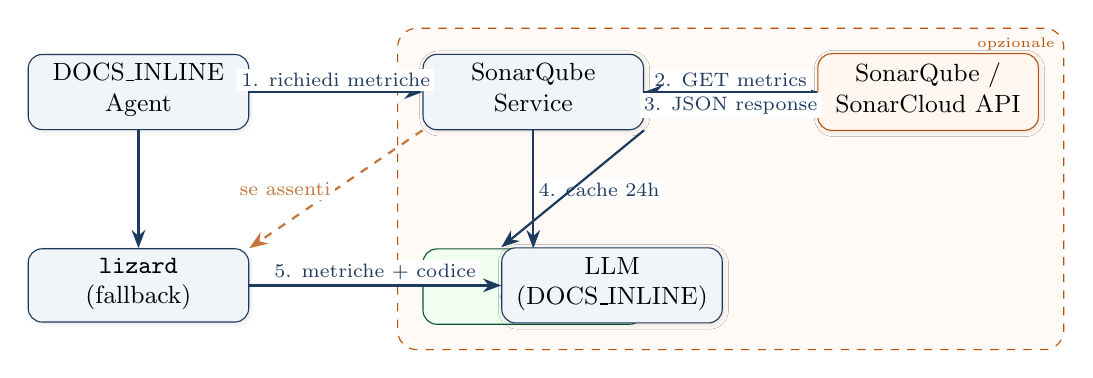
\begin{tikzpicture}[node distance=1.5cm and 2.2cm]
  \node[as@component] (agent)  {DOCS\_INLINE\\Agent};
  \node[as@component, right=of agent]  (sqsvc) {SonarQube\\Service};
  \node[as@external,  right=of sqsvc]  (sqapi) {SonarQube /\\SonarCloud API};
  \node[as@store,     below=1.5cm of sqsvc] (redis) {Redis\\Cache};
  \node[as@component, below=1.5cm of agent] (lizard) {\texttt{lizard}\\(fallback)};
  \node[as@component, right=3.2cm of lizard] (llm) {LLM\\(DOCS\_INLINE)};

  \draw[as@arr] (agent)  -- node[as@lbl,above]{1. richiedi metriche}  (sqsvc);
  \draw[as@arr] (sqsvc)  -- node[as@lbl,above]{2. GET metrics}        (sqapi);
  \draw[as@arr] (sqapi)  -- node[as@lbl,below]{3. JSON response}      (sqsvc);
  \draw[as@arr] (sqsvc.south) -- node[as@lbl,right]{4. cache 24h}    (redis.north);
  \draw[as@opt] (sqsvc.south west) -- node[as@lbl,left]{se assenti} (lizard.north east);
  \draw[as@arr] (agent.south)  -- (lizard.north);
  \draw[as@arr] (lizard.east)     -- node[as@lbl,above]{5. metriche + codice} (llm.west);
  \draw[as@arr] (sqsvc.south east) -- (llm.north west);

  \begin{scope}[on background layer]
    \node[draw=cg-amber, dashed, fill=orange!4, rounded corners=7pt,
          fit=(sqsvc)(sqapi)(redis), inner sep=9pt,
          label={[font=\tiny\color{cg-amber},anchor=north east]
                 north east:{opzionale}}] {};
  \end{scope}
\end{tikzpicture}
\caption{Flusso SonarQube nel DOCS\_INLINE agent. Il blocco tratteggiato è il percorso opzionale; in assenza di credenziali il flusso scende direttamente a \texttt{lizard}.}
\label{fig:be-sonarqube-flusso}
\end{figure}

\subsubsection{DOCS\_API (RF.86)}
Nuovo OperationCode, nuova voce in \texttt{AgentRegistry}, stessa sequenza Proposal→PR→URL. Cosa costituisca ``documentazione degli endpoint'' è una decisione del servizio agenti.

\subsection{Agente Security}
\label{sec:be-agente-security}

L'Agente Security è \emph{flag-only}: individua e documenta, non propone modifiche al repository. Il backend non apre mai Pull Request per queste operazioni.

\subsubsection{SECURITY\_OWASP (RF.87--RF.91)}
\label{sec:be-security-owasp}

Instradamento: \texttt{AgentRegistry} → Agente Security. Il backend invoca l'agente e persiste il Report ricevuto senza ulteriori passi. A partire dall'MVP, l'operazione articola l'esecuzione in due fasi sequenziali che affiancano l'analisi LLM con uno strumento SAST deterministico.

\paragraph{Integrazione SAST con Semgrep.}

Il SECURITY agent integra \textbf{Semgrep} (open source, \texttt{semgrep $\geq$ 1.80}) come primo stadio dell'analisi. Semgrep viene invocato come subprocess nell'ambiente container dell'agente: non richiede server esterni né credenziali aggiuntive. Le regole vengono scaricate una volta durante la build dell'immagine Docker e memorizzate localmente, rendendo ogni esecuzione offline e riproducibile.

\subsubsection*{DA-AS-3 \textemdash{} Esecuzione locale come subprocess, timeout 120\,s}
Semgrep è limitato a 120\,s (\texttt{-{}-timeout}). Il budget ADR-3 del SECURITY agent è 180\,s: i restanti 60\,s sono riservati alla chiamata LLM. Se Semgrep supera il limite, l'agente degrada a sola analisi LLM, segnalando il timeout nel report senza esporre errori all'utente. File superiori a 1\,MB sono esclusi dalla scansione statica e affidati interamente all'LLM (\texttt{-{}-max-target-bytes 1000000}).

\medskip
\noindent\textbf{Comando subprocess e mapping dell'output.} Il subprocess Semgrep viene invocato con:

\begin{lstlisting}[language=bash, caption={Comando Semgrep invocato dal SECURITY agent come subprocess.}]
semgrep \
  --config p/owasp-top-ten \
  [--config p/python]           # aggiunto se Python rilevato
  [--config p/typescript]       # aggiunto se TypeScript/JavaScript rilevato
  [--config p/nodejs-scan]      # aggiunto se TypeScript/JavaScript rilevato
  --json --quiet \
  --timeout $SEMGREP_TIMEOUT_S \
  --max-target-bytes 1000000 \
  /path/to/cloned/repo
\end{lstlisting}

\noindent Il mapping dai campi JSON dell'output Semgrep ai campi di \texttt{SASTFindingBlock} è:

\begin{center}
\renewcommand{\arraystretch}{1.15}
\begin{tabular}{ll}
\toprule
\texttt{SASTFindingBlock} & Campo JSON Semgrep \\
\midrule
\texttt{ruleId}           & \texttt{check\_id} \\
\texttt{owaspCategory}    & \texttt{extra.metadata.owasp[0]}; \texttt{'UNCLASSIFIED'} se assente \\
\texttt{severity}         & \texttt{extra.severity} (\texttt{ERROR}/\texttt{WARNING}/\texttt{INFO}) \\
\texttt{filePath}         & \texttt{path} (relativo alla root del repo) \\
\texttt{line}             & \texttt{start.line} \\
\texttt{message}          & \texttt{extra.message} (troncato a 500 caratteri) \\
\texttt{codeSnippet}      & \texttt{extra.lines} (troncato a 300 caratteri) \\
\texttt{cwe}              & \texttt{extra.metadata.cwe[0]}; omesso se assente \\
\bottomrule
\end{tabular}
\end{center}

\noindent \texttt{owaspCategory} è un campo stringa libera: le etichette OWASP nei metadati Semgrep non sono normalizzate e vengono passate direttamente all'LLM, che le usa per raggruppare i finding nel prompt.

\medskip
\noindent\textbf{Flusso in due fasi.}

\emph{Fase 1 --- Analisi statica.} Il rilevamento dei linguaggi avviene ispezionando le estensioni dei file nel repository clonato. In base ai linguaggi, viene selezionato il sottoinsieme di ruleset: il set \texttt{p/owasp-top-ten} è sempre incluso; per Python si aggiunge \texttt{p/python}, per TypeScript/JavaScript si aggiungono \texttt{p/typescript} e \texttt{p/nodejs-scan}. Semgrep produce un output JSON strutturato con i finding normalizzati nella struttura \texttt{SASTFinding} (definita in \S~\ref{ssec:be-sast-schema}).

\emph{Fase 2 --- Analisi LLM.} Prima dell'iniezione nel prompt, i finding vengono filtrati e ordinati in base a una soglia configurabile \texttt{SAST\_MAX\_FINDINGS\_LLM} (default \texttt{40}). L'ordinamento avviene per priorità decrescente: \texttt{ERROR} $>$ \texttt{WARNING} $>$ \texttt{INFO}; a parità di severity, si privilegia la varietà di categoria OWASP. I finding con la stessa coppia \texttt{(ruleId, filePath)} vengono deduplicati (mantenuta la prima occorrenza per numero di riga). I finding oltre il cap non transitano per l'LLM e ricevono automaticamente \texttt{llmVerdict: 'NEEDS\_REVIEW'}; il loro conteggio è riportato in \texttt{SASTSummary.cappedFindings}. I finding selezionati vengono iniettati nel prompt di sistema dell'agente, raggruppati per categoria OWASP. L'LLM determina per ogni finding se si tratta di un vero positivo nel contesto specifico, assegna un verdetto (\texttt{CONFIRMED}, \texttt{FALSE\_POSITIVE} o \texttt{NEEDS\_REVIEW}), propone remediation contestualizzate per i finding confermati e identifica vulnerabilità che l'analisi statica non rileva (logica applicativa, race condition, business logic flaw).

\medskip
\noindent Il Report persiste sia i \texttt{FindingBlock} classici prodotti dall'LLM sia i \texttt{SASTFindingBlock} arricchiti con il verdetto LLM (cfr.~\S~\ref{ssec:be-sast-schema}).

\begin{figure}[h!]
\centering
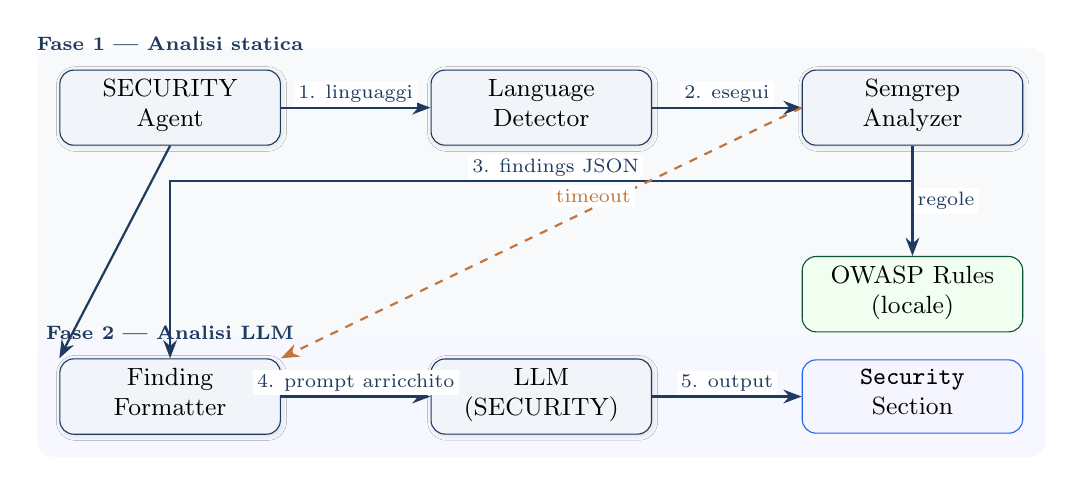
\begin{tikzpicture}[node distance=1.4cm and 1.9cm]
  \node[as@component] (agent)  {SECURITY\\Agent};
  \node[as@component, right=of agent]  (detect)  {Language\\Detector};
  \node[as@component, right=of detect] (semgrep) {Semgrep\\Analyzer};
  \node[as@store, below=1.4cm of semgrep] (rules) {OWASP Rules\\(locale)};
  \node[as@component, below=2.7cm of agent] (fmt)    {Finding\\Formatter};
  \node[as@component, right=of fmt]          (llm)    {LLM\\(SECURITY)};
  \node[as@output,    right=of llm]          (report) {\texttt{Security}\\Section};
  \node[font=\scriptsize\bfseries\color{cg-navy}, above=0.12cm of agent]   {Fase 1 --- Analisi statica};
  \node[font=\scriptsize\bfseries\color{cg-navy}, above=0.12cm of fmt]     {Fase 2 --- Analisi LLM};
  \draw[as@arr] (agent)   -- node[as@lbl,above]{1. linguaggi}   (detect);
  \draw[as@arr] (detect)  -- node[as@lbl,above]{2. esegui}      (semgrep);
  \draw[as@arr] (semgrep) -- node[as@lbl,right]{regole}         (rules);
  \draw[as@arr] (semgrep.south) -- ++(0,-0.45) -| node[as@lbl,above right, pos=0.3]{3. findings JSON} (fmt.north);
  \draw[as@arr] (agent.south)   -- (fmt.north west);
  \draw[as@arr] (fmt)    -- node[as@lbl,above]{4. prompt arricchito} (llm);
  \draw[as@arr] (llm)    -- node[as@lbl,above]{5. output}            (report);
  \draw[as@opt] (semgrep.west) -- node[as@lbl, above, pos=0.4]{timeout} (fmt.north east);
  \begin{scope}[on background layer]
    \node[fill=cg-light!60, rounded corners=6pt, fit=(agent)(detect)(semgrep)(rules), inner sep=8pt] {};
    \node[fill=blue!3, rounded corners=6pt, fit=(fmt)(llm)(report), inner sep=8pt] {};
  \end{scope}
\end{tikzpicture}
\caption{Flusso SAST nel SECURITY agent. La freccia tratteggiata indica il percorso di graceful degradation in caso di timeout Semgrep: i finding vengono omessi e il prompt LLM segnala l'assenza dell'analisi statica.}
\label{fig:be-sast-flusso}
\end{figure}

\subsubsection{SECURITY\_POLICY (RF.92, RF.93)}
Stessa meccanica di SECURITY\_OWASP, instradato su \texttt{SECURITY\_POLICY}. L'assenza di \texttt{POLICY.md} emerge come \texttt{CONTEXT\_RESOURCE\_MISSING} (RF.70) dall'agente, propagata dal backend come qualsiasi altro fallimento.

\subsection{Agente Changelog}
\label{sec:be-agente-changelog}

L'Agente Changelog non apre mai Pull Request: il suo output è testo. È l'unico agente che richiede input interattivi durante l'esecuzione.

\subsubsection{Flusso di input per le operazioni Changelog}

Entrambe le operazioni Changelog richiedono lo Sprint ID \emph{prima} dell'invocazione dell'agente. Il backend intercetta questo passo:
\begin{enumerate}
    \item \textbf{Sospensione pre-avvio} (\texttt{SPRINT\_ID}): se lo Sprint ID non è noto, NestJS valorizza \texttt{pendingInput = \{kind: "SPRINT\_ID"\}} ed emette \texttt{task.inputRequired} \emph{senza} invocare l'agente. L'utente risponde via \texttt{POST /tasks/:id/input}; solo allora l'agente viene avviato con lo Sprint ID nel payload.
    \item \textbf{Sospensione durante esecuzione} (\texttt{INCOMPLETE\_TASKS}): il \texttt{ChangelogLoader} (agente) rileva Issue con metadati insufficienti. Invece di procedere autonomamente, si sospende con \texttt{interrupt()} e restituisce al backend \texttt{\{kind: "INCOMPLETE\_TASKS", taskIds: [...]\}}. Il backend valorizza \texttt{pendingInput} e notifica il frontend. L'utente sceglie PROCEED (escludi gli elementi) o CANCEL (termina la Task in CANCELLED).
    \item \textbf{Sospensione durante esecuzione} (\texttt{BUSINESS\_CONFIRMATION}, solo CHANGELOG\_BUSINESS): il backend, dopo aver persistito il changelog tecnico come Report COMPLETED, valorizza \texttt{pendingInput = \{kind: "BUSINESS\_CONFIRMATION", technicalReportId: "<id>"\}} e sospende. L'utente legge il report tecnico (tramite \texttt{GET /reports/:id}), poi sceglie PROCEED (avvia fase business) o CANCEL (Task in CANCELLED).
\end{enumerate}

\subsubsection{CHANGELOG\_TECHNICAL (RF.94--RF.96)}
Il backend riceve lo Sprint ID da \texttt{POST /tasks/:id/input}, avvia l'agente con quel dato, persiste il Report tecnico ricevuto (un \texttt{TextBlock} in Markdown) e porta la Task a COMPLETED.

\subsubsection{CHANGELOG\_BUSINESS (RF.94--RF.105)}
Stessa sequenza di CHANGELOG\_TECHNICAL per la prima fase (changelog tecnico). Dopo la persistenza del Report tecnico, il backend sospende su \texttt{BUSINESS\_CONFIRMATION}. Alla conferma, riprende l'agente per la fase business; al rifiuto, porta la Task a CANCELLED. Una Task CHANGELOG\_BUSINESS che rifiuti la conferma non produce mai un changelog di business: chi vuole solo il changelog tecnico avvia CHANGELOG\_TECHNICAL.

\subsubsection{Leggibilità del Changelog (RQ.7)}
L'agente calcola l'indice Flesch Reading Ease sul proprio output. Se l'output non supera la soglia entro il budget di tentativi, l'agente restituisce \texttt{READABILITY\_TOO\_LOW}: il backend propaga il fallimento come ogni altro errore rilevato dall'agente.

%% ============================================================
\section{Gestione degli Errori}
\label{sec:be-errori}

\subsection{Il meccanismo riusato dalla PoC (RF.65)}

Il contratto della PoC copre già il percorso di errore di base: timeout e parsing failure valorizzano \texttt{error} e portano \texttt{status} a \texttt{FAILED} senza crash (PoC §5). Restano invariati: il campo \texttt{error: \{code, message, stage\} | null} su \texttt{TaskDto} e \texttt{ReportDto}; lo stato terminale \texttt{FAILED}; l'evento \texttt{task.failed}; l'isolamento dei fallimenti nel \texttt{TaskProcessor}.

\textbf{Correzione al contratto PoC}: \texttt{reportId} su \texttt{TaskDto} è valorizzato quando \texttt{status} è \texttt{COMPLETED} \emph{oppure} \texttt{FAILED} (non solo COMPLETED come indicato in PoC §7.4). Una Task fallita produce sempre un Report con \texttt{status: FAILED} e corpo vuoto, raggiungibile a \texttt{GET /reports/:id}: è ciò che permette al frontend di aprire il report da una Task fallita.

\subsection{Codici d'errore (enumerazione chiusa)}
\label{sec:be-codici-errore}

\begin{table}[H]
\centering
\caption{Enumerazione \texttt{error.code}: 11 valori per l'MVP. I messaggi mostrati all'utente restano quelli della Progettazione Frontend, Tabella~7.}
\label{tab:be-error-codes}
\vspace{2mm}
\renewcommand{\arraystretch}{1.2}
\begin{tabularx}{\textwidth}{|l|l|l|X|}
\hline
\textbf{\texttt{error.code}} & \textbf{Req.} & \textbf{Rilevato da} & \textbf{Azione secondaria (Frontend)} \\ \hline
\texttt{USAGE\_LIMIT\_EXCEEDED} & RF.66 & backend & Nessuna \\ \hline
\texttt{LLM\_TIMEOUT} & RF.67 & agente & ``Riprova'' \\ \hline
\texttt{LLM\_RATE\_LIMITED} & RQ.8 & agente & Da definire \\ \hline
\texttt{OUTPUT\_UNPARSABLE} & RF.68 & agente & ``Riprova'' \\ \hline
\texttt{CONTEXT\_TOO\_LARGE} & RF.69 & agente & Rimanda a \texttt{/select} \\ \hline
\texttt{CONTEXT\_RESOURCE\_MISSING} & RF.70 & agente & Nessuna \\ \hline
\texttt{CONTEXT\_RESOURCE\_INVALID} & RF.71 & agente & Nessuna \\ \hline
\texttt{READABILITY\_TOO\_LOW} & RQ.7 & agente & Da definire \\ \hline
\texttt{PR\_CREATION\_FAILED} & RF.72 & backend & Rimanda a \texttt{/credentials} \\ \hline
\texttt{CREDENTIAL\_INVALID} & RF.13, RS.4 & backend & Rimanda a \texttt{/credentials} \\ \hline
\texttt{INTERNAL\_ERROR} & RF.65 & backend & ``Riprova'' (fallback) \\ \hline
\end{tabularx}
\end{table}

\textbf{Regole di classificazione}: \texttt{INTERNAL\_ERROR} è il valore di ripiego per qualsiasi fallimento non previsto. Un'irraggiungibilità di rete verso GitHub ricade sempre in \texttt{INTERNAL\_ERROR} e mai in \texttt{CREDENTIAL\_INVALID} (per evitare falsi avvisi di credenziale non valida in caso di caduta del NAT Gateway). \texttt{error.stage} è sempre valorizzato con la fase in cui l'esecuzione si è interrotta per i codici rilevati durante l'esecuzione di una Task; i codici che nascono prima che una Task esista (\texttt{USAGE\_LIMIT\_EXCEEDED}, \texttt{CREDENTIAL\_INVALID} su POST /credentials) viaggiano nell'involucro di errore REST, non nel campo \texttt{error} di una Task.

\paragraph{Responsabilità di rilevamento}: gli agenti rilevano RF.67--RF.71, RQ.7--RQ.8 e restituiscono il codice al backend; il backend riceve, classifica e propaga (porta la Task a FAILED, valorizza \texttt{error}, persiste il Report fallito, emette \texttt{task.failed}). Il backend rileva in proprio solo RF.66 (limite utilizzo) e RF.72 (apertura PR).

\paragraph{Fallimento dell'apertura PR (RF.72)}: \texttt{PR\_CREATION\_FAILED} per rifiuto di autorizzazione GitHub (\texttt{error.stage = 'PULL\_REQUEST'}); \texttt{INTERNAL\_ERROR} per irraggiungibilità di rete. Il Report è persistito con il diff dell'agente prima del tentativo di apertura; quando il tentativo fallisce, il Report è aggiornato a status FAILED con l'errore. Il diff è conservato nei dati ma non offerto nell'interfaccia.

\subsection{Enumerazione \texttt{ErrorKind} lato agente (Python)}

Il backend riceve il codice di errore nell'oggetto \texttt{AgentStepResult.error}. Internamente, il servizio Python mappa ogni classe di fallimento su un \texttt{ErrorKind} prima di rispondere. L'MVP estende l'enumerazione del PoC (che copriva solo \texttt{TIMEOUT} e \texttt{PARSING}) con i codici aggiuntivi richiesti dai nuovi requisiti:

\begin{lstlisting}[language=Python, caption={\texttt{ErrorKind}: enumerazione estesa per l'MVP nel servizio agenti Python. I tre valori storici del PoC sono invariati; i cinque nuovi valori coprono i requisiti RF.69--RF.71, RQ.7--RQ.8.}]
from enum import Enum

class ErrorKind(str, Enum):
    # Valori storici (PoC)
    TIMEOUT  = "TIMEOUT"   # Timeout LLM (RF.67) -> error.code LLM_TIMEOUT
    PARSING  = "PARSING"   # Output LLM non parsabile (RF.68) -> OUTPUT_UNPARSABLE
    UPSTREAM = "UPSTREAM"  # Errore generico upstream -> INTERNAL_ERROR

    # Valori nuovi (MVP)
    CONTEXT_TOO_LARGE        = "CONTEXT_TOO_LARGE"        # RF.69
    CONTEXT_RESOURCE_MISSING = "CONTEXT_RESOURCE_MISSING" # RF.70
    CONTEXT_RESOURCE_INVALID = "CONTEXT_RESOURCE_INVALID" # RF.71
    READABILITY_TOO_LOW      = "READABILITY_TOO_LOW"      # RQ.7
    RATE_LIMITED             = "RATE_LIMITED"             # RQ.8 -> LLM_RATE_LIMITED
\end{lstlisting}

La mappatura da \texttt{ErrorKind} a \texttt{error.code} (backend) è biunivoca: \texttt{TIMEOUT} $\rightarrow$ \texttt{LLM\_TIMEOUT}, \texttt{PARSING} $\rightarrow$ \texttt{OUTPUT\_UNPARSABLE}, \texttt{RATE\_LIMITED} $\rightarrow$ \texttt{LLM\_RATE\_LIMITED}, gli altri tre nuovi valori mantengono il nome invariato come \texttt{error.code}.

%% ============================================================
\section{Report: Storico, Dettaglio ed Esportazione}
\label{sec:be-report}

\subsection{Contratto \texttt{ReportDto} esteso (RF.54--RF.64)}

Il Report estende l'envelope PoC con nuovi campi. Nessun campo esistente viene rimosso o rinominato:

\begin{lstlisting}[caption={\texttt{ReportDto}: schema completo di \texttt{GET /reports/:id} per l'MVP.}]
interface ReportDto {
  id: string
  taskId: string
  operation: OperationCode
  status: 'COMPLETED' | 'FAILED'
  title: string            // RF.51, sempre presente, deterministico
  summary: string | null   // null su report FAILED (nessun output agente)
  generatedAt: string      // ISO 8601 con offset (RF.52, RF.58)
  executionTimeMs: number | null   // RF.57; null se nessun agente invocato
  context: {               // RF.55-56, denormalizzato al momento del Report
    repoOwner: string
    repoName: string
    repoUrl: string
    branch: string
    resolvedSha: string
    scopeType: 'FULL_REPOSITORY' | 'FILES' | 'DIRECTORIES'
    paths: string[]
  }
  body: Block[]
  proposal?: {
    targetPath: string
    diffUnified: string
    language: string
    pullRequestUrl: string | null   // RF.63; null per Security e Changelog
  }
  pendingAction: {                  // RF.64, proiezione read-only di pendingInput
    kind: 'BUSINESS_CONFIRMATION'
    taskId: string
    actions: ('PROCEED' | 'CANCEL')[]
  } | null
  error?: { code: string; message: string; stage: string }
}
\end{lstlisting}

\textbf{Note implementative}:
\begin{itemize}
    \item \textbf{Titolo} (RF.51): composto deterministicamente dal backend nella forma \emph{``Nome operazione --- owner/repo@branch''} (es.\ ``Scansione OWASP --- SkynetUniGroup/Code\_Guardian@main''). Non generato da LLM; sempre presente anche su Report FAILED; letto dallo stesso catalogo di \texttt{GET /operations}.
    \item \textbf{Contesto denormalizzato}: i valori di \texttt{context} sono copiati nel documento Report al momento dell'assemblaggio, non risolti dinamicamente. Un report è un registro immutabile: resta leggibile anche se il contesto di analisi viene rimosso.
    \item \textbf{executionTimeMs} (RF.57): misura il solo \emph{tempo macchina}, cioè la somma dei segmenti di esecuzione dell'agente. Esclude: attesa in coda prima dell'invocazione, generazione PDF, e soprattutto i periodi di attesa dell'utente su \texttt{pendingInput} (che possono essere arbitrariamente lunghi). Il campo \texttt{Task.accumulatedMs} (campo interno, non esposto nell'API) accumula la durata di ciascuna chiamata \texttt{/internal/agent/*}; al completamento della Task, \texttt{Report.executionTimeMs} è scritto uguale a \texttt{Task.accumulatedMs}. Per le operazioni con una sola chiamata all'agente, \texttt{executionTimeMs = t\_response - t\_call}; per CHANGELOG\_BUSINESS, è la somma dei tre segmenti:
    \[
      \texttt{executionTimeMs} = (t_1 - t_0) + (t_2 - \text{risposta INCOMPLETE\_TASKS}) + (t_3 - t_2)
    \]
    dove $t_0, t_1, t_2, t_3$ sono i timestamp di chiamata e risposta di ciascuna invocazione \texttt{/internal/agent/*}.
    \item \textbf{pendingAction}: proiezione in sola lettura di \texttt{Task.pendingInput}. La risposta dell'utente viaggia sempre su \texttt{POST /tasks/:id/input}, mai tramite il Report.
    \item \textbf{Su Report FAILED}: \texttt{executionTimeMs} e \texttt{summary} valgono \texttt{null} se nessun agente è stato invocato. \texttt{body} è vuoto. \texttt{title} è sempre presente.
\end{itemize}

\subsection{Storico e sintesi (\texttt{GET /reports})}
\label{sec:be-report-storico}

\begin{lstlisting}[caption={\texttt{ReportSummaryDto}: proiezione restituita da \texttt{GET /reports}.}]
interface ReportSummaryDto {
  id: string             // RF.50
  operation: OperationCode
  status: 'COMPLETED' | 'FAILED'
  title: string          // RF.51
  generatedAt: string    // RF.52
}
\end{lstlisting}

\texttt{body}, \texttt{proposal} ed \texttt{error} sono esclusi dalla proiezione. L'endpoint è protetto da JWT; il guard confronta \texttt{Report.userId} con il claim \texttt{sub}: risposta 404 (non 403) se il report non appartiene al chiamante, per non confermare l'esistenza di report altrui.

\subsection{Blocchi del corpo (RF.59--RF.62)}

Due nuovi tipi di blocco, aggiuntivi rispetto ai \texttt{TextBlock} della PoC:

\begin{lstlisting}[caption={Nuovi tipi di blocco per l'MVP.}]
// Avviso di complessita' eccessiva (DOCS_INLINE, DOCS_API; mai DOCS_README)
interface ComplexityWarningBlock {
  kind: 'COMPLEXITY_WARNING'
  category: 'EXCESSIVE_COMPLEXITY'
  severity: 'LOW' | 'MEDIUM' | 'HIGH' | 'CRITICAL'  // valore fisso, non LLM
  filePath: string
  lineStart: number
  lineEnd: number
  reason: string
}

// Tipo di rimedio (union discriminata su kind)
// Usato in FindingBlock e PolicyViolationBlock
type Remediation =
  | { kind: 'SNIPPET'; language: string; code: string }
  | { kind: 'TEXT'; text: string }

// Riscontro di sicurezza OWASP (SECURITY_OWASP)
interface FindingBlock {
  kind: 'FINDING'
  category: string        // categoria OWASP
  severity: 'LOW' | 'MEDIUM' | 'HIGH' | 'CRITICAL'
  filePath: string
  lineStart: number
  lineEnd?: number
  description: string
  remediation: Remediation
}

// Violazione di policy (solo SECURITY_POLICY, RF.92--RF.93)
// Differisce da FindingBlock: porta rule_id/rule_text anziche' category OWASP.
// severity e' determinato dal modello (non valore fisso come in ComplexityWarningBlock).
interface PolicyViolationBlock {
  kind: 'POLICY_VIOLATION'
  ruleId: string                                     // identificatore della regola violata
  ruleText: string                                   // testo della regola (estratto da POLICY.md)
  filePath: string
  lineStart?: number
  lineEnd?: number
  severity: 'LOW' | 'MEDIUM' | 'HIGH' | 'CRITICAL'  // RF.61; determinato dal modello
  explanation: string
  remediation: Remediation
}
\end{lstlisting}

Il Markdown nei \texttt{TextBlock} è normalizzato dal backend al momento dell'assemblaggio: blocchi HTML grezzi rimossi, destinazioni \texttt{javascript:} e \texttt{data:} rifiutate. La normalizzazione avviene una volta sola, al confine, così resa a schermo ed esportazione PDF consumano la stessa stringa.

\subsection{Struttura \texttt{SASTFinding} e estensione \texttt{SecuritySection}}
\label{ssec:be-sast-schema}

L'integrazione SAST per \texttt{SECURITY\_OWASP} (\S~\ref{sec:be-security-owasp}) aggiunge un nuovo tipo di blocco al corpo del Report e due nuovi campi di primo livello alla sezione di sicurezza.

\noindent\textbf{Blocco \texttt{SASTFindingBlock}.} Ogni finding Semgrep arricchito con il verdetto LLM produce un blocco del tipo:

\begin{lstlisting}[caption={Tipo \texttt{SASTFindingBlock}: finding SAST con verdetto LLM (SECURITY\_OWASP).}]
interface SASTFindingBlock {
  kind: 'SAST_FINDING'
  ruleId: string           // identificatore della regola Semgrep
  owaspCategory: string    // es. 'A03:2021 - Injection'
  severity: 'ERROR' | 'WARNING' | 'INFO'  // severity Semgrep
  filePath: string
  line: number
  message: string
  codeSnippet: string      // estratto di codice (max 300 caratteri)
  cwe?: string             // CWE associato, se presente nei metadati regola
  llmVerdict: 'CONFIRMED' | 'FALSE_POSITIVE' | 'NEEDS_REVIEW'
  llmRemediation?: string  // proposta LLM; presente solo se CONFIRMED
}
\end{lstlisting}

\noindent\textbf{Campo \texttt{sastSummary}.} Il \texttt{ReportDto} di un'operazione \texttt{SECURITY\_OWASP} è esteso con un campo opzionale \texttt{sastSummary} che riporta l'esito aggregato della scansione:

\begin{lstlisting}[caption={Campo \texttt{sastSummary} nel \texttt{ReportDto} per SECURITY\_OWASP.}]
// Presente solo quando Semgrep ha eseguito (ENABLE_SAST_SEMGREP=true)
interface SASTSummary {
  totalFindings: number      // finding totali Semgrep
  confirmedFindings: number  // confermati dall'LLM
  falsePositives: number     // rigettati come falsi positivi
  needsReview: number        // non determinati (inclusi i finding oltre il cap)
  cappedFindings: number     // finding oltre SAST_MAX_FINDINGS_LLM, non
                             //   valutati dall'LLM (llmVerdict: NEEDS_REVIEW)
  scannedFiles: number       // file analizzati da Semgrep
  durationMs: number         // durata scansione
  timedOut: boolean          // true se Semgrep ha raggiunto il timeout
}
\end{lstlisting}

\subsection{Esportazione PDF (RF.73--RF.74)}
\label{sec:be-report-export}

\textbf{Endpoint}: \texttt{GET /reports/:id/export?format=pdf} (stesso percorso della PoC, formato \texttt{md} decade). Protetto da JWT con la stessa regola di proprietà di \texttt{GET /reports/:id} (404 se non appartiene al chiamante). Restituisce 409 su report FAILED (corpo vuoto per costruzione).

\textbf{Implementazione}: il PDF è composto programmaticamente (\texttt{pdfkit}/\texttt{pdf-lib}) a partire dal \texttt{ReportDto} persistito --- mai dal DOM renderizzato. Viene archiviato nel bucket S3 privato (lifecycle 30 giorni) e restituito in streaming con \texttt{Content-Type: application/pdf}, \texttt{Content-Disposition: attachment}, nome file \texttt{code-guardian-<operation>-<reportId>.pdf}. La composizione avviene interamente in memoria prima di scrivere nel corpo della risposta (per evitare file troncati in caso di errore). Le URL pre-firmate S3 sono vietate dalla Progettazione Frontend §13.5: lo streaming è sempre same-origin.

\textbf{Fallimento dell'esportazione} (RF.74): 500 con \texttt{\{code: 'EXPORT\_FAILED', message\}}. Nessun evento WebSocket; né \texttt{Task.status} né \texttt{Report.status} vengono modificati. \texttt{EXPORT\_FAILED} non compare nell'enumerazione di §~\ref{sec:be-codici-errore} perché non è un fallimento di esecuzione Task (UC27).

\textbf{Nota di rischio}: la Progettazione AWS (Tabella~20) annota che il task backend da 0,5~vCPU e 1~GB è dimensionato per un servizio REST leggero e la generazione PDF non è stata validata con un test di carico su esportazioni concorrenti. Tale test è da eseguire prima del rilascio.

%% ============================================================
\section{Servizi di Analisi Statica: Configurazione e Dipendenze}
\label{sec:be-analisi-statica}
%% ============================================================

Questa sezione raccoglie le informazioni trasversali ai due servizi di analisi statica introdotti nell'MVP: l'integrazione SonarQube per \texttt{DOCS\_INLINE} (\S~\ref{sec:be-docs-inline}) e l'integrazione SAST/Semgrep per \texttt{SECURITY\_OWASP} (\S~\ref{sec:be-security-owasp}).

\subsection{Feature flags}
\label{ssec:be-as-flags}

Entrambe le integrazioni sono controllate da variabili d'ambiente nel \texttt{docker-compose.yml} e nella task definition AWS ECS, senza richiedere modifiche all'interfaccia utente:

\begin{center}
\begin{tabular}{lll}
\toprule
Variabile & Default & Comportamento \\
\midrule
\texttt{ENABLE\_SONARQUBE} & \texttt{false} & Abilita il fetch metriche SonarQube per \texttt{DOCS\_INLINE} \\
\texttt{ENABLE\_SAST\_SEMGREP} & \texttt{true} & Abilita la scansione Semgrep per \texttt{SECURITY\_OWASP} \\
\texttt{SEMGREP\_TIMEOUT\_S} & \texttt{120} & Timeout subprocess Semgrep \\
\texttt{SONAR\_CACHE\_TTL\_S} & \texttt{86400} & TTL cache Redis per metriche SonarQube (24\,h) \\
\texttt{SAST\_MAX\_FINDINGS\_LLM} & \texttt{40} & Cap finding Semgrep iniettati nel prompt LLM; quelli oltre il limite ricevono \texttt{NEEDS\_REVIEW} automaticamente \\
\bottomrule
\end{tabular}
\end{center}

\subsection{Dipendenze aggiuntive}
\label{ssec:be-as-deps}

Le due integrazioni richiedono le seguenti aggiunte al file \texttt{requirements.txt} del servizio agenti Python:

\begin{itemize}
  \item \textbf{\texttt{semgrep $\geq$ 1.80}}: SAST engine e CLI. Include il proprio parser Python e non richiede binari aggiuntivi nel container. Le regole vengono scaricate durante la build dell'immagine Docker e memorizzate localmente.
  \item \textbf{\texttt{httpx $\geq$ 0.27}}: già presente come dipendenza esistente; usato per le chiamate HTTP alle API SonarQube.
  \item \textbf{\texttt{lizard}}: già presente; rimane il meccanismo base per la CC in \texttt{DOCS\_INLINE}.
\end{itemize}

\subsection{Budget temporale di \texttt{SECURITY\_OWASP} con SAST}
\label{ssec:be-as-budget}

\begin{center}
\begin{tabular}{clcc}
\toprule
\# & Azione & Durata tipica & Limite \\
\midrule
1 & Clone repository (già effettuato) & 5--20\,s & --- \\
2 & Rilevamento linguaggi & $<1$\,s & --- \\
3 & Scansione Semgrep & 15--100\,s & 120\,s (hard) \\
4 & Formattazione finding & $<1$\,s & --- \\
5 & Chiamata LLM con finding iniettati & 20--50\,s & --- \\
6 & Parsing e build \texttt{SecuritySection} & $<1$\,s & --- \\
\midrule
 & \textbf{Totale} & \textbf{41--172\,s} & \textbf{180\,s (ADR-3)} \\
\bottomrule
\end{tabular}
\end{center}

\end{document}

